\documentclass[11pt,a4paper]{article}
\usepackage[margin=2.4cm]{geometry}
\usepackage{amsmath,amsthm,mathtools}
\usepackage{fontspec}
\usepackage{unicode-math}
\setmainfont{texgyrepagella}[Path=fonts/, Extension=.otf,
  UprightFont=*-regular, ItalicFont=*-italic,
  BoldFont=*-bold, BoldItalicFont=*-bolditalic]
\setmathfont{texgyrepagella-math}[Path=fonts/, Extension=.otf]
% Pagella uses U+2216 for set difference.
\AtBeginDocument{\let\setminus\smallsetminus}
\usepackage[protrusion=true,expansion=false]{microtype}
\usepackage{booktabs,enumitem}
\usepackage{placeins}
\usepackage{tikz}
\usetikzlibrary{arrows.meta,positioning,calc,fit,backgrounds}
\definecolor{tierspend}{RGB}{200,60,60}
\definecolor{tierfull}{RGB}{210,140,40}
\definecolor{tierin}{RGB}{60,130,180}
\definecolor{tierrecv}{RGB}{70,150,90}
\usepackage[psdextra,hidelinks]{hyperref}

\emergencystretch=3em
\hbadness=10000
\hfuzz=2pt

\newtheorem{theorem}{Theorem}[section]
\newtheorem{lemma}[theorem]{Lemma}
\newtheorem{proposition}[theorem]{Proposition}
\newtheorem{corollary}[theorem]{Corollary}
\theoremstyle{definition}
\newtheorem{definition}[theorem]{Definition}
\newtheorem{construction}[theorem]{Construction}
\newtheorem{assumption}[theorem]{Assumption}
\newtheorem{remark}[theorem]{Remark}
\newtheorem{example}[theorem]{Example}

% kind-coded theorem blocks, palette shared with the figures and the website:
% definitions/constructions blue (tierin), assumptions amber (tierfull),
% proved statements a neutral bar; remarks and examples run unframed
\usepackage{mdframed}
\providecolor{tierin}{RGB}{60,130,180}
\providecolor{tierfull}{RGB}{210,140,40}
\mdfdefinestyle{kindbar}{topline=false,bottomline=false,rightline=false,
  linewidth=1.5pt,innerleftmargin=9pt,innerrightmargin=4pt,
  innertopmargin=5pt,innerbottommargin=6pt,leftmargin=0pt,rightmargin=0pt,
  skipabove=10pt,skipbelow=10pt}
\surroundwithmdframed[style=kindbar,linecolor=tierin!70,backgroundcolor=tierin!4]{definition}
\surroundwithmdframed[style=kindbar,linecolor=tierin!70,backgroundcolor=tierin!4]{construction}
\surroundwithmdframed[style=kindbar,linecolor=tierfull!80,backgroundcolor=tierfull!5]{assumption}
\surroundwithmdframed[style=kindbar,linecolor=black!30]{theorem}
\surroundwithmdframed[style=kindbar,linecolor=black!30]{lemma}
\surroundwithmdframed[style=kindbar,linecolor=black!30]{proposition}
\surroundwithmdframed[style=kindbar,linecolor=black!30]{corollary}

\usepackage{fancyhdr}
\pagestyle{fancy}
\fancyhf{}
\fancyhead[L]{\footnotesize\scshape The Zcash Arboretum}
\fancyhead[R]{\footnotesize\itshape\nouppercase{\leftmark}}
\fancyfoot[C]{\footnotesize\thepage}
\renewcommand{\headrulewidth}{0.3pt}
\renewcommand{\sectionmark}[1]{\markboth{\thesection\ \ #1}{}}

\newcommand{\F}{\mathbb{F}}
\newcommand{\Z}{\mathbb{Z}}
\newcommand{\N}{\mathbb{N}}
\newcommand{\G}{\mathbb{G}}
\newcommand{\E}{\mathbb{E}}
\newcommand{\PP}{\mathbb{P}}
\renewcommand{\Pr}{\mathrm{Pr}}
\newcommand{\Fp}{\F_p}
\newcommand{\Fq}{\F_q}
\newcommand{\ip}[2]{\langle #1,\, #2 \rangle}
\newcommand{\Comm}{\mathsf{Commit}}
\newcommand{\Open}{\mathsf{Open}}
\newcommand{\Setup}{\mathsf{Setup}}
\newcommand{\Verify}{\mathsf{Verify}}
\newcommand{\negl}{\mathsf{negl}}
\newcommand{\poly}{\mathsf{poly}}
\newcommand{\PPT}{\mathsf{PPT}}
\newcommand{\Adv}{\mathcal{A}}
\newcommand{\Prov}{\mathcal{P}}
\newcommand{\Ver}{\mathcal{V}}
\newcommand{\Sim}{\mathcal{S}}
\newcommand{\Ext}{\mathcal{E}}
\newcommand{\Rel}{\mathcal{R}}
\newcommand{\Lang}{\mathcal{L}}
\newcommand{\nfsym}{\mathsf{nf}}
\newcommand{\cmsym}{\mathsf{cm}}
\newcommand{\cmx}{\mathsf{cmx}}
\newcommand{\cvsym}{\mathsf{cv}}
\newcommand{\rk}{\mathsf{rk}}
\newcommand{\Pallas}{\ensuremath{\mathsf{Pallas}}}
\newcommand{\Vesta}{\ensuremath{\mathsf{Vesta}}}
\newcommand{\Ep}{\ensuremath{\mathcal{E}}}
\newcommand{\NoteCommit}{\ensuremath{\mathsf{NoteCommit}}}
\newcommand{\Sinsemilla}{\ensuremath{\mathsf{Sinsemilla}}}
\newcommand{\ShortCommit}{\ensuremath{\mathsf{ShortCommit}}}
\newcommand{\CommitIvk}{\ensuremath{\mathsf{Commit}^{\mathsf{ivk}}}}
\newcommand{\Extract}{\ensuremath{\mathsf{Extract}}}
\newcommand{\Acc}{\ensuremath{\mathsf{Acc}}}
\newcommand{\GroupHash}{\ensuremath{\mathsf{GroupHash}}}
\newcommand{\ask}{\ensuremath{\mathsf{ask}}}
\newcommand{\aksym}{\ensuremath{\mathsf{ak}}}
\newcommand{\nksym}{\ensuremath{\mathsf{nk}}}
\newcommand{\ivk}{\ensuremath{\mathsf{ivk}}}
\newcommand{\fvk}{\ensuremath{\mathsf{fvk}}}
\newcommand{\ovk}{\ensuremath{\mathsf{ovk}}}
\newcommand{\dk}{\ensuremath{\mathsf{dk}}}
\newcommand{\pkd}{\ensuremath{\mathsf{pk_d}}}
\newcommand{\gd}{\ensuremath{\mathsf{g_d}}}
\newcommand{\rcv}{\ensuremath{\mathsf{rcv}}}
\newcommand{\rcm}{\ensuremath{\mathsf{rcm}}}
\newcommand{\rivk}{\ensuremath{\mathsf{r_{ivk}}}}
\newcommand{\rsk}{\ensuremath{\mathsf{rsk}}}

\renewenvironment{abstract}{%
  \small\begin{center}{\bfseries\abstractname}\end{center}\medskip\noindent\ignorespaces
}{\par\medskip}

\title{\textbf{\Huge Ironwood Guide}\\[6pt]\large The Zcash Orchard protocol and its Ironwood pool}
\author{m@rek.onl}
\date{}
\begin{document}
\maketitle
\thispagestyle{empty}

\begin{abstract}
This volume of \emph{The Zcash Arboretum} constructs the Orchard protocol for a
shielded payment in its Ironwood pool: how the payment is constructed, delivered
to its recipient and verified; why a valid payment cannot create value, consume
a note twice or consume a note without the authority of its owner; and what its
public data hide. Every public field of the payment is constructed, in
dependency order, as a fixed function of private notes, keys and randomness; the
relation that each Action of the payment proves is stated over those objects;
and each security property is a theorem under named assumptions. The sealed
Orchard pool enters only where a rule shared with the Ironwood pool, or a rule
that distinguishes the two pools, is needed to state the Ironwood-pool payment
correctly. The volume assumes the \emph{Math Guide} and the \emph{Crypto Guide}
and cites the \emph{Halo 2 Guide} for the proof system. It is non-normative: the
Zcash Protocol Specification and the Zcash Improvement Proposals are
authoritative.
\end{abstract}
\clearpage
\tableofcontents
\clearpage

\section{Introduction}\label{sec:intro}

This section fixes the subject of the volume, its status and its vocabulary
before any construction: the scope; in plain language, the structure of a
shielded payment and the division of its verification; the Orchard protocol
and its two value pools; and the requirements that a shielded payment must
meet.

\subsection{Scope and status}\label{sec:intro-scope}

This volume of \emph{The Zcash Arboretum} constructs the Orchard protocol for
a shielded payment in the Ironwood pool, both terms being defined in
\S\ref{sec:intro-pools}: how the payment is constructed, delivered and
verified; why a valid payment cannot create value, consume a note twice, or
consume a note without the authority of its owner; and what it hides. The
sealed Orchard pool enters only where a rule shared with the Ironwood pool,
or a rule that distinguishes the two pools, is needed to state the
Ironwood-pool payment correctly. The volume assumes the \emph{Math Guide} and
the \emph{Crypto Guide}, and cites the \emph{Halo 2 Guide} for the proof
system. It is non-normative: the Zcash Protocol Specification, cited as the
protocol specification with the title of a section, and the Zcash
Improvement Proposals are authoritative.

\begin{definition}[Block chain, transaction, consensus rules]
A \emph{block chain} is a sequence of blocks that starts at the \emph{genesis
block}, the header of each block referring to the preceding block; the
\emph{height} of a block is its number of predecessors, so that the genesis
block has height $0$ (ZIP 200, Terminology; protocol specification, \S``The
Block Chain''). Each block contains an ordered sequence of one or more
\emph{transactions}, the units in which the chain records transfers of value
(protocol specification, \S``Transactions and Treestates''). The
\emph{consensus rules} are the validation rules that determine which block
chains, and hence which blocks and transactions, are valid (ZIP 200,
Terminology, ``Consensus rule set'').
\end{definition}

\begin{definition}[ZIP]
A \emph{Zcash Improvement Proposal} (ZIP) is a design document that
describes a feature of Zcash, or a change to it, with a concise technical
specification and a rationale. Each ZIP carries a status. Two statuses are
named in this volume: \emph{Draft}, the status that every ZIP receives on
submission, and \emph{Reserved}, the status of a ZIP number that the ZIP
editors have reserved while no ZIP text has been published (ZIP 0, Abstract
and ``ZIP Status Field''). A deployed rule is cited to a section of the
protocol specification by its title, or to a ZIP and its section.
\end{definition}

\begin{definition}[Network upgrade]
A \emph{network upgrade} is an intentional change of the consensus rules
that takes effect at a block height fixed for it, its \emph{activation
height}: blocks below that height are validated under the preceding rules,
and blocks at or above it under the new rules. Network upgrades are named and
activate in a fixed order (ZIP 200, Terminology and ``Activation
mechanism''). This volume names two: NU6.3, whose deployment ZIP is ZIP 258,
and NU7, the upgrade that follows NU6.3, whose deployment ZIP is ZIP 259
(ZIP 258, Abstract; ZIP 259, Abstract and Rationale, ``Rationale for no new
transaction format'').
\end{definition}

The volume describes the protocol as specified for NU7, whose deployment ZIP
has status Draft (ZIP 259, preamble). It names a network upgrade only where
the name fixes which rule applies, gives no activation parameter, such as an
activation height or a date, and describes no upgrade by what it adds or
changes.

\begin{definition}[Epistemic classes]
Where the status of a claim about the deployed protocol needs stating, the
volume places it in one of exactly two classes. The claim is
\emph{specified} when normative text of the protocol specification or of a
ZIP fixes it. It is \emph{designed but unspecified} when the deployed
construction is designed to satisfy it but neither the protocol
specification, nor a ZIP, nor a published proof establishes it for the
deployed instance. An example of each class is given where its object is
introduced: knowledge soundness of the Action proof in
\S\ref{sec:intro-structure}, and the cross-address restriction in
\S\ref{sec:intro-pools}.
\end{definition}

\subsection{The structure of a shielded payment}\label{sec:intro-structure}

This subsection names, in plain language, the objects of a shielded payment
and the checks that verify it. Each term receives one defining clause here
and its construction in the section named.

\begin{definition}[Notes, note commitments, nullifiers]
A shielded payment transfers value held in \emph{notes}. A note records,
among other fields, an amount of value and the \emph{address} of its
recipient, a public value derived from the recipient's keys
(\S\ref{sec:keys-addr}); no note is published in the clear
(\S\ref{sec:notes-note}). For each note that a payment creates, the chain
records a commitment to the note in the sense of the \emph{Crypto Guide},
\S``Hiding and binding'', its \emph{note commitment}, in the extracted form
constructed in \S\ref{sec:notes-cm}. For each note that a payment
consumes, the chain records a tag, the note's \emph{nullifier}, which marks
the note as consumed (\S\ref{sec:nf-nullifier}).
\end{definition}

\begin{definition}[Value pool]
In this volume a \emph{value pool} is a separately accounted collection of
notes with its own record of note commitments, the \emph{note commitment
tree} (\S\ref{sec:tree-hash}); its own record of nullifiers, the
\emph{nullifier set} (\S\ref{sec:nf-sets}); and its own \emph{chain value
pool balance}, the total value that the chain accounts as held in the pool
(\S\ref{sec:tx-pools}).
\end{definition}

\begin{definition}[Action, dummy note]
A shielded payment is carried by \emph{Actions}. An Action consumes one note
of a pool and creates one note of the same pool. A side of an Action that
the payment does not use carries a \emph{dummy note}, a note of value zero
that pads the Action (\S\ref{sec:notes-action}; protocol specification,
\S``Action Transfers and their Descriptions'' and \S``Dummy Notes
(Orchard)'').
\end{definition}

\begin{definition}[Bundle, balancing value]
The Actions of one transaction in one pool, together with data common to
them, form the transaction's \emph{bundle} for that pool; a transaction
carries at most one bundle per pool (\S\ref{sec:notes-action}; ZIP 229,
Abstract and ``Transaction Format''). The \emph{balancing value} of a bundle
is the net value, public, that the bundle moves out of its pool into the rest
of the transaction; it is negative when value enters the pool
(\S\ref{sec:value-balance}).
\end{definition}

\begin{definition}[Note ciphertext]
A created note reaches its recipient through the chain: the Action that
creates it also carries a \emph{note ciphertext}, an encryption of the note
to the recipient's address, from which the recipient recovers the note
(\S\ref{sec:enc}).
\end{definition}

\begin{remark}[Division of verification]
A \emph{verifier}, a party that checks transactions against the consensus
rules, accepts a bundle, without learning its notes, on one proof per
bundle, two kinds of signature and two checks against the state of the
chain (protocol specification, \S``Action Transfers and their
Descriptions'' and \S``Action Descriptions'').
\begin{enumerate}[label=(\arabic*)]
\item One zero-knowledge proof per bundle, the \emph{Action proof}
  (\emph{Crypto Guide}, \S``SNARKs: succinct non-interactive arguments of
  knowledge''; \emph{Halo 2 Guide}, \S``The Halo 2 proof system''): an
  argument that the prover knows, for
  each Action, private data that together with the Action's public data
  satisfy one fixed relation, in the sense of the \emph{Crypto Guide},
  \S``Languages, relations, and witnesses'', namely the Action statement,
  defined in ``The Action statement'' (\S\ref{sec:action-statement}). The
  proof system has no notion of value or ownership; the relation supplies
  both.
\item Per Action, a \emph{spend-authorisation signature} (\emph{Crypto
  Guide}, \S``Syntax and security goal''), made with a signing key obtained
  from the \emph{spend authorising key}, the signing secret associated with
  the consumed note's address (\S\ref{sec:keys-sk}), by which the holder of
  that key authorises the consumption (\S\ref{sec:spendauth}).
\item Per bundle, one \emph{binding signature}, by which balance is checked:
  the total value of the notes that the bundle consumes, minus that of the
  notes it creates, equals its balancing value (\S\ref{sec:value-bsig}).
\item Two checks against the state of the chain. The proof refers to one
  earlier state of the pool's note commitment tree, through a digest of that
  state, the bundle's \emph{anchor} (\S\ref{sec:tree-anchors}), and the
  verifier checks that the anchor is one that the chain recorded for an
  earlier block. The verifier also checks that every nullifier that the
  bundle publishes is new to the pool (\S\ref{sec:nf-sets}).
\end{enumerate}
Both kinds of signature sign one digest of the transaction, constructed in
``Transaction digests and signatures'' (\S\ref{sec:tx-sighash}). The two
checks of~(4) lie outside the proof because they concern the history of the
whole chain, which a proof over the data of one Action cannot attest.
\end{remark}

Knowledge soundness of the Action proof as deployed (\emph{Crypto Guide},
\S``SNARKs: succinct non-interactive arguments of knowledge''), the property
under which an accepted proof establishes the knowledge claimed in~(1), is
designed but unspecified: the volume takes it as
Assumption~\ref{ass:ks} (\S\ref{sec:action-circuit}), not as a result.

\subsection{The Orchard protocol and its two pools}\label{sec:intro-pools}

\begin{definition}[Orchard protocol]
The \emph{Orchard protocol} is the cryptographic design shared by two value
pools: its primitive instances, among them the Pallas and Vesta curves and
the Sinsemilla hash (\S\ref{sec:prim}); its keys and addresses; its notes,
note commitments and nullifiers; its note encryption; and the one relation
that every Action proves, the Action statement, defined in ``The Action
statement'' (\S\ref{sec:action-statement}), with the circuit designed to
encode it (\S\ref{sec:action-circuit}). ZIP 229 fixes this vocabulary
(ZIP 229, Terminology), and the volume adopts it.
\end{definition}

\begin{definition}[Orchard pool, Ironwood pool]
The \emph{Orchard pool} and the \emph{Ironwood pool} are the two value pools
of the Orchard protocol. Each has its own note commitment tree, and hence
its own anchors, its own nullifier set and its own chain value pool balance
(ZIP 229, Terminology, and Rationale, ``Separate state'').
\end{definition}

The Ironwood pool admits net inflow, value moved into it by a negative balancing
value (\S\ref{sec:tx-pools}). The Orchard pool is \emph{sealed}, in two respects
(ZIP 258, ``Consensus rules from~NU6.3 activation''); each rule is stated where
its object is constructed. First, no transaction increases the value held in the
Orchard pool (\S\ref{sec:tx-pools}). Second, every Orchard-pool Action creates
its note at the address of the note it consumes (ZIP 229, Rationale,
``\texttt{enableCrossAddress} polarity''), a rule made exact in ``Bundle flags''
(\S\ref{sec:action-flags}) and with the Action statement, defined in ``The
Action statement'' (\S\ref{sec:action-statement}). ZIP 229, Abstract, states the
effect of the second rule: outputs to the Orchard pool go to an address for
which the creator of the transaction can authorise spends, which discourages
transfers between users within the Orchard pool. Consensus does not prevent such
transfers: any party able to authorise spends for an address can create an
Orchard-pool note to that address, since the consumed side of the Action can be
a dummy note at that address (ZIP 326, ``Rationale for key-generation
restrictions''; the witness of such an Action is exhibited in
\S\ref{sec:action-statement}).

The restriction of an Action's created note to the address of its consumed
note, in force for every Orchard-pool Action and for every Ironwood-pool
Action whose bundle does not enable cross-address transfers
(\S\ref{sec:action-flags}), is specified: the protocol specification,
\S``Action Descriptions'', fixes the meaning of the flag that controls it,
although ZIP 2006, which that section cites for it, has status Reserved
(ZIP 2006, preamble).

Notes of the two pools have the same form and the same note commitment. They
differ only in the note plaintext format, the encoding in which note encryption
carries a note: an Ironwood-pool note uses the format whose first byte, the
\emph{lead byte} that names the format, is $\mathtt{0x03}$, under which the
note's \emph{commitment trapdoor}, the randomness of its note commitment, is
derived by hashing a random seed, which the plaintext carries, together with
every field that the commitment binds (the format and
the lead-byte rule in \S\ref{sec:notes-seed}, the plaintext in
\S\ref{sec:enc-plaintext}; ZIP 258, ``ZIP 2005 activation''). Actions of both
pools prove the same relation, the Action statement, defined in ``The Action
statement'' (\S\ref{sec:action-statement}), with one circuit and one
\emph{verifying key}, the public parameter against which a proof is checked
(\S\ref{sec:action-circuit}; protocol specification, \S``Action Descriptions'';
ZIP 258, ``Consensus rules from~NU6.3 activation''). The pools are distinguished
by their note commitment trees, nullifier sets and chain value pool balances,
and by the component of the transaction that carries their bundles
(\S\ref{sec:tx-format}), not by separate circuits (ZIP 229, Abstract, and
Rationale, ``Reuse of the Orchard protocol with minimal changes'').

Orchard-pool notes are spendable, in version-$5$ and version-$6$
transactions (\S\ref{sec:tx-format}), subject to the rules that seal the
Orchard pool (ZIP 258, ``Consensus rules from~NU6.3 activation''; ZIP 259,
Abstract).

The name ``Orchard'' alone qualifies the shared cryptography of the Orchard
protocol; a statement that depends on the pool names the pool, the Orchard
pool or the Ironwood pool.

\subsection{Requirements on a shielded payment}\label{sec:intro-req}

\begin{definition}[Transparent and shielded payments, observer]
A \emph{transparent payment} is one whose consumed and created amounts and
addresses are public. The goal of a shielded payment is to achieve the
effects of a transparent payment, namely transfer of value, exclusion of
\emph{double-spending}, the consumption of one note twice, and conservation
of value, while hiding the contents of its notes, and the links between the
notes it consumes and the notes it creates, from an \emph{observer}: any
party that reads the chain but holds no key of the notes concerned.
Requirements R1 to R5 below make this precise. Each of R1 to R4 has a
\emph{soundness part}, a property of every valid payment, and a
\emph{hiding part}, a bound on what the observer learns; R5 has a soundness
part only.
\end{definition}

\begin{definition}[Requirements R1 to R5]
\leavevmode
\begin{enumerate}[label=R\arabic*., leftmargin=2.4em]
\item \emph{Hidden representation of value.} Soundness: the chain's record
  of a created note binds that note, so that its owner can later prove
  possession of it and no party can present the record as the record of a
  different note. Hiding: the record reveals neither the recipient's address
  nor the value, and does not distinguish a real note from a dummy note.
\item \emph{Membership without identification.} Soundness: every consumed
  note of non-zero value was previously committed in the same pool, at the
  state of the pool's record of commitments to which the payment refers.
  Hiding: the payment does not identify which committed note it consumes. A
  note of value zero, such as a dummy note, transfers no value, and R2 does
  not require it to have been committed.
\item \emph{No second consumption.} Soundness: no note of a pool is consumed
  twice. Hiding: this holds without a public list of consumed notes; the
  data published when a note is consumed do not identify which committed
  note it is.
\item \emph{Conservation.} Soundness: in every valid bundle the total value
  of the consumed notes equals the total value of the created notes plus the
  balancing value, so that no payment creates value. Hiding: no note's value
  is disclosed; of the amounts, only the balancing value is public.
\item \emph{Spend authority}, a soundness part only. Only the holder of a
  note's spending authority, the spend authorising key associated with its
  address (\S\ref{sec:keys-sk}), can consume the note; and no
  other party can alter what an authorised payment transfers, namely the
  notes it consumes and creates and the value it moves into or out of the
  pool, without invalidating it. Requirement R5 requires nothing of data that
  do not change what is transferred; which data the signatures fix is stated
  in ``Transaction digests and signatures'' (\S\ref{sec:tx-sighash}).
\end{enumerate}
\end{definition}

The requirement map, Table~\ref{tab:action-req}, given with the Action
statement (\S\ref{sec:action-statement}), pairs the soundness and hiding
parts of each requirement with the results that discharge them; ``Security''
(\S\ref{sec:security}) states those results as theorems with their
assumptions.

\section{Notation and primitive instances}\label{sec:prim}

This section fixes the encodings and the primitive instances on which the
later constructions rest, each with its Orchard parameters and domain
separators. The underlying constructions belong to the \emph{Math Guide} and
the \emph{Crypto Guide} and are cited, not re-derived; each named assumption
is stated at the first construction whose security needs it.

\subsection{Fields, groups, and encodings}\label{sec:prim-fields}

The Pallas group $\Ep(\F_{p_{\Pallas}})$ is the group of points of the curve
$y^2 = x^3 + 5$ over the prime field $\F_{p_{\Pallas}}$, with identity
$\mathcal{O}$. It has prime order $p_{\Vesta}$ and cofactor $1$, and
$\F_{p_{\Vesta}}$ is both its scalar field and the base field of the Vesta
curve (\emph{Math Guide}, \S``Base fields, scalar fields, and the Pasta
cycle'' and \S``Pallas and Vesta assembled'', Example ``The Pasta curves'';
\emph{Crypto Guide}, \S``Instantiation on elliptic curves; the Pasta curves'',
Definition ``The Pasta curves''). The group, its order and the cycle with
Vesta are cited, not re-derived; the moduli are those of the protocol
specification, \S``Pallas and Vesta''. Table~\ref{tab:prim-notation} maps
this notation, once, to the names used by the specification and by the lower
volumes. Those names appear in the table only; later text writes only the
column headed ``This volume''. Maps defined on the Pallas group carry the
specification's subscript $\PP$, as in $\Extract_{\PP}$.

\begin{table}[ht]
\centering\small
\begin{tabular}{@{}p{5.3cm}lll@{}}
\toprule
Object & This volume & Specification & Lower volumes \\
\midrule
Pallas base-field modulus
  & $p_{\Pallas}$ & $q_{\mathbb{P}}$ & $p$ \\
Pallas scalar-field modulus, Vesta base-field modulus, order of the Pallas
group
  & $p_{\Vesta}$ & $r_{\mathbb{P}}$ & $q$ \\
Pallas base field and scalar field
  & $\F_{p_{\Pallas}}$, $\F_{p_{\Vesta}}$
  & $\F_{q_{\mathbb{P}}}$, $\F_{r_{\mathbb{P}}}$ & $\F_p$, $\F_q$ \\
Pallas group
  & $\Ep(\F_{p_{\Pallas}})$ & $\mathbb{P}$ & $E_p(\F_p)$ \\
$k$-bit little-endian encoding of an integer
  & $\mathrm{LE}_k$ & $\mathsf{I2LE{}BSP}_k$ & --- \\
Encoding of a point $P$
  & $P^{\star}$ & $\mathsf{repr}_{\mathbb{P}}(P)$ & --- \\
Sinsemilla short commitment
  & $\ShortCommit$ & $\mathsf{Sinsemilla{}ShortCommit}$ & --- \\
Spend validating key, as a point and as its $x$-coordinate
  & $\aksym^{\PP}$, $\aksym$ & $\aksym^{\mathbb{P}}$, $\aksym$ & --- \\
\bottomrule
\end{tabular}
\caption{Notation for the fields, the Pallas group and the encodings, with
the names of the protocol specification and of the \emph{Math} and
\emph{Crypto Guides}. The spend validating key is constructed in
\S\ref{sec:keys-sk}; the point $\aksym^{\PP}$ and the field element
$\aksym = \Extract_{\PP}(\aksym^{\PP})$ are kept apart throughout.}
\label{tab:prim-notation}
\end{table}

Scalar multiplication is written $[k]P$, for $k \in \F_{p_{\Vesta}}$ or an
integer read modulo $p_{\Vesta}$. The symbol $\|$ denotes concatenation of
bit strings or of byte strings, and $\varepsilon$ the empty string.
Byte-string literals and tags are set in monospace, as in
$\texttt{z.cash:Orchard}$, and single bytes as $\mathtt{0x..}$. The symbol
$\bot$ is the failure value of a partial map; a map that may fail takes
values in $X \cup \{\bot\}$ for its codomain $X$.

% compute/fields.py:
% [sec:prim-fields] bit length of p_Pallas = 255, of p_Vesta = 255;
%   p_Pallas < p_Vesta
% [sec:prim-fields] p_Vesta - p_Pallas = 0x47afc1f319ba3400000000
%   (about 2^86.16)
Both moduli have bit length $255$, and $p_{\Pallas} < p_{\Vesta}$:
\[
  2^{254} < p_{\Pallas} < p_{\Vesta} < 2^{255}.
\]
Two consequences are used later. First, the integer representative of an
element of either field lies in $\{0, \dots, 2^{255} - 1\}$ and has a
$255$-bit encoding, which leaves the top bit of a $256$-bit string free.
Second, the integer representative of an element of $\F_{p_{\Pallas}}$ lies
in $\{0, \dots, p_{\Vesta} - 1\}$; reading it as a Pallas scalar is
therefore an injective, not a surjective, map
$\F_{p_{\Pallas}} \to \F_{p_{\Vesta}}$. This map is used wherever a
base-field element multiplies a point (\S\ref{sec:keys-addr},
\S\ref{sec:nf-nullifier}).

\begin{definition}[Integer and byte encodings]
For $k \ge 0$ and an integer $m \in \{0, \dots, 2^k - 1\}$, the
\emph{$k$-bit little-endian encoding} $\mathrm{LE}_k(m) \in \{0,1\}^k$ is the
bit sequence $b_0 b_1 \cdots b_{k-1}$ with $m = \sum_{i=0}^{k-1} b_i 2^i$.
The map $\mathrm{LE}_k \colon \{0, \dots, 2^k - 1\} \to \{0,1\}^k$ is a
bijection with inverse $\mathrm{LE}_k^{-1}$. A field element is encoded
through its integer representative in $\{0, \dots, p - 1\}$, for $p$ the
modulus. In the conversion names below, $\mathsf{I}$ stands for integer,
$\mathsf{LE}$ for little-endian, $\mathsf{BS}$ for bit string, and
$\mathsf{OS}$ for octet string (a sequence of eight-bit bytes). The digit
$2$ is read ``to'', and $\mathsf{P}$ stands for primitive, a basic conversion
operation. The subscript $k$ counts bits, not bytes. Three maps relate
integers, bit strings and byte strings:
\begin{itemize}
\item the map $\mathsf{I2LEOSP}_k$ sends $m \in \{0, \dots, 2^k - 1\}$ to its
  $\lceil k/8 \rceil$-byte little-endian encoding;
\item for $k$ a multiple of $8$, the map $\mathsf{LEOS2IP}_k$ sends a
  $k/8$-byte string $(s_0, \dots, s_{k/8-1})$ to the integer
  $\sum_{i} s_i\, 256^i \in \{0, \dots, 2^k - 1\}$;
\item the map $\mathsf{LEBS2OSP}_k \colon \{0,1\}^k \to
  \{0, \dots, 255\}^{\lceil k/8 \rceil}$ pads its input on the right with
  zero bits to a multiple of $8$ bits, packs each group of $8$ bits into a
  byte, least significant bit first, and keeps the order of the groups.
\end{itemize}
Hence $\mathsf{LEBS2OSP}_k(\mathrm{LE}_k(m)) = \mathsf{I2LEOSP}_k(m)$. The byte
form is needed wherever a bit string enters BLAKE2b or $\GroupHash$
(protocol specification, \S``Integers, Bit Sequences, and Endianness'').
\end{definition}

The widths used later are $\mathrm{LE}_{10}$ (the Merkle layer tag,
\S\ref{sec:tree-hash}), $\mathrm{LE}_{64}$ (the note value,
\S\ref{sec:notes-cm}), $\mathrm{LE}_{88}$ (the diversifier index,
\S\ref{sec:keys-addr}), $\mathrm{LE}_{255}$ (field elements) and
$\mathrm{LE}_{256}$ (the star encoding below; the key encoding of $\rivk$,
\S\ref{sec:keys-viewing}).

\begin{definition}[Coordinate extraction]
The map $\Extract_{\PP} \colon \Ep(\F_{p_{\Pallas}}) \to \F_{p_{\Pallas}}$ is
\[
  \Extract_{\PP}(\mathcal{O}) := 0, \qquad
  \Extract_{\PP}\bigl((x, y)\bigr) := x .
\]
Its lifting $\Extract_{\PP}^{\bot} \colon \Ep(\F_{p_{\Pallas}}) \cup \{\bot\}
\to \F_{p_{\Pallas}} \cup \{\bot\}$ maps $\bot$ to $\bot$ and agrees with
$\Extract_{\PP}$ on points (protocol specification, \S``Coordinate Extractor
for Pallas'').
\end{definition}

The map $\Extract_{\PP}$ supplies a field element wherever a later
construction needs one in place of a point: the field element $\aksym$
(\S\ref{sec:keys-sk}), the extracted note commitment $\cmx$
(\S\ref{sec:notes-cm}), the node values of the note commitment tree
(\S\ref{sec:tree-hash}) and the nullifier $\nfsym$ (\S\ref{sec:nf-nullifier}).
It is two-to-one on non-identity points, by Lemma~\ref{lem:opposite-points}
and because $P \neq -P$ for $P \neq \mathcal{O}$ in a group of odd order;
every binding argument over an extracted coordinate treats the opposite
point explicitly.

% compute/fields.py:
% [sec:prim-fields] 5 is a non-square modulo p_Pallas (5^((p-1)/2) = -1),
%   so y^2 = 0^3 + 5 has no solution: Extract_P(P) = 0 iff P = O
\begin{lemma}[Extract vanishes only at the identity]\label{lem:extract-zero}
For $P \in \Ep(\F_{p_{\Pallas}})$, $\Extract_{\PP}(P) = 0$ if and only if
$P = \mathcal{O}$.
\end{lemma}

\begin{proof}
If $P = \mathcal{O}$, then $\Extract_{\PP}(P) = 0$ by definition. A point
$(0, y)$ would satisfy $y^2 = 5$ in $\F_{p_{\Pallas}}$, but $5$ is a
quadratic non-residue modulo $p_{\Pallas}$ (\emph{Math Guide},
\S``Quadratic residues and the Euler criterion'', Example ``$5$ is a
non-square in the Pallas base field''). Hence no point other than
$\mathcal{O}$ has extracted coordinate $0$.
\end{proof}

\begin{lemma}[Coordinate extraction identifies opposite points]%
\label{lem:opposite-points}
For $P, P' \in \Ep(\F_{p_{\Pallas}})$,
$\Extract_{\PP}(P) = \Extract_{\PP}(P')$ if and only if $P' = P$ or
$P' = -P$.
\end{lemma}

\begin{proof}
Negation is $-\mathcal{O} = \mathcal{O}$ and $-(x, y) = (x, -y)$
(\emph{Math Guide}, \S``Explicit affine formulas'', Definition
``Negation''), so $\Extract_{\PP}(-P) = \Extract_{\PP}(P)$ for every $P$,
which is the reverse implication. For the forward implication let
$\Extract_{\PP}(P) = \Extract_{\PP}(P')$. If $P = \mathcal{O}$, then
$\Extract_{\PP}(P') = 0$, and Lemma~\ref{lem:extract-zero} gives
$P' = \mathcal{O} = -P$. If $P = (x, y)$, then $x \neq 0$ by
Lemma~\ref{lem:extract-zero}, so $P' \neq \mathcal{O}$ and $P' = (x, y')$
with $y'^2 = x^3 + 5 = y^2$; hence $y' = \pm y$ and $P' = \pm P$.
\end{proof}

\begin{definition}[Star encoding]
For $P \in \Ep(\F_{p_{\Pallas}})$ the \emph{star encoding}
$P^{\star} \in \{0,1\}^{256}$ is
\[
  \mathcal{O}^{\star} := \mathrm{LE}_{256}(0), \qquad
  (x, y)^{\star} := \mathrm{LE}_{256}\bigl(x + 2^{255} (y \bmod 2)\bigr),
\]
with $x$ and $y$ read as integer representatives: the $255$-bit
$x$-coordinate fills the low bits and the parity of $y$ the top bit. The
partial inverse $\mathsf{abst}_{\PP} \colon \{0,1\}^{256} \to
\Ep(\F_{p_{\Pallas}}) \cup \{\bot\}$ reads the first $255$ bits of $s$ as
$\tilde{x} := \mathrm{LE}_{255}^{-1}(s_0 \cdots s_{254})$ and the last bit as
the sign bit $\tilde{y} := s_{255}$, and returns
\begin{enumerate}
\item the failure value $\bot$ if $\tilde{x} \ge p_{\Pallas}$; otherwise
  let $x := \tilde{x} \in \F_{p_{\Pallas}}$;
\item the identity $\mathcal{O}$ if $x = 0$ and $\tilde{y} = 0$;
\item the failure value $\bot$ if $x^3 + 5$ is not a square in
  $\F_{p_{\Pallas}}$;
\item otherwise the point $(x, y)$ with $y^2 = x^3 + 5$ and
  $y \bmod 2 = \tilde{y}$
\end{enumerate}
(protocol specification, \S``Pallas and Vesta'').
\end{definition}

The encoding is canonical: $\mathsf{abst}_{\PP}(P^{\star}) = P$ for every
point $P$, and $\mathsf{abst}_{\PP}(s) \neq \bot$ implies
$\mathsf{abst}_{\PP}(s)^{\star} = s$. For the first claim,
$\mathcal{O}^{\star}$ decodes to $\mathcal{O}$ at step~2. A point $(x, y)$
has $x \neq 0$ (Lemma~\ref{lem:extract-zero}), and $y \neq 0$ because a
point with $y = 0$ has order $2$, which a group of odd order does not
contain (\emph{Math Guide}, \S``Torsion, the cofactor, and prime-order
subgroups'', Remark ``No two-torsion on the Pasta curves''). The two square
roots $\pm y$ are therefore non-zero and, $p_{\Pallas}$ being odd, of
opposite parities, so step~4 returns $(x, y)$. For the second claim, a
string decoded at step~2 is $\mathrm{LE}_{256}(0) = \mathcal{O}^{\star}$, and
a string decoded at step~4 to $(x, y)$ has low bits $\mathrm{LE}_{255}(x)$
and top bit $y \bmod 2$, so it equals $(x, y)^{\star}$. Consequently
$P \mapsto P^{\star}$ is injective, each point has exactly one valid
encoding, and every other string decodes to $\bot$, among them
$\mathrm{LE}_{256}(2^{255})$ (whose $x$-part is $0$ and sign bit $1$) and
every string whose $x$-part is at least $p_{\Pallas}$. The star encoding is
the form in which a point enters a hash or a commitment as a bit string.

\FloatBarrier
\subsection{GroupHash, domain separation, and nothing-up-my-sleeve
generators}\label{sec:prim-grouphash}

\begin{construction}[GroupHash on Pallas]
For byte strings $D$ (the domain separator) and $M$ (the message), the
point $\GroupHash(D, M) \in \Ep(\F_{p_{\Pallas}})$ is computed as follows.
\begin{enumerate}
\item Let
  \[
    \mathsf{DST} := D \,\|\, \texttt{-} \,\|\, \texttt{pallas} \,\|\,
    \texttt{\_XMD:BLAKE2b\_SSWU\_RO\_} ;
  \]
  the map is defined when $\mathsf{DST}$ has at most $255$ bytes, which
  holds for every domain separator of Table~\ref{tab:prim-grouphash}.
\item The map $\mathsf{hash\_to\_field}$ expands $(M, \mathsf{DST})$ by
  $\mathsf{expand\_message\_xmd}$ over BLAKE2b-512 into two $64$-byte
  strings. BLAKE2b runs with zero personalisation; the string
  $\mathsf{DST}$, followed by a byte carrying its length, is part of the
  hashed input. Each string is read as a big-endian integer and reduced
  modulo $p_{\Pallas}$, giving $u_0, u_1 \in \F_{p_{\Pallas}}$.
\item The simplified Shallue--van de Woestijne--Ulas map sends each $u_i$
  to a point $Q_i$ of a curve $3$-isogenous to Pallas.
\item The output is the image of $Q_0 + Q_1$ under the $3$-isogeny onto
  Pallas.
\end{enumerate}
No cofactor is cleared, since the Pallas group has prime order. The
isogenous curve, the isogeny coefficients and the constant of the map are
those of the protocol specification, \S``Group Hash into Pallas and
Vesta'', and are not reproduced. The map is deterministic, public and
efficiently computable (\emph{Crypto Guide}, \S``Hashing to a field
element'', Construction ``Expand-then-reduce''; \S``Hashing to a curve
point'', Constructions ``Simplified Shallue--van de Woestijne--Ulas map''
and ``The hash-to-curve pipeline'', Remark ``The isogeny detour forced by
$j$-invariant~$0$'').
\end{construction}

\begin{definition}[Domain separator and fixed generator]
A \emph{domain separator} is a fixed ASCII byte string naming a use site; it
is the first argument of $\GroupHash$, so that distinct uses draw distinct
generators. A \emph{fixed generator} is the value of $\GroupHash$ on a
public, fixed pair $(D, M)$. It is nothing-up-my-sleeve: the public pair
determines it, and no party chose it (\emph{Crypto Guide}, \S``Hashing to a
curve point'', Construction ``Nothing-up-my-sleeve generators''). The
strings are fixed by the protocol specification.
\end{definition}

\begin{assumption}[GroupHash as a random oracle]\label{ass:grouphash-ro}
In security arguments $\GroupHash$ is modelled as a random oracle on pairs
$(D, M)$ with values in $\Ep(\F_{p_{\Pallas}})$ (\emph{Crypto Guide},
\S``The random oracle model'', Definition ``Random oracle'', with the group
in place of bit strings): distinct pairs receive independent uniform points.
In particular the fixed generators of Table~\ref{tab:prim-grouphash} are, in
the model, independent uniform points. The assumption is a
heuristic about the concrete map, supported by its design for
indifferentiability from a random oracle (protocol specification,
\S``Group Hash into Pallas and Vesta'', note); it is not a theorem. Every
later binding, collision, uniqueness or unlinkability result that needs it
names it.
\end{assumption}

Table~\ref{tab:prim-grouphash} lists every $\GroupHash$ input of the Orchard
protocol, with the object it defines and the section that uses it. The
messages $\texttt{G}$, $\texttt{K}$, $\texttt{v}$ and $\texttt{r}$ are
one-byte ASCII strings, and the Sinsemilla messages are the ASCII strings
shown. The rows are those of the protocol specification,
\href{https://zips.z.cash/protocol/protocol.pdf#concretespendauthsig}%
{\S``Spend Authorization Signature (Sapling and Orchard)''},
\S``Computing $\rho$ values and Nullifiers'',
\S``$\mathsf{DiversifyHash}^{\mathsf{Sapling}}$ and
$\mathsf{DiversifyHash}^{\mathsf{Orchard}}$ Hash Functions'',
\S``Sinsemilla Hash Function'', \S``Sinsemilla commitments'',
\S``$\mathsf{MerkleCRH}^{\mathsf{Orchard}}$ Hash Function'' and
\S``Homomorphic Pedersen commitments (Sapling and Orchard)''.

\begin{table}[ht]
\centering\footnotesize\setlength{\tabcolsep}{4pt}
\begin{tabular}{@{}llll@{}}
\toprule
Domain separator $D$ & Message $M$ & Object & Used in \\
\midrule
\texttt{z.cash:Orchard} & \texttt{G}
  & $G^{\mathsf{SpendAuth}}$, spend-authorisation base
  & \S\ref{sec:keys-sk}, \S\ref{sec:spendauth-redpallas} \\
\texttt{z.cash:Orchard} & \texttt{K}
  & $K^{\mathsf{Orchard}}$, nullifier base & \S\ref{sec:nf-nullifier} \\
\texttt{z.cash:Orchard-gd} & $\mathsf{LEBS2OSP}_{88}(d)$
  & $\gd$ for a diversifier $d$ & \S\ref{sec:keys-addr} \\
\texttt{z.cash:Orchard-gd} & $\varepsilon$
  & $\gd$ if the row above gives $\mathcal{O}$ & \S\ref{sec:keys-addr} \\
\texttt{z.cash:SinsemillaQ} & \texttt{z.cash:Orchard-NoteCommit-M}
  & hash base of $\NoteCommit$ & \S\ref{sec:notes-cm} \\
\texttt{z.cash:Orchard-NoteCommit-r} & $\varepsilon$
  & blinding base of $\NoteCommit$ & \S\ref{sec:notes-cm} \\
\texttt{z.cash:SinsemillaQ} & \texttt{z.cash:Orchard-CommitIvk-M}
  & hash base of $\CommitIvk$ & \S\ref{sec:prim-sinsemilla} \\
\texttt{z.cash:Orchard-CommitIvk-r} & $\varepsilon$
  & blinding base of $\CommitIvk$ & \S\ref{sec:prim-sinsemilla} \\
\texttt{z.cash:SinsemillaQ} & \texttt{z.cash:Orchard-MerkleCRH}
  & hash base of $\mathsf{MerkleCRH}$ & \S\ref{sec:tree-hash} \\
\texttt{z.cash:Orchard-cv} & \texttt{v}
  & $V^{\mathsf{Orchard}}$, value base & \S\ref{sec:value-cv} \\
\texttt{z.cash:Orchard-cv} & \texttt{r}
  & $R^{\mathsf{Orchard}}$, randomness base & \S\ref{sec:value-cv} \\
\texttt{z.cash:SinsemillaS} & $\mathsf{I2LEOSP}_{32}(j)$
  & table entry $S(j)$, $0 \le j < 2^{10}$ & \S\ref{sec:prim-sinsemilla} \\
\bottomrule
\end{tabular}
\caption{Every input of $\GroupHash$ in the Orchard protocol. The hash base
of $\mathsf{MerkleCRH}$ is derived from its domain without the suffix
\texttt{-M}, and $\mathsf{MerkleCRH}$ has no blinding base. The table
entries $S(j)$ are shared by every Sinsemilla domain.}
\label{tab:prim-grouphash}
\end{table}

\begin{remark}[Domain separation]
The pairs of Table~\ref{tab:prim-grouphash} are pairwise distinct, and the
map from $(D, M)$ to the input hashed by $\mathsf{hash\_to\_field}$ is
injective, because $\mathsf{DST}$ is closed by a byte carrying its length.
Under Assumption~\ref{ass:grouphash-ro} the table's generators are therefore
independent, and a relation found in one context transfers to no other
(\emph{Crypto Guide}, \S``Domain separation and personalisation'',
Proposition ``Domain separation yields independent oracles''). The
\emph{Crypto Guide}'s inventory of Orchard tags and personalisations in the
same section is cited, not repeated.
\end{remark}

\FloatBarrier
\subsection{Pseudorandom functions and field reductions}
\label{sec:prim-prf}

\begin{definition}[Pseudorandom function]
A keyed family $(F_k)_k$ of functions is a \emph{pseudorandom function}
(PRF) if no efficient adversary with adaptive oracle access distinguishes
$F_k$, for a secret uniform key $k$, from a uniformly random function with
the same domain and range, except with negligible advantage (\emph{Crypto
Guide}, \S``Pseudorandom functions and permutations'', Definition
``Pseudorandom function'').
\end{definition}

\begin{construction}[Expansion function]
For a key $k \in \{0,1\}^{256}$ and a byte string $t$,
\begin{align*}
  \mathsf{PRFexpand}_k(t) := \mathrm{BLAKE2b\text{-}512}\bigl(
    &\texttt{Zcash\_ExpandSeed}, \\
    &\mathsf{LEBS2OSP}_{256}(k) \,\|\, t\bigr),
\end{align*}
a $64$-byte string, identified with $\{0,1\}^{512}$; here
$\mathrm{BLAKE2b\text{-}512}(P, x)$ is unkeyed BLAKE2b with a $64$-byte
output, the $16$-byte personalisation $P$ and the input $x$. A key given as
a $32$-byte string enters as is. The key is thus carried in the message, not
in BLAKE2b's native keyed mode (protocol specification,
\href{https://zips.z.cash/protocol/protocol.pdf#concreteprfs}%
{\S``Pseudo Random Functions''}), so the \emph{Crypto Guide}'s PRF argument
for native keying
(\S``PRFs from hash functions: length extension and keyed BLAKE2'') does not
cover this construction; Assumption~\ref{ass:prf-expand} states the
property directly. The key is written as a subscript; the
leading byte of $t$ names the derived quantity (protocol specification,
\href{https://zips.z.cash/protocol/protocol.pdf#abstractprfs}%
{\S``Pseudo Random Functions''}).
\end{construction}

\begin{assumption}[Pseudorandomness of PRF expansion]\label{ass:prf-expand}
For $k$ uniform on $\{0,1\}^{256}$, the function
$t \mapsto \mathsf{PRFexpand}_k(t)$ from byte strings to $\{0,1\}^{512}$ is
a PRF in the sense of the preceding definition. This is the security
requirement that the protocol specification,
\href{https://zips.z.cash/protocol/protocol.pdf#concreteprfs}%
{\S``Pseudo Random Functions''}, places on $\mathsf{PRFexpand}$.
\end{assumption}

\begin{definition}[Field reductions]
For $x \in \{0,1\}^{512}$, read as $64$ bytes,
\begin{align*}
  \mathrm{ToBase}(x) &:= \mathsf{LEOS2IP}_{512}(x) \bmod p_{\Pallas}
    \in \F_{p_{\Pallas}}, \\
  \mathrm{ToScalar}(x) &:= \mathsf{LEOS2IP}_{512}(x) \bmod p_{\Vesta}
    \in \F_{p_{\Vesta}}
\end{align*}
(protocol specification, \S``Orchard Key Components'').
\end{definition}

% compute/fields.py:
% [sec:prim-prf] ToBase (mod p_Pallas): Math Guide bound m/2^512
%   = 2^-258 (1 + e), 0 < e < 2^-128, so < 2^-257;
%   exact distance t(m-t)/(m 2^512) = 2^-260.99
% [sec:prim-prf] ToScalar (mod p_Vesta): Math Guide bound m/2^512
%   = 2^-258 (1 + e), 0 < e < 2^-128, so < 2^-257;
%   exact distance t(m-t)/(m 2^512) = 2^-260.99
For $x$ uniform on $\{0,1\}^{512}$, the statistical distance of
$\mathrm{ToBase}(x)$ from the uniform distribution on $\F_{p_{\Pallas}}$ is
at most $p_{\Pallas}/2^{512}$, and that of $\mathrm{ToScalar}(x)$ from the
uniform distribution on $\F_{p_{\Vesta}}$ at most $p_{\Vesta}/2^{512}$
(\emph{Math Guide}, \S``Uniform sampling and the bias of modular
reduction'', Proposition ``Bias of modular reduction'', with $L = 512$).
Both bounds are below $2^{-257}$.

\begin{construction}[Domain bytes of PRF expansion]
Every later use of $\mathsf{PRFexpand}$ derives one quantity as
\[
  y := f\bigl(\mathsf{PRFexpand}_{\kappa}(b \,\|\, t')\bigr),
\]
where the lead byte $b$, the key $\kappa$, the remainder $t'$ of the input
and the reduction $f \in \{\mathrm{ToBase}, \mathrm{ToScalar}\}$, or no
reduction, form one row of Table~\ref{tab:prim-prf}. Each row's objects are
defined in the section it names (protocol specification, \S``Orchard Key
Components'' for $\mathtt{0x06}$, $\mathtt{0x07}$, $\mathtt{0x08}$ and
$\mathtt{0x82}$; \S``Sending Notes (Orchard)'' for $\mathtt{0x04}$,
$\mathtt{0x09}$ and $\mathtt{0x0B}$).
\end{construction}

\begin{table}[ht]
\centering\small
\begin{tabular}{@{}llp{5.6cm}lll@{}}
\toprule
$b$ & Key $\kappa$ & Remainder $t'$ & $f$ & Output & Section \\
\midrule
$\mathtt{0x06}$ & $\mathsf{sk}$ & $\varepsilon$ & $\mathrm{ToScalar}$
  & $\ask$ & \S\ref{sec:keys-sk} \\
$\mathtt{0x07}$ & $\mathsf{sk}$ & $\varepsilon$ & $\mathrm{ToBase}$
  & $\nksym$ & \S\ref{sec:keys-sk} \\
$\mathtt{0x08}$ & $\mathsf{sk}$ & $\varepsilon$ & $\mathrm{ToScalar}$
  & $\rivk$ & \S\ref{sec:keys-sk} \\
$\mathtt{0x82}$ & $\mathrm{LE}_{256}(\rivk)$
  & $\mathsf{I2LEOSP}_{256}(\aksym) \,\|\, \mathsf{I2LEOSP}_{256}(\nksym)$
  & none & $\dk \,\|\, \ovk$ & \S\ref{sec:keys-viewing} \\
$\mathtt{0x04}$ & $\mathsf{rseed}$ & $\mathsf{I2LEOSP}_{256}(\rho)$
  & $\mathrm{ToScalar}$ & $\mathsf{esk}$ & \S\ref{sec:notes-seed} \\
$\mathtt{0x09}$ & $\mathsf{rseed}$ & $\mathsf{I2LEOSP}_{256}(\rho)$
  & $\mathrm{ToBase}$ & $\psi$ & \S\ref{sec:notes-seed} \\
$\mathtt{0x0B}$ & $\mathsf{rseed}$
  & $\mathsf{LEBS2OSP}_{256}(\gd^{\star}) \,\|\,\allowbreak
     \mathsf{LEBS2OSP}_{256}(\pkd^{\star}) \,\|\,\allowbreak
     \mathsf{I2LEOSP}_{64}(v) \,\|\,\allowbreak
     \mathsf{I2LEOSP}_{256}(\rho) \,\|\,\allowbreak
     \mathsf{I2LEOSP}_{256}(\psi)$
  & $\mathrm{ToScalar}$ & $\rcm$ & \S\ref{sec:notes-seed} \\
\bottomrule
\end{tabular}
\caption{Every lead byte of $\mathsf{PRFexpand}$ used in this volume. The
row $\mathtt{0x82}$ applies no reduction: its $64$-byte output splits into
$\dk$, the first $32$ bytes, and $\ovk$, the last $32$ bytes.}
\label{tab:prim-prf}
\end{table}

\begin{lemma}[Independence of domain-separated expansions]%
\label{lem:prf-independence}
Let $k$ be uniform on $\{0,1\}^{256}$ and used only as a $\mathsf{PRFexpand}$
key. Let an efficient algorithm choose, possibly adaptively, pairwise
distinct inputs $t_1, \dots, t_n$, in particular inputs with pairwise
distinct leading bytes, and receive the answers. Under
Assumption~\ref{ass:prf-expand}, the answers
$(\mathsf{PRFexpand}_k(t_1), \dots, \mathsf{PRFexpand}_k(t_n))$ are
computationally indistinguishable from $n$ independent uniform elements of
$\{0,1\}^{512}$. Consequently, for reductions
$f_i \in \{\mathrm{ToBase}, \mathrm{ToScalar}\}$, the answers
$(f_i(\mathsf{PRFexpand}_k(t_i)))_i$ are computationally indistinguishable
from independent uniform elements of the target fields, up to an additional
statistical distance of at most the sum of the reduction distances. For a
key within statistical distance $\delta$ of uniform, both conclusions hold
with $\delta$ added.
\end{lemma}

\begin{proof}
One hybrid replaces $\mathsf{PRFexpand}_k$ by a uniformly random function;
the distinguishing advantage changes by at most the PRF advantage of the
algorithm that runs the given one and forwards its queries to its own
oracle (Assumption~\ref{ass:prf-expand}; adaptive queries are within the
definition, \emph{Crypto Guide}, \S``Pseudorandom functions and
permutations'', Remark ``Necessity of adaptivity''). A random function,
sampled lazily, answers each new input with a fresh uniform value, so its
answers on pairwise distinct inputs are independent and uniform, also when
each input depends on earlier answers. For the reduced answers, replacing
each $f_i$ of a fresh uniform string by a fresh uniform field element
changes the distribution of the whole interaction by at most the reduction
distance of $f_i$; summing over $i$ bounds the total by the triangle
inequality, and the post-processing by the algorithm does not increase it
(\emph{Math Guide}, \S``Statistical distance'', Theorem ``Properties of
statistical distance''). A key within statistical distance $\delta$ of
uniform changes the interaction, a function of the key and the algorithm's
coins, by at most $\delta$, by the same theorem.
\end{proof}

The hypothesis of Lemma~\ref{lem:prf-independence} holds for the spending
key $\mathsf{sk}$, and for $\mathsf{rseed}$ towards an adversary that sees
$\mathsf{rseed}$ only through $\mathsf{PRFexpand}$ outputs; the note
plaintext, which contains $\mathsf{rseed}$, is treated in
\S\ref{sec:enc-encrypt}. It does not hold for the row $\mathtt{0x82}$, whose
key encodes the trapdoor $\rivk$, which is also used in $\CommitIvk$; that
row is covered by Assumption~\ref{ass:vk-hiding} in \S\ref{sec:keys-viewing}.
The lemma is used in \S\ref{sec:keys-sk}, in Lemma ``Rejection in key
generation'' (\S\ref{sec:keys-viewing}), in
Propositions~\ref{prop:capabilities}, \ref{prop:addr-unlinkable},
\ref{prop:cm-derived}, \ref{prop:nf-unlinkable} and~\ref{prop:enc-privacy},
in Proposition ``Confidentiality of the outgoing ciphertext''
(\S\ref{sec:enc-out}), in Theorems~\ref{thm:spend-authority}
and~\ref{thm:privacy}, and in Remark ``Hypothesis (H) for honest keys''
(\S\ref{sec:tx-sighash}).

\begin{remark}[Hash roles]
Each hash is defined at its construction site. BLAKE2b-512 with
personalisation $\texttt{Zcash\_ExpandSeed}$ serves $\mathsf{PRFexpand}$
(this subsection); BLAKE2b-512 without personalisation serves
$\mathsf{hash\_to\_field}$ inside $\GroupHash$ (\S\ref{sec:prim-grouphash});
personalised BLAKE2b-512 serves the RedPallas hash $\mathsf{H}$
(\S\ref{sec:spendauth-redpallas}); BLAKE2b-256 serves the note-encryption
key derivation and the outgoing cipher key (\S\ref{sec:enc-encrypt},
\S\ref{sec:enc-out}); BLAKE2b serves the transaction and signature digests
(\S\ref{sec:tx-sighash}); Sinsemilla serves $\mathsf{MerkleCRH}$,
$\NoteCommit$ and $\CommitIvk$ (\S\ref{sec:prim-sinsemilla}); Poseidon serves
the nullifier PRF, constructed with the nullifier
(\S\ref{sec:nf-nullifier}). The personalisations of $\mathsf{PRFexpand}$,
the note-encryption key derivation and the outgoing cipher key are those of
the \emph{Crypto Guide}'s inventory (\S``PRFs from hash functions: length
extension and keyed BLAKE2'', Remark ``Zcash's use of keyed and personalised
BLAKE2''); every personalisation is stated at its construction.
\end{remark}

\FloatBarrier
\subsection{Sinsemilla: hash, commitment, and short forms}
\label{sec:prim-sinsemilla}

% compute/fields.py:
% [sec:prim-sinsemilla] c = 253: 2^253 <= (p_Vesta - 1)/2 < 2^254
% compute/encodings.py:
% [sec:prim-sinsemilla] longest admissible message: k c = 2530 bits
\begin{construction}[Sinsemilla hash on Pallas]
The \emph{Crypto Guide}, \S``Sinsemilla: an algebraic hash-based
commitment'', Construction ``Sinsemilla hash'', fixes the chunk width
$k = 10$ (written $w$ there, where $k$ counts the pieces), the table and the
domain base
\begin{align*}
  S(j) &:= \GroupHash\bigl(\texttt{z.cash:SinsemillaS},\,
    \mathsf{I2LEOSP}_{32}(j)\bigr) \qquad (0 \le j < 2^{k}), \\
  Q(D) &:= \GroupHash(\texttt{z.cash:SinsemillaQ},\, D)
\end{align*}
for a byte string $D$, and the accumulator; it writes $\mathrm{LE}_{32}(j)$
for the four-byte encoding $\mathsf{I2LEOSP}_{32}(j)$. The Orchard instance
adds the following (protocol specification, \S``Sinsemilla Hash
Function'').
\begin{enumerate}
\item The \emph{chunk bound} $c$ is the largest integer with
  $2^c \le (p_{\Vesta} - 1)/2$; thus $c = 253$, and a message has at most
  $kc = 2530$ bits.
\item \emph{Incomplete addition} $\dotplus$ on
  $\Ep(\F_{p_{\Pallas}}) \cup \{\bot\}$ returns $\bot$ if either operand is
  $\bot$; for points it returns $\bot$ in an \emph{exceptional case}, when
  an operand is $\mathcal{O}$ or the operands have equal $x$-coordinates
  (equal or opposite points), and their group sum otherwise (\emph{Math
  Guide}, \S``Explicit affine formulas'', Remark ``Complete versus
  incomplete addition'').
\item For a byte string $D$ and a bit string $M$ of length at most $kc$,
  let $n := \lceil |M| / k \rceil \le c$, pad $M$ with zero bits to $nk$
  bits, split the result into $k$-bit pieces, and let $m_i$ be
  $\mathrm{LE}_k^{-1}$ of the $i$-th piece, $1 \le i \le n$. Then
  \[
    \Acc_0 := Q(D), \qquad
    \Acc_i := (\Acc_{i-1} \dotplus S(m_i)) \dotplus \Acc_{i-1}
      \quad (1 \le i \le n),
  \]
  and $\mathsf{SinsemillaHashToPoint}(D, M) := \Acc_n$. The output is
  $\bot$ exactly when some incomplete addition meets an exceptional case.
\item The extracted hash is
  \[
    \mathsf{SinsemillaHash}(D, M) := \Extract_{\PP}^{\bot}\bigl(
      \mathsf{SinsemillaHashToPoint}(D, M)\bigr)
      \in \F_{p_{\Pallas}} \cup \{\bot\}.
  \]
\end{enumerate}
\end{construction}

\begin{construction}[Sinsemilla commitment and short commitment]
For a byte string $D$, a bit string $M$ of length at most $kc$ and a
trapdoor $r \in \F_{p_{\Vesta}}$, let
\[
  \hat{M} := \mathsf{SinsemillaHashToPoint}(D \,\|\, \texttt{-M},\, M),
  \qquad
  H_D := \GroupHash(D \,\|\, \texttt{-r},\, \varepsilon).
\]
Then, with complete group addition,
\begin{align*}
  \mathsf{SinsemillaCommit}_r(D, M) &:=
    \begin{cases}
      \hat{M} + [r] H_D & \text{if } \hat{M} \neq \bot, \\
      \bot & \text{otherwise},
    \end{cases} \\
  \ShortCommit_r(D, M) &:= \Extract_{\PP}^{\bot}\bigl(
    \mathsf{SinsemillaCommit}_r(D, M)\bigr)
    \in \F_{p_{\Pallas}} \cup \{\bot\}
\end{align*}
(protocol specification, \S``Sinsemilla commitments''). The domain $D$ is
routed to the hash as $D \,\|\, \texttt{-M}$ and to the blinding base as
$D \,\|\, \texttt{-r}$ with the empty message. The \emph{Crypto Guide}
constructs the commitment with a generic independent blinding generator
(\S``Sinsemilla: an algebraic hash-based commitment'', Construction
``SinsemillaCommit''); the routing and the $\bot$ case are the
Orchard additions.
\end{construction}

The unblinded $\mathsf{SinsemillaHash}$ is deterministic and therefore not
hiding; $\ShortCommit$ is its blinded counterpart.
Proposition~\ref{prop:sinsemilla-cr} and Lemma~\ref{lem:sinsemilla-commit}
state the security of both.

% compute/encodings.py:
% [sec:prim-sinsemilla] NoteCommit (g_d* || pk_d* || LE_64(v) || LE_255(rho)
%   || LE_255(psi)): 1086 bits, 109 chunks of 10 bits (padding 4); <= c = 253
% [sec:prim-sinsemilla] Commit^ivk (LE_255(ak) || LE_255(nk)): 510 bits,
%   51 chunks of 10 bits (padding 0); <= c = 253
% [sec:prim-sinsemilla] MerkleCRH (LE_10(31 - l) || LE_255(left)
%   || LE_255(right)): 520 bits, 52 chunks of 10 bits (padding 0); <= c = 253
\begin{construction}[Orchard instances]
The Orchard protocol uses three Sinsemilla instances, each with one fixed
message length per domain, all within $c$ chunks
(Table~\ref{tab:prim-sinsemilla}): $\mathsf{MerkleCRH}$, a
$\mathsf{SinsemillaHash}$ instance whose layout is given in
\S\ref{sec:tree-hash}; $\NoteCommit$, a $\mathsf{SinsemillaCommit}$ instance
whose layout is given in Definition~\ref{def:notecommit}; and $\CommitIvk$, a
$\ShortCommit$ instance defined next.
\end{construction}

\begin{table}[ht]
\centering\small
\setlength{\tabcolsep}{5pt}
\begin{tabular}{@{}llllr@{}}
\toprule
Instance & Form & Domain & Message bits & Chunks \\
\midrule
$\mathsf{MerkleCRH}$ & $\mathsf{SinsemillaHash}$
  & \texttt{z.cash:Orchard-MerkleCRH} & $10 + 2 \cdot 255 = 520$ & $52$ \\
$\NoteCommit$ & $\mathsf{SinsemillaCommit}$
  & \texttt{z.cash:Orchard-NoteCommit}
  & $2 \cdot 256 + 64 + 2 \cdot 255 = 1086$ & $109$ \\
$\CommitIvk$ & $\ShortCommit$
  & \texttt{z.cash:Orchard-CommitIvk} & $2 \cdot 255 = 510$ & $51$ \\
\bottomrule
\end{tabular}
\caption{The Orchard Sinsemilla instances. Each domain hashes messages of
the single length shown, of at most $c = 253$ chunks of $k = 10$ bits.}
\label{tab:prim-sinsemilla}
\end{table}

% compute/fields.py:
% [sec:keys-capabilities] x-coordinates of non-identity Pallas points:
%   (p_Vesta - 1)/2 elements, all < p_Pallas < p_Vesta
\begin{definition}[The key commitment]
For $x, y \in \F_{p_{\Pallas}}$ and $\rivk \in \F_{p_{\Vesta}}$,
\[
  \CommitIvk_{\rivk}(x, y) := \ShortCommit_{\rivk}\bigl(
    \texttt{z.cash:Orchard-CommitIvk},\
    \mathrm{LE}_{255}(x) \,\|\, \mathrm{LE}_{255}(y)\bigr),
\]
a $510$-bit message (protocol specification, \S``Sinsemilla
commitments''). Its output is $\bot$ exactly when
$\mathsf{SinsemillaHashToPoint}(\texttt{z.cash:Orchard-CommitIvk-M}, \cdot)$
returns $\bot$; it is $0$ exactly when the commitment point is
$\mathcal{O}$ (Lemma~\ref{lem:extract-zero}); otherwise it is the
$x$-coordinate of a non-identity point, an element of
$\{1, \dots, p_{\Pallas} - 1\}$ and hence, since $p_{\Pallas} < p_{\Vesta}$,
a non-zero Pallas scalar. The $x$-coordinates of non-identity points form a
set of $(p_{\Vesta} - 1)/2$ elements, by Lemma~\ref{lem:opposite-points} and
because a group of odd prime order has no point with $y = 0$. The incoming
viewing key of \S\ref{sec:keys-viewing} is this instance applied to
$(\aksym, \nksym)$ with trapdoor $\rivk$; the exclusion of the outputs $0$
and $\bot$ by key generation is stated there.
\end{definition}

\begin{remark}[Cost inside a proof]
Sinsemilla is used for its cost inside an arithmetic circuit with lookups,
one table lookup and two incomplete additions over $\F_{p_{\Pallas}}$ per
$k$-bit chunk (\emph{Crypto Guide}, \S``Sinsemilla: an algebraic hash-based
commitment'', Remark ``Why Sinsemilla exists: cost inside a proof'';
\emph{Halo 2 Guide}, \S``The lookup argument'' and
\S``From statement to circuit: arithmetisation in practice''), and its
collision resistance reduces to discrete logarithms on Pallas together with
$\GroupHash$ modelled as a random oracle, not to discrete logarithms alone.
\end{remark}

\begin{assumption}[Discrete logarithms on Pallas]\label{ass:dl-pallas}
For every classical probabilistic polynomial-time algorithm, given a
generator $G$ of $\Ep(\F_{p_{\Pallas}})$ and $[s]G$ for $s$ uniform in
$\F_{p_{\Vesta}}$, the probability of outputting $s$ is negligible
(\emph{Crypto Guide}, \S``The discrete logarithm problem'', Definition
``Discrete logarithm problem, DLP'', instantiated on Pallas; \emph{Math
Guide}, \S``The elliptic-curve discrete logarithm problem''). Concretely,
the best known classical attack costs about $2^{126}$ group operations
(\emph{Crypto Guide}, \S``Instantiation on elliptic curves; the Pasta
curves'', Proposition ``The Pasta curves against the criteria''); the level
is cited, not recomputed.
\end{assumption}

\begin{lemma}[Relations among fixed generators]
Under Assumptions~\ref{ass:grouphash-ro} and~\ref{ass:dl-pallas}, no
efficient algorithm outputs, except with negligible probability, distinct
inputs of $\GroupHash$ with values $P_1, \dots, P_t$ and coefficients
$a_1, \dots, a_t \in \F_{p_{\Vesta}}$, not all zero, with
$\sum_{i} [a_i] P_i = \mathcal{O}$.
\end{lemma}

\begin{proof}
In the model of Assumption~\ref{ass:grouphash-ro} a reduction receiving a
challenge $Y = [s]G$ answers each new $\GroupHash$ input with
$[u]G + [w]Y$ for fresh uniform $u, w \in \F_{p_{\Vesta}}$, a uniform point
and hence distributed as the oracle's answer. For every value of $w$
exactly one $u$ is consistent with the answer, so the $w$ remain uniform and
independent of the algorithm's view. A relation
$\sum_i [a_i] P_i = \mathcal{O}$ gives $c_0 + c_1 s = 0$ with
$c_1 = \sum_i a_i w_i$, which is non-zero except with probability
$1/p_{\Vesta}$, and then $s = -c_0 c_1^{-1}$ (\emph{Crypto Guide},
\S``Pedersen vector commitments'', Theorem ``Properties of the vector
commitment'', proof; \S``Hashing to a curve point'', Remark ``Why NUMS
generators are binding-safe'').
\end{proof}

Every later argument that ends in a non-trivial discrete-logarithm relation
among values of $\GroupHash$ ends in this lemma.

\begin{proposition}[Collision resistance of the Sinsemilla instances]%
\label{prop:sinsemilla-cr}
Consider an Orchard instance of Table~\ref{tab:prim-sinsemilla} with
message length $l$, hash domain $D'$ ($\texttt{z.cash:Orchard-MerkleCRH}$ for
$\mathsf{MerkleCRH}$; $D \,\|\, \texttt{-M}$ for a commitment instance with
domain $D$) and, for a commitment instance, blinding base $H_D$. Under
Assumptions~\ref{ass:dl-pallas} and~\ref{ass:grouphash-ro}, no efficient
algorithm outputs, except with negligible probability:
\begin{enumerate}
\item[(i)] messages $M, M' \in \{0,1\}^l$ whose hash points
  $P := \mathsf{SinsemillaHashToPoint}(D', M)$ and
  $P' := \mathsf{SinsemillaHashToPoint}(D', M')$ are not $\bot$ and satisfy
  $P = P'$ with $M \neq M'$, or $P = -P'$; hence, by
  Lemma~\ref{lem:opposite-points}, no $M \neq M'$ with equal values of the
  extracted form $\mathsf{SinsemillaHash}$ other than $\bot$;
\item[(ii)] for a commitment instance, openings $(M, r)$ and $(M', r')$ in
  $\{0,1\}^l \times \F_{p_{\Vesta}}$ whose commitments
  $C := \mathsf{SinsemillaCommit}_r(D, M)$ and
  $C' := \mathsf{SinsemillaCommit}_{r'}(D, M')$ are not $\bot$ and satisfy
  $C = C'$ with $M \neq M'$, or $C = -C'$; hence no $M \neq M'$ with equal
  values of $\ShortCommit$ other than $\bot$;
\item[(iii)] a message in $\{0,1\}^l$ on which
  $\mathsf{SinsemillaHashToPoint}(D', \cdot)$ returns $\bot$, equivalently
  on which the $\mathsf{SinsemillaHash}$ or commitment form returns $\bot$
  for every trapdoor.
\end{enumerate}
Each such output yields efficiently a non-trivial discrete-logarithm
relation among $Q(D')$, $S(0)$, \dots, $S(2^k - 1)$ and, in (ii), $H_D$.
\end{proposition}

\begin{proof}
The proof is by citation, with the Orchard steps made in place. The cited
arguments are, in the \emph{Crypto Guide}, \S``Sinsemilla: an algebraic
hash-based commitment'', Proposition ``Collision resistance of Sinsemilla'',
with the paragraph after it on the extracted coordinate and the fixed
length, and Construction ``SinsemillaCommit''; and the
Security argument of the protocol specification, \S``Sinsemilla Hash
Function'': Lemma ``An injectivity property for Sinsemilla'', the theorem
``Collision resistance of SinsemillaHash and SinsemillaHashToPoint'' with its
note extending it to added terms with independent bases, which covers
$\mathsf{SinsemillaCommit}$ and $\ShortCommit$, and the theorem that a
$\bot$ output of $\mathsf{SinsemillaHashToPoint}$ yields a non-trivial
discrete-logarithm relation. These arguments write a non-$\bot$ output on
the pieces $m = (m_1, \dots, m_n)$ as
\begin{equation}\label{eq:prim-unfold}
  \mathsf{SinsemillaHashToPoint}(D', M) = [2^n] Q(D')
    + \sum_{j=0}^{2^k - 1} [\chi_j(m)] S(j),
\end{equation}
where $\chi_j(m) := \sum_{i=1}^{n} 2^{n-i} \delta_{m_i, j}$ with $\delta$
the Kronecker delta, and with $[r] H_D$ added for a commitment. Equal
outputs on distinct messages give
\[
  \textstyle\sum_{j} [\chi_j(m) - \chi_j(m')] S(j) + [r - r'] H_D
  = \mathcal{O},
\]
non-trivial because $m \mapsto \chi(m)$ is injective. Opposite outputs give
\[
  \textstyle[2^{n+1}] Q(D') + \sum_{j} [\chi_j(m) + \chi_j(m')] S(j)
  + [r + r'] H_D = \mathcal{O},
\]
non-trivial because its coefficient on $Q(D')$ is non-zero. An exceptional
case at step $i$ has the form $[\alpha] \Acc_{i-1} + S(m_i) = \mathcal{O}$
with $\alpha \in \{-1, 1, 2\}$; substituting~\eqref{eq:prim-unfold} for
$\Acc_{i-1}$ gives a relation with coefficient $\alpha\, 2^{i-1}$ on
$Q(D')$. For the hash forms the terms in $H_D$ are absent.

Three steps are made in place.
(1)~Each instance hashes one fixed length $l$ per domain, and $l$ is
admissible: $n \le c$, with $n = 52$, $109$ and $51$
(Table~\ref{tab:prim-sinsemilla}). Admissibility is exactly the hypothesis
under which no coefficient wraps modulo $p_{\Vesta}$. Because
$2^n \le 2^c \le (p_{\Vesta} - 1)/2$, each difference
$\chi_j(m) - \chi_j(m')$ has absolute value below $2^n < p_{\Vesta}$ and
vanishes modulo $p_{\Vesta}$ only if it vanishes as an integer, so
uniqueness of binary expansions makes $\chi$ injective; and
$0 < 2^{n+1} \le p_{\Vesta} - 1$ and $0 < |\alpha\, 2^{i-1}| \le 2^n$ keep
the coefficient on $Q(D')$ non-zero. Padding to $nk$ bits is injective on
messages of the fixed length $l$, so $M \neq M'$ gives $m \neq m'$.
(2)~By the definition of incomplete addition, an instance returns $\bot$
exactly when some incomplete addition meets an exceptional case, the case
the cited $\bot$ theorem treats. An operand $\mathcal{O}$ arises only if
$Q(D')$ or some $S(j)$ is $\mathcal{O}$, itself a non-trivial relation,
because an incomplete addition that meets no exceptional case never
returns $\mathcal{O}$. The commitment forms return $\bot$ exactly when the
point hash does, for every trapdoor, since the blinding addition is
complete.
(3)~The generators $Q(D'), S(0), \dots, S(2^k - 1)$ and $H_D$ are values of
$\GroupHash$ on pairwise distinct inputs (Table~\ref{tab:prim-grouphash}),
so the lemma on relations among fixed generators excludes each relation
except with negligible probability. The consequences for the extracted
forms follow from Lemma~\ref{lem:opposite-points}: equal extracted values
other than $\bot$ come from equal or opposite points, which are the cases
of (i) and (ii).
\end{proof}

\begin{remark}[Fixed length]
The fixed-length hypothesis cannot be dropped. The point hash
$\mathsf{SinsemillaHashToPoint}$ zero-pads its input to a multiple of $k$
bits, so for a message $M$ whose length is not a multiple of $k$ the
messages $M$ and $M \,\|\, 0$ collide with no discrete-logarithm relation.
The specification requires collision resistance only between inputs of one
fixed length for a given domain (protocol specification, \S``Sinsemilla
Hash Function''), and every Orchard domain hashes a single length.
\end{remark}

\begin{lemma}[Hiding and binding of SinsemillaCommit]%
\label{lem:sinsemilla-commit}
Let $D$ be a byte string and $l \le kc$ a message length.
\begin{enumerate}
\item[(i)] Perfect hiding: if $H_D \neq \mathcal{O}$, then for every
  $M \in \{0,1\}^l$ with hash point $\hat{M} \neq \bot$ and $r$ uniform on
  $\F_{p_{\Vesta}}$ and independent of $M$, the commitment
  $\mathsf{SinsemillaCommit}_r(D, M)$ is uniform on
  $\Ep(\F_{p_{\Pallas}})$; hence the distribution of neither it nor
  $\ShortCommit_r(D, M)$, a fixed function of it, depends on $M$.
\item[(ii)] Computational binding: under Assumptions~\ref{ass:dl-pallas}
  and~\ref{ass:grouphash-ro}, no efficient algorithm outputs, except with
  negligible probability, openings $(M, r)$ and $(M', r')$ with
  $M \neq M'$ in $\{0,1\}^l$ whose commitments
  $\mathsf{SinsemillaCommit}_r(D, M)$ and
  $\mathsf{SinsemillaCommit}_{r'}(D, M')$ are equal and not $\bot$.
\end{enumerate}
\end{lemma}

\begin{proof}
The lemma is the \emph{Crypto Guide}'s Construction ``SinsemillaCommit''
(\S``Sinsemilla: an algebraic hash-based commitment'') for the Orchard
blinding base. (i)~Since $H_D \neq \mathcal{O}$ and the
group has prime order $p_{\Vesta}$, the map $r \mapsto [r] H_D$ is a
bijection from $\F_{p_{\Vesta}}$ onto the group, so $[r] H_D$ is uniform,
and so is its translate by the fixed point $\hat{M}$ (\emph{Crypto
Guide}, \S``The Pedersen commitment'', Theorem ``Perfect hiding''). (ii)~Two
such openings give the first relation in the proof of
Proposition~\ref{prop:sinsemilla-cr}, whose coefficient vector on the
$S(j)$ is non-zero for $n = \lceil l/k \rceil \le c$ by step~(1) of that
proof. The only Orchard addition is the blinding base
$H_D = \GroupHash(D \,\|\, \texttt{-r}, \varepsilon)$, whose input differs
from those of $Q(D \,\|\, \texttt{-M})$ and of every $S(j)$, since its
domain separator ends in $\texttt{-r}$; the lemma on relations among fixed
generators excludes the relation. The specification states the same
properties, with hiding conditional on no $\bot$ output (protocol
specification, \S``Sinsemilla commitments'').
\end{proof}

\section{Keys and addresses}\label{sec:keys}

This section constructs the key components of the protocol specification,
\S``Orchard Key Components'', from the instances of \S\ref{sec:prim}: the
spending key and the spend-side secrets, the viewing keys, and the
diversified addresses. It states each assumption that their security needs
at its first use and proves, in Proposition~\ref{prop:capabilities}, four
one-way separations between key tiers.

\subsection{The spending key and the spend-side secrets}\label{sec:keys-sk}

\begin{remark}[Scope of the key derivations]
Every derivation of this section is that of a key generated with
$\mathsf{use\_qsk} = \mathsf{false}$, where $\mathsf{use\_qsk}$ is the Boolean
key-generation flag of ZIP 2005. ZIP 2005, \S``Changes to the Protocol
Specification'', item \S 4.2.3, specifies, as a change to the specification's
\href{https://zips.z.cash/protocol/protocol.pdf#orchardkeycomponents}%
{\S``Orchard Key Components''} and not in that section itself, an alternative
source of $\aksym^{\PP}$ and $\rivk$, with $\nksym$ derived as here; it
yields components $(\aksym, \nksym, \rivk)$ of the same types, and
$\aksym^{\PP}$ again of even $y$-coordinate. The volume does not construct
the alternative and names none of its intermediate keys.
Assumption~\ref{ass:vk-hiding},
Propositions~\ref{prop:capabilities}, \ref{prop:addr-unlinkable},
\ref{prop:nf-unlinkable} and~\ref{prop:enc-privacy}, Proposition
``Confidentiality of the outgoing ciphertext'' (\S\ref{sec:enc-out}), and the
hypotheses on honest key generation of Theorems~\ref{thm:spend-authority}
and~\ref{thm:privacy} are stated for $\mathsf{use\_qsk} = \mathsf{false}$
only. For such keys every key component is a deterministic function of the
spending key $\mathsf{sk}$.
\end{remark}

\begin{definition}[Spending key and key generation]
The \emph{spending key} $\mathsf{sk}$ is a uniformly random $256$-bit string,
identified with a $32$-byte string (protocol specification,
\S``Constants''). Key generation draws $\mathsf{sk}$, derives from it the
components of this section, and discards $\mathsf{sk}$ and draws a new one
when $\ask = 0$ (below), when $\ivk \in \{0, \bot\}$
(\S\ref{sec:keys-viewing}), or on the one further condition of the protocol
specification, \S``Orchard Key Components'', which concerns the internal key
of ZIP~32, a key this volume does not construct, and is stated in
\S\ref{sec:keys-viewing}. A spending key that key generation does not
discard is \emph{accepted}; it determines every other component of a key
generated with $\mathsf{use\_qsk} = \mathsf{false}$.
\end{definition}

\begin{construction}[Spend-side secrets]
For a spending key $\mathsf{sk}$, the \emph{spend authorising key}
$\ask$, the \emph{nullifier deriving key} $\nksym$ and the trapdoor $\rivk$
of $\CommitIvk$ are
\begin{align*}
  \ask &:= \mathrm{ToScalar}\bigl(\mathsf{PRFexpand}_{\mathsf{sk}}
    ([\mathtt{0x06}])\bigr) \in \F_{p_{\Vesta}}, \\
  \nksym &:= \mathrm{ToBase}\bigl(\mathsf{PRFexpand}_{\mathsf{sk}}
    ([\mathtt{0x07}])\bigr) \in \F_{p_{\Pallas}}, \\
  \rivk &:= \mathrm{ToScalar}\bigl(\mathsf{PRFexpand}_{\mathsf{sk}}
    ([\mathtt{0x08}])\bigr) \in \F_{p_{\Vesta}}
\end{align*}
(protocol specification, \S``Orchard Key Components''). The three lead
bytes are rows of Table~\ref{tab:prim-prf}. Key generation discards
$\mathsf{sk}$ if $\ask = 0$.
\end{construction}

The scalars $\ask$ and $\rivk$ lie in $\F_{p_{\Vesta}}$, the scalar field of
the Pallas group, because each multiplies a Pallas point: $\ask$ the
generator $G^{\mathsf{SpendAuth}}$ below, $\rivk$ the blinding base of
$\CommitIvk$ (\S\ref{sec:keys-viewing}). The key $\nksym$ is an element of
the base field $\F_{p_{\Pallas}}$.

% compute/fields.py:
% [sec:prim-prf] ToBase (mod p_Pallas): Math Guide bound m/2^512
%   = 2^-258 (1 + e), 0 < e < 2^-128, so < 2^-257
% [sec:prim-prf] ToScalar (mod p_Vesta): Math Guide bound m/2^512
%   = 2^-258 (1 + e), 0 < e < 2^-128, so < 2^-257
The three inputs of $\mathsf{PRFexpand}_{\mathsf{sk}}$ have distinct lead
bytes. By Lemma~\ref{lem:prf-independence}, under
Assumption~\ref{ass:prf-expand}, the triple $(\ask, \nksym, \rivk)$ computed
from a uniform $\mathsf{sk}$, before rejection and before the normalisation
below, is therefore computationally indistinguishable from independent
uniform elements of $\F_{p_{\Vesta}}$, $\F_{p_{\Pallas}}$ and
$\F_{p_{\Vesta}}$, up to an additional statistical distance of three
reduction distances, each below $2^{-257}$ (\S\ref{sec:prim-prf}).

\begin{construction}[Spend validating key and sign normalisation]
Let $G^{\mathsf{SpendAuth}} := \GroupHash(\texttt{z.cash:Orchard},
\texttt{G})$ (Table~\ref{tab:prim-grouphash}), the generator of the
spend-authorisation signature scheme (protocol specification,
\href{https://zips.z.cash/protocol/protocol.pdf#concretespendauthsig}%
{\S``Spend Authorization Signature (Sapling and Orchard)''}).
For $\ask \neq 0$:
\begin{enumerate}
\item compute the point $P := [\ask]\,G^{\mathsf{SpendAuth}}$;
\item if its $y$-coordinate is odd, that is, if bit $255$ of the star
  encoding $P^{\star}$ is $1$, replace $\ask$ by $-\ask$;
\item let $\aksym^{\PP} := [\ask]\,G^{\mathsf{SpendAuth}}$ for the updated
  $\ask$, and $\aksym := \Extract_{\PP}(\aksym^{\PP}) \in
  \F_{p_{\Pallas}}$.
\end{enumerate}
The \emph{spend validating key} is the point $\aksym^{\PP}$ together with
its $x$-coordinate $\aksym$, a field element (protocol specification,
\S``Orchard Key Components'').
\end{construction}

After step~2 the point $\aksym^{\PP}$ has even $y$-coordinate. The point
$P$ is not $\mathcal{O}$, since $\ask \neq 0$ and $G^{\mathsf{SpendAuth}}$
generates a group of prime order, so $P = (x, y)$ with $y \neq 0$
(\S\ref{sec:prim-fields}, on the star encoding). Replacing $\ask$ by
$-\ask$ replaces $P$ by $-P = (x, -y)$, and the representatives $y$ and
$p_{\Pallas} - y$ have opposite parities because $p_{\Pallas}$ is odd.

For an accepted key, $\aksym \in \{1, \dots, p_{\Pallas} - 1\}$, and
$\aksym$ determines $\aksym^{\PP}$. Indeed $\aksym^{\PP} \neq \mathcal{O}$,
so $\aksym \neq 0$ by Lemma~\ref{lem:extract-zero}. By
Lemma~\ref{lem:opposite-points} the points with $x$-coordinate $\aksym$ are
$\aksym^{\PP}$ and $-\aksym^{\PP}$, whose $y$-coordinates have opposite
parities; the point $\aksym^{\PP}$ is the one with even $y$-coordinate, that
is, $\aksym^{\PP} = \mathsf{abst}_{\PP}(\mathrm{LE}_{256}(\aksym))$, the
\emph{even-$y$ lift} of $\aksym$. Theorem~\ref{thm:spend-authority} cites
this normalisation.

\FloatBarrier
\subsection{Viewing keys}\label{sec:keys-viewing}

\begin{definition}[Full viewing key]
The \emph{full viewing key} of an accepted key is the triple
\[
  \fvk := (\aksym, \nksym, \rivk) \in \{1, \dots, p_{\Pallas} - 1\}
    \times \F_{p_{\Pallas}} \times \F_{p_{\Vesta}},
\]
with $\aksym$ the field element of \S\ref{sec:keys-sk}; the point
$\aksym^{\PP}$ is recomputed from $\aksym$ by the even-$y$ lift.
\end{definition}

% compute/encodings.py:
% [sec:prim-sinsemilla] Commit^ivk (LE_255(ak) || LE_255(nk)): 510 bits,
%   51 chunks of 10 bits (padding 0); <= c = 253
% compute/fields.py:
% [sec:prim-fields] bit length of p_Pallas = 255, of p_Vesta = 255;
%   p_Pallas < p_Vesta
\begin{construction}[Incoming viewing key scalar]
With the key commitment of \S\ref{sec:prim-sinsemilla} and
$D := \texttt{z.cash:Orchard-CommitIvk}$,
\[
  \ivk := \CommitIvk_{\rivk}(\aksym, \nksym)
    = \ShortCommit_{\rivk}\bigl(D,\
      \mathrm{LE}_{255}(\aksym) \,\|\, \mathrm{LE}_{255}(\nksym)\bigr)
    \in \F_{p_{\Pallas}} \cup \{\bot\}.
\]
Explicitly, let $\hat{M}$ be the Sinsemilla hash point of the $510$-bit
message $\mathrm{LE}_{255}(\aksym) \,\|\, \mathrm{LE}_{255}(\nksym)$ under
the domain $\texttt{z.cash:Orchard-CommitIvk-M}$, and let
\[
  H_D := \GroupHash(\texttt{z.cash:Orchard-CommitIvk-r}, \varepsilon)
\]
be the blinding base; then $\ivk = \Extract_{\PP}(\hat{M} + [\rivk]\,H_D)$
if $\hat{M} \neq \bot$, and $\ivk = \bot$ otherwise. Key generation discards
$\mathsf{sk}$ when $\ivk \in \{0, \bot\}$, so an accepted key has
$\ivk \in \{1, \dots, p_{\Pallas} - 1\}$. Because $p_{\Pallas} <
p_{\Vesta}$, this integer is a non-zero element of $\F_{p_{\Vesta}}$, the
scalar that multiplies the diversified base in \S\ref{sec:keys-addr}.
\end{construction}

% compute/fields.py:
% [sec:keys-capabilities] x-coordinates of non-identity Pallas points:
%   (p_Vesta - 1)/2 elements, all < p_Pallas < p_Vesta
Let $X_{\Pallas} := \{\Extract_{\PP}(P) : P \in \Ep(\F_{p_{\Pallas}})
\setminus \{\mathcal{O}\}\} \subset \{1, \dots, p_{\Pallas} - 1\}$. The set
$X_{\Pallas}$ has $(p_{\Vesta} - 1)/2$ elements (\S\ref{sec:prim-sinsemilla},
Definition ``The key commitment''), and an accepted $\ivk$ lies in it. The
blinding base $H_D$ is not $\mathcal{O}$: the protocol specification,
\S``Sinsemilla commitments'', states that the commitment is distributed as a
uniform point for a uniform trapdoor, which holds only for a blinding base
other than $\mathcal{O}$.

\begin{lemma}[Distribution of $\ivk$]
Let $\rivk$ be uniform on $\F_{p_{\Vesta}}$ and independent of
$(\aksym, \nksym)$, and let $\hat{M} \neq \bot$. Then
$\CommitIvk_{\rivk}(\aksym, \nksym)$ is $0$ with probability $1/p_{\Vesta}$
and otherwise uniform on $X_{\Pallas}$, independently of
$(\aksym, \nksym)$.
\end{lemma}

\begin{proof}
By Lemma~\ref{lem:sinsemilla-commit}(i) the point
$\hat{M} + [\rivk]\,H_D$ is uniform on $\Ep(\F_{p_{\Pallas}})$, whatever
$\hat{M}$ is. It is $\mathcal{O}$, of extracted coordinate $0$, with
probability $1/p_{\Vesta}$; each $x \in X_{\Pallas}$ is the extracted
coordinate of exactly the two points $\pm P$ with $P \neq -P$
(Lemma~\ref{lem:opposite-points}), and so has probability $2/p_{\Vesta}$.
\end{proof}

In particular $\ivk$ is not uniform on $\F_{p_{\Vesta}}$ (protocol
specification, \S``Orchard Key Components'', note).

The further rejection condition of key generation concerns the internal key
of ZIP~32, \S``Orchard internal key derivation''. That key has the same
$\aksym$ and $\nksym$ and a trapdoor $t \in \F_{p_{\Vesta}}$ that is an
efficiently computable function of $(\aksym, \nksym, \rivk)$, and key
generation discards $\mathsf{sk}$ when its incoming viewing key
$\CommitIvk_{t}(\aksym, \nksym)$ is $0$ or $\bot$ (protocol specification,
\S``Orchard Key Components'').

\begin{lemma}[Rejection in key generation]
Under Assumptions~\ref{ass:dl-pallas} and~\ref{ass:grouphash-ro}, a single
draw of key generation from independent uniform $(\ask, \nksym, \rivk)$ is
rejected with negligible probability. Under
Assumptions~\ref{ass:prf-expand}, \ref{ass:dl-pallas}
and~\ref{ass:grouphash-ro}, the output of key generation is within
negligible statistical distance of a single draw from a uniform
$\mathsf{sk}$ without rejection.
\end{lemma}

\begin{proof}
A single draw is rejected only if $\ask = 0$, of probability
$1/p_{\Vesta}$; or $\hat{M} = \bot$; or $\ivk = 0$, of probability
$1/p_{\Vesta}$ by Lemma ``Distribution of $\ivk$''; or
$\CommitIvk_{t}(\aksym, \nksym) = 0$. The value
$\CommitIvk_{t}(\aksym, \nksym)$ commits to the message of $\ivk$, so it is
$\bot$ exactly when $\hat{M} = \bot$. The event $\hat{M} = \bot$ has
negligible probability under Assumptions~\ref{ass:dl-pallas}
and~\ref{ass:grouphash-ro}: an algorithm that samples $(\ask, \nksym)$ and
outputs the message $\mathrm{LE}_{255}(\aksym) \,\|\,
\mathrm{LE}_{255}(\nksym)$ finds a $\bot$ input with that probability, which
Proposition~\ref{prop:sinsemilla-cr}(iii) bounds. For $\hat{M} \neq \bot$,
$\CommitIvk_{t}(\aksym, \nksym) = 0$ exactly when
$\hat{M} + [t]\,H_D = \mathcal{O}$ (Lemma~\ref{lem:extract-zero}).
By~\eqref{eq:prim-unfold}, with $n = 51$ (Table~\ref{tab:prim-sinsemilla}),
this is a relation among $Q(\texttt{z.cash:Orchard-CommitIvk-M})$, the
$S(j)$ and $H_D$ whose coefficient on the first is $2^{51}$, non-zero
modulo $p_{\Vesta}$. An algorithm that samples $(\ask, \nksym, \rivk)$,
computes $t$ and outputs this relation succeeds with the probability of the
event, which the lemma on relations among fixed generators
(\S\ref{sec:prim-sinsemilla}) bounds under the same assumptions. The
rejection event is efficiently decidable from the three outputs of
$\mathsf{PRFexpand}_{\mathsf{sk}}$, so by Lemma~\ref{lem:prf-independence} a
first draw from a uniform $\mathsf{sk}$ is also rejected with negligible
probability. Key generation outputs its first draw whenever that draw is
accepted; its output is therefore within that negligible probability, in
statistical distance, of a single draw without rejection.
\end{proof}

The proofs of this section analyse a single draw and add the statistical
distance bounded by this lemma, under
Assumptions~\ref{ass:prf-expand}, \ref{ass:dl-pallas}
and~\ref{ass:grouphash-ro}.

\begin{construction}[Diversifier key and outgoing viewing key]
Let $K := \mathrm{LE}_{256}(\rivk)$ and
\[
  R := \mathsf{PRFexpand}_{K}\bigl([\mathtt{0x82}] \,\|\,
    \mathsf{I2LEOSP}_{256}(\aksym) \,\|\, \mathsf{I2LEOSP}_{256}(\nksym)
  \bigr),
\]
a $64$-byte string, where $\mathsf{I2LEOSP}_{256}$ encodes the field
elements $\aksym$ and $\nksym$ as $32$-byte little-endian integers. The
\emph{diversifier key} $\dk$ is the first $32$ bytes of $R$ and the
\emph{outgoing viewing key} $\ovk$ the last $32$ bytes (protocol
specification, \S``Orchard Key Components''; row $\mathtt{0x82}$ of
Table~\ref{tab:prim-prf}). One output of $\mathsf{PRFexpand}$, keyed by the
encoding of $\rivk$, yields both.
\end{construction}

\begin{definition}[Incoming and outgoing viewing keys]
The \emph{incoming viewing key} is the pair $(\dk, \ivk)$; the
\emph{outgoing viewing key} is $\ovk$. The diversifier key $\dk$ derives
diversifiers (\S\ref{sec:keys-addr}). What the holders of $\ivk$ and of
$\ovk$ can compute from note ciphertexts is stated in ``Trial decryption and
note acceptance'' (\S\ref{sec:enc-trial}) and ``The outgoing ciphertext''
(\S\ref{sec:enc-out}).
\end{definition}

\begin{proposition}[Binding of $\ivk$ to $(\aksym, \nksym)$]
Under Assumptions~\ref{ass:dl-pallas} and~\ref{ass:grouphash-ro}, no
efficient algorithm outputs, except with negligible probability, triples
$(\aksym, \nksym, \rivk) \neq (\aksym', \nksym', \rivk')$ with
$\CommitIvk_{\rivk}(\aksym, \nksym) = \CommitIvk_{\rivk'}(\aksym', \nksym')
\neq \bot$.
\end{proposition}

\begin{proof}
Equal extracted values come from commitment points $C$, $C'$
with $C = \pm C'$ (Lemma~\ref{lem:opposite-points}). If the messages differ,
both cases are excluded by Proposition~\ref{prop:sinsemilla-cr}(ii), since
$\mathrm{LE}_{255}$ is injective on integer representatives. If the messages
agree, then $\rivk \neq \rivk'$, the case $C = C'$ gives
$[\rivk - \rivk']\,H_D = \mathcal{O}$, impossible for $H_D \neq \mathcal{O}$
in a group of prime order, and the case $C = -C'$ is excluded by the same
proposition.
\end{proof}

Hence $\ivk$ is bound to the pair $(\aksym, \nksym)$, and so is every
address of the key (\S\ref{sec:keys-addr}): its transmission key
$\pkd = [\ivk]\,\gd$ with $\gd \neq \mathcal{O}$ determines $\ivk$, an
integer below $p_{\Vesta}$. The binding is used in Lemma~\ref{lem:one-nf}
(``Double-spend resistance'', \S\ref{sec:security-double-spend}) and
Theorem~\ref{thm:spend-authority} (``Authorisation of spends'',
\S\ref{sec:security-auth}). Binding alone would follow from any
collision-resistant hash of $(\aksym, \nksym)$; the trapdoor $\rivk$ adds
hiding.

\begin{remark}[Hiding of $\ivk$ and the double use of $\rivk$]
For $\rivk$ uniform and independent of every other quantity, $\ivk$ is
independent of $(\aksym, \nksym)$ by Lemma ``Distribution of $\ivk$''. The
derivation of $(\dk, \ovk)$ is keyed by the same $\rivk$, so once $\dk$ or
$\ovk$ is known that argument no longer applies, and modelling
$\mathsf{PRFexpand}$ only as a PRF does not restore it: the key of row
$\mathtt{0x82}$ is also the trapdoor of $\CommitIvk$, outside the hypothesis
of Lemma~\ref{lem:prf-independence} (\S\ref{sec:prim-prf}; protocol
specification, \S``Orchard Key Components'', note on the use of $\rivk$ as
both trapdoor and key). The volume states the joint assumption on Pallas
scalar multiplication and $\mathsf{PRFexpand}$ that the specification
proposes as Assumption~\ref{ass:vk-hiding}.
\end{remark}

\begin{assumption}[Joint hiding of the viewing keys]\label{ass:vk-hiding}
For keys with $\mathsf{use\_qsk} = \mathsf{false}$: for every
$(\aksym, \nksym) \in \{1, \dots, p_{\Pallas} - 1\} \times \F_{p_{\Pallas}}$,
given to the distinguisher, and $\rivk$ uniform on $\F_{p_{\Vesta}}$, the
triple $(\ivk, \dk, \ovk)$ computed from $(\aksym, \nksym, \rivk)$ by the
constructions of this subsection is computationally indistinguishable from
\[
  \bigl(\CommitIvk_{\rivk'}(\aksym, \nksym),\, u_1,\, u_2\bigr),
\]
where $\rivk'$ is uniform on $\F_{p_{\Vesta}}$ and $u_1$, $u_2$ are uniform
$32$-byte strings, all independent. It is a precise form of the joint
assumption that the protocol specification proposes (\S``Orchard Key
Components'', note); it is not perfect hiding. Results apply it after
Lemma~\ref{lem:prf-independence} (Assumption~\ref{ass:prf-expand}) has made
$\rivk$ uniform and independent of $(\ask, \nksym)$, averaging over the
key-generation distribution of $(\aksym, \nksym)$. It is used by
Propositions~\ref{prop:capabilities}, \ref{prop:addr-unlinkable},
\ref{prop:nf-unlinkable} and~\ref{prop:enc-privacy}, by Proposition
``Confidentiality of the outgoing ciphertext'' (\S\ref{sec:enc-out}) and by
Theorem~\ref{thm:privacy}.
\end{assumption}

\FloatBarrier
\subsection{Diversified addresses}\label{sec:keys-addr}

\begin{construction}[Diversified address]
For an index $j \in \{0, \dots, 2^{88} - 1\}$ chosen by the key holder:
\begin{enumerate}
\item the \emph{diversifier} is
  $d := \mathsf{FF1\text{-}AES256}_{\dk}(\mathrm{LE}_{88}(j)) \in
  \{0,1\}^{88}$, the FF1 mode of NIST SP~800-38G over AES-256 with key
  $\dk$, radix $2$, length $88$ and the empty tweak (\emph{Crypto Guide},
  \S``Format-preserving encryption and FF1'', Construction ``The FF1 mode
  of NIST SP~800-38G''; protocol specification,
  \href{https://zips.z.cash/protocol/protocol.pdf#concreteprps}%
  {\S``Pseudo Random Permutations''});
\item the \emph{diversified base} is $\gd := \mathsf{DiversifyHash}(d)$,
  where
  \[
    T := \GroupHash\bigl(\texttt{z.cash:Orchard-gd},\
      \mathsf{LEBS2OSP}_{88}(d)\bigr)
  \]
  and
  \[
    \mathsf{DiversifyHash}(d) :=
    \begin{cases}
      T & \text{if } T \neq \mathcal{O}, \\
      \GroupHash(\texttt{z.cash:Orchard-gd}, \varepsilon)
        & \text{otherwise}
    \end{cases}
  \]
  (protocol specification, \S``$\mathsf{DiversifyHash}^{\mathsf{Sapling}}$
  and $\mathsf{DiversifyHash}^{\mathsf{Orchard}}$ Hash Functions'');
\item the \emph{diversified transmission key} is $\pkd := [\ivk]\,\gd$, with
  $\ivk$ read as a scalar (\S\ref{sec:prim-fields}).
\end{enumerate}
The \emph{address} is $(d, \pkd) \in \{0,1\}^{88} \times
(\Ep(\F_{p_{\Pallas}}) \setminus \{\mathcal{O}\})$ (protocol specification,
\S``Orchard Key Components'').
\end{construction}

The map $\mathsf{LEBS2OSP}_{88}$ packs $d$ into $11$ bytes, eight bits at a
time, least significant bit first (\S\ref{sec:prim-fields}). Every index
yields an address. The map $\GroupHash$ returns a point for every input, and
$\mathsf{DiversifyHash}$ replaces the identity by the fixed fallback point,
which is not the identity: the protocol specification types
$\mathsf{DiversifyHash}^{\mathsf{Orchard}}$ into the non-identity points.
The fallback case has negligible probability under
Assumption~\ref{ass:grouphash-ro}. Hence $\gd \neq \mathcal{O}$ for every
$d$, and $\pkd \neq \mathcal{O}$ because $\ivk$ is a non-zero scalar and the
group has prime order. For each key $\dk$ the map $j \mapsto d$ is a
permutation of the $88$-bit strings (\emph{Crypto Guide},
\S``Format-preserving encryption and FF1'', Proposition ``FF1 is a keyed
bijection on $\mathcal{X}$''), so distinct indices give distinct
diversifiers: one incoming viewing key $(\dk, \ivk)$ yields $2^{88}$
distinct addresses, all with transmission keys under the same $\ivk$. No
index is excluded.

\begin{assumption}[FF1-AES256 as a pseudorandom permutation]%
\label{ass:ff1-prp}
For a uniform $256$-bit key, $\mathsf{FF1\text{-}AES256}$ with the empty
tweak on $\{0,1\}^{88}$ is a pseudorandom permutation: no efficient
adversary with oracle access distinguishes it from a uniformly random
permutation of $\{0,1\}^{88}$ (\emph{Crypto Guide}, \S``Pseudorandom
functions and permutations'', Definition ``Pseudorandom permutation'', and
\S``Format-preserving encryption and FF1'', Definition ``Format-preserving
encryption''). It is the security requirement of the protocol
specification,
\href{https://zips.z.cash/protocol/protocol.pdf#concreteprps}%
{\S``Pseudo Random Permutations''}, whose note records that
the distinguishing attack of Dunkelman, Kumar, Lambooij and Sanadhya at
this domain size and round count is no better than exhaustive search for
the $256$-bit key. It is used so that a
diversifier reveals neither its index nor the key that produced it, in
Proposition~\ref{prop:addr-unlinkable} (``Unlinkability of diversified
addresses'').
\end{assumption}

\begin{assumption}[DDH on Pallas]\label{ass:ddh-pallas}
Let $P$ be a generator of $\Ep(\F_{p_{\Pallas}})$, let $b$ and $c$ be uniform
on $\F_{p_{\Vesta}}$ and $a$ uniform on $X_{\Pallas}$
(\S\ref{sec:keys-viewing}), all independent. The triples
$([a]P, [b]P, [ab]P)$ and $([a]P, [b]P, [c]P)$ are computationally
indistinguishable. With $a$ uniform on $\F_{p_{\Vesta}}$ instead, this is
the DDH assumption of the \emph{Crypto Guide} (\S``Diffie--Hellman:
computational and decisional'', Definition ``Decisional Diffie--Hellman,
DDH''). The volume assumes the form with $a$ uniform on $X_{\Pallas}$
because $\ivk$ is so distributed, and claims no reduction between the two
forms; the protocol specification expects the non-uniformity of $\ivk$ to
cause no security issue (\S``Orchard Key Components'', note). It is used by
Propositions~\ref{prop:addr-unlinkable} and~\ref{prop:enc-privacy}
(``Confidentiality and key privacy of note encryption'').
\end{assumption}

\begin{proposition}[Unlinkability of diversified addresses]%
\label{prop:addr-unlinkable}
Let two keys be generated independently with
$\mathsf{use\_qsk} = \mathsf{false}$. An adversary holds $\aksym$, $\nksym$
and $\ovk$ of both keys, and none of $\rivk$, $\dk$ and $\ivk$ of either. It
chooses indices $j_0$, $j_1$ and $j'$ with $j' \notin \{j_0, j_1\}$, and
receives the address of key~$0$ at index $j_0$, the address of key~$1$ at
index $j_1$, and the address of key~$\beta$ at index $j'$, for a uniform
hidden bit $\beta$; it outputs a bit $\beta'$. Conditioned on the event $E$
that the three diversifiers are pairwise distinct, its advantage
$\bigl|\Pr[\beta' = 1 \mid \beta = 0] - \Pr[\beta' = 1 \mid \beta = 1]\bigr|$
is negligible under Assumptions~\ref{ass:prf-expand} (through
Lemma~\ref{lem:prf-independence}), \ref{ass:vk-hiding}, \ref{ass:ff1-prp},
\ref{ass:grouphash-ro} and~\ref{ass:ddh-pallas}, together with
Assumption~\ref{ass:dl-pallas} for Lemma ``Rejection in key generation''.
This is the unlinkability requirement of the protocol specification,
\S``$\mathsf{DiversifyHash}^{\mathsf{Sapling}}$ and
$\mathsf{DiversifyHash}^{\mathsf{Orchard}}$ Hash Functions'', which
stipulates distinct diversifiers.
\end{proposition}

\begin{proof}
For each $\beta$ the game is modified by a sequence of hops, each changing
the adversary's output distribution by a negligible amount (\emph{Crypto
Guide}, \S``The hybrid argument'', Lemma ``Hybrid lemma''). Each hop is
justified by a reduction that runs the game; the event $E$ is efficiently
decidable from the diversifiers and has probability at least $1/2$ in every
game below, so conditioning on $E$ at most doubles each cost.
\begin{enumerate}
\item Each key is replaced by a single draw without rejection (Lemma
  ``Rejection in key generation'', \S\ref{sec:keys-viewing}).
\item For each key in turn, $(\ask, \nksym, \rivk)$ is replaced by
  independent uniform elements of the three fields
  (Lemma~\ref{lem:prf-independence}); the reduction derives the remaining
  components and the addresses.
\item For each key in turn, $(\ivk, \dk, \ovk)$ is replaced by
  $(\CommitIvk_{\rivk'}(\aksym, \nksym), u_1, u_2)$
  (Assumption~\ref{ass:vk-hiding}); the reduction is given
  $(\aksym, \nksym)$, generates the other key itself, and computes the game
  from the triple. Now $\dk$ and $\ovk$ are uniform and independent of all
  else, and, except on the negligible events $\ivk \in \{0, \bot\}$, the
  scalar $\ivk$ is uniform on $X_{\Pallas}$ and independent of
  $(\aksym, \nksym)$ (Lemmas ``Distribution of $\ivk$'' and ``Rejection in
  key generation'', \S\ref{sec:keys-viewing}).
\item For $b \in \{0, 1\}$ in turn, $\mathsf{FF1\text{-}AES256}_{\dk_b}$ is
  replaced by a uniformly random permutation $\pi_b$ of $\{0,1\}^{88}$
  (Assumption~\ref{ass:ff1-prp}); the reduction queries its oracle at the
  indices it needs. Then $d' = \pi_{\beta}(\mathrm{LE}_{88}(j')) \neq d_\beta$
  because $j' \neq j_\beta$, and on $E$ the triple $(d_0, d_1, d')$ is
  uniform on pairwise distinct triples, for either value of $\beta$. The
  event $E$ fails only if $d_{1-\beta}$ equals $d_\beta$ or $d'$, of
  probability $2/2^{88}$.
\item On $E$ the inputs $\mathsf{LEBS2OSP}_{88}(d)$ of $\GroupHash$ are
  distinct, since $\mathsf{LEBS2OSP}_{88}$ is injective, so under
  Assumption~\ref{ass:grouphash-ro} the bases $g_0$, $g_1$, $g'$ are
  independent uniform points, each $\mathcal{O}$, which invokes the
  fallback, with probability $1/p_{\Vesta}$ only.
\end{enumerate}
In the last game the adversary's view consists of $\aksym$, $\nksym$,
$\ovk$ of both keys and $(d_0, d_1, d')$, independent of the rest and
identically distributed for $\beta = 0, 1$, together with
\[
  (g_0, [\ivk_0]\,g_0), \qquad (g_1, [\ivk_1]\,g_1), \qquad
  (g', [\ivk_\beta]\,g'),
\]
where $\ivk_0$, $\ivk_1$ are independent and uniform on $X_{\Pallas}$. The
first two pairs are public keys of the per-key-base ElGamal scheme with
private keys $\ivk_0$ and $\ivk_1$. For $g_\beta \neq \mathcal{O}$ the
uniform point $g'$ equals $[r]\,g_\beta$ for a uniform scalar $r$, so the
third pair is $([r]\,g_\beta, [r]([\ivk_\beta]\,g_\beta))$, an encryption of
$\mathcal{O}$ under key~$\beta$ (\emph{Crypto Guide}, \S``Key privacy'',
Construction ``ElGamal encryption''). Distinguishing $\beta$ is therefore
the game of Definition ``Key privacy under chosen-plaintext attack, IK-CPA''
of the same subsection, for the message $\mathcal{O}$. The proof of its
Theorem ``ElGamal is key-private under DDH'' bounds the advantage by two
DDH advantages. That proof plants the first exponent of the DDH triple as
a private key; with private keys uniform on $X_{\Pallas}$, the same proof,
with the other key's private key drawn uniformly from $X_{\Pallas}$ (the
$x$-coordinate of a uniform non-identity point), reduces to
Assumption~\ref{ass:ddh-pallas}. Its reduction samples $(d_0, d_1, d')$
itself and programs $\GroupHash$ at their three inputs with the planted
bases before running the adversary. The \emph{Crypto Guide}'s Remark ``What
key privacy buys upstairs'' records this correspondence for diversified
addresses. Summing the costs of the hops, the advantage is negligible.
\end{proof}

\FloatBarrier
\subsection{Key capabilities and scope}\label{sec:keys-capabilities}

Figure~\ref{fig:keys} gives the derivation graph, each edge labelled by its
operation, and each one-way edge also by the assumption that makes it
one-way.
Proposition~\ref{prop:capabilities} proves four separations: the full
viewing key yields no $\ask$, the incoming viewing key neither $\nksym$ nor
$\ask$, the outgoing viewing key no $\ivk$, and an address no $\ivk$.

\begin{figure}[tp]
\centering
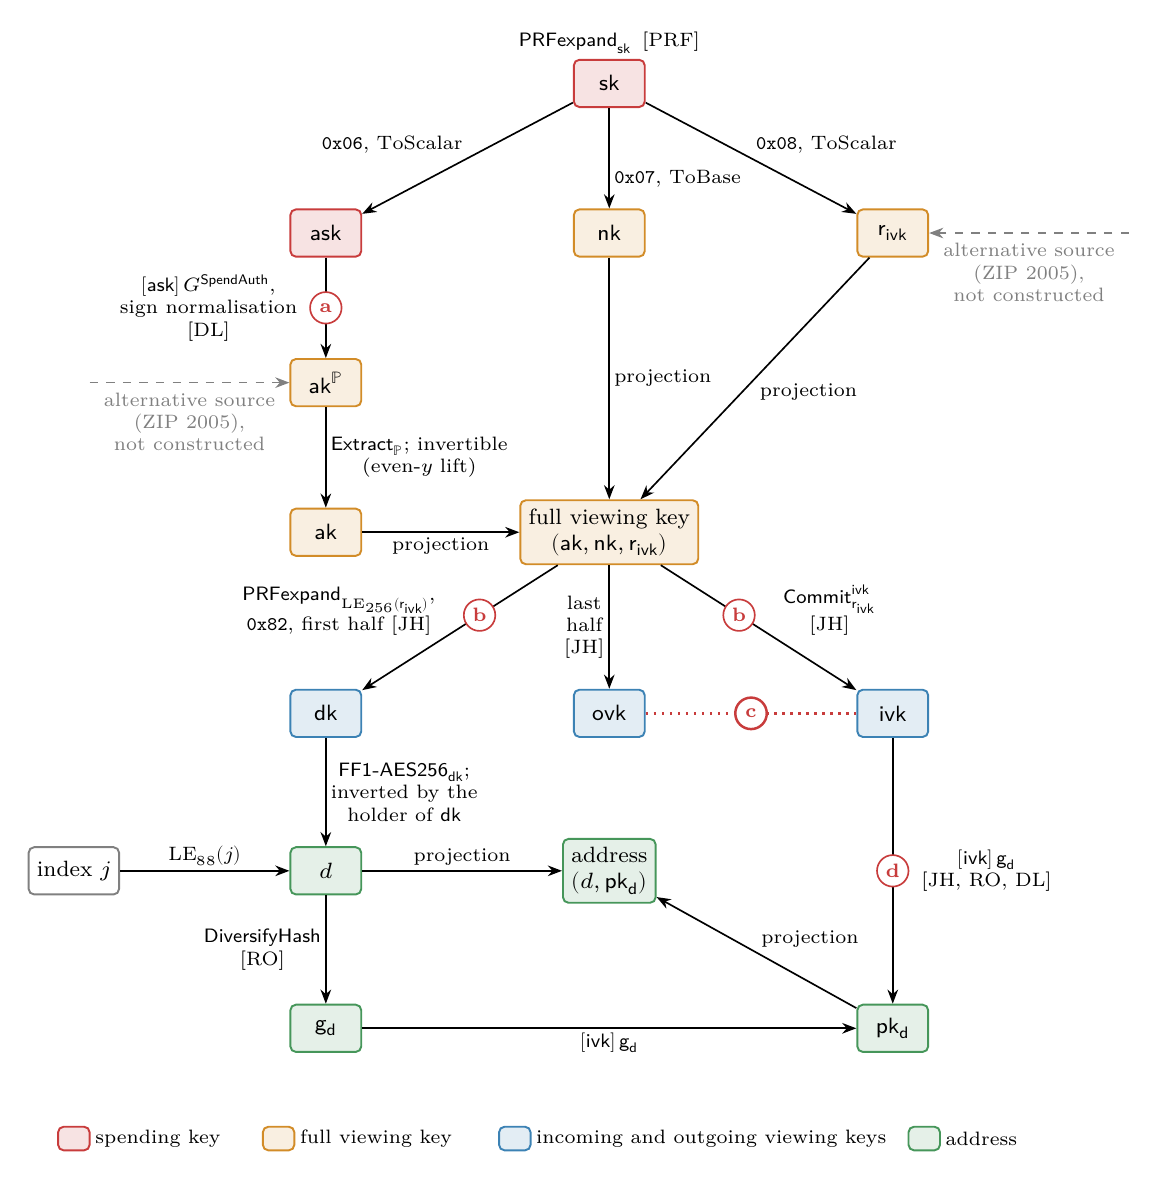
\begin{tikzpicture}[
  font=\footnotesize, >={Stealth[length=1.8mm]},
  kn/.style={draw=#1, fill=#1, fill opacity=0.14, text opacity=1,
    line width=0.7pt, rounded corners=2pt, inner sep=3pt,
    minimum height=6mm, minimum width=9mm, align=center},
  ix/.style={draw=gray, line width=0.7pt, rounded corners=2pt,
    inner sep=3pt, minimum height=6mm, minimum width=9mm},
  ed/.style={->, line width=0.6pt},
  alt/.style={->, dashed, line width=0.6pt, gray},
  lb/.style={font=\scriptsize, inner sep=1.5pt, align=center},
  mk/.style={circle, solid, draw=tierspend, fill=white, text=tierspend,
    font=\scriptsize\bfseries, inner sep=0.4pt, minimum size=4mm},
]
\node[kn=tierspend] (sk) at (6.8,0) {$\mathsf{sk}$};
\node[kn=tierspend] (ask) at (3.2,-1.9) {$\ask$};
\node[kn=tierfull] (nk) at (6.8,-1.9) {$\nksym$};
\node[kn=tierfull] (rivk) at (10.4,-1.9) {$\rivk$};
\node[kn=tierfull] (akP) at (3.2,-3.8) {$\aksym^{\PP}$};
\node[kn=tierfull] (ak) at (3.2,-5.7) {$\aksym$};
\node[kn=tierfull] (fvk) at (6.8,-5.7)
  {full viewing key\\$(\aksym, \nksym, \rivk)$};
\node[kn=tierin] (dk) at (3.2,-8.0) {$\dk$};
\node[kn=tierin] (ovk) at (6.8,-8.0) {$\ovk$};
\node[kn=tierin] (ivk) at (10.4,-8.0) {$\ivk$};
\node[ix] (j) at (0,-10.0) {index $j$};
\node[kn=tierrecv] (d) at (3.2,-10.0) {$d$};
\node[kn=tierrecv] (addr) at (6.8,-10.0) {address\\$(d, \pkd)$};
\node[kn=tierrecv] (gd) at (3.2,-12.0) {$\gd$};
\node[kn=tierrecv] (pkd) at (10.4,-12.0) {$\pkd$};
\node[lb, anchor=south] at (sk.north)
  {$\mathsf{PRFexpand}_{\mathsf{sk}}$ \,[PRF]};
\draw[ed] (sk) -- node[lb, above left]
  {$\mathtt{0x06}$, $\mathrm{ToScalar}$} (ask);
\draw[ed] (sk) -- node[lb, right, pos=0.7]
  {$\mathtt{0x07}$, $\mathrm{ToBase}$} (nk);
\draw[ed] (sk) -- node[lb, above right]
  {$\mathtt{0x08}$, $\mathrm{ToScalar}$} (rivk);
\draw[ed] (ask) -- node[mk] {a} node[lb, left=3mm]
  {$[\ask]\,G^{\mathsf{SpendAuth}}$,\\sign normalisation\\{}[DL]}
  (akP);
\draw[alt] (0.2,-3.8) -- node[lb, below=2pt, text=gray]
  {alternative source\\(ZIP 2005),\\not constructed} (akP);
\draw[alt] (13.4,-1.9) -- node[lb, below=2pt, text=gray]
  {alternative source\\(ZIP 2005),\\not constructed} (rivk);
\draw[ed] (akP) -- node[lb, right]
  {$\Extract_{\PP}$; invertible\\(even-$y$ lift)} (ak);
\draw[ed] (ak) -- node[lb, below] {projection} (fvk);
\draw[ed] (nk) -- node[lb, right] {projection} (fvk);
\draw[ed] (rivk) -- node[lb, below right] {projection} (fvk);
\draw[ed] (fvk) -- node[mk, pos=0.4] {b} node[lb, above right, pos=0.6]
  {$\CommitIvk_{\rivk}$\\{}[JH]} (ivk);
\draw[ed] (fvk) -- node[mk, pos=0.4] {b} node[lb, above left, pos=0.6]
  {$\mathsf{PRFexpand}_{\mathrm{LE}_{256}(\rivk)}$,\\
   $\mathtt{0x82}$, first half [JH]} (dk);
\draw[ed] (fvk) -- node[lb, left] {last\\half\\{}[JH]} (ovk);
\draw[dotted, line width=0.9pt, tierspend] (ovk) -- node[mk] {c} (ivk);
\draw[ed] (dk) -- node[lb, right]
  {$\mathsf{FF1\text{-}AES256}_{\dk}$;\\inverted by the\\holder of $\dk$}
  (d);
\draw[ed] (j) -- node[lb, above] {$\mathrm{LE}_{88}(j)$} (d);
\draw[ed] (d) -- node[lb, left]
  {$\mathsf{DiversifyHash}$\\{}[RO]} (gd);
\draw[ed] (d) -- node[lb, above] {projection} (addr);
\draw[ed] (ivk) -- node[mk] {d} node[lb, right=3mm]
  {$[\ivk]\,\gd$\\{}[JH, RO, DL]} (pkd);
\draw[ed] (gd) -- node[lb, below] {$[\ivk]\,\gd$} (pkd);
\draw[ed] (pkd) -- node[lb, above right] {projection} (addr);
\foreach \c/\t/\x in {tierspend/spending key/0.0,
    tierfull/full viewing key/2.6,
    tierin/incoming and outgoing viewing keys/5.6,
    tierrecv/address/10.8} {
  \node[kn=\c, minimum width=4mm, minimum height=3mm, inner sep=0pt]
    (lg) at (\x,-13.4) {};
  \node[lb, anchor=west] at (lg.east) {\t};
}
\end{tikzpicture}
\caption{Derivation graph of a key generated with
$\mathsf{use\_qsk} = \mathsf{false}$, from the spending key $\mathsf{sk}$ to
the address $(d, \pkd)$. Each edge carries its operation, and each one-way
edge also carries, in brackets, the assumption under which it is one-way:
PRF,
Assumption~\ref{ass:prf-expand}; DL, Assumption~\ref{ass:dl-pallas}; JH,
Assumption~\ref{ass:vk-hiding}; RO, Assumption~\ref{ass:grouphash-ro}. Each
one-way edge is a PRF call, a scalar multiplication, the joint hiding
assumption or $\GroupHash$ as a random oracle; bundling edges invert by
projection, $\Extract_{\PP}$ by the even-$y$ lift, and the FF1 edge is
inverted by the holder of $\dk$. The edges out of $\mathsf{sk}$ are one-way
under Assumption~\ref{ass:prf-expand}, since an algorithm recovering
$\mathsf{sk}$ from $(\ask, \nksym, \rivk)$ distinguishes
$\mathsf{PRFexpand}_{\mathsf{sk}}$ from a random function. Colours give the
lowest key tier that computes a node; the index $j$ is uncoloured. The
dashed edges into $\aksym^{\PP}$ and $\rivk$ mark the alternative source of
ZIP 2005, not constructed. Markers (a) to (d) are the four separations that
Proposition~\ref{prop:capabilities} proves; no other separation is
claimed.}
\label{fig:keys}
\end{figure}

\begin{proposition}[Capability separation]\label{prop:capabilities}
Let a key be generated honestly with $\mathsf{use\_qsk} = \mathsf{false}$.
No efficient algorithm, given the public parameters and only the listed key
material of the key, outputs the listed secret, except with negligible
probability:
\begin{enumerate}
\item[(a)] given the full viewing key $(\aksym, \nksym, \rivk)$, the scalar
  $\ask$;
\item[(b)] given the incoming viewing key $(\dk, \ivk)$, the key $\nksym$ or
  the scalar $\ask$;
\item[(c)] given $\ovk$, the scalar $\ivk$;
\item[(d)] given an address $(d, \pkd)$ of the key, the scalar $\ivk$.
\end{enumerate}
The hypotheses are: for (a), Assumptions~\ref{ass:prf-expand} (through
Lemma~\ref{lem:prf-independence}) and~\ref{ass:dl-pallas}; for (b), those of
(a) and, for $\nksym$, Assumption~\ref{ass:vk-hiding}; for (c),
Assumptions~\ref{ass:prf-expand} and~\ref{ass:vk-hiding}; for (d),
Assumptions~\ref{ass:prf-expand}, \ref{ass:vk-hiding},
\ref{ass:grouphash-ro} and~\ref{ass:dl-pallas} (``Discrete logarithms on
Pallas''). Every part also uses Lemma ``Rejection in key generation''
(\S\ref{sec:keys-viewing}), under Assumptions~\ref{ass:prf-expand},
\ref{ass:dl-pallas} and~\ref{ass:grouphash-ro}. These are the only
separations claimed.
\end{proposition}

\begin{proof}
By Lemma ``Rejection in key generation'' (\S\ref{sec:keys-viewing}), a
single draw from a uniform $\mathsf{sk}$ replaces the key at a negligible
cost. By
Lemma~\ref{lem:prf-independence}, its triple $(\ask, \nksym, \rivk)$ is
then replaced by independent uniform elements of $\F_{p_{\Vesta}}$,
$\F_{p_{\Pallas}}$ and $\F_{p_{\Vesta}}$, at a further negligible cost: in
each part the success of an algorithm is efficiently decidable from the
three values, by deriving the remaining components, running the algorithm
and comparing its output with the secret. The result is called the
idealised key.

(a)~Let an algorithm $\Adv$ output $\ask$ from $(\aksym, \nksym, \rivk)$
with probability $\epsilon$ for the idealised key. An algorithm $\mathcal{B}$
receives $Y = [s]\,G^{\mathsf{SpendAuth}}$ for $s$ uniform on
$\F_{p_{\Vesta}}$, draws $\nksym$ and $\rivk$ uniformly, and runs $\Adv$ on
$(\Extract_{\PP}(Y), \nksym, \rivk)$. The input is distributed as for the
idealised key, because the sign normalisation replaces $\ask$ by $\pm\ask$
and does not change $\aksym$ (Lemma~\ref{lem:opposite-points}). A correct
output $a$ satisfies $[a]\,G^{\mathsf{SpendAuth}} = \aksym^{\PP}$, the
even-$y$ lift of $\Extract_{\PP}(Y)$, which is $Y$ or $-Y$; $\mathcal{B}$
outputs whichever of $a$ and $-a$ maps to $Y$. Hence $\mathcal{B}$ computes
discrete logarithms to the generator $G^{\mathsf{SpendAuth}}$ with
probability $\epsilon$, and $\epsilon$ is negligible by
Assumption~\ref{ass:dl-pallas}.

(b)~An algorithm that computes $\ask$ from $(\dk, \ivk)$ computes it from
$(\aksym, \nksym, \rivk)$ by first deriving $(\dk, \ivk)$, so (a) applies.
Let $\Adv$ output $\nksym$ from $(\dk, \ivk)$ with probability $\epsilon$. A
distinguisher for Assumption~\ref{ass:vk-hiding}, given
$(\aksym, \nksym)$ of the idealised key and a triple $(x, y, z)$, runs $\Adv$
on $(y, x)$ and outputs $1$ exactly when $\Adv$ outputs $\nksym$. On the
real triple it outputs $1$ with probability $\epsilon$. On the ideal triple
$\Adv$ receives $u_1$ and $\CommitIvk_{\rivk'}(\aksym, \nksym)$, which is
independent of $\nksym$ unless $\hat{M} = \bot$, a negligible event
(Lemma ``Rejection in key generation''); since $\nksym$ is uniform on
$\F_{p_{\Pallas}}$, $\Adv$ then succeeds with probability at most
$1/p_{\Pallas}$ plus a negligible term. So $\epsilon$ exceeds the
distinguisher's advantage by a negligible amount at most.

(c)~Let $\Adv$ output $\ivk$ from $\ovk$ with probability $\epsilon$. The
distinguisher given $(\aksym, \nksym)$ and $(x, y, z)$ runs $\Adv$ on $z$
and outputs $1$ exactly when $\Adv$ outputs $x$. On the ideal triple, $z =
u_2$ is independent of $x = \CommitIvk_{\rivk'}(\aksym, \nksym)$, which, for
$\hat{M} \neq \bot$, takes each value with probability at most
$2/p_{\Vesta}$ by Lemma ``Distribution of $\ivk$''. Hence $\epsilon$ is at most
the advantage under Assumption~\ref{ass:vk-hiding} plus $2/p_{\Vesta}$ and
a negligible term.

% compute/fields.py:
% [sec:keys-capabilities] uniform exponent mod p_Vesta lies in that set
%   with probability (p_Vesta - 1)/(2 p_Vesta) = 1/2 - 1/(2 p_Vesta);
%   loss factor 2 p_Vesta/(p_Vesta - 1) = 2 + 2/(p_Vesta - 1)
(d)~Let $\Adv$ output $\ivk$ from the address at an index $j$, possibly of
its choice, with probability $\epsilon$. The distinguisher given
$(\aksym, \nksym)$ and $(x, y, z)$ computes
$d := \mathsf{FF1\text{-}AES256}_{y}(\mathrm{LE}_{88}(j))$,
$\gd := \mathsf{DiversifyHash}(d)$ and $\pkd := [x]\,\gd$, runs $\Adv$ on
$(d, \pkd)$, and outputs $1$ exactly when $\Adv$ outputs $x$. On the ideal
triple, $\Adv$ succeeds with probability $\epsilon' \geq \epsilon - \delta$,
for $\delta$ the advantage under Assumption~\ref{ass:vk-hiding}; there,
outside the negligible event $\hat{M} = \bot$, the value $\ivk := x$ is $0$
with probability $1/p_{\Vesta}$ and otherwise uniform on $X_{\Pallas}$,
independently of $(\aksym, \nksym)$ and of $u_1$, hence of $d$. An
algorithm $\mathcal{B}$ receives a generator $G$ and $Y = [s]\,G$ for $s$
uniform on $\F_{p_{\Vesta}}$. It draws $t$ uniform on
$\F_{p_{\Vesta}} \setminus \{0\}$ and $u_1$ uniform, computes $d$ from
$u_1$ and $j$, programs $\GroupHash$ at
$(\texttt{z.cash:Orchard-gd}, \mathsf{LEBS2OSP}_{88}(d))$ with the uniform
non-identity point $[t]\,G$ (Assumption~\ref{ass:grouphash-ro}), answers
other queries with fresh uniform points, and runs $\Adv$ on
$(d, [t]\,Y) = (d, [s]([t]\,G))$. With probability
$(p_{\Vesta} - 1)/(2 p_{\Vesta})$ the exponent $s$ lies in $X_{\Pallas}$;
it is then uniform on $X_{\Pallas}$, and the view of $\Adv$ is that of the
ideal triple conditioned on $\ivk \neq 0$, up to statistical distance
$1/p_{\Vesta}$ for the programmed point. Algorithm $\mathcal{B}$ outputs the
output of $\Adv$ and so computes $s$ with probability at least
\[
  \frac{p_{\Vesta} - 1}{2 p_{\Vesta}}
  \Bigl(\epsilon' - \frac{2}{p_{\Vesta}}\Bigr),
\]
a loss factor of $2 p_{\Vesta}/(p_{\Vesta} - 1)$, about $2$, against
Assumption~\ref{ass:dl-pallas}. Hence $\epsilon'$, and with it $\epsilon$,
is negligible.
\end{proof}

Of the objects of this section only an address $(d, \pkd)$, with the base
$\gd$ computed from $d$, is public; $\mathsf{sk}$, $\ask$, $\aksym^{\PP}$,
$\aksym$, $\nksym$, $\rivk$, the full viewing key, $\dk$, $\ivk$, $\ovk$ and
the index $j$ are secret key material. One incoming viewing key yields
$2^{88}$ addresses (\S\ref{sec:keys-addr}), unlinkable in the sense of
Proposition~\ref{prop:addr-unlinkable} (``Unlinkability of diversified
addresses'').

What a holder of each key can compute from the objects of later sections is
stated where those objects are constructed, each with a back-reference to
Proposition~\ref{prop:capabilities}: from nullifiers in ``Nullifier
uniqueness and unlinkability'' (\S\ref{sec:nf-props}), and from note
ciphertexts in ``The outgoing ciphertext'' (\S\ref{sec:enc-out}) and ``Trial
decryption and note acceptance'' (\S\ref{sec:enc-trial}). This section states
no such power.

Keys and addresses are objects of the Orchard protocol, not of a pool: one
key hierarchy and one address format serve both the Orchard pool and the
Ironwood pool (ZIP 229, Abstract).

\section{Notes and note commitments}\label{sec:notes}

This section defines the note, its commitment and its extracted commitment,
and proves their hiding and binding; it constructs the derivation of all
randomness of a created note from one seed under the lead byte
$\mathtt{0x03}$, and defines the Action and the bundle as units of a
transaction.

\subsection{Notes}\label{sec:notes-note}

\begin{definition}[Unit of value]
The \emph{zatoshi} is the smallest unit of value; one ZEC, the unit of the
native currency of Zcash, is $10^8$ zatoshi (protocol specification,
\href{https://zips.z.cash/protocol/protocol.pdf#notes}%
{\S``Shielded Pools and Notes''} and
\href{https://zips.z.cash/protocol/protocol.pdf#networks}%
{\S``Mainnet and Testnet''}). Every value in this volume, note values
included, is an integer number of zatoshi.
\end{definition}

\begin{definition}[Note]
A \emph{note} is a tuple $n = (\mathsf{addr}, v, \rho, \psi, \rcm)$, where
\begin{itemize}
\item the address $\mathsf{addr} = (d, \pkd)$ of the recipient, of the type
  constructed in \S\ref{sec:keys-addr}: a diversifier $d \in \{0,1\}^{88}$
  and a transmission key
  $\pkd \in \Ep(\F_{p_{\Pallas}}) \setminus \{\mathcal{O}\}$;
\item the value $v \in \{0, \dots, 2^{64} - 1\}$, in zatoshi;
\item the elements $\rho \in \F_{p_{\Pallas}}$ and
  $\psi \in \F_{p_{\Pallas}}$;
\item the commitment trapdoor $\rcm \in \F_{p_{\Vesta}}$
\end{itemize}
(protocol specification, \S``Shielded Pools and Notes''; the lengths $88$
and $64$ are those of \S``Constants''). The specification types $\rcm$ as an
integer in $\{0, \dots, 2^{255} - 1\}$ (\S``Commitment''). This volume types
it in $\F_{p_{\Vesta}}$, because every derivation of $\rcm$ yields a reduced
value and $\rcm$ acts only as the scalar of $[\rcm]$, which depends on $\rcm$
modulo $p_{\Vesta}$ alone; this typing makes the binding of
Proposition~\ref{prop:cm} a statement about notes. For a created note, $\psi$
and $\rcm$ are derived from its note seed, for an Ironwood-pool note in
\S\ref{sec:notes-seed}, and $\rho$ is the nullifier of the note consumed in
the same Action, a rule constructed in ``Nullifier chaining''
(\S\ref{sec:nf-chaining}).
\end{definition}

A note is never published. A transaction that creates a note publishes its
extracted note commitment $\cmx$ (Definition~\ref{def:notecommit}) and a
ciphertext of its note plaintext for the recipient, constructed in
``Encryption to the recipient'' (\S\ref{sec:enc-encrypt}) (protocol
specification, \S``Note Commitments'' and \S``Sending Notes (Orchard)''). Of
the fields of a created note, only $\rho$ appears on chain in the clear: it
equals the nullifier that the same Action publishes for its consumed note
(``Nullifier chaining'', \S\ref{sec:nf-chaining}). This representation of
value serves requirement R1 of \S\ref{sec:intro-req};
Propositions~\ref{prop:cm} and~\ref{prop:cm-derived} state what the
commitment hides.

\begin{remark}[Roles of the fields]
The address and the value are the content of the note, its recipient and
its amount; the trapdoor $\rcm$ randomises its commitment; the elements
$\rho$ and $\psi$, which also enter the commitment, are the note-specific
inputs of its nullifier, constructed in ``The nullifier''
(\S\ref{sec:nf-nullifier}).
\end{remark}

\subsection{Note commitments}\label{sec:notes-cm}

% compute/encodings.py:
% [sec:prim-sinsemilla] NoteCommit (g_d* || pk_d* || LE_64(v) || LE_255(rho)
%   || LE_255(psi)): 1086 bits, 109 chunks of 10 bits (padding 4); <= c = 253
\begin{definition}[Note commitment]\label{def:notecommit}
For a note $n = ((d, \pkd), v, \rho, \psi, \rcm)$ let
$\gd := \mathsf{DiversifyHash}(d)$ (\S\ref{sec:keys-addr}) and
\[
  M(n) := \gd^{\star} \,\|\, \pkd^{\star} \,\|\, \mathrm{LE}_{64}(v)
    \,\|\, \mathrm{LE}_{255}(\rho) \,\|\, \mathrm{LE}_{255}(\psi),
\]
with $\rho$ and $\psi$ read as integers in $\{0, \dots, p_{\Pallas} - 1\}$;
the string $M(n)$ has the fixed length $1086$ of
Table~\ref{tab:prim-sinsemilla}. With
$D := \texttt{z.cash:Orchard-NoteCommit}$, the \emph{note commitment} of $n$
is
\[
  \cmsym := \NoteCommit_{\rcm}(M(n))
    := \mathsf{SinsemillaCommit}_{\rcm}(D, M(n))
    \in \Ep(\F_{p_{\Pallas}}) \cup \{\bot\}.
\]
By the routing of \S\ref{sec:prim-sinsemilla}, with the hash point and the
blinding base
\begin{align*}
  \hat{M} &:= \mathsf{SinsemillaHashToPoint}(
    \texttt{z.cash:Orchard-NoteCommit-M},\, M(n)), \\
  H_D &:= \GroupHash(\texttt{z.cash:Orchard-NoteCommit-r},\, \varepsilon),
\end{align*}
the commitment is $\cmsym = \hat{M} + [\rcm]\,H_D$ if $\hat{M} \neq \bot$,
and $\cmsym = \bot$ otherwise. The \emph{extracted note commitment} is
$\cmx := \Extract_{\PP}^{\bot}(\cmsym) \in \F_{p_{\Pallas}} \cup \{\bot\}$
(\S\ref{sec:prim-fields}). The specification's $\NoteCommit$ takes the five
encoded fields as separate arguments, in the order of their encodings in
$M(n)$ (protocol specification, \S``Sinsemilla commitments'', \S``Sending
Notes (Orchard)'' and \S``Coordinate Extractor for Pallas'').
\end{definition}

A sender never publishes $\bot$: it redraws the note seed (step~(vi) of the
derivation of \S\ref{sec:notes-seed}). The extracted commitment $\cmx$ is the
value an Action publishes for its created note, and the leaf of that note in
the pool's note commitment tree of ``The Merkle hash and the tree''
(\S\ref{sec:tree-hash}), whose nodes are elements of $\F_{p_{\Pallas}}$.

The blinding base $H_D$ is not $\mathcal{O}$: the protocol specification,
\S``Sinsemilla commitments'', states that $\mathsf{SinsemillaCommit}$ is
perfectly hiding for a uniform trapdoor, for every domain, which holds only
for a blinding base other than $\mathcal{O}$ (as for $\CommitIvk$,
\S\ref{sec:keys-viewing}).

% compute/fields.py:
% [sec:prim-fields] bit length of p_Pallas = 255, of p_Vesta = 255;
%   p_Pallas < p_Vesta
\begin{proposition}[Hiding and binding of note commitments]\label{prop:cm}
\leavevmode
\begin{enumerate}
\item[(a)] Perfect hiding. Let $\rcm$ be uniform on $\F_{p_{\Vesta}}$. For
  every note content $(d, \pkd, v, \rho, \psi)$ whose message $M(n)$ has hash
  point $\hat{M} \neq \bot$, the commitment $\cmsym$ is uniform on
  $\Ep(\F_{p_{\Pallas}})$. Hence the distributions of $\cmsym$ and of $\cmx$
  do not depend on $(\gd, \pkd, v, \rho, \psi)$, and $\NoteCommit$ is
  perfectly hiding on messages without a $\bot$ output, in the sense of the
  \emph{Crypto Guide}'s Definition ``Hiding game and hiding''
  (\S``Hiding and binding'').
\item[(b)] Binding of the extracted commitment. Under
  Assumptions~\ref{ass:dl-pallas} and~\ref{ass:grouphash-ro}, no efficient
  algorithm outputs, except with negligible probability, two notes
  $n \neq n'$ with $\cmx(n) = \cmx(n') \neq \bot$. In particular two
  distinct notes share no note commitment other than $\bot$. With
  Proposition~\ref{prop:sinsemilla-cr}(iii), which excludes messages with
  output $\bot$, part~(b) gives computational binding in the sense of the
  \emph{Crypto Guide}'s Definition ``Binding game and binding'' (same
  section), with the note content as the message and $\rcm$ as the
  randomness, stated for notes and for the extracted value.
\end{enumerate}
Proposition~\ref{prop:cm-derived} states hiding for the trapdoor that a
sender derives.
\end{proposition}

\begin{proof}
(a)~This is Lemma~\ref{lem:sinsemilla-commit}(i) for the domain $D$ and the
message length $1086$, whose hypothesis $H_D \neq \mathcal{O}$ holds by the
paragraph above; the value $\cmx$ is a fixed function of $\cmsym$. Equal
distributions for every pair of contents without a $\bot$ output are perfect
hiding by the
\emph{Crypto Guide}'s Proposition ``Distributional characterisation of
hiding'' (\S``Hiding and binding'').

(b)~Step~1 reduces distinct notes to distinct openings. The map
$(\gd, \pkd, v, \rho, \psi) \mapsto M(n)$ is injective: the string $M(n)$
concatenates fields of fixed lengths; the star encoding is injective
(\S\ref{sec:prim-fields}); the encoding $\mathrm{LE}_{64}$ is injective on
$\{0, \dots, 2^{64} - 1\}$; and the encoding $\mathrm{LE}_{255}$ is injective
on the representatives of $\F_{p_{\Pallas}}$, since $p_{\Pallas} < 2^{255}$
(\S\ref{sec:prim-fields}). The map $n \mapsto (M(n), \rcm)$ is therefore
injective except on pairs of notes
with $d \neq d'$ and $\mathsf{DiversifyHash}(d) =
\mathsf{DiversifyHash}(d')$. Let $T$ and $T'$ be the values of $\GroupHash$ at
$(\texttt{z.cash:Orchard-gd}, \mathsf{LEBS2OSP}_{88}(d))$ and at the
corresponding input for $d'$, distinct inputs because
$\mathsf{LEBS2OSP}_{88}$ is injective. If $T, T' \neq \mathcal{O}$, equal
diversified bases give $T - T' = \mathcal{O}$; otherwise $T = \mathcal{O}$
or $T' = \mathcal{O}$. Each is a non-trivial relation among values of
$\GroupHash$ on distinct inputs, which the lemma on relations among fixed
generators (\S\ref{sec:prim-sinsemilla}) excludes except with negligible
probability.

Step~2 treats distinct openings. Let $\cmx(n) = \cmx(n') \neq \bot$. The
lifting $\Extract_{\PP}^{\bot}$ maps only $\bot$ to $\bot$, so $\cmsym$ and
$\cmsym'$ are points, and by Lemma~\ref{lem:opposite-points}
$\cmsym' = \cmsym$ or $\cmsym' = -\cmsym$. The pairs $(M(n), \rcm)$ and
$(M(n'), \rcm')$ are openings of the instance $\NoteCommit$ in
$\{0,1\}^{1086} \times \F_{p_{\Vesta}}$. By
Proposition~\ref{prop:sinsemilla-cr}(ii), outputs with $\cmsym' = -\cmsym$,
or with $\cmsym' = \cmsym$ and $M(n) \neq M(n')$, have negligible
probability (in the opposite case the relation in its proof has
coefficient $2^{109 + 1}$ on the hash base, for a message of $109$ chunks).
In the remaining case $\cmsym' = \cmsym$ and $M(n) = M(n')$, and outside the
event of Step~1 the openings differ, so $\rcm \neq \rcm'$ in
$\F_{p_{\Vesta}}$; then $[\rcm - \rcm']\,H_D = \mathcal{O}$, impossible for
$H_D \neq \mathcal{O}$ in a group of prime order $p_{\Vesta}$. A note
commitment other than $\bot$ shared by $n \neq n'$ gives equal extracted
commitments other than $\bot$, which proves the particular case.
\end{proof}

\subsection{The note seed: Ironwood derivations (lead byte
\texorpdfstring{$\mathtt{0x03}$}{0x03})}\label{sec:notes-seed}

\begin{definition}[Note seed and lead byte]
A created note reaches its recipient as a \emph{note plaintext}, the byte
string constructed in ``The note plaintext'' (\S\ref{sec:enc-plaintext}) that
the sender encrypts. Its first byte, the \emph{lead byte}, names the format
of the plaintext and selects the derivation of the note's randomness. The
sender draws one \emph{note seed} $\mathsf{rseed}$, a uniform $32$-byte
string, the key type of $\mathsf{PRFexpand}$ (\S\ref{sec:prim-prf}), which
the plaintext carries. The values $\psi$ and $\rcm$ of the note and the
ephemeral secret key $\mathsf{esk} \in \F_{p_{\Vesta}}$ of ``Encryption to
the recipient'' (\S\ref{sec:enc-encrypt}) are all derived from it (protocol
specification, \S``Note Plaintexts and Memo Fields'' and \S``Sending Notes
(Orchard)'').
\end{definition}

% compute/encodings.py:
% [sec:notes-seed] pre_rcm = 1 + 32 + 32 + 8 + 32 + 32 = 137 bytes
\begin{construction}[Derivations under lead byte $\mathtt{0x03}$]
The input is an address $(d, \pkd)$, a value $v \in \{0, \dots, 2^{64} - 1\}$
and $\rho \in \F_{p_{\Pallas}}$. Let $\gd := \mathsf{DiversifyHash}(d)$ and
$\underline{\rho} := \mathsf{I2LEOSP}_{256}(\rho)$. For a point $P = (x, y)$
the $32$-byte string $\mathsf{LEBS2OSP}_{256}(P^{\star})$ equals
$\mathsf{I2LEOSP}_{256}(x + 2^{255} (y \bmod 2))$ (\S\ref{sec:prim-fields}).
The sender
\begin{enumerate}[label=(\roman*)]
\item checks that $\pkd \neq \mathcal{O}$;
\item draws $\mathsf{rseed}$ uniformly from the $32$-byte strings;
\item derives
  $\mathsf{esk} := \mathrm{ToScalar}\bigl(\mathsf{PRFexpand}_{\mathsf{rseed}}
  ([\mathtt{0x04}] \,\|\, \underline{\rho})\bigr) \in \F_{p_{\Vesta}}$,
  and returns to~(ii) if $\mathsf{esk} = 0$;
\item derives
  $\psi := \mathrm{ToBase}\bigl(\mathsf{PRFexpand}_{\mathsf{rseed}}
  ([\mathtt{0x09}] \,\|\, \underline{\rho})\bigr) \in \F_{p_{\Pallas}}$;
\item derives
  $\rcm := \mathrm{ToScalar}\bigl(\mathsf{PRFexpand}_{\mathsf{rseed}}
  (\mathsf{pre\_rcm})\bigr) \in \F_{p_{\Vesta}}$, where
  \begin{align*}
    \mathsf{pre\_rcm} := [\mathtt{0x0B}]
      &\,\|\, \mathsf{LEBS2OSP}_{256}(\gd^{\star})
      \,\|\, \mathsf{LEBS2OSP}_{256}(\pkd^{\star}) \\
      &\,\|\, \mathsf{I2LEOSP}_{64}(v) \,\|\, \underline{\rho}
      \,\|\, \mathsf{I2LEOSP}_{256}(\psi),
  \end{align*}
  a string of $1 + 32 + 32 + 8 + 32 + 32 = 137$ bytes;
\item computes $\cmx$ of the note $n := ((d, \pkd), v, \rho, \psi, \rcm)$ by
  Definition~\ref{def:notecommit}, and returns to~(ii) if $\cmx = \bot$.
\end{enumerate}
The output is the note $n$, its seed $\mathsf{rseed}$ and $\mathsf{esk}$
(protocol specification, \S``Sending Notes (Orchard)''; ZIP 2005,
``Changes to the Protocol Specification'', \S 4.7.3).
\end{construction}

The order is forced: the string $\mathsf{pre\_rcm}$ contains $\psi$, so
$\rcm$ is derived after $\psi$. The strings $\gd^{\star}$ and $\pkd^{\star}$ in
$\mathsf{pre\_rcm}$ are those of the message $M(n)$, packed into bytes, so
$\rcm$ is a function of $\mathsf{rseed}$ and of every committed field
$(\gd, \pkd, v, \rho, \psi)$. The leading bytes $\mathtt{0x04}$,
$\mathtt{0x09}$ and $\mathtt{0x0B}$ are rows of
Table~\ref{tab:prim-prf}.

An Ironwood-pool note has the type of Definition ``Note''
(\S\ref{sec:notes-note}) and is committed by the same $\NoteCommit$
(Definition~\ref{def:notecommit}). Every note created by an Ironwood-pool
Action, a dummy created note included, has a plaintext with lead byte
$\mathtt{0x03}$ and the derivations above; no note created by an
Orchard-pool Action does. This is the only note-level distinction between the
two pools (ZIP 229, ``Transaction Format''; ZIP 258, ``ZIP 2005
activation'').

% compute/fields.py:
% [sec:prim-prf] ToScalar (mod p_Vesta): Math Guide bound m/2^512
%   = 2^-258 (1 + e), 0 < e < 2^-128, so < 2^-257;
%   exact distance t(m-t)/(m 2^512) = 2^-260.99
\begin{proposition}[Hiding under the derived trapdoor]%
\label{prop:cm-derived}
An adversary chooses two tuples $(d^{(i)}, \pkd^{(i)}, v^{(i)}, \rho^{(i)})$,
$i \in \{0, 1\}$, of the input type of the construction above, with
$\pkd^{(i)} \neq \mathcal{O}$. The challenger draws a uniform bit $b$, runs
steps (ii) to (vi) of the construction on tuple~$b$, and returns
$(\cmsym_b, \mathsf{esk}_b)$, the note commitment of the note it computes
and its $\mathsf{esk}$; the adversary receives no other function of
$\mathsf{rseed}$ (the ciphertext that carries $\mathsf{rseed}$ is treated in
Theorem~\ref{thm:privacy}). It outputs a bit $b'$. Let the number
$\epsilon_{\mathsf{PRF}}$ bound the advantage against
Assumption~\ref{ass:prf-expand} of each algorithm built from the adversary in
the proof, each of which queries $\mathsf{PRFexpand}_{\mathsf{rseed}}$ on
three inputs with pairwise distinct leading bytes; let $\delta < 2^{-257}$
bound the distance of $\mathrm{ToScalar}$ from uniform
(\S\ref{sec:prim-prf}); and let $\epsilon_{\bot}$ be the largest, over $i$,
of the sum of two probabilities that one pass through steps (ii) to (vi) on
tuple~$i$ returns to step~(ii), one with $\mathsf{PRFexpand}_{\mathsf{rseed}}$
as specified and one with its three outputs replaced by independent uniform
strings. Then
\[
  \bigl|\Pr[b' = 1 \mid b = 0] - \Pr[b' = 1 \mid b = 1]\bigr|
  \le 2\,(\epsilon_{\mathsf{PRF}} + \delta + \epsilon_{\bot}),
\]
and $\epsilon_{\mathsf{PRF}}$ and $\epsilon_{\bot}$ are negligible under
Assumptions~\ref{ass:prf-expand}, \ref{ass:dl-pallas}
and~\ref{ass:grouphash-ro}. The same bound holds with $\cmx_b$ in place of
$\cmsym_b$.
\end{proposition}

\begin{proof}
Fix the adversary's tuples. One pass through steps (ii) to (vi) with a
fresh $\mathsf{rseed}$ is a \emph{trial}; its output is
$(\cmsym, \mathsf{esk})$, and it is \emph{accepted}, event $A$, when
$\mathsf{esk} \neq 0$ and $\hat{M} \neq \bot$, since $\cmx = \bot$ exactly
when $\hat{M} = \bot$. Trials are independent and identically distributed,
and the challenger returns the output of the first accepted one; so its
answer $X_i$ on tuple~$i$ is distributed as the output $Y_i$ of one trial
conditioned on $A$. For a random variable $Y$ and an event $A$ with
$\Pr[\neg A] = p < 1$, the statistical distance between $Y$ and $Y$
conditioned on $A$ is at most $p$: for every set $S$,
\[
  \Pr[Y \in S] - \Pr[Y \in S \mid A]
  = \Pr[Y \in S,\, \neg A]
    - \Pr[Y \in S,\, A]\,\frac{p}{1 - p},
\]
and both terms lie in $[0, p]$.

Hybrid~1 replaces the outputs of $\mathsf{PRFexpand}_{\mathsf{rseed}}$ on
$[\mathtt{0x04}] \,\|\, \underline{\rho}$,
$[\mathtt{0x09}] \,\|\, \underline{\rho}$ and $\mathsf{pre\_rcm}$ by
independent uniform $u_1, u_2, u_3 \in \{0,1\}^{512}$, so that
$\mathsf{esk} = \mathrm{ToScalar}(u_1)$, $\psi = \mathrm{ToBase}(u_2)$ and
$\rcm = \mathrm{ToScalar}(u_3)$. The three inputs have distinct leading
bytes, the input $\mathsf{pre\_rcm}$ is chosen after the answer that
determines $\psi$, and $\mathsf{rseed}$ is used only as a key of
$\mathsf{PRFexpand}$. By Lemma~\ref{lem:prf-independence}
(Assumption~\ref{ass:prf-expand}), the probability that any efficient test
outputs $1$ on the trial's output changes by at most
$\epsilon_{\mathsf{PRF}}$.
Hybrid~2 replaces $\rcm$ by a uniform element of $\F_{p_{\Vesta}}$,
independent of all else, at statistical cost $\delta$. The event $A$ does
not involve $\rcm$, so its probability is the same in both hybrids.

In Hybrid~2 the values $\mathsf{esk}$ and $\psi$ are independent, $A$ is the
intersection of an event on $\mathsf{esk}$ and an event on $\psi$, and
$\rcm$ is uniform and independent of both. Conditioned on $A$, therefore,
$\hat{M} \neq \bot$ and $\cmsym = \hat{M} + [\rcm]\,H_D$ is uniform on
$\Ep(\F_{p_{\Pallas}})$ by Proposition~\ref{prop:cm}(a), independently of
$\mathsf{esk}$, and $\mathsf{esk}$ is distributed as $\mathrm{ToScalar}(u_1)$
conditioned on being non-zero. This distribution $W$ does not depend on $i$.

For each $i$, the adversary's output probability on $X_i$ differs from that
on $W$ by at most the rejection probability of a trial as specified ($X_i$
against $Y_i$), plus $\epsilon_{\mathsf{PRF}} + \delta$ ($Y_i$ against its
form in Hybrid~2), plus the rejection probability in Hybrid~2, which equals
that with uniform strings (the unconditioned form in Hybrid~2 against $W$).
The two rejection probabilities sum to at most $\epsilon_{\bot}$. Adding the
bounds for $i = 0$ and $i = 1$ gives the stated bound. For $\cmx_b$, an
adversary against $\cmx_b$ is one against $\cmsym_b$ that first applies the
fixed map $\Extract_{\PP}^{\bot}$.

Negligibility. With uniform strings, $\mathsf{esk} = 0$ has probability at
most $1/p_{\Vesta} + \delta$. The event $\hat{M} = \bot$ has the probability
with which an efficient algorithm finds a message of hash point $\bot$: the
algorithm that runs the adversary's choice of tuples, draws $u_2$, and
outputs $M(n)$ for tuple~$i$ with $\psi = \mathrm{ToBase}(u_2)$. That
probability is negligible by
Proposition~\ref{prop:sinsemilla-cr}(iii) under
Assumptions~\ref{ass:dl-pallas} and~\ref{ass:grouphash-ro}. Rejection is
efficiently decidable from the three outputs of
$\mathsf{PRFexpand}_{\mathsf{rseed}}$, so the rejection probability as
specified exceeds that with uniform strings by at most
$\epsilon_{\mathsf{PRF}}$, negligible under
Assumption~\ref{ass:prf-expand}.
\end{proof}

\begin{remark}[Purpose of the hashed trapdoor]
Because $\rcm$ is a hash of $\mathsf{rseed}$ and of every committed field,
Ironwood-pool notes are recoverable in the sense of ZIP 2005. That ZIP
proposes, with details subject to change, a Recovery Protocol for recovering
Ironwood-pool funds if the Orchard protocol must be disabled because
discrete logarithms become computable; a recovery protocol whose statement
recomputes $\rcm$ by this derivation can bind a note even against an
adversary able to compute discrete logarithms (ZIP 2005, Abstract;
Rationale, ``Proposed Recovery Protocol'' and ``Repairing note
commitments''). Against such an adversary $\NoteCommit$ alone is not
binding: the discrete-logarithm relations between its bases give a linear
equation over $\F_{p_{\Vesta}}$ with several solutions, hence two distinct
notes that open one commitment (ZIP 2005, Rationale, ``Attacks against
binding of note commitments''). What the deployed protocol checks of the
derivation is stated with the Action statement, defined in ``The Action
statement'' (\S\ref{sec:action-statement}).
\end{remark}

The specification defines, for each pool, the set
$\mathsf{allowedLeadBytes}^{\mathit{pool}}$ of lead bytes allowed in a note
plaintext of that pool. For every transaction that contains Actions of the
pool, the set is $\{\mathtt{0x03}\}$ for the Ironwood pool and
$\{\mathtt{0x02}\}$ for the Orchard pool (protocol specification, \S``Note
Plaintexts and Memo Fields''; ZIP 2005, ``Changes to the Protocol
Specification'', \S 3.2.1; ZIP 258, ``ZIP 2005 activation''). The lead byte
travels encrypted, and each decrypting party enforces the rule: decryption
with an incoming viewing key, by the recipient, and decryption with an
outgoing viewing key, by its holder, both return $\bot$ when the lead byte is
not allowed
(\href{https://zips.z.cash/protocol/protocol.pdf#decryptivk}%
{\S``Decryption using an Incoming Viewing Key (Sapling and Orchard)''} and
\href{https://zips.z.cash/protocol/protocol.pdf#decryptovk}%
{\S``Decryption using an Outgoing Viewing Key (Sapling and Orchard)''}).
For an Ironwood-pool output this is check~(i) of the acceptance
procedure of ``Trial decryption and note acceptance''
(\S\ref{sec:enc-trial}). The one consensus check of the lead byte is stated
in ``Chain state and pool rules'' (\S\ref{sec:tx-pools}).

\subsection{Actions, bundles, and dummy notes}\label{sec:notes-action}

\begin{definition}[Action]
An \emph{Action} of a pool consumes one note $n^{\mathsf{old}}$ and creates
one note $n^{\mathsf{new}}$ of that pool; it is the specification's Action
transfer, and every Action has both sides (protocol specification,
\S``Action Transfers and their Descriptions''). Its public data carry the
extracted commitment $\cmx$ of the created note
(Definition~\ref{def:notecommit}), the nullifier of the consumed note
(``The nullifier'', \S\ref{sec:nf-nullifier}), a randomised validating key
with a spend-authorisation signature (``Randomised validating keys'',
\S\ref{sec:spendauth-rk}), a net value commitment (``Value commitments'',
\S\ref{sec:value-cv}), and the ciphertexts of ``Encryption to the
recipient'' (\S\ref{sec:enc-encrypt}). ``Action descriptions and bundles''
(\S\ref{sec:tx-bundle}) assembles them and redefines neither the Action nor
the bundle. The relation that each Action must satisfy is the Action
statement, defined in ``The Action statement''
(\S\ref{sec:action-statement}).
\end{definition}

\begin{definition}[Dummy notes]
Every Action has one consumed and one created note, so that its public
fields are the same whether a side is real or not; a side that a payment
does not use carries a \emph{dummy note}, a note of value $0$. A
\emph{dummy consumed note} is built as follows (protocol specification,
\S``Dummy Notes (Orchard)''; ZIP 2005, ``Changes to the Protocol
Specification'', \S 4.8.3):
\begin{enumerate}[label=(\roman*)]
\item draw a fresh spending key as in \S\ref{sec:keys-sk}, and derive its
  key components and an address $(d, \pkd)$ (\S\ref{sec:keys-viewing},
  \S\ref{sec:keys-addr});
\item set $v := 0$, draw $\mathsf{rseed}$ uniformly, and set
  $\rho := \Extract_{\PP}(P)$ for a uniform point $P$ of
  $\Ep(\F_{p_{\Pallas}})$;
\item derive $\psi$ and $\rcm$ under the lead byte chosen as for a created
  note of the pool (ZIP 2005, ``Changes to the Protocol Specification'',
  \S 4.8.3); in the Ironwood pool the lead byte is $\mathtt{0x03}$ and the
  derivations are steps (iv) and~(v) of \S\ref{sec:notes-seed};
\item compute $\cmsym$ by Definition~\ref{def:notecommit}, and repeat from
  the draw of $\mathsf{rseed}$ with a fresh seed if $\cmsym = \bot$.
\end{enumerate}
Its nullifier is computed as for any note (``The nullifier'',
\S\ref{sec:nf-nullifier}). For step~(iii) the two sources differ: the
specification's section chooses the lead byte with the pool fixed to the
Orchard pool, which gives $\mathtt{0x02}$ also in the Ironwood pool, whereas
ZIP 2005, \S 4.8.3, makes the choice identical for dummy and non-dummy
notes. The volume follows the ZIP. No condition of the Action statement
checks the derivation of $\rcm^{\mathsf{old}}$ (Definition~\ref{def:action},
Remark ``What the statement does not check'').

A \emph{dummy created note} is a created note of value $0$, built as any
created note; in the Ironwood pool it therefore carries lead byte
$\mathtt{0x03}$. Its address depends on the flag
$\mathsf{enableCrossAddress}$ of the bundle (``Bundle flags'',
\S\ref{sec:action-flags}).
\begin{itemize}
\item When $\mathsf{enableCrossAddress} = 1$, the dummy created note goes to
  a random address (protocol specification, \S``Dummy Notes (Orchard)'').
\item When $\mathsf{enableCrossAddress} = 0$, as in every Orchard-pool
  bundle, condition A10 of Definition~\ref{def:action} places the note that
  an Action creates at the expanded receiver, defined in ``Bundle flags'',
  of the note that the same Action consumes. A dummy created note then goes
  to the expanded receiver of that consumed note, real or dummy. In the
  Orchard pool, beside a real consumed note, the sender fills the component
  $C_{\mathsf{enc}}$ of the note ciphertext of the dummy created note
  (``Encryption to the recipient'', \S\ref{sec:enc-encrypt}) with random
  bytes, not with an encryption of its plaintext (ZIP 326, ``Fabricated
  same-address outputs and randomized note ciphertexts''). A dummy consumed
  note beside a real created note lies at the expanded receiver of that
  created note: in place of step~(i) it takes the created note's address and
  the key components of the key from which that address derives, and the
  Action's spend-authorisation signature requires that key's $\ask$ (Remark
  ``Meaning of A10'', \S\ref{sec:action-statement}). A fresh key as in
  step~(i) remains admissible when both sides of the Action are dummies at
  its address.
\end{itemize}
\end{definition}

That the public data do not reveal which sides of an Action are real is part
of Theorem~\ref{thm:privacy} (\S\ref{sec:security-privacy}).

\begin{definition}[Bundle]
The \emph{bundle} of a pool in a transaction, which ZIP 229 calls the pool's
component, is the sequence of that pool's Actions in the transaction
together with the bundle-level data that later sections attach: one anchor
(``Anchors'', \S\ref{sec:tree-anchors}), one balancing value (``The
balancing value'', \S\ref{sec:value-balance}), one binding signature (``The
binding signature'', \S\ref{sec:value-bsig}), the flags (``Bundle flags'',
\S\ref{sec:action-flags}) and one proof for all its Actions (``The Action
circuit and the Halo 2 proof'', \S\ref{sec:action-circuit}). A transaction
carries at most one bundle per pool (ZIP 229, ``Transaction Format'').
\end{definition}

\section{The note commitment tree}\label{sec:tree}

This section constructs the note commitment tree of a pool and its Merkle
hash, defines the anchors, proves in Proposition~\ref{prop:membership} that a
valid authentication path to an anchor exhibits a leaf of the anchored tree
unless it yields a collision of the hash's Sinsemilla instance or an input on
which that instance returns $\bot$, and proves in Lemma~\ref{lem:paths} that
the authentication path of a leaf is a function of public data.

\subsection{The Merkle hash and the tree}\label{sec:tree-hash}

\begin{remark}[Requirement R2]
Requirement R2 of ``Requirements on a shielded payment''
(\S\ref{sec:intro-req}) asks the consumer of a note of non-zero value to
show that the note was previously committed, without identifying it. In the
Orchard protocol the claim to be shown is that the extracted commitment
$\cmx$ of the note (Definition~\ref{def:notecommit}) is a leaf of the note
commitment tree of the note's pool, and the leaf is not to be disclosed.
Membership of a private leaf under a public root is provable in zero
knowledge, with the root public and the leaf, its position and its
authentication path private (\emph{Crypto Guide}, \S``Privacy-preserving
membership via zero-knowledge paths'', Theorem ``Privacy-preserving
membership''). We construct the tree, its roots, called anchors, and its
authentication paths; the relation proved for each Action is the Action
statement, defined in ``The Action statement'' (\S\ref{sec:action-statement}).
\end{remark}

\begin{definition}[Note commitment tree]
Let
\[
  \mathsf{MerkleDepth}^{\mathsf{Orchard}} := 32, \qquad
  \mathsf{Uncommitted}^{\mathsf{Orchard}} := 2 \in \F_{p_{\Pallas}}
\]
(protocol specification, \S``Constants''). Each pool of the Orchard
protocol has its own \emph{note commitment tree}, an append-only Merkle tree
(\emph{Crypto Guide}, \S``Binary Merkle trees'' and \S``Append-only and
incrementally updatable trees'') of fixed depth
$\mathsf{MerkleDepth}^{\mathsf{Orchard}} = 32$, hence with $2^{32}$ leaf
positions. Its \emph{layers} are numbered from layer~$0$, the root, to
layer~$32$, the leaves; layer~$h$ has $2^h$ \emph{nodes}
$M^h_i \in \F_{p_{\Pallas}}$, $0 \le i < 2^h$.
\begin{enumerate}
\item \emph{Appending.} Each Action of the pool in a transaction publishes
  the extracted commitment $\cmx$ of its created note
  (\S\ref{sec:notes-action}). When the transaction enters the chain, each
  such $\cmx$ is appended to the pool's tree: it occupies the leaf
  $M^{32}_i$ for the least unused index $i$, and $i$ is the \emph{note
  position} $\mathsf{pos}$ of that commitment. Every pool's tree has no
  appended leaf before the first block of the chain.
\item \emph{Leaves.} After $n$ appends, the leaf $M^{32}_i$ is the value
  appended at position $i$ for $0 \le i < n$, and
  $M^{32}_i := \mathsf{Uncommitted}^{\mathsf{Orchard}} = 2$ for
  $n \le i < 2^{32}$.
\item \emph{Internal nodes.} For $0 \le h < 32$ and $0 \le i < 2^h$,
  \[
    M^h_i := \mathsf{MerkleCRH}\bigl(h,\, M^{h+1}_{2i},\,
      M^{h+1}_{2i+1}\bigr),
  \]
  with $\mathsf{MerkleCRH}$ the Merkle hash constructed below; the
  \emph{root} is $M^0_0$.
\end{enumerate}
(Protocol specification, \S``Note Commitment Trees'', \S``Merkle Path
Validity'', \S``Note Commitments'' and \S``Transactions and Treestates''.)
\end{definition}

\begin{construction}[Merkle hash]
Let $D := \texttt{z.cash:Orchard-MerkleCRH}$. The Merkle hash
\[
  \mathsf{MerkleCRH} \colon \{0, \dots, 31\} \times \F_{p_{\Pallas}}
    \times \F_{p_{\Pallas}} \to \F_{p_{\Pallas}}
\]
is
\[
  \mathsf{MerkleCRH}(l, \mathit{left}, \mathit{right}) :=
  \begin{cases}
    0 & \text{if } \eta = \bot, \\
    \eta & \text{otherwise},
  \end{cases}
\]
where
\[
  \eta := \mathsf{SinsemillaHash}\bigl(D,\ \mathrm{LE}_{10}(31 - l)
    \,\|\, \mathrm{LE}_{255}(\mathit{left})
    \,\|\, \mathrm{LE}_{255}(\mathit{right})\bigr)
    \in \F_{p_{\Pallas}} \cup \{\bot\},
\]
with $\mathsf{SinsemillaHash}$ the extracted Sinsemilla hash of
\S\ref{sec:prim-sinsemilla} and field elements encoded through their integer
representatives. The protocol specification names the map
$\mathsf{MerkleCRH}^{\mathsf{Orchard}}$ and the width $255$
$\mathsf{MerkleHashLength}^{\mathsf{Orchard}}$ (\S``$\mathsf{MerkleCRH}^{%
\mathsf{Orchard}}$ Hash Function'' and \S``Constants'').
\end{construction}

% compute/encodings.py:
% [sec:tree-hash] layer tag LE_10(31 - l), l in [0, 31]: 31 = depth - 1 < 2^10
% [sec:prim-sinsemilla] MerkleCRH (LE_10(31 - l) || LE_255(left)
%   || LE_255(right)): 520 bits, 52 chunks of 10 bits (padding 0); <= c = 253
The prefix $\mathrm{LE}_{10}(31 - l) = \mathrm{LE}_{10}(
\mathsf{MerkleDepth}^{\mathsf{Orchard}} - 1 - l)$ is defined because
$31 < 2^{10}$. It encodes $0$ for the combination of two leaves into a node
of layer $l = 31$, and $31$ for the combination that yields the root,
$l = 0$. Every message has the single length $10 + 255 + 255 = 520$ bits,
$52$ chunks of $k = 10$ bits, within the bound of $c = 253$ chunks of
\S\ref{sec:prim-sinsemilla} (Table~\ref{tab:prim-sinsemilla}). The encoding
$\mathrm{LE}_{255}$ is injective on $\F_{p_{\Pallas}}$ because
$p_{\Pallas} < 2^{255}$ (\S\ref{sec:prim-fields}), so for a fixed layer
distinct argument pairs give distinct messages. The protocol specification
requires that $\mathsf{SinsemillaHash}$ be collision resistant and that no
input of $520$ bits yielding $\bot$ can feasibly be found
(\S``$\mathsf{MerkleCRH}^{\mathsf{Orchard}}$ Hash Function'', security
requirements). For the domain $D$ and $520$-bit messages these are parts~(i)
and~(iii) of Proposition~\ref{prop:sinsemilla-cr}, under
Assumptions~\ref{ass:dl-pallas} and~\ref{ass:grouphash-ro}.

\begin{remark}[Nodes as field elements]
Because $\mathsf{MerkleCRH}$ ends in $\Extract_{\PP}$, each layer's output
has the type of its inputs, and one hash composes from the leaves to the
root. Proofs of the Action statement, defined in ``The Action statement''
(\S\ref{sec:action-statement}), are Halo~2 proofs with the Vesta curve
(protocol specification, \S``Zero-Knowledge Proving System''), whose scalar
field is $\F_{p_{\Pallas}}$ (\emph{Math Guide}, \S``Base fields, scalar
fields, and the Pasta cycle''). A node that is one element of
$\F_{p_{\Pallas}}$ is one value of that proof's arithmetic, whereas a
point-valued node would carry two coordinates and a curve-equation condition
at each of the $32$ layers.
\end{remark}

\begin{remark}[Dropping the $y$-coordinate]
A node serves only as a digest, never to recover a point, and
$\Extract_{\PP}(P) = \Extract_{\PP}(P')$ only if $P' = P$ or $P' = -P$
(Lemma~\ref{lem:opposite-points}). A collision of
$\mathsf{SinsemillaHash}(D, \cdot)$ on $520$-bit messages is therefore either
a collision of the underlying hash to a point or a pair of messages whose
hash points are opposite. Proposition~\ref{prop:sinsemilla-cr}(i) excludes
both, and part~(iii) excludes a $\bot$ output, under
Assumptions~\ref{ass:dl-pallas} and~\ref{ass:grouphash-ro}.
\end{remark}

\begin{remark}[Layer separation]
The prefix $\mathrm{LE}_{10}(31 - l)$ separates the inputs of different
layers (protocol specification, \S``$\mathsf{MerkleCRH}^{\mathsf{Orchard}}$
Hash Function'', note). The $32$ layer functions
$\mathsf{MerkleCRH}(l, \cdot, \cdot)$ evaluate one instance
$\mathsf{SinsemillaHash}(D, \cdot)$ on message sets with distinct prefixes.
Every collision that the proof of Proposition~\ref{prop:membership} extracts
therefore lies between two messages with the same prefix, and a node
computed at one layer is accepted at another only through such a collision
or a $\bot$ input (\emph{Crypto Guide}, \S``Layer and domain separation'',
Proposition ``Separation forces within-domain collisions'').
\end{remark}

% compute/fields.py:
% [sec:tree-hash] 13 is a non-square modulo p_Pallas, so y^2 = 2^3 + 5 has
%   no solution: Uncommitted = 2 is not an x-coordinate of a Pallas point
\begin{lemma}[Uncommitted leaves]\label{lem:uncommitted}
No point $P$ of the Pallas group satisfies $\Extract_{\PP}(P) = 2$.
Consequently $\mathsf{Uncommitted}^{\mathsf{Orchard}} = 2$ equals the
extracted commitment $\cmx = \Extract_{\PP}^{\bot}(\cmsym)$ of no note, and
a leaf position holding $2$ holds the commitment of no note.
\end{lemma}

\begin{proof}
By definition $\Extract_{\PP}(\mathcal{O}) = 0 \neq 2$ in
$\F_{p_{\Pallas}}$. A point $(x, y) \neq \mathcal{O}$ with $x = 2$ on the
curve $y^2 = x^3 + 5$ over $\F_{p_{\Pallas}}$ would satisfy
$y^2 = 2^3 + 5 = 13$. By Euler's criterion
$13^{(p_{\Pallas} - 1)/2} \equiv -1 \pmod{p_{\Pallas}}$ (\emph{Math Guide},
\S``Quadratic residues and the Euler criterion'', Example ``$13$ is a
non-square in both Pasta fields''), so $13$ is a non-square modulo
$p_{\Pallas}$ and no such $y$ exists. Only the base-field modulus
$p_{\Pallas}$ enters. For the consequence, $\cmx$ is $\bot$ when
$\cmsym = \bot$ and otherwise $\Extract_{\PP}$ of a point, so it is not $2$.
The protocol specification states the consequence as the theorem
``$\mathsf{Uncommitted}^{\mathsf{Orchard}}$ is not in the range of
$\NoteCommit^{\mathsf{Orchard}}$'' (\S``Sinsemilla commitments'').
\end{proof}

The protocol specification, \S``Note Commitment Trees'', and ZIP 258,
``Changes to the Protocol Specification'', state the capacity rule: a block
must not add Ironwood-pool note commitments that would make the
Ironwood-pool note commitment tree exceed its capacity of
$2^{\mathsf{MerkleDepth}^{\mathsf{Orchard}}} = 2^{32}$ leaves; the same rule
binds the Orchard-pool tree. The Ironwood-pool tree is a tree of its own,
built by the construction above with the same depth, the same value
$\mathsf{Uncommitted}^{\mathsf{Orchard}}$ at unused positions and the same
hash; only the values $\cmx$ published by Ironwood-pool Actions are appended
to it.

\FloatBarrier
\subsection{Anchors}\label{sec:tree-anchors}

\begin{definition}[Treestate and anchor]
A pool's \emph{treestate} comprises its note commitment tree and its
nullifier set, constructed in ``Nullifier sets'' (\S\ref{sec:nf-sets}).
Treestates are chained: the input treestate of the first block is empty; the
input treestate of the first transaction of a block is the final treestate
of the preceding block, and that of each later transaction the output
treestate of the preceding transaction; the \emph{final treestate} of a
block is the output treestate of its last transaction (protocol
specification, \S``Transactions and Treestates''). The \emph{anchor} of a
block in a pool is the root $M^0_0$ of the pool's tree in the block's final
treestate, an element of $\F_{p_{\Pallas}}$; every block has exactly one
anchor per pool. A bundle carries one anchor field, $\mathsf{anchorIronwood}$
in the Ironwood pool and $\mathsf{anchorOrchard}$ in the Orchard pool,
shared by all its Actions; an Action carries no anchor of its own
(``Action descriptions and bundles'', \S\ref{sec:tx-bundle}; protocol
specification, \S``Action Transfers and their Descriptions'').
\end{definition}

The protocol specification, \S``Action Transfers and their Descriptions'',
and ZIP 258, ``Changes to the Protocol Specification'', state the anchor
rule: whenever a transaction has Ironwood-pool Actions, its field
$\mathsf{anchorIronwood}$ must refer to some earlier block's final
Ironwood-pool treestate, that is, equal the Ironwood-pool anchor of a block
that precedes the transaction's block in the chain. The field
$\mathsf{anchorOrchard}$ is bound likewise to the Orchard pool. The rule sets
no bound on how far back that block lies.

\begin{proposition}[Membership soundness]\label{prop:membership}
Let $\mathit{rt}$ be the anchor of a block in a pool, $n$ the number of
leaves appended to the pool's tree through that block, and
$L_0, \dots, L_{2^{32}-1}$ the leaves of the tree that $\mathit{rt}$ roots,
so that $L_i = \mathsf{Uncommitted}^{\mathsf{Orchard}}$ for $i \ge n$. For
$v, s_0, \dots, s_{31} \in \F_{p_{\Pallas}}$ and
$\mathsf{pos} = \sum_{t=0}^{31} b_t 2^t$ with $b_t \in \{0, 1\}$, let
\begin{equation}\label{eq:tree-fold}
  a_0 := v, \qquad
  a_{t+1} :=
  \begin{cases}
    \mathsf{MerkleCRH}(31 - t,\, a_t,\, s_t) & \text{if } b_t = 0, \\
    \mathsf{MerkleCRH}(31 - t,\, s_t,\, a_t) & \text{if } b_t = 1
  \end{cases}
  \qquad (0 \le t < 32).
\end{equation}
The triple $(v, \mathsf{pos}, (s_0, \dots, s_{31}))$ is a \emph{valid path
to} $\mathit{rt}$ if $a_{32} = \mathit{rt}$. This is the path verification
of the \emph{Crypto Guide} (\S``Authentication paths and membership
proofs'', Definition ``Path verification''), with level-$t$ compression
$\mathsf{MerkleCRH}(31 - t, \cdot, \cdot)$ and the bits of $\mathsf{pos}$ as
direction bits; ``Authentication paths'' (\S\ref{sec:tree-paths}) constructs
the path of an appended leaf.
\begin{enumerate}
\item[(i)] From a valid path to $\mathit{rt}$ with $v \neq L_{\mathsf{pos}}$
  and the leaves $L_0, \dots, L_{n-1}$ one computes efficiently either two
  distinct $520$-bit messages with a common $10$-bit prefix and equal values
  of $\mathsf{SinsemillaHash}(D, \cdot)$, for
  $D = \texttt{z.cash:Orchard-MerkleCRH}$, or a $520$-bit message on which
  $\mathsf{SinsemillaHash}(D, \cdot)$ returns $\bot$.
\item[(ii)] Under Assumptions~\ref{ass:dl-pallas}
  and~\ref{ass:grouphash-ro}, an efficient adversary, even one that chooses
  the appended leaves, outputs a valid path to $\mathit{rt}$ with
  $v \neq L_{\mathsf{pos}}$ with at most negligible probability.
\item[(iii)] In particular, if $v = \Extract_{\PP}(P)$ for a point $P$ of
  the Pallas group, as the extracted commitment $\cmx \neq \bot$ of every
  note is, then, except with negligible probability, $\mathsf{pos} < n$ and
  $v$ is the value appended at position $\mathsf{pos}$, in the anchoring
  block or earlier.
\end{enumerate}
\end{proposition}

\begin{proof}
The argument is the \emph{Crypto Guide}'s Theorem ``Soundness of Merkle
membership proofs'' (\S``Soundness: forging a path implies a collision''),
with layer-dependent compressions.

(i)~Let $j_t := \lfloor \mathsf{pos}/2^t \rfloor$, and write $j \oplus 1$
for the integer $j$ with its lowest bit complemented. The genuine chain is
$\bar{a}_t := M^{32-t}_{j_t}$ for $0 \le t \le 32$, with genuine siblings
$\bar{s}_t := M^{32-t}_{j_t \oplus 1}$ for $0 \le t < 32$. Since
$j_t = 2 j_{t+1} + b_t$, the node $\bar{a}_{t+1} = M^{31-t}_{j_{t+1}}$ is
$\mathsf{MerkleCRH}(31 - t, \cdot, \cdot)$ of its two children, of which
$\bar{a}_t$ is the left one if $b_t = 0$ and the right one if $b_t = 1$, the
other being $\bar{s}_t$. The genuine chain therefore satisfies
\eqref{eq:tree-fold} with $\bar{s}_t$ in place of $s_t$, and
$\bar{a}_0 = L_{\mathsf{pos}}$, $\bar{a}_{32} = M^0_0 = \mathit{rt}$
(\emph{Crypto Guide}, \S``Authentication paths and membership proofs'',
Proposition ``Completeness'', whose induction this is). The fold on the given
path has $a_0 = v \neq \bar{a}_0$ and
$a_{32} = \mathit{rt} = \bar{a}_{32}$. Let $t^{*}$ be the least $t \ge 1$
with $a_t = \bar{a}_t$; it exists, and $a_{t^{*}-1} \neq \bar{a}_{t^{*}-1}$
by minimality. At level $t^{*} - 1$ both chains evaluate
$\mathsf{MerkleCRH}(32 - t^{*}, \cdot, \cdot)$ with the running value on the
side fixed by $b_{t^{*}-1}$: the first on $a_{t^{*}-1}$ and $s_{t^{*}-1}$,
the second on $\bar{a}_{t^{*}-1}$ and $\bar{s}_{t^{*}-1}$. The two
$520$-bit messages hashed there share the prefix
$\mathrm{LE}_{10}(31 - (32 - t^{*})) = \mathrm{LE}_{10}(t^{*} - 1)$, the layer
tag of the \emph{Crypto Guide}'s Proposition ``Separation forces
within-domain collisions'' (\S``Layer and domain separation''). They differ
in the half that encodes the running value, $\mathrm{LE}_{255}$ being
injective on $\F_{p_{\Pallas}}$, and their values under $\mathsf{MerkleCRH}$,
$a_{t^{*}} = \bar{a}_{t^{*}}$, agree. If
$\mathsf{SinsemillaHash}(D, \cdot)$ returns $\bot$ on either message, that
message is the second output. Otherwise both values of $\mathsf{MerkleCRH}$
are values of $\mathsf{SinsemillaHash}(D, \cdot)$, and the pair is the first
output. The genuine chain is computed from $L_0, \dots, L_{n-1}$ by the
recurrence of the tree. A node whose leaves all lie at positions at least
$n$ depends only on its layer, so the computation takes a number of
evaluations of $\mathsf{MerkleCRH}$ linear in $n + 32$; the fold takes $32$
more.

(ii)~The extraction of~(i) is deterministic and defined for every list of
leaves, so it applies to leaves that an adversary chose. An adversary that
outputs a valid path with $v \neq L_{\mathsf{pos}}$ with probability
$\epsilon$ therefore yields an algorithm that outputs, with probability
$\epsilon$, a collision of $\mathsf{SinsemillaHash}(D, \cdot)$ on $520$-bit
messages or a $520$-bit message with output $\bot$. Equal values of
$\mathsf{SinsemillaHash}$ other than $\bot$ come from hash points that are
equal on distinct messages or opposite (Lemma~\ref{lem:opposite-points}).
Proposition~\ref{prop:sinsemilla-cr}, parts~(i) and~(iii), excludes both
outputs except with negligible probability, under
Assumptions~\ref{ass:dl-pallas} and~\ref{ass:grouphash-ro}; hence $\epsilon$
is negligible.

(iii)~If $\mathsf{pos} \ge n$, then $L_{\mathsf{pos}} = 2$, and $v \neq 2$ by
Lemma~\ref{lem:uncommitted}, so the path is one with
$v \neq L_{\mathsf{pos}}$, which~(ii) excludes except with negligible
probability. Otherwise $\mathsf{pos} < n$, and outside the same event
$v = L_{\mathsf{pos}}$, the value appended at position $\mathsf{pos}$; the
$n$ leaves of the tree that $\mathit{rt}$ roots are those appended through
the anchoring block.
\end{proof}

\begin{remark}[Old anchors]
Appending leaves changes the final treestates of later blocks and of no
earlier one. Once a block $B$ is in the chain, its anchor therefore roots one
fixed tree: a valid path to it stays valid after later appends, the anchor
stays admissible under the anchor rule while $B$ remains in the chain, and
Proposition~\ref{prop:membership} applies to it at any later time. A valid
path to the anchor of $B$ for an extracted note commitment shows that the
commitment was appended in $B$ or earlier, which is what R2 requires.
Excluding a second consumption of a note is not the task of the tree, which
is append-only (protocol specification, \S``Note Commitment Trees''), but
that of the nullifier, constructed in ``Nullifiers'' (\S\ref{sec:nf}).
\end{remark}

\begin{definition}[Reorganisation]
A \emph{reorganisation} is the replacement of the chain's most recent blocks
by a competing branch.
\end{definition}

With the height of a block as in \S\ref{sec:intro-scope}, the \emph{tip} is
the last block of the chain. A reorganisation that removes the block whose
final treestate a bundle's anchor refers to leaves the transaction in
violation of the anchor rule on the new chain, unless a block of the new
chain that precedes the transaction's block has the same anchor;
to be included in the new chain, the transaction must then be rebuilt
against an anchor of that chain. The block $d$ blocks below a tip of height
$H$, the block at height $H - d$, is removed only by a reorganisation that
replaces at least $d + 1$ blocks, since a reorganisation that replaces $k$
blocks removes the blocks at heights $H - k + 1$ to $H$ (ZIP 315,
``Rationale for anchor selection''; ZIP 218, ``Anchor selection depth'').

The \emph{block target spacing}, the intended mean interval between
consecutive blocks, is $25$ seconds (ZIP 218, ``Block target spacing'').

% compute/nu7_times.py:
% [sec:tree-anchors] anchor depth 3 blocks x 25 s = 75 s
\begin{remark}[Recommended anchor depth]
ZIP 315 recommends that a transaction built when the tip is at height $H$
use as its anchor the final treestate of the block at height $H - 3$, three
blocks below the tip (ZIP 315, ``Anchor selection''); ZIP 218 recommends the
same depth of $3$ blocks (``Anchor selection depth''). At the $25$-second
target spacing this depth is $3 \times 25 = 75$ seconds. The depth is a
recommendation to the builder of a transaction, not a consensus rule: the
anchor rule admits the final treestate of any earlier block.
\end{remark}

\begin{remark}[Anchor choice as public data]
The anchor is published with the bundle. Call the set
$\{0, \dots, n - 1\}$ of positions of the leaves appended to the tree that
an anchor roots the \emph{candidate set} of the anchor; by
Proposition~\ref{prop:membership}(iii), a valid path to the anchor for an
extracted note commitment has its position in this set, except with
negligible probability. A later anchor roots a tree that contains every
appended leaf of an earlier one, so its candidate set is at least as large.
An anchor at a depth other than the one that other builders of transactions
use distinguishes its builder. These two observations are not ZIP 315's
stated rationale for a fixed depth, which is that too small a depth risks
invalidation by a reorganisation, that too large a depth prevents recently
received notes from being spent, and that a depth varying with the notes
spent leaks information about them (ZIP 315, ``Rationale for anchor
selection'').
\end{remark}

\FloatBarrier
\subsection{Authentication paths}\label{sec:tree-paths}

\begin{construction}[Authentication path]
Let the pool's tree hold $n$ leaves, namely the tree that the anchor
$\mathit{rt}$ of a block roots, for a block at or after the one that
appended the note's commitment, so that the note position satisfies
$\mathsf{pos} < n$. Write $\mathsf{pos} = \sum_{t=0}^{31} b_t 2^t$ with
$b_t \in \{0, 1\}$, and $j_t := \lfloor \mathsf{pos}/2^t \rfloor$. Levels
$t = 0, \dots, 31$ count from the leaves: the \emph{level-$t$ route node} is
$M^{32-t}_{j_t}$, a left child if $b_t = 0$ and a right child if $b_t = 1$.
The \emph{authentication path} of $\mathsf{pos}$ is
\[
  (s_0, \dots, s_{31}) \in \F_{p_{\Pallas}}^{32}, \qquad
  s_t := M^{32-t}_{j_t \oplus 1},
\]
the sibling of the level-$t$ route node in the tree of size $n$, with
$j \oplus 1$ the integer $j$ with its lowest bit complemented. Verification
of $(v, \mathsf{pos}, (s_0, \dots, s_{31}))$ against $\mathit{rt}$ is the
fold~\eqref{eq:tree-fold}: the level-$t$ step evaluates
$\mathsf{MerkleCRH}(31 - t, \cdot, \cdot)$, whose message carries the prefix
$\mathrm{LE}_{10}(t)$, with the running value on the left if $b_t = 0$ and
on the right if $b_t = 1$; verification accepts if and only if
$a_{32} = \mathit{rt}$, that is, if the triple is a valid path to
$\mathit{rt}$ in the sense of Proposition~\ref{prop:membership}. In the
protocol specification, \S``Merkle Path Validity'', the entry $s_t$ is the
node $M^h_{\mathsf{MerkleSibling}(h, \mathsf{pos})}$ with $h = 32 - t$.
\end{construction}

The genuine path of an appended leaf is accepted: the fold on
$(L_{\mathsf{pos}}, \mathsf{pos}, (s_0, \dots, s_{31}))$ reproduces the route
nodes, $a_t = M^{32-t}_{j_t}$ for every $t$, and ends at
$M^0_0 = \mathit{rt}$ (\emph{Crypto Guide}, \S``Authentication paths and
membership proofs'', Proposition ``Completeness'', whose induction applies
with the level-$t$ compression
$\mathsf{MerkleCRH}(31 - t, \cdot, \cdot)$, as in the proof of
Proposition~\ref{prop:membership}). A note's commitment therefore has a
valid path to the anchor of every block from the one that appended it
onward.

\begin{lemma}[Authentication paths from public data]\label{lem:paths}
Let the tree hold $n$ leaves, let $\mathsf{pos} < n$, and let
\begin{align*}
  \mathsf{Empty}_0 &:= \mathsf{Uncommitted}^{\mathsf{Orchard}} = 2, \\
  \mathsf{Empty}_{t+1} &:= \mathsf{MerkleCRH}(31 - t,\, \mathsf{Empty}_t,\,
    \mathsf{Empty}_t) \qquad (0 \le t < 32).
\end{align*}
For each level $t$ the entry $s_t$ of the authentication path of
$\mathsf{pos}$ is as follows.
\begin{enumerate}
\item[(i)] If $b_t = 1$, then $s_t$ is the root of the complete subtree over
  the positions $[(j_t - 1)\, 2^t,\ j_t\, 2^t)$, all below $\mathsf{pos}$; it
  is a function of the leaves at those positions alone, and the same in
  every tree of size greater than $\mathsf{pos}$.
\item[(ii)] If $b_t = 0$, then $s_t$ is the root of the subtree over the
  positions $[(j_t + 1)\, 2^t,\ (j_t + 2)\, 2^t)$, a function of the leaves
  appended in that range, with $\mathsf{Uncommitted}^{\mathsf{Orchard}}$ at
  its unused positions; it equals $\mathsf{Empty}_t$ when
  $(j_t + 1)\, 2^t \ge n$.
\end{enumerate}
Hence the authentication path is a deterministic function of $\mathsf{pos}$
and of the first $n$ leaves, which are the values $\cmx$ published by the
pool's Actions in the chain through the anchoring block. A holder of the
note who has these leaves computes the path without communicating
$\mathsf{pos}$, and verification needs, besides the path, only the public
anchor.
\end{lemma}

\begin{proof}
By the recurrence of the tree, the node $M^h_i$ is a function of the leaves
at positions $[i\, 2^{32-h},\ (i + 1)\, 2^{32-h})$, by induction on
$32 - h$. Apply this with $h = 32 - t$ and $i = j_t \oplus 1$, which equals
$j_t - 1$ when $b_t = 1$ and $j_t + 1$ when $b_t = 0$, since $b_t$ is the
parity of $j_t$. When $b_t = 1$ the range ends at
$j_t\, 2^t \le \mathsf{pos} < n$, so every position in it is appended, and
its leaf is fixed once appended because the tree is append-only. When the
range starts at or beyond $n$, every leaf in it is $2$, and its root is
$\mathsf{Empty}_t$ by induction on $t$: a level-$(t+1)$ node over an unused
range is $\mathsf{MerkleCRH}(31 - t, \cdot, \cdot)$ of two level-$t$ nodes
over unused ranges. Positions below $n$ hold the appended values $\cmx$,
published in the chain.
\end{proof}

\begin{figure}[tp]
\centering
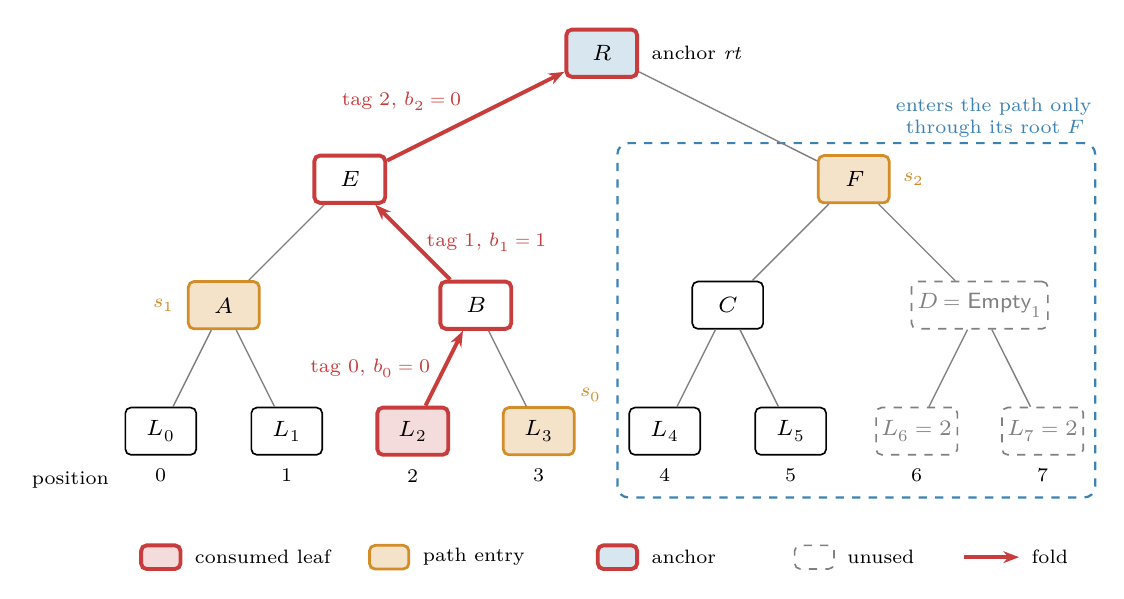
\begin{tikzpicture}[
  font=\footnotesize, >={Stealth[length=2mm]},
  nd/.style={draw=black, line width=0.6pt, rounded corners=2pt,
    inner sep=2pt, minimum height=6mm, minimum width=9mm},
  lf/.style={nd, draw=tierspend, line width=1.4pt, fill=tierspend,
    fill opacity=0.18, text opacity=1},
  rn/.style={nd, draw=tierspend, line width=1.4pt},
  sib/.style={nd, draw=tierfull, line width=1pt, fill=tierfull,
    fill opacity=0.25, text opacity=1},
  anc/.style={nd, draw=tierspend, line width=1.4pt, fill=tierin,
    fill opacity=0.2, text opacity=1},
  emp/.style={nd, draw=gray, dashed, text=gray},
  ed/.style={line width=0.5pt, gray},
  fold/.style={->, line width=1.4pt, tierspend},
  lb/.style={font=\scriptsize, inner sep=1.5pt, align=center},
]
\node[nd] (L0) at (0,0) {$L_0$};
\node[nd] (L1) at (1.6,0) {$L_1$};
\node[lf] (L2) at (3.2,0) {$L_2$};
\node[sib] (L3) at (4.8,0) {$L_3$};
\node[nd] (L4) at (6.4,0) {$L_4$};
\node[nd] (L5) at (8.0,0) {$L_5$};
\node[emp] (L6) at (9.6,0) {$L_6 = 2$};
\node[emp] (L7) at (11.2,0) {$L_7 = 2$};
\foreach \i in {0,...,7} {
  \node[lb, anchor=north] (P\i) at ([yshift=-1mm]L\i.south) {$\i$};
}
\node[lb, anchor=east] at (-0.6,-0.62) {position};
\node[sib] (A) at (0.8,1.6) {$A$};
\node[rn] (B) at (4.0,1.6) {$B$};
\node[nd] (C) at (7.2,1.6) {$C$};
\node[emp] (D) at (10.4,1.6) {$D = \mathsf{Empty}_1$};
\node[rn] (E) at (2.4,3.2) {$E$};
\node[sib] (F) at (8.8,3.2) {$F$};
\node[anc] (R) at (5.6,4.8) {$R$};
\node[lb, anchor=west] at ([xshift=1mm]R.east) {anchor $\mathit{rt}$};
\draw[ed] (L0) -- (A);
\draw[ed] (L1) -- (A);
\draw[ed] (L3) -- (B);
\draw[ed] (L4) -- (C);
\draw[ed] (L5) -- (C);
\draw[ed] (L6) -- (D);
\draw[ed] (L7) -- (D);
\draw[ed] (A) -- (E);
\draw[ed] (C) -- (F);
\draw[ed] (D) -- (F);
\draw[ed] (F) -- (R);
\draw[fold] (L2) -- node[lb, anchor=east, xshift=-1mm]
  {tag $0$, $b_0 = 0$} (B);
\draw[fold] (B) -- node[lb, anchor=west, xshift=1mm]
  {tag $1$, $b_1 = 1$} (E);
\draw[fold] (E) -- node[lb, anchor=south east, xshift=-1mm]
  {tag $2$, $b_2 = 0$} (R);
\node[lb, anchor=south west, text=tierfull] at (L3.north east) {$s_0$};
\node[lb, anchor=east, text=tierfull] at ([xshift=-1mm]A.west) {$s_1$};
\node[lb, anchor=west, text=tierfull] at ([xshift=1mm]F.east) {$s_2$};
\begin{scope}[on background layer]
\node[draw=tierin, dashed, line width=0.8pt, rounded corners=4pt,
  inner sep=4pt, fit=(F) (C) (D) (L4) (L7) (P4) (P7)] (box) {};
\end{scope}
\node[lb, anchor=south east, text=tierin] at (box.north east)
  {enters the path only\\through its root $F$};
\foreach \s/\t/\x in {lf/consumed leaf/0.0, sib/path entry/2.9,
    anc/anchor/5.8, emp/unused/8.3} {
  \node[\s, minimum width=5mm, minimum height=3mm, inner sep=0pt]
    (lg) at (\x,-1.6) {};
  \node[lb, anchor=west] at ([xshift=1mm]lg.east) {\t};
}
\draw[fold] (10.2,-1.6) -- (10.9,-1.6);
\node[lb, anchor=west] at (11.0,-1.6) {fold};
\end{tikzpicture}
\caption{A depth-$3$ instance of the note commitment tree of
\S\ref{sec:tree-hash}; the protocol's tree has depth $32$. Leaves $L_0$ to
$L_5$ are appended ($n = 6$); positions $6$ and $7$ hold
$\mathsf{Uncommitted}^{\mathsf{Orchard}} = 2$, so $D = \mathsf{Empty}_1$.
The consumed note's leaf is $L_2$, at position $2$ with bits $b_0 = 0$,
$b_1 = 1$, $b_2 = 0$. Its authentication path is $(s_0, s_1, s_2) =
(L_3, A, F)$, each entry the sibling of the route node at its level. The
bold fold $L_2 \to B \to E \to R$ evaluates $\mathsf{MerkleCRH}$ at each
level with the prefix $\mathrm{LE}_{10}(t)$, shown as tag $t$, and the
running value on the side given by $b_t$; it ends at the root $R$, the
anchor. By Lemma~\ref{lem:paths}, the entry $A$, left of the route, is the
root of a complete subtree and the same at every later anchor; the entry
$F$, right of the route and the root over positions $4$ to $7$, is a
function of the leaves appended at the anchor, with $2$ at unused positions,
and changes when $L_6$ or $L_7$ is appended; the entry $L_3$, right of the
route but already appended, is fixed at every later anchor. The boxed
subtree enters the path only through its root $F$. Every entry is computed
from $\mathsf{pos}$ and the first $n$ leaves.}
\label{fig:merklepath}
\end{figure}

Figure~\ref{fig:merklepath} shows the construction and
Lemma~\ref{lem:paths} on a tree of depth $3$.

\begin{remark}[Scope of hiding]
The anchor is public. The position, the consumed note's $\cmx$ and its
authentication path are not fields of the bundle, and the holder of the note
computes the path locally (Lemma~\ref{lem:paths}): obtaining the path of a
particular position from another party would disclose $\mathsf{pos}$ to that
party. The candidate set for the consumed note is the candidate set of the
anchor (\S\ref{sec:tree-anchors}), the positions of the $n$ appended leaves
of the anchored tree. Leaves that an observer knows by other means to be
commitments of dummy created notes (\S\ref{sec:notes-action}) or of notes
already consumed, and other data of the transaction, reduce the effective
set, so $n$ alone does not measure it. What an Action reveals is stated in
Theorem~\ref{thm:privacy} (``Privacy'', \S\ref{sec:security-privacy}).
\end{remark}

\section{Nullifiers}\label{sec:nf}

This section constructs the nullifier of a note, the nullifier sets that
consensus maintains per pool, and the rule that makes the nullifier of each
consumed note the element $\rho$ of the note created in the same Action. It
proves two properties of the construction: uniqueness, from discrete
logarithms on Pallas with $\GroupHash$ modelled as a random oracle; and, for
keys generated with $\mathsf{use\_qsk} = \mathsf{false}$, unlinkability, from
these two assumptions, the pseudorandomness of Poseidon and of PRF expansion,
and the joint hiding of the viewing keys. It also states what each key tier
can compute from nullifiers.

\subsection{The nullifier}\label{sec:nf-nullifier}

Requirement R3 of ``Requirements on a shielded payment''
(\S\ref{sec:intro-req}) excludes a second consumption of a note without a
public list of consumed notes. Each note therefore determines a
\emph{nullifier}, a tag published when the note is consumed, and a verifier
(\S\ref{sec:intro-structure}) rejects a nullifier already in the nullifier
set of its pool (\S\ref{sec:nf-sets}). The construction must make the nullifier
\begin{enumerate}
\item[(a)] \emph{deterministic}: a function of the note and of the nullifier
  deriving key $\nksym$ of the key that owns it, so that a second
  consumption publishes the same value; and
\item[(b)] \emph{unlinkable}: to a party without $\nksym$, the published
  value reveals nothing about the note's commitment or address.
\end{enumerate}

\begin{construction}[Nullifier PRF]
Let $f \colon \F_{p_{\Pallas}}^{3} \to \F_{p_{\Pallas}}^{3}$ be the Poseidon
permutation of width $t = 3$ over the Pallas base field, used as a sponge of
rate $2$ and capacity $1$, with S-box $x \mapsto x^{5}$, $8$ full and $56$
partial rounds (\emph{Crypto Guide}, \S``Arithmetisation-friendly hashing:
Poseidon'', Constructions ``The sponge construction'' and ``The Poseidon
permutation'', Example ``The Orchard Poseidon instance''). Its round
constants and MDS matrix are those of the protocol specification,
\S``$\mathsf{PoseidonHash}$ Function'', and are not reproduced. In
constant-input-length mode the hash
$\mathsf{PoseidonHash} \colon \F_{p_{\Pallas}} \times \F_{p_{\Pallas}} \to
\F_{p_{\Pallas}}$ is
\[
  \mathsf{PoseidonHash}(x, y) := \pi_1\bigl(f(x, y, 2^{65})\bigr),
\]
where $\pi_1$ is the projection onto the first component; the capacity
element $2^{65}$ encodes the input length $2$, so no padding is needed (same
citations). The \emph{nullifier PRF} is
\[
  \mathsf{PRF}^{\mathsf{nfOrchard}} \colon \F_{p_{\Pallas}} \times
    \F_{p_{\Pallas}} \to \F_{p_{\Pallas}}, \qquad
  \mathsf{PRF}^{\mathsf{nfOrchard}}_{\nksym}(\rho) :=
    \mathsf{PoseidonHash}(\nksym, \rho),
\]
keyed by the nullifier deriving key $\nksym \in \F_{p_{\Pallas}}$ of ``The
spending key and the spend-side secrets'' (\S\ref{sec:keys-sk}; protocol
specification,
\href{https://zips.z.cash/protocol/protocol.pdf#concreteprfs}%
{\S``Pseudo Random Functions''}).
\end{construction}

\begin{assumption}[Poseidon is a PRF]\label{ass:poseidon-prf}
For $\nksym$ uniform on $\F_{p_{\Pallas}}$, no efficient adversary with
adaptive oracle access distinguishes
$\rho \mapsto \mathsf{PoseidonHash}(\nksym, \rho)$ from a uniformly random
function $\F_{p_{\Pallas}} \to \F_{p_{\Pallas}}$, except with negligible
advantage: this is the game of Definition ``Pseudorandom function''
(\S\ref{sec:prim-prf}; \emph{Crypto Guide}, \S``Pseudorandom functions and
permutations'') with key, input and output sets $\F_{p_{\Pallas}}$. It is the
security requirement that the protocol specification,
\href{https://zips.z.cash/protocol/protocol.pdf#concreteprfs}%
{\S``Pseudo Random Functions''}, places on $\mathsf{PoseidonHash}$ keyed by
its first argument.
Its status is cryptanalytic: it is supported by the analysis of the Poseidon
round function (protocol specification, \S``$\mathsf{PoseidonHash}$
Function'', notes) and has no reduction to a standard problem
(\emph{Crypto Guide}, Example ``The Orchard Poseidon instance''). Of the
results of this section only Proposition~\ref{prop:nf-unlinkable} uses it;
Proposition~\ref{prop:nf-unique} uses no property of $\mathsf{PoseidonHash}$,
and the volume proves no unlinkability result for nullifiers without this
assumption.
\end{assumption}

\begin{definition}[Nullifier]\label{def:nullifier}
Let $K^{\mathsf{Orchard}} := \GroupHash(\texttt{z.cash:Orchard},
\texttt{K})$, the nullifier base, a fixed generator of
Table~\ref{tab:prim-grouphash}. For $\nksym, \rho, \psi \in \F_{p_{\Pallas}}$
and a point $\cmsym \in \Ep(\F_{p_{\Pallas}})$,
\[
  \mathsf{DeriveNullifier}_{\nksym}(\rho, \psi, \cmsym) :=
    \Extract_{\PP}\bigl([s]\,K^{\mathsf{Orchard}} + \cmsym\bigr)
    \in \F_{p_{\Pallas}},
\]
where
\[
  s := \bigl(\mathsf{PRF}^{\mathsf{nfOrchard}}_{\nksym}(\rho) + \psi\bigr)
    \bmod p_{\Pallas} \in \{0, \dots, p_{\Pallas} - 1\}:
\]
the sum of the two field elements is taken as its representative in
$\{0, \dots, p_{\Pallas} - 1\}$, and that integer multiplies
$K^{\mathsf{Orchard}}$. The \emph{nullifier} of a note
$n = (\mathsf{addr}, v, \rho, \psi, \rcm)$ whose note commitment $\cmsym$
(Definition~\ref{def:notecommit}) is not $\bot$, under the nullifier
deriving key $\nksym$ of the key that owns $\mathsf{addr}$, is
\[
  \nfsym := \mathsf{DeriveNullifier}_{\nksym}(\rho, \psi, \cmsym)
\]
(protocol specification, \S``Computing $\rho$ values and Nullifiers'').
\end{definition}

% compute/fields.py:
% [sec:prim-fields] bit length of p_Pallas = 255, of p_Vesta = 255;
%   p_Pallas < p_Vesta
\begin{remark}[Reduction modulo $p_{\Pallas}$]
The protocol specification attaches two notes to the definition
(\S``Computing $\rho$ values and Nullifiers''). First, the sum is reduced
modulo $p_{\Pallas}$ intentionally, although the scalar field of the Pallas
group is $\F_{p_{\Vesta}}$. Since $p_{\Pallas} < p_{\Vesta}$
(\S\ref{sec:prim-fields}), the representative in
$\{0, \dots, p_{\Pallas} - 1\}$ is a scalar without further reduction, by the
injective reading $\F_{p_{\Pallas}} \to \F_{p_{\Vesta}}$ of
\S\ref{sec:prim-fields}, and the multiplier of $K^{\mathsf{Orchard}}$ ranges
over $p_{\Pallas}$ of the $p_{\Vesta}$ scalars. Second, the inputs $\rho$ and
$\psi$ must be those of the note committed to by $\cmsym$.
\end{remark}

\begin{remark}[Determinism and masking]
For a fixed $\nksym$ the nullifier is a function of the fields $\rho$ and
$\psi$ of the note and of its commitment $\cmsym$, so a note has exactly one
nullifier under the $\nksym$ of its owner. That every accepted consumption of
the note publishes this value is Lemma~\ref{lem:one-nf}, proved in
``Double-spend resistance'' (\S\ref{sec:security-double-spend}) from the
Action statement, defined in ``The Action statement''
(\S\ref{sec:action-statement}). The point $[s]\,K^{\mathsf{Orchard}}$ is
added to $\cmsym$ before extraction. For notes of one key with pairwise
distinct $\rho$, the key generated with $\mathsf{use\_qsk} = \mathsf{false}$,
the multipliers are jointly pseudorandom to an efficient party that holds the
incoming viewing key and $\aksym^{\PP}$ but not $\nksym$, so the extracted
values give it no usable information on the commitments or on the address;
Proposition~\ref{prop:nf-unlinkable} states this exactly, under
Assumption~\ref{ass:poseidon-prf} and the further assumptions it names. The
element $\rho$ enters as the input of the PRF and $\psi$ as an additive term
of the multiplier. Both are fixed when the note is created: $\rho$ by
``Nullifier chaining'' (\S\ref{sec:nf-chaining}), and $\psi$ by the
derivation of \S\ref{sec:notes-seed}.
\end{remark}

\subsection{Nullifier sets}\label{sec:nf-sets}

Each verifier maintains, for each shielded pool, a \emph{nullifier set},
part of that pool's treestate (``Anchors'', \S\ref{sec:tree-anchors}). Every
Action publishes one nullifier, that of its consumed note, real or dummy
(\S\ref{sec:notes-action}), and the nullifiers published by the Actions of
valid transactions are inserted into the nullifier set of their pool
(protocol specification, \S``Nullifiers'' and \S``Nullifier Sets''). The
consensus rule of \S``Nullifier Sets'' is that a nullifier must not repeat,
either within a transaction or across transactions in a valid block chain;
a nullifier is compared only with nullifiers of its own pool, so equal values
in two pools do not repeat a nullifier (the specification treats the pools'
nullifiers as disjoint).

Both pools use the one derivation of Definition~\ref{def:nullifier}, with
the same PRF and the same nullifier base: the nullifier construction belongs
to the Orchard protocol, not to a pool (ZIP 229, Terminology). The Orchard
pool and the Ironwood pool keep separate nullifier sets, as they keep
separate note commitment trees, anchors and value pool balances (ZIP 229,
Rationale, ``Separate state''; protocol specification, \S``Nullifier
Sets''). The nullifier of an Ironwood-pool Action is inserted into, and
checked against, the nullifier set of the Ironwood pool only.

\begin{remark}[Pool locality]
Equal nullifier values in the two pools do not violate the consensus rule,
so every uniqueness property derived from it holds within one pool. In
particular the uniqueness of the elements $\rho$ proved in ``Double-spend
resistance'' (Corollary~\ref{cor:faerie-gold}) is uniqueness within a pool,
not across the two pools.
\end{remark}

\subsection{Nullifier chaining}\label{sec:nf-chaining}

\begin{construction}[Chaining rule]
In every Action the sender sets the element $\rho$ of the created note to the
nullifier that the same Action publishes for its consumed note,
\[
  \rho^{\mathsf{new}} := \nfsym^{\mathsf{old}} \in \F_{p_{\Pallas}},
\]
and encodes it as the $32$-byte string
$\mathsf{I2LEOSP}_{256}(\rho^{\mathsf{new}})$. When the Action consumes no
real note, its consumed side is a dummy note (Definition ``Dummy notes'',
\S\ref{sec:notes-action}), and the nullifier of that dummy note is
$\rho^{\mathsf{new}}$ (protocol specification, \S``Sending Notes
(Orchard)'', \S``Dummy Notes (Orchard)'' and \S``Faerie Gold attack and
fix'').
\end{construction}

Every Action has a consumed side (Definition ``Action'',
\S\ref{sec:notes-action}), so every note that an Action creates is
constructed with $\rho$ equal to the nullifier of that Action's consumed
note. The leaves that enter a pool's note commitment tree are the extracted
commitments of notes created by that pool's Actions (``The Merkle hash and
the tree'', \S\ref{sec:tree-hash}), so the rule covers every note whose
extracted commitment enters the tree. The consumed dummy note is not
created by an Action: its $\rho$ is $\Extract_{\PP}$ of a uniformly random
point of the Pallas group (\S\ref{sec:notes-action}).

The derivations of \S\ref{sec:notes-seed} take the chained $\rho$ as input:
with $\underline{\rho} := \mathsf{I2LEOSP}_{256}(\rho)$,
\begin{align*}
  \mathsf{esk} &= \mathrm{ToScalar}\bigl(\mathsf{PRFexpand}_{\mathsf{rseed}}
    ([\mathtt{0x04}] \,\|\, \underline{\rho})\bigr), &
  \psi &= \mathrm{ToBase}\bigl(\mathsf{PRFexpand}_{\mathsf{rseed}}
    ([\mathtt{0x09}] \,\|\, \underline{\rho})\bigr),
\end{align*}
and $\rcm$ is derived from the string $\mathsf{pre\_rcm}$, which contains
$\underline{\rho}$ and the encoding of $\psi$. Hence $\mathsf{esk}$ and $\psi$
are functions of $\mathsf{rseed}$ and of the nullifier that the note's own
Action publishes, and $\rcm$ is a function of these and of the remaining
note fields.

A \emph{Faerie Gold attack} is one in which a sender creates several notes to
one recipient that share a nullifier, so that only one of them can be spent
(protocol specification, \S``Faerie Gold attack and fix''). What a verifier
can rely on, the uniqueness of the elements $\rho$ within a pool and
resistance to the Faerie Gold attack, is proved in ``Double-spend
resistance'' (Corollary~\ref{cor:faerie-gold}) from the nullifier-set rule
and the Action statement, defined in ``The Action statement''
(\S\ref{sec:action-statement}). This subsection states the rule that an
honest sender follows and draws no conclusion about accepted notes from it.

\subsection{Nullifier uniqueness and unlinkability}\label{sec:nf-props}

% compute/fields.py:
% [sec:prim-sinsemilla] c = 253: 2^253 <= (p_Vesta - 1)/2 < 2^254
% compute/encodings.py:
% [sec:prim-sinsemilla] NoteCommit (g_d* || pk_d* || LE_64(v) || LE_255(rho)
%   || LE_255(psi)): 1086 bits, 109 chunks of 10 bits (padding 4); <= c = 253
\begin{proposition}[Nullifier uniqueness]\label{prop:nf-unique}
Under Assumptions~\ref{ass:dl-pallas} and~\ref{ass:grouphash-ro}, no
efficient adversary outputs, except with negligible probability, two notes
$n = (\mathsf{addr}, v, \rho, \psi, \rcm)$ and
$n' = (\mathsf{addr}', v', \rho', \psi', \rcm')$ and two nullifier deriving
keys $\nksym, \nksym' \in \F_{p_{\Pallas}}$, all of its choice, whose note
commitments $\cmsym$ and $\cmsym'$ are not $\bot$ and satisfy
$\cmsym \neq \cmsym'$ and
\[
  \mathsf{DeriveNullifier}_{\nksym}(\rho, \psi, \cmsym) =
  \mathsf{DeriveNullifier}_{\nksym'}(\rho', \psi', \cmsym').
\]
The adversary may hold every nullifier deriving key, and $\nksym = \nksym'$
and $\rho = \rho'$ are admitted. Since two distinct notes have distinct
commitments except with negligible probability
(Proposition~\ref{prop:cm}(b)), the same holds for two distinct notes in
place of two distinct commitments.
\end{proposition}

\begin{proof}
The adversary supplies both openings, so no knowledge extraction is used.
Let its output satisfy the conditions, and write
\begin{align*}
  K &:= K^{\mathsf{Orchard}}, \\
  Q &:= Q(\texttt{z.cash:Orchard-NoteCommit-M}), \\
  H_D &:= \GroupHash(\texttt{z.cash:Orchard-NoteCommit-r}, \varepsilon)
\end{align*}
for the nullifier base and for the hash base and the blinding base of
$\NoteCommit$ (Definition~\ref{def:notecommit}). A reduction that runs the
adversary computes $s := (\mathsf{PRF}^{\mathsf{nfOrchard}}_{\nksym}(\rho) +
\psi) \bmod p_{\Pallas}$ and $s'$ likewise; the pieces
$m = (m_1, \dots, m_{109})$ and $m'$ of the messages $M(n)$ and $M(n')$,
which have $109$ chunks of $k = 10$ bits (Table~\ref{tab:prim-sinsemilla});
and $\rcm$, $\rcm'$. Every coefficient below is therefore known to it, the
PRF outputs included, and no property of $\mathsf{PoseidonHash}$ is used.

Equal nullifiers are equal extracted coordinates, so by
Lemma~\ref{lem:opposite-points}
\[
  [s]\,K + \cmsym = \theta\bigl([s']\,K + \cmsym'\bigr)
  \qquad \text{for some } \theta \in \{1, -1\}.
\]
Since $\cmsym \neq \bot$, its hash point is not $\bot$, and by the unrolled
form~\eqref{eq:prim-unfold} of the proof of
Proposition~\ref{prop:sinsemilla-cr},
\[
  \cmsym = [2^{109}]\,Q + \sum_{j=0}^{2^{k}-1} [\chi_j(m)]\,S(j)
    + [\rcm]\,H_D, \qquad
  \chi_j(m) = \sum_{i=1}^{109} 2^{109-i}\,\delta_{m_i, j},
\]
and likewise for $\cmsym'$. Substituting gives, with coefficients in
$\F_{p_{\Vesta}}$ and $s$, $s'$ read as scalars,
\begin{equation}\label{eq:nf-relation}
  [s - \theta s']\,K + [(1 - \theta)\, 2^{109}]\,Q
  + \sum_{j} [\chi_j(m) - \theta\, \chi_j(m')]\,S(j)
  + [\rcm - \theta\, \rcm']\,H_D = \mathcal{O}.
\end{equation}
The relation is non-trivial in each case.
\begin{itemize}
\item If $\theta = -1$, the coefficient of $Q$ is $2^{110}$, non-zero
  modulo $p_{\Vesta}$ because $0 < 2^{110} < 2^{253} \le (p_{\Vesta} - 1)/2$.
\item If $\theta = 1$ and $M(n) \neq M(n')$, then $m \neq m'$, and
  $\chi(m) \neq \chi(m')$ modulo $p_{\Vesta}$ by step~(1) of the proof of
  Proposition~\ref{prop:sinsemilla-cr} ($109 \le c = 253$); some coefficient
  of an $S(j)$ is non-zero.
\item If $\theta = 1$ and $M(n) = M(n')$, then $\rcm \neq \rcm'$, since
  equal messages and equal trapdoors give $\cmsym = \cmsym'$; the coefficient
  of $H_D$ is non-zero.
\end{itemize}
The points $K$, $Q$, $S(0), \dots, S(2^{k} - 1)$ and $H_D$ are values of
$\GroupHash$ on pairwise distinct inputs (Table~\ref{tab:prim-grouphash}).
The reduction outputs these inputs with the coefficients
of~\eqref{eq:nf-relation}, a non-trivial relation with known coefficients.
By the lemma on relations among fixed generators
(\S\ref{sec:prim-sinsemilla}), the reduction behind
Proposition~\ref{prop:sinsemilla-cr}, this happens with negligible
probability under Assumptions~\ref{ass:dl-pallas}
and~\ref{ass:grouphash-ro}. The specification records that its Sinsemilla
collision argument extends to additional terms with independent bases for
this purpose (protocol specification, \S``Sinsemilla Hash Function'',
Security argument, note; \S``Faerie Gold attack and fix'').

For distinct notes whose commitments are not $\bot$, equal commitments have
negligible probability by Proposition~\ref{prop:cm}(b), and distinct
commitments are the case above.
\end{proof}

\begin{remark}[Scope of Proposition~\ref{prop:nf-unique}]
The proposition uses no pseudorandomness of $\mathsf{PoseidonHash}$, and
none could be used: the adversary holds the PRF keys, and the reduction
knows every coefficient. It does not require distinct elements $\rho$, which
the specification's security requirement assumes
(\href{https://zips.z.cash/protocol/protocol.pdf#rhoandnullifiers}%
{\S``Computing $\rho$ values and Nullifiers''}). Two notes with equal
commitments are equal except
with negligible probability (Proposition~\ref{prop:cm}(b)) and so have equal
nullifiers under one $\nksym$. Excluding equal commitments among the notes of
a pool is the role of the chaining rule of \S\ref{sec:nf-chaining}, as
Corollary~\ref{cor:faerie-gold} proves.
\end{remark}

% compute/fields.py:
% [sec:nf-props] uniform residue mod p_Pallas read as a scalar vs uniform
%   scalar mod p_Vesta: distance (p_Vesta - p_Pallas)/p_Vesta
%   = 2^-167.84 < 2^-167
% [sec:prim-prf] ToBase (mod p_Pallas): Math Guide bound m/2^512
%   = 2^-258 (1 + e), 0 < e < 2^-128, so < 2^-257
% [sec:prim-prf] ToScalar (mod p_Vesta): Math Guide bound m/2^512
%   = 2^-258 (1 + e), 0 < e < 2^-128, so < 2^-257
\begin{proposition}[Nullifier unlinkability]\label{prop:nf-unlinkable}
Let a key be generated with $\mathsf{use\_qsk} = \mathsf{false}$ from a
uniform spending key, as in \S\ref{sec:keys-sk} and \S\ref{sec:keys-viewing},
with nullifier deriving key $\nksym$. An adversary receives the incoming
viewing key $(\dk, \ivk)$ and the point $\aksym^{\PP}$ of the key, but not
$\nksym$. It then submits, adaptively, notes
$n_i = (\mathsf{addr}_i, v_i, \rho_i, \psi_i, \rcm_i)$, $1 \le i \le q$, of
its choice, with pairwise distinct $\rho_i$ and note commitments
$\cmsym_i \neq \bot$, and after each submission receives an answer:
\begin{itemize}
\item in the \emph{real game},
  $\nfsym_i := \mathsf{DeriveNullifier}_{\nksym}(\rho_i, \psi_i, \cmsym_i)$;
\item in the \emph{ideal game},
  $\Extract_{\PP}([u_i]\,K^{\mathsf{Orchard}} + \cmsym_i)$ for $u_i$ uniform
  on $\F_{p_{\Vesta}}$, independent of each other and of all else.
\end{itemize}
It outputs a bit. Let $\delta := (p_{\Vesta} - p_{\Pallas})/p_{\Vesta}$,
which is below $2^{-167}$, the statistical distance between the uniform
distribution on $\{0, \dots, p_{\Pallas} - 1\}$, read in $\F_{p_{\Vesta}}$,
and the uniform distribution on $\F_{p_{\Vesta}}$. Then the difference of the
probabilities that it outputs $1$ in the two games is at most
\[
  2\bigl(\epsilon_{\mathsf{key}} + \epsilon_{\mathsf{expand}}
    + 3 \cdot 2^{-257} + \epsilon_{\mathsf{vk}}\bigr)
  + \epsilon_{\mathsf{Pos}} + q\,\delta,
\]
where $\epsilon_{\mathsf{expand}}$, $\epsilon_{\mathsf{vk}}$ and
$\epsilon_{\mathsf{Pos}}$ are the largest advantages against
Assumptions~\ref{ass:prf-expand} (through
Lemma~\ref{lem:prf-independence}), \ref{ass:vk-hiding}
and~\ref{ass:poseidon-prf} of the algorithms built from the adversary in the
proof, and $\epsilon_{\mathsf{key}}$ is the probability that a single draw of
key generation from a uniform spending key is rejected plus the probability
that $\ask = 0$ or $\hat{M} = \bot$ for independent uniform $(\ask, \nksym)$,
with $\hat{M}$ the hash point of $\CommitIvk$ on $(\aksym, \nksym)$
(\S\ref{sec:keys-viewing}). The
term $\epsilon_{\mathsf{key}}$ is negligible under
Assumptions~\ref{ass:prf-expand}, \ref{ass:dl-pallas}
and~\ref{ass:grouphash-ro} (Lemma ``Rejection in key generation'',
\S\ref{sec:keys-viewing}); the bound is therefore negligible for every
efficient adversary, whose number $q$ of queries is polynomial, under these
assumptions and Assumptions~\ref{ass:vk-hiding} and~\ref{ass:poseidon-prf}.
When $K^{\mathsf{Orchard}} \neq \mathcal{O}$, the point
$[u_i]\,K^{\mathsf{Orchard}} + \cmsym_i$ is uniform on $\Ep(\F_{p_{\Pallas}})$
whatever $\cmsym_i$ is, so the ideal answers are independent of the notes
and of each other; in the model of
Assumption~\ref{ass:grouphash-ro}, $K^{\mathsf{Orchard}} = \mathcal{O}$ has
probability $1/p_{\Vesta}$.
\end{proposition}

\begin{proof}
Write $K := K^{\mathsf{Orchard}}$. The proof passes from the real game $H_0$
through hybrid games $H_1, \dots, H_5$; each hop changes the probability of
the output $1$ by at most the amount stated (\emph{Crypto Guide},
\S``The hybrid argument'', Lemma ``Hybrid lemma''), and each reduction runs
the adversary and the rest of the game.

\emph{Hybrid $H_1$: idealised key.} The key is generated by a single draw from a
uniform $\mathsf{sk}$, without rejection, at the cost of the probability that
the draw is rejected (Lemma ``Rejection in key generation'',
\S\ref{sec:keys-viewing}). Then $(\ask, \nksym, \rivk)$ is replaced by
independent uniform elements of $\F_{p_{\Vesta}}$, $\F_{p_{\Pallas}}$ and
$\F_{p_{\Vesta}}$, from which the
other components are derived as in \S\ref{sec:keys-sk}
and~\S\ref{sec:keys-viewing}. By Lemma~\ref{lem:prf-independence}, this costs at
most $\epsilon_{\mathsf{expand}}$ plus the three reduction distances, each below
$2^{-257}$ (\S\ref{sec:prim-prf}): the three inputs of
$\mathsf{PRFexpand}_{\mathsf{sk}}$ have distinct lead bytes, and the game is an
efficient function of the triple, which derives $\aksym^{\PP}$, $\ivk$ and
$\dk$, runs the adversary and answers each query with the nullifier under
$\nksym$.

\emph{Hybrid $H_2$: joint hiding.} When $\ask \neq 0$, the pair $(\ivk, \dk)$ is
replaced by $(\CommitIvk_{\rivk'}(\aksym, \nksym), u)$, for $\rivk'$ uniform on
$\F_{p_{\Vesta}}$ and $u$ a uniform $32$-byte string, independent of all else.
The cost is at most $\epsilon_{\mathsf{vk}}$. The reduction for
Assumption~\ref{ass:vk-hiding} draws $\ask$ and $\nksym$ itself; for $\ask \neq
0$ the pair $(\aksym, \nksym)$ lies in the domain of the assumption
(\S\ref{sec:keys-sk}). It receives a triple for that pair, passes its first two
components to the adversary as $\ivk$ and $\dk$, together with $\aksym^{\PP}$,
and answers every query with the nullifier under its own $\nksym$. Giving
$\aksym^{\PP}$ costs nothing, because after $H_1$ the scalar $\ask$ is
independent of $(\nksym, \rivk)$ and the assumption holds for every fixed
$(\aksym, \nksym)$.

\emph{Hybrid $H_3$: independent viewing keys.} The pair $(\ivk, \dk)$ is
replaced, whatever $\ask$ is, by $(\Extract_{\PP}(W), u)$ for a uniform point
$W$ and a uniform $32$-byte string $u$, independent of all else. When
$\ask \neq 0$ and the hash point $\hat{M}$ of the message
$\mathrm{LE}_{255}(\aksym) \,\|\, \mathrm{LE}_{255}(\nksym)$ is not $\bot$,
the commitment point $\hat{M} + [\rivk']\,H_D$ is uniform on
$\Ep(\F_{p_{\Pallas}})$ by Lemma~\ref{lem:sinsemilla-commit}(i), its blinding
base $H_D$ not being $\mathcal{O}$ (\S\ref{sec:keys-viewing}), so the two
games are identically distributed conditioned on that event, which depends
on $(\ask, \nksym)$ only. The cost is at most the probability that
$\ask = 0$ or $\hat{M} = \bot$, the remaining part of
$\epsilon_{\mathsf{key}}$. In $H_3$
the key $\nksym$ enters the game only through the answers: $\dk$, $\ivk$ and
$\aksym^{\PP}$ are independent of it.

\emph{Hybrid $H_4$: random function.} The function
$\mathsf{PRF}^{\mathsf{nfOrchard}}_{\nksym}$ is replaced by a uniformly
random function $F \colon \F_{p_{\Pallas}} \to \F_{p_{\Pallas}}$. The cost is
at most $\epsilon_{\mathsf{Pos}}$: the reduction for
Assumption~\ref{ass:poseidon-prf} runs $H_3$ with its oracle in place of
$\mathsf{PRF}^{\mathsf{nfOrchard}}_{\nksym}$, since $\nksym$, uniform on
$\F_{p_{\Pallas}}$, is used nowhere else. In $H_4$ the $i$-th answer is
$\Extract_{\PP}([s_i]\,K + \cmsym_i)$ with
$s_i := (F(\rho_i) + \psi_i) \bmod p_{\Pallas}$. The $\rho_i$ are pairwise
distinct, so, with $F$ sampled lazily, $F(\rho_i)$ is uniform on
$\F_{p_{\Pallas}}$ and independent of everything the adversary has received
when it submits $n_i$. Translation by $\psi_i$ is a bijection modulo
$p_{\Pallas}$, so $s_i$ is uniform on $\{0, \dots, p_{\Pallas} - 1\}$ and
independent of that view, whatever $\psi_i$ is.

\emph{Hybrid $H_5$: uniform scalars.} For $i = 1, \dots, q$ in turn, the
scalar $s_i$, read in $\F_{p_{\Vesta}}$ (\S\ref{sec:prim-fields}), is replaced
by $u_i$ uniform on $\F_{p_{\Vesta}}$. The two distributions differ by
$1/p_{\Pallas} - 1/p_{\Vesta}$ on each of the $p_{\Pallas}$ residues and by
$1/p_{\Vesta}$ on each of the other $p_{\Vesta} - p_{\Pallas}$ scalars, so
their statistical distance is
\[
  \tfrac{1}{2}\Bigl(p_{\Pallas}\Bigl(\frac{1}{p_{\Pallas}}
    - \frac{1}{p_{\Vesta}}\Bigr)
    + \frac{p_{\Vesta} - p_{\Pallas}}{p_{\Vesta}}\Bigr)
  = \frac{p_{\Vesta} - p_{\Pallas}}{p_{\Vesta}} = \delta.
\]
The rest of the game is a randomised function of the view before the $i$-th
answer and of the replaced value, which is independent of that view; each
step therefore costs at most $\delta$, and the $q$ steps at most $q\,\delta$
(\emph{Math Guide}, \S``Statistical distance'', Theorem ``Properties of
statistical distance'', parts~(2) and~(4)).

In $H_5$ the answers are those of the ideal game, and the key material is
that of $H_3$. Neither in $H_5$ nor in the ideal game do the answers depend
on the key, so the hops of $H_3$, $H_2$ and $H_1$, taken in reverse order
with the answers of the ideal game, lead from $H_5$ to the ideal game at the
same costs. Summing the costs of both passes gives the bound. The last
statement of the proposition holds because, for $K \neq \mathcal{O}$, the
map $u \mapsto [u]\,K$ is a bijection from $\F_{p_{\Vesta}}$ onto the group
of prime order $p_{\Vesta}$, and translation by $\cmsym_i$ is a bijection of
the group; under Assumption~\ref{ass:grouphash-ro} the point $K$ is uniform.
\end{proof}

\begin{remark}[Design statement, not proved]
The specification describes the nullifier as combining elliptic-curve
cryptography with the Poseidon-based PRF so as to give privacy defence in
depth against a weakness in either (protocol specification, \S``Faerie Gold
attack and fix''). It states that, under the weaker assumption that
$\mathsf{PoseidonHash}$ preserves sufficient entropy from $\nksym$ and
$\rho$, the construction would remain unlinkable under a decisional
Diffie--Hellman assumption on Pallas even if the Poseidon-based PRF were
distinguishable from an ideal PRF (\S``$\mathsf{PoseidonHash}$ Function'',
note; \emph{Crypto Guide}, \S``Diffie--Hellman: computational and
decisional'', Definition ``Decisional Diffie--Hellman, DDH''; the form
assumed in this volume is Assumption~\ref{ass:ddh-pallas}). The volume
records this as the specification's design statement and derives no result
from it; Proposition~\ref{prop:nf-unlinkable} relies on
Assumption~\ref{ass:poseidon-prf} instead.
\end{remark}

For keys with $\mathsf{use\_qsk} = \mathsf{false}$, the key tiers of
Proposition~\ref{prop:capabilities} (``Capability separation'') have the
following powers over nullifiers. The full viewing key
$(\aksym, \nksym, \rivk)$ contains $\nksym$. Its holder computes
$\mathsf{DeriveNullifier}_{\nksym}(\rho, \psi, \cmsym)$ for every note of the
key whose fields it knows, and tests whether that value is in the nullifier
set of the note's pool; that every accepted consumption of the note
publishes this value is Lemma~\ref{lem:one-nf}. It does so without spending
authority, since the full viewing key yields no $\ask$
(Proposition~\ref{prop:capabilities}(a)). A holder of only the incoming
viewing key $(\dk, \ivk)$ cannot link a nullifier to its note, for notes with
pairwise distinct $\rho$, by Proposition~\ref{prop:nf-unlinkable}.

\begin{remark}[Limits]
Proposition~\ref{prop:nf-unlinkable} gives nothing against a holder of
$\nksym$, which includes every holder of the full viewing key: such a holder
recomputes, and so links, the nullifier of every note of the key whose
fields it knows. It does not concern links through other public data, such
as timing or the structure of the transaction; the privacy of an Action,
with its preconditions, is Theorem~\ref{thm:privacy}, in ``Privacy''
(\S\ref{sec:security-privacy}).
\end{remark}

\section{Spend authorisation}\label{sec:spendauth}

This section instantiates RedDSA, the re-randomisable Schnorr signature
scheme of the \emph{Crypto Guide}, on the Pallas group; constructs the
randomised validating key and the spend-authorisation signature of an Action;
and proves two properties of them: the published key is, with the signature
scheme's hash modelled as a random oracle, within negligible statistical
distance of a key independent of the spend validating key; and a new valid
signature under a randomised key yields the key's discrete logarithm. The
signed message is a parameter throughout; ``Transaction digests and
signatures'' (\S\ref{sec:tx-sighash}) fixes it.

\subsection{The RedPallas signature scheme}\label{sec:spendauth-redpallas}

\begin{remark}[Spending authority and its signature]
Requirement R5 of ``Requirements on a shielded payment''
(\S\ref{sec:intro-req}) admits only the holder of a note's spending authority
as a party that consumes the note. For keys generated with
$\mathsf{use\_qsk} = \mathsf{false}$, the spending authority over the notes of
every address derived from a spending key is knowledge of its spend
authorising key $\ask$ of ``The spending key and the spend-side secrets''
(\S\ref{sec:keys-sk}), the discrete logarithm of
$\aksym^{\PP} = [\ask]\,G^{\mathsf{SpendAuth}}$ to the base
$G^{\mathsf{SpendAuth}}$. No lower key tier yields $\ask$, since every lower
tier is computed from the full viewing key
(Proposition~\ref{prop:capabilities}(a)). Each Action therefore carries a
signature that only a holder of $\ask$ can produce, under a validating key
that does not link Actions consuming notes of the same key: a fresh
re-randomisation of $\aksym^{\PP}$ (\S\ref{sec:spendauth-rk}), never
$\aksym^{\PP}$ itself. Theorem~\ref{thm:spend-authority}, in ``Authorisation
of spends'' (\S\ref{sec:security-auth}), proves for keys with
$\mathsf{use\_qsk} = \mathsf{false}$ that no efficient party without $\ask$
produces an accepted Action that consumes a note of an honestly generated
address and whose spend-authorisation signature is on a digest that the key
holder did not sign under the Action's randomised key, except with negligible
probability.
\end{remark}

\begin{definition}[RedPallas hash]
The \emph{RedPallas hash} is the map $\mathsf{H}$ from byte strings to
$64$-byte strings
\[
  \mathsf{H}(z) := \mathrm{BLAKE2b\text{-}512}(\texttt{Zcash\_RedPallasH},
    z),
\]
with the notation of the expansion function (\S\ref{sec:prim-prf}) and the
$16$-byte personalisation $\texttt{Zcash\_RedPallasH}$. Its reduction to
scalars is
\[
  \mathsf{H}^{\circledast}(z) := \mathsf{LEOS2IP}_{512}\bigl(\mathsf{H}(z)\bigr)
    \bmod p_{\Vesta} = \mathrm{ToScalar}\bigl(\mathsf{H}(z)\bigr)
    \in \F_{p_{\Vesta}}
\]
(protocol specification, \S``RedDSA, RedJubjub, and RedPallas'' and
\S``BLAKE2 Hash Functions''). The symbol $\mathsf{H}^{\circledast}$ is that of
the specification and of the \emph{Crypto Guide}'s Remark ``RedDSA as
deployed'' (\S``RedDSA: re-randomisable Schnorr for Orchard''); it is
distinct from the star encoding $P^{\star}$ of a point.
\end{definition}

% compute/fields.py:
% [sec:prim-prf] GenRandom: H* output mod p_Vesta, H* a random oracle:
%   Math Guide bound m/2^512 = 2^-258 (1 + e), 0 < e < 2^-128, so < 2^-257;
%   exact distance t(m-t)/(m 2^512) = 2^-260.99
\begin{assumption}[The RedPallas hash as a random oracle]\label{ass:hstar-ro}
In security arguments the RedPallas hash $\mathsf{H}$ is modelled as a random
oracle with output length $512$, that is, with range the $64$-byte strings,
queried by every party (\emph{Crypto Guide}, \S``The random oracle model'',
Definition ``Random oracle''). Consequently $\mathsf{H}^{\circledast}$ is a
random function into $\F_{p_{\Vesta}}$: its values at distinct inputs are
independent, and each is distributed as $\mathrm{ToScalar}(U)$ for $U$
uniform on the $64$-byte strings. That distribution is at statistical
distance at most
\[
  \delta_{512} := p_{\Vesta} / 2^{512} < 2^{-257}
\]
from the uniform distribution on $\F_{p_{\Vesta}}$ (\emph{Math Guide},
\S``Uniform sampling and the bias of modular reduction'', Proposition ``Bias
of modular reduction'', with $L = 512$), and it gives each scalar probability
at most $1/p_{\Vesta} + 2^{-512}$, since each residue has at most
$\lfloor 2^{512}/p_{\Vesta} \rfloor + 1$ preimages among the $2^{512}$
strings. The assumption is a heuristic about BLAKE2b, not a theorem. Every
later result on RedPallas signatures or on the randomiser generator below
names it.
\end{assumption}

\begin{construction}[RedPallas]
RedPallas is the \emph{Crypto Guide}'s Construction ``RedDSA''
(\S``RedDSA: re-randomisable Schnorr for Orchard'') on the Pallas group
$\Ep(\F_{p_{\Pallas}})$, of prime order $p_{\Vesta}$, with both hashes
$\mathsf{H}^{\circledast}$ and with a base point $B \neq \mathcal{O}$ as
parameter; the group having prime order, $B$ generates it. For a point $P$
let $\underline{P} := \mathsf{LEBS2OSP}_{256}(P^{\star})$, its $32$-byte
encoding; the map $P \mapsto \underline{P}$ is injective, as the star
encoding is (\S\ref{sec:prim-fields}) and $\mathsf{LEBS2OSP}_{256}$ is a
bijection onto the $32$-byte strings. Messages are byte strings.
\begin{enumerate}
\item \emph{Keys.} A signing key is a scalar $x \in \F_{p_{\Vesta}}$; its
  validating key is $X := [x]\,B$.
\item \emph{Signing} a message $M$ under $x$: draw $T$ uniformly from the
  $80$-byte strings, where $80 = (512 + 128)/8$ is the specification's
  randomness length for a $512$-bit hash; let
  \begin{align*}
    r &:= \mathsf{H}^{\circledast}(T \,\|\, \underline{X} \,\|\, M), &
    R &:= [r]\,B, \\
    c &:= \mathsf{H}^{\circledast}(\underline{R} \,\|\, \underline{X}
      \,\|\, M), &
    S &:= r + c \cdot x \in \F_{p_{\Vesta}},
  \end{align*}
  and output the $64$-byte signature
  $\sigma := \underline{R} \,\|\, \mathsf{I2LEOSP}_{256}(S)$.
\item \emph{Validation} of a $64$-byte string $\sigma$ under a point $X$ on
  $M$: let $\bar{R}$ be the first $32$ bytes of $\sigma$ and $\bar{S}$ the
  last $32$; let
  $R := \mathsf{abst}_{\PP}(\mathsf{LEBS2OSP}_{256}^{-1}(\bar{R}))$,
  $S := \mathsf{LEOS2IP}_{256}(\bar{S})$ and
  $c := \mathsf{H}^{\circledast}(\bar{R} \,\|\, \underline{X} \,\|\, M)$.
  Accept if and only if $R \neq \bot$, $S < p_{\Vesta}$ and
  \begin{equation}\label{eq:spendauth-verify}
    [S]\,B = R + [c]\,X .
  \end{equation}
\end{enumerate}
(Protocol specification, \S``RedDSA, RedJubjub, and RedPallas''; its
validation equation carries the cofactor, which is $1$ on Pallas.)
\end{construction}

The partial inverse $\mathsf{abst}_{\PP}$ returns $\bot$ on every $256$-bit
string that is not the star encoding of a point (\S\ref{sec:prim-fields});
validation therefore rejects a non-canonical $\bar{R}$, and an accepted
signature has $\bar{R} = \underline{R}$. An honest signature is accepted: its
first half $\underline{R}$ decodes to $R$, its $S$ is an integer
representative below $p_{\Vesta}$, the verifier recomputes the signer's
$c$, and $[S]\,B = [r]\,B + [c \cdot x]\,B = R + [c]\,X$ (\emph{Crypto
Guide}, \S``From identification to signature via the Fiat--Shamir
transform'', Proposition ``Perfect correctness''). Both the nonce hash and the
challenge hash take the encoded validating key $\underline{X}$: the scheme is
\emph{key-prefixed}. The message $M$ is a parameter: the message of every
RedPallas signature in this volume is the signature digest constructed in
``Transaction digests and signatures'' (\S\ref{sec:tx-sighash}), and no
argument before that subsection depends on its value.

\begin{definition}[Spend-authorisation and binding-signature instances]
The volume uses two instances of RedPallas, which share the signing and
validation algorithms and differ in the base $B$ and in the use of key
re-randomisation (protocol specification,
\href{https://zips.z.cash/protocol/protocol.pdf#concretespendauthsig}%
{\S``Spend Authorization Signature (Sapling and Orchard)''} and
\S``Binding Signature (Sapling and Orchard)''):
\begin{enumerate}
\item the \emph{spend-authorisation instance}, with key re-randomisation
  (\S\ref{sec:spendauth-rk}) and base
  \[
    B = G^{\mathsf{SpendAuth}} = \GroupHash(\texttt{z.cash:Orchard},
    \texttt{G});
  \]
\item the \emph{binding-signature instance}, without re-randomisation, used
  in ``The binding signature'' (\S\ref{sec:value-bsig}), with base the
  value-commitment randomness base
  \[
    B = R^{\mathsf{Orchard}} = \GroupHash(\texttt{z.cash:Orchard-cv},
    \texttt{r}).
  \]
\end{enumerate}
Both bases are rows of Table~\ref{tab:prim-grouphash}
(\S\ref{sec:prim-grouphash}); the specification takes each as the generator
parameter of RedDSA.
\end{definition}

\begin{definition}[Randomiser generator and key re-randomisation]
The \emph{randomiser generator} $\mathsf{GenRandom}$ draws $T$ uniformly from
the $80$-byte strings and returns $\mathsf{H}^{\circledast}(T) \in
\F_{p_{\Vesta}}$ (protocol specification, \S``RedDSA, RedJubjub, and
RedPallas''); its distance from uniform is bounded in
\S\ref{sec:spendauth-rk}. \emph{Re-randomisation} by a randomiser
$\alpha \in \F_{p_{\Vesta}}$ maps a key pair $(x, X)$ to
$(x + \alpha,\, X + [\alpha]\,B)$ (\emph{Crypto Guide}, \S``Key
re-randomisation and unlinkability'', Definition ``Key re-randomisation'').
\end{definition}

\begin{remark}[Key prefixing]
Let $\sigma$ be valid under $X$ on $M$, with decoded components $R$ and $S$
and challenge
$c = \mathsf{H}^{\circledast}(\underline{R} \,\|\, \underline{X} \,\|\, M)$,
and let $X' := X + [\beta]\,B \neq \mathcal{O}$ for a scalar $\beta \neq 0$.
The shifted string
$\sigma' := \underline{R} \,\|\, \mathsf{I2LEOSP}_{256}(S + c\beta)$
satisfies $[S + c\beta]\,B = R + [c]\,X'$. Validation of $\sigma'$ under
$X'$, however, recomputes the challenge as
$c' := \mathsf{H}^{\circledast}(\underline{R} \,\|\, \underline{X'} \,\|\,
M)$, the value of the oracle at an input other than that of $c$, since
$\underline{X'} \neq \underline{X}$; and~\eqref{eq:spendauth-verify} holds
for $\sigma'$ under $X'$ only if $[c - c']\,X' = \mathcal{O}$, that is, only
if $c' = c$. Under Assumption~\ref{ass:hstar-ro}, for each $\beta$ the value
$c'$ is independent of $c$ and equals it with probability at most
$1/p_{\Vesta} + 2^{-512}$. A signature is therefore not transported from one
key to a related key by shifting its response. With a challenge that omitted
the key, $c' = c$ always, and the shift would turn every signature under $X$
into one under $X'$ (\emph{Crypto Guide}, \S``From identification to
signature via the Fiat--Shamir transform'', Remark ``Two conventions'';
\S``Key re-randomisation and unlinkability'', Remark ``Unforgeability under
re-randomised keys, and the key-prefixing subtlety''). The proof of
Proposition~\ref{prop:redpallas-euf}, which admits randomisers chosen by the
adversary, uses key prefixing in its steps~(3) and~(5).
\end{remark}

\FloatBarrier
\subsection{Randomised validating keys}\label{sec:spendauth-rk}

\begin{construction}[Randomised validating key]
For each Action the spender draws a \emph{spend-authorisation randomiser}
$\alpha := \mathsf{GenRandom}()$, independently of every other draw, and sets
\[
  \rsk := \ask + \alpha \in \F_{p_{\Vesta}}, \qquad
  \rk := \aksym^{\PP} + [\alpha]\,G^{\mathsf{SpendAuth}}
    \in \Ep(\F_{p_{\Pallas}}),
\]
with $\ask$ the sign-normalised spend authorising key of the spending key of
the consumed note and $\aksym^{\PP}$ its spend validating key
(\S\ref{sec:keys-sk}). Since $\aksym^{\PP} = [\ask]\,G^{\mathsf{SpendAuth}}$,
it follows that $\rk = [\rsk]\,G^{\mathsf{SpendAuth}}$ (\emph{Crypto Guide},
\S``Key re-randomisation and unlinkability'', Proposition
``Re-randomisation consistency''), so $(\rsk, \rk)$ is a key pair of the
spend-authorisation instance. The Action publishes the \emph{randomised
validating key} $\rk$ and its \emph{spend-authorisation signature}, the
RedPallas signature under $\rsk$ on the signature digest constructed in
``Transaction digests and signatures'' (\S\ref{sec:tx-sighash}); it
publishes none of $\ask$, $\alpha$, $\rsk$, $\aksym^{\PP}$ and $\aksym$
(protocol specification,
\href{https://zips.z.cash/protocol/protocol.pdf#spendauthsig}%
{\S``Spend Authorization Signature (Sapling and Orchard)''}).
\end{construction}

% compute/fields.py:
% [sec:prim-prf] GenRandom: H* output mod p_Vesta, H* a random oracle:
%   Math Guide bound m/2^512 = 2^-258 (1 + e), 0 < e < 2^-128, so < 2^-257
% [sec:spendauth-rk] GenRandom hashes 80 uniform bytes (640 bits) to a
%   512-bit H* output; the distance is that of the 512-bit reduction above,
%   not of a 640-bit one
\begin{lemma}[Distance of GenRandom from uniform]
Under Assumption~\ref{ass:hstar-ro}, let an algorithm, the observer, make at
most $q_h$ queries to $\mathsf{H}$ and, at one point, choose a byte string
$w$ and receive $\alpha := \mathsf{H}^{\circledast}(T \,\|\, w)$, for $T$
uniform on the $80$-byte strings and independent of all else. The pair
formed by the observer's view and $\alpha$ is within statistical distance
\begin{equation}\label{eq:spendauth-genrandom}
  \delta_{512} + q_h \cdot 2^{-640}
\end{equation}
of the pair obtained when $\alpha$ is replaced by a uniform element of
$\F_{p_{\Vesta}}$ independent of all else. A randomiser from
$\mathsf{GenRandom}$ is the case $w = \varepsilon$; the nonce of a RedPallas
signature under $X$ on $M$ is the case $w = \underline{X} \,\|\, M$. The first
term of~\eqref{eq:spendauth-genrandom} is set by the $512$-bit output of
$\mathsf{H}$, not by the $640$-bit length of $T$; the length of $T$ enters
only the second term.
\end{lemma}

\begin{proof}
Let $E$ be the event that the observer queries $\mathsf{H}$ at
$T \,\|\, w$. In a second experiment, $\mathsf{H}(T \,\|\, w)$ is replaced,
in the computation of $\alpha$ only, by a uniform $64$-byte string $U$
independent of all else. In the lazy realisation of the random oracle
(\emph{Crypto Guide}, \S``The random oracle model'', Definition ``Random
oracle'') the answers at inputs
other than $T \,\|\, w$ are independent of $\mathsf{H}(T \,\|\, w)$, so the
two experiments are identical until $E$ occurs; $E$ has the same probability
in both, and their outputs are within statistical distance $\Pr[E]$
(\emph{Crypto Guide}, \S``Security as a game'', Remark ``Game-hopping''). In
the second experiment the observer's view is independent of $T$, so each
query agrees with $T \,\|\, w$ in its first $80$ bytes with probability at
most $2^{-640}$, and $\Pr[E] \le q_h \cdot 2^{-640}$ by the union bound.
There $U$ is independent of $\mathsf{H}$, of $T$ and of the observer's coins,
and the pair of view and $\alpha$ is a function of
$\alpha = \mathrm{ToScalar}(U)$ and of them. Replacing $\alpha$ by a uniform
scalar changes the pair by at most $\delta_{512}$
(Assumption~\ref{ass:hstar-ro}; \emph{Math Guide}, \S``Statistical
distance'', Theorem ``Properties of statistical distance'', part~(4)). The
triangle inequality, part~(2) of the same theorem,
gives~\eqref{eq:spendauth-genrandom}.
\end{proof}

Two consensus rules of the protocol specification, \S``Action
Descriptions'', concern spend authorisation:
\begin{enumerate}
\item the randomised validating key $\rk$ of an Action must not be the
  identity $\mathcal{O}$;
\item the spend-authorisation signature of the Action must be valid under
  $\rk$ on the signature digest of ``Transaction digests and signatures''
  (\S\ref{sec:tx-sighash}).
\end{enumerate}
Validation rejects a non-canonical encoding of the signature's point
component (\S\ref{sec:spendauth-redpallas}). An honestly computed $\rk$
equals $\mathcal{O}$ only if $\alpha = -\ask$; for $\ask$ fixed before
$\alpha$ is drawn, this event has probability at most
$1/p_{\Vesta} + 2^{-512}$ (Assumption~\ref{ass:hstar-ro}).

\begin{proposition}[Unlinkability of randomised validating keys]%
\label{prop:rk-unlinkable}
Let $\aksym^{\PP}_1, \dots, \aksym^{\PP}_n$ be points of the Pallas group,
equal or distinct, and let
$\rk_i := \aksym^{\PP}_i + [\alpha_i]\,G^{\mathsf{SpendAuth}}$ for randomisers
$\alpha_1, \dots, \alpha_n$ independent of each other and of the points.
\begin{enumerate}
\item[(i)] If each $\alpha_i$ is uniform on $\F_{p_{\Vesta}}$, the tuple
  $(\rk_1, \dots, \rk_n)$ is uniform on $\Ep(\F_{p_{\Pallas}})^n$, whatever
  the points $\aksym^{\PP}_i$, and hence independent of them. For each $i$
  and the scalar $\ask_i$ with
  $\aksym^{\PP}_i = [\ask_i]\,G^{\mathsf{SpendAuth}}$, the pair
  $(\ask_i + \alpha_i, \rk_i)$ is distributed exactly as a fresh key pair
  $(y, [y]\,G^{\mathsf{SpendAuth}})$ with $y$ uniform, independently of
  $\ask_i$. The distribution of the tuple is thus the same for every
  assignment of the points, and no observer, whatever its running time,
  distinguishes two assignments, for instance one in which two Actions share
  a key from one in which they do not, with non-zero advantage.
\item[(ii)] If each $\alpha_i$ is drawn by $\mathsf{GenRandom}$, then under
  Assumption~\ref{ass:hstar-ro}, for an observer that receives the tuple and
  makes at most $q_h$ queries to $\mathsf{H}$, the pair of its view and the
  tuple is within statistical distance
  \[
    n\bigl(\delta_{512} + (q_h + n) \cdot 2^{-640}\bigr)
  \]
  of the pair obtained from a uniform tuple independent of $\mathsf{H}$; the
  pairs arising from two assignments of the points are therefore within
  statistical distance
  $2n\bigl(\delta_{512} + (q_h + n) \cdot 2^{-640}\bigr)$.
\end{enumerate}
\end{proposition}

\begin{proof}
(i)~For each $i$ this is the \emph{Crypto Guide}'s Theorem ``Perfect
unlinkability of re-randomised keys'' (\S``Key re-randomisation and
unlinkability''). The base $G^{\mathsf{SpendAuth}}$ generates the Pallas
group, of prime order $p_{\Vesta}$ (\S\ref{sec:spendauth-redpallas}), so
$\alpha \mapsto [\alpha]\,G^{\mathsf{SpendAuth}}$ is a bijection from
$\F_{p_{\Vesta}}$ onto the group, and translation by $\aksym^{\PP}_i$ is a
bijection of the group; hence $\rk_i$ is uniform whatever $\aksym^{\PP}_i$
is, and the independence of the $\alpha_i$ gives the product distribution.
The scalar $\ask_i + \alpha_i$ is uniform for every fixed $\ask_i$ because
$\alpha_i$ is, and $\rk_i = [\ask_i + \alpha_i]\,G^{\mathsf{SpendAuth}}$. Equal
distributions give every distinguisher advantage zero (\emph{Math Guide},
\S``Statistical distance'', Theorem ``Properties of statistical distance'',
part~(3)).

(ii)~The randomisers are replaced by independent uniform scalars one at a
time, for $i = 1, \dots, n$. At step~$i$ the lemma on the distance of
$\mathsf{GenRandom}$ from uniform applies, with $w = \varepsilon$, to the
observer extended by the rest of the experiment: it holds the points and
$\alpha_1, \dots, \alpha_{i-1}$, already uniform; it draws
$T_{i+1}, \dots, T_n$ itself and queries $\mathsf{H}$ at them; it receives
$\alpha_i$, computes the tuple and runs the given observer. It makes at most
$q_h + n - i$ queries, and the given observer's view and the tuple are a
function of its view and $\alpha_i$. By~\eqref{eq:spendauth-genrandom} and
part~(4) of the same theorem, step~$i$ changes the pair of view and tuple by
at most $\delta_{512} + (q_h + n - i) \cdot 2^{-640}$. By the triangle
inequality, the $n$ steps together change it by at most
\[
  n\,\delta_{512} + \Bigl(n q_h + \frac{n(n-1)}{2}\Bigr) 2^{-640}
  \le n\bigl(\delta_{512} + (q_h + n) \cdot 2^{-640}\bigr).
\]
After the last step the $\alpha_i$ are uniform, independent and independent
of $\mathsf{H}$, so by (i) the tuple is uniform and independent of
$\mathsf{H}$, for every assignment of the points. The triangle inequality
through that common distribution gives the factor $2$ for two assignments.
\end{proof}

\begin{remark}[Scope of Proposition~\ref{prop:rk-unlinkable}]
The proposition concerns $\rk$ alone, for randomisers drawn by the honest
spender; a randomiser chosen by an adversary is the subject of
Proposition~\ref{prop:redpallas-euf} (\S\ref{sec:spendauth-euf}). The
spend-authorisation signature published with $\rk$ adds no information about
$\aksym^{\PP}$: under Assumption~\ref{ass:hstar-ro} it is simulated from
$\rk$ and the message $M$ alone by programming $\mathsf{H}$ (\emph{Crypto
Guide}, \S``Security in the random oracle model and the forking lemma'',
Lemma ``Signature simulation''). The simulator draws $u$ uniform on the
$64$-byte strings and $S$ uniform on $\F_{p_{\Vesta}}$, sets
$c := \mathrm{ToScalar}(u)$ and
$R := [S]\,G^{\mathsf{SpendAuth}} - [c]\,\rk$, programs $\mathsf{H}$ at
$\underline{R} \,\|\, \underline{\rk} \,\|\, M$ to $u$, and outputs
$\underline{R} \,\|\, \mathsf{I2LEOSP}_{256}(S)$. Beyond the abort
probability of the lemma, a real signature differs from the simulated one
only through its nonce: for a uniform nonce the two are identically
distributed, since $S = r + c \cdot \rsk$ is then uniform given $u$ and
$R = [S]\,G^{\mathsf{SpendAuth}} - [c]\,\rk$. The difference is therefore at
most the bound~\eqref{eq:spendauth-genrandom} per signature, with $q_h$ there
the number of all other queries to $\mathsf{H}$ in the experiment. The
remaining public fields of an Action are treated in
Theorem~\ref{thm:privacy}, in ``Privacy'' (\S\ref{sec:security-privacy}).
\end{remark}

\FloatBarrier
\subsection{RedPallas unforgeability}\label{sec:spendauth-euf}

\begin{proposition}[Unforgeability under re-randomisation]%
\label{prop:redpallas-euf}
Assume that discrete logarithms on Pallas are hard
(Assumption~\ref{ass:dl-pallas}) and that $\mathsf{H}$ is a random oracle
(Assumption~\ref{ass:hstar-ro}). Let $x$ be uniform on $\F_{p_{\Vesta}}$ and
$\aksym^{\PP} := [x]\,G^{\mathsf{SpendAuth}}$. An adversary $\Adv$ receives
$\aksym^{\PP}$, makes at most $q_h$ queries to $\mathsf{H}$ and at most $q_s$
queries to a signing oracle that answers a pair $(\alpha, M)$ of its choice,
$\alpha \in \F_{p_{\Vesta}}$ and $M$ a byte string, with the
spend-authorisation signature under $x + \alpha$ on $M$, whose validating
key is $\aksym^{\PP} + [\alpha]\,G^{\mathsf{SpendAuth}}$; it outputs a triple
$(\rk^{*}, M^{*}, \sigma^{*})$ with $\rk^{*}$ a point. It \emph{forges} if
$\sigma^{*}$ is valid under $\rk^{*}$ on $M^{*}$ and
$(\rk^{*}, M^{*}, \sigma^{*})$ is not the triple of validating key, message
and signature of an oracle answer. Let $\epsilon$ be its forging probability,
$Q := q_h + q_s + 1$ and
\[
  \eta := Q\,\delta_{512} + q_s (q_h + 2 q_s) \cdot 2^{-640}.
\]
\begin{enumerate}
\item[(i)] \emph{Extraction.} There is an algorithm $\mathcal{D}$ that
  receives $\aksym^{\PP}$ but not $x$, runs $\Adv$ twice on shared coins,
  answers its signing queries without $x$, and outputs a scalar $\rsk^{*}$
  with $\rk^{*} = [\rsk^{*}]\,G^{\mathsf{SpendAuth}}$, for the $\rk^{*}$ of
  the first run, with probability at least
  \[
    \frac{(\epsilon - \eta)^{2}}{Q} - \frac{Q}{p_{\Vesta}}
      - \frac{q_s (q_h + q_s)}{p_{\Vesta}}
    \qquad (\epsilon \ge \eta),
  \]
  the bound of the \emph{Crypto Guide}'s Theorem ``EUF-CMA security of
  Schnorr signatures in the ROM'' (\S``Security in the random oracle model
  and the forking lemma'') with $\epsilon$ replaced by $\epsilon - \eta$ and
  the group order by $p_{\Vesta}$.
\item[(ii)] \emph{Unforgeability under re-randomisation.} If $\Adv$ also
  outputs $\alpha^{*} \in \F_{p_{\Vesta}}$ with
  $\rk^{*} = \aksym^{\PP} + [\alpha^{*}]\,G^{\mathsf{SpendAuth}}$, of its own
  choice and possibly dependent on $\aksym^{\PP}$, then $\mathcal{D}$ outputs
  $x = \rsk^{*} - \alpha^{*}$, the discrete logarithm of $\aksym^{\PP}$, with
  the same probability. By Assumption~\ref{ass:dl-pallas}, $\epsilon$ is
  then negligible for every efficient $\Adv$.
\end{enumerate}
With every randomiser zero, part~(ii) is the existential unforgeability of
RedPallas under chosen-message attack (\emph{Crypto Guide}, \S``Syntax and
security goal'', Definition ``Existential unforgeability under
chosen-message attack'') in its strong form (Definition ``Strong
unforgeability'' there), since freshness is required of the triple rather
than of the message. Part~(ii) implies the SURK-CMA requirement of the
protocol specification, \S``Signature with Re-Randomizable Keys'', whose
forgery is a message--signature pair not returned by the oracle, hence a
triple not returned by it.
\end{proposition}

\begin{proof}
The argument is route~(ii) of the \emph{Crypto Guide}'s Remark
``Unforgeability under re-randomised keys, and the key-prefixing subtlety''
(\S``Key re-randomisation and unlinkability''), with the bound of its
Theorem ``EUF-CMA security of Schnorr signatures in the ROM'' (\S``Security
in the random oracle model and the forking lemma''), which applies to
RedPallas with the generator replaced by the base $G^{\mathsf{SpendAuth}}$
(Construction ``RedDSA''). The Orchard steps are made in place; write
$G := G^{\mathsf{SpendAuth}}$.

(1)~\emph{Idealisation.} First, the nonce $r_i$ of each oracle answer is
replaced by a uniform scalar. By the lemma on the distance of
$\mathsf{GenRandom}$ from uniform, with
$w = \underline{\rk_i} \,\|\, M_i$ and the rest of the experiment as
observer, each of the at most $q_s$ replacements costs at most
$\delta_{512} + (q_h + 2q_s) \cdot 2^{-640}$: apart from this nonce query, the
experiment queries $\mathsf{H}$ at most $q_h$ times for $\Adv$, $q_s - 1$
times for other nonces, $q_s$ times for challenges and once for validating
the forgery. Second, the answers of $\mathsf{H}$ to the queries of $\Adv$
and to the validation query are replaced by uniform preimages, under
$\mathrm{ToScalar}$, of uniform scalars, so that their values under
$\mathsf{H}^{\circledast}$ are uniform on $\F_{p_{\Vesta}}$. Each of these at
most $q_h + 1$ replacements costs at most $\delta_{512}$, because in both
distributions an answer, conditioned on its reduction, is uniform on the
preimages of that reduction. The forging probability thus drops by at most
$\eta$ (\emph{Math Guide}, \S``Statistical distance'', Theorem ``Properties
of statistical distance'', part~(3)).

(2)~\emph{Embedding.} The reduction receives a discrete-logarithm challenge
$Y = [x]\,G$ with $x$ uniform and gives $\Adv$ the key
$\aksym^{\PP} := Y$.

(3)~\emph{Signing.} It answers the $i$-th query $(\alpha_i, M_i)$ without
$x$, under $\rk_i := \aksym^{\PP} + [\alpha_i]\,G$, by the simulator of the
\emph{Crypto Guide}'s Lemma ``Signature simulation'' (\S``Security in the
random oracle model and the forking lemma''): it draws $u_i$ uniform on the
$64$-byte strings and $S_i$ uniform on $\F_{p_{\Vesta}}$, sets
$c_i := \mathrm{ToScalar}(u_i)$ and $R_i := [S_i]\,G - [c_i]\,\rk_i$,
programs $\mathsf{H}$ at
$\underline{R_i} \,\|\, \underline{\rk_i} \,\|\, M_i$ to $u_i$, aborting if
that entry is already defined, and returns
$\sigma_i := \underline{R_i} \,\|\, \mathsf{I2LEOSP}_{256}(S_i)$. After
step~(1) a real answer has a uniform nonce $r_i$ and, at a fresh input, the
challenge $c_i = \mathrm{ToScalar}(u_i)$ for a uniform $u_i$; then
$S_i = r_i + c_i (x + \alpha_i)$ is uniform given $u_i$, and
$R_i = [S_i]\,G - [c_i]\,\rk_i$, which is the simulated distribution
(\emph{Crypto Guide}, \S``The Schnorr identification protocol'', Theorem
``Special honest-verifier zero knowledge''). The point $R_i$ is uniform, so
the reduction aborts with probability at most
$q_s (q_h + q_s) / p_{\Vesta}$, as in the lemma. Key prefixing places
$\underline{\rk_i}$ in every programmed input: entries programmed under
distinct keys have distinct inputs, and the simulation needs no relation
among the $\rk_i$.

(4)~\emph{Critical query.} Let $(\rk^{*}, M^{*}, \sigma^{*})$ be a forgery,
with $\sigma^{*} = \bar{R}^{*} \,\|\, \bar{S}^{*}$ decoding to
$R^{*} \neq \bot$ and $S^{*} < p_{\Vesta}$. If $\rk^{*} = \mathcal{O}$, the
scalar $\rsk^{*} := 0$ satisfies~(i), and in~(ii) $x = -\alpha^{*}$; the
reduction outputs these. Let $\rk^{*} \neq \mathcal{O}$. The validation
input $\bar{R}^{*} \,\|\, \underline{\rk^{*}} \,\|\, M^{*}$ is not a
programmed entry. Its first $32$ bytes, its next $32$ bytes and its
remainder would otherwise give $\bar{R}^{*} = \underline{R_i}$,
$\rk^{*} = \rk_i$ and $M^{*} = M_i$ for some $i$, the second by injectivity
of $P \mapsto \underline{P}$, and the challenge would be $c_i$. Then
$R^{*} = R_i$, and~\eqref{eq:spendauth-verify} gives
$[S^{*}]\,G = R_i + [c_i]\,\rk_i = [S_i]\,G$. Since $G$ generates the group,
of prime order $p_{\Vesta}$, and $S^{*}, S_i < p_{\Vesta}$, this forces
$S^{*} = S_i$, so $\sigma^{*} = \sigma_i$ and the triple is an oracle answer.
The input was queried by $\Adv$, except with probability at most
$1/p_{\Vesta}$: otherwise its value under $\mathsf{H}^{\circledast}$ is a
uniform scalar drawn at validation, and, since $\rk^{*} \neq \mathcal{O}$
generates the group, at most one scalar satisfies~\eqref{eq:spendauth-verify}.
This guessing term is part of the term $Q/p_{\Vesta}$ of the cited theorem.

(5)~\emph{Fork.} The reduction wraps $\Adv$ as the algorithm of the
\emph{Crypto Guide}'s Theorem ``General forking lemma'' (\S``Security in the
random oracle model and the forking lemma''), with challenge set
$\F_{p_{\Vesta}}$, $Q$ prepared challenges $c_1, \dots, c_Q$, and coins that
include those of $\Adv$ and of the simulator. The wrapper answers the $j$-th
distinct unprogrammed query to $\mathsf{H}$, of $\Adv$ or of validation, with
a uniform preimage of $c_j$ under $\mathrm{ToScalar}$, and returns the index
of the critical query with $\Adv$'s output. The two runs of the forking
algorithm share the coins and the challenges before that index, so $\Adv$
makes the same critical query in both, with the same $\bar{R}^{*}$, the same
$\rk^{*}$, since key prefixing makes $\rk^{*}$ part of the critical input,
and the same $M^{*}$. In~(ii) they also share $\alpha^{*}$, which $\rk^{*}$
determines because $G$ generates the group. The runs receive distinct
challenges $c \neq c'$ at the critical index and return responses $S^{*}$
and $S'^{*}$.

(6)~\emph{Extraction.} The transcripts $(R^{*}, c, S^{*})$ and
$(R^{*}, c', S'^{*})$ are accepting for $\rk^{*}$ with $c \neq c'$, so the
\emph{Crypto Guide}'s Theorem ``2-special soundness'' (\S``The Schnorr
identification protocol'') gives
\[
  \rsk^{*} = (S^{*} - S'^{*})(c - c')^{-1},
\]
the discrete logarithm of $\rk^{*}$, which is~(i). For~(ii) the reduction
outputs $\rsk^{*} - \alpha^{*} = x$. The probability bound follows as in the
cited theorem, from the forking bound
\[
  \mathit{frk} \ge \mathit{acc}\,\Bigl(\frac{\mathit{acc}}{Q}
    - \frac{1}{p_{\Vesta}}\Bigr),
\]
with $\mathit{acc}$ at least $\epsilon - \eta$ less the abort and guessing
terms of steps~(3) and~(4).
\end{proof}

\begin{remark}[Uses of Proposition~\ref{prop:redpallas-euf}]
Proposition~\ref{prop:redpallas-euf} holds for every message: it places no
condition on $M^{*}$ beyond the freshness of the triple.
Theorem~\ref{thm:spend-authority} applies part~(i), and
Proposition~\ref{prop:bundle-binding} applies part~(ii) to a signature on a
new digest.
\end{remark}

\section{Value commitments and the binding signature}\label{sec:value}

This section constructs the net value commitment of an Action, defines the
transparent transaction value pool, the balancing value of each pool and the
fee, and constructs the binding signature. Proposition~\ref{prop:bvk} keeps
apart an algebraic identity, under which the binding validating key is a
known multiple of the randomness base exactly when a pool balances modulo
$p_{\Vesta}$, and a knowledge statement, under which a valid binding
signature forces balance modulo $p_{\Vesta}$.

\subsection{Value commitments}\label{sec:value-cv}

\begin{remark}[Requirement R4]
Requirement R4 of ``Requirements on a shielded payment''
(\S\ref{sec:intro-req}) is met through the additive homomorphism of the
Pedersen commitment (\emph{Crypto Guide}, \S``The Pedersen commitment'',
Theorem ``Additive homomorphism''). Each Action publishes a commitment to its
net value; the group sum of a bundle's commitments commits to the sum of the
net values under the sum of the trapdoors, and a verifier compares that sum
with the bundle's public balancing value (\S\ref{sec:value-balance}) without
learning any single value.
\end{remark}

% compute/OUTPUT.md, cited numbers:
% value differences in {-2^64 + 1 .. 2^64 - 1}; balancing value int64:
%   spec 'Balance and Binding Signature (Orchard)'
% 64-bit value: spec 'Constants'
\begin{definition}[Net value commitment]\label{def:cv-net}
Let an Action consume a note of value $v^{\mathsf{old}}$ and create a note of
value $v^{\mathsf{new}}$, both in $\{0, \dots, 2^{64} - 1\}$, the value type
of Definition ``Note'' (\S\ref{sec:notes-note}); a dummy side has value $0$
(\S\ref{sec:notes-action}). The \emph{net value} of the Action is the
integer
\[
  v^{\mathsf{net}} := v^{\mathsf{old}} - v^{\mathsf{new}}
    \in \{-2^{64} + 1, \dots, 2^{64} - 1\}.
\]
The \emph{value base} and the \emph{randomness base} are
\begin{align*}
  V^{\mathsf{Orchard}} &:= \GroupHash(\texttt{z.cash:Orchard-cv},
    \texttt{v}), \\
  R^{\mathsf{Orchard}} &:= \GroupHash(\texttt{z.cash:Orchard-cv},
    \texttt{r}),
\end{align*}
the value-commitment rows of Table~\ref{tab:prim-grouphash}. For a trapdoor
$\rcv \in \F_{p_{\Vesta}}$, the \emph{net value commitment} of the Action is
the point
\[
  \cvsym^{\mathsf{net}}
    := \mathsf{ValueCommit}^{\mathsf{Orchard}}_{\rcv}(v^{\mathsf{net}})
    := [v^{\mathsf{net}} \bmod p_{\Vesta}]\,V^{\mathsf{Orchard}}
       + [\rcv]\,R^{\mathsf{Orchard}}
    \in \Ep(\F_{p_{\Pallas}})
\]
(protocol specification, \S``Homomorphic Pedersen commitments (Sapling and
Orchard)'').
\end{definition}

% compute/fields.py:
% [sec:prim-fields] bit length of p_Pallas = 255, of p_Vesta = 255;
%   p_Pallas < p_Vesta
% [sec:prim-sinsemilla] c = 253: 2^253 <= (p_Vesta - 1)/2 < 2^254
Both bases have order $p_{\Vesta}$: the protocol specification types them as
points of order $p_{\Vesta}$ (\S``Balance and Binding Signature
(Orchard)''), a set that excludes $\mathcal{O}$ (\S``Pallas and Vesta'').
The specification defines $\mathsf{ValueCommit}^{\mathsf{Orchard}}$ on the
signed integers
\[
  \Bigl\{-\frac{p_{\Vesta} - 1}{2}, \dots, \frac{p_{\Vesta} - 1}{2}\Bigr\}
\]
(\S``Commitment''), and a signed integer enters the scalar multiplication
as its residue modulo $p_{\Vesta}$ (\S\ref{sec:prim-fields}). Reduction
modulo $p_{\Vesta}$ is injective on this domain, since two of its elements
differ by at most $p_{\Vesta} - 1$. The domain contains every net value, and
every signed $64$-bit integer, because $p_{\Vesta} > 2^{254}$
(\S\ref{sec:prim-fields}) gives $(p_{\Vesta} - 1)/2 \ge 2^{253}$.

\begin{construction}[Value-commitment trapdoor]
For each Action the author of the transaction draws $\rcv$ uniformly from
$\F_{p_{\Vesta}}$, by $\mathsf{ValueCommit}^{\mathsf{Orchard}}.
\mathsf{GenTrapdoor}$, independently of every other value (protocol
specification, \S``Sending Notes (Orchard)'' and \S``Homomorphic Pedersen
commitments (Sapling and Orchard)''). Unlike $\rcm$, $\psi$ and
$\mathsf{esk}$, which are derived from the note seed $\mathsf{rseed}$
(\S\ref{sec:notes-seed}), the trapdoor $\rcv$ is derived from no note, and no
note field, note plaintext (\S\ref{sec:enc-plaintext}) or transaction field
(\S\ref{sec:tx-format}) contains it. The author retains every $\rcv$ of the
bundle; together they determine the binding signing key
(\S\ref{sec:value-bsig}).
\end{construction}

The specification types the trapdoor as an integer in
$\{0, \dots, 2^{255} - 1\}$
(\href{https://zips.z.cash/protocol/protocol.pdf#abstractcommit}%
{\S``Commitment''}). As for $\rcm$
(\S\ref{sec:notes-note}), this volume types it in $\F_{p_{\Vesta}}$, the
set that $\mathsf{GenTrapdoor}$ samples, since $\rcv$ acts only as the scalar
of $[\rcv]$.

\begin{lemma}[Hiding and binding of net value commitments]
With $G := V^{\mathsf{Orchard}}$ and $H := R^{\mathsf{Orchard}}$, the map
$\mathsf{ValueCommit}^{\mathsf{Orchard}}$ is the Pedersen commitment of the
\emph{Crypto Guide} (\S``The Pedersen commitment'', Construction ``Pedersen
commitment''), with messages the residues modulo $p_{\Vesta}$.
\begin{enumerate}
\item[(i)] Perfect hiding: for $\rcv$ uniform on $\F_{p_{\Vesta}}$ and
  independent of $v^{\mathsf{net}}$, the commitment $\cvsym^{\mathsf{net}}$
  is uniform on $\Ep(\F_{p_{\Pallas}})$, whatever $v^{\mathsf{net}}$ is.
\item[(ii)] Computational binding: under Assumptions~\ref{ass:dl-pallas}
  and~\ref{ass:grouphash-ro}, no efficient algorithm outputs, except with
  negligible probability, pairs $(v, \rcv)$ and $(v', \rcv')$ of an integer
  and a trapdoor with $v \not\equiv v' \pmod{p_{\Vesta}}$ and
  $[v]\,V^{\mathsf{Orchard}} + [\rcv]\,R^{\mathsf{Orchard}} =
  [v']\,V^{\mathsf{Orchard}} + [\rcv']\,R^{\mathsf{Orchard}}$. On the
  domain of $\mathsf{ValueCommit}^{\mathsf{Orchard}}$ distinct integers are
  distinct residues, so the same bound excludes openings of one point to two
  distinct net values.
\end{enumerate}
\end{lemma}

\begin{proof}
(i)~This is the \emph{Crypto Guide}'s Theorem ``Perfect hiding''
(\S``The Pedersen commitment''). Since $R^{\mathsf{Orchard}} \neq
\mathcal{O}$ and the group has prime order, $\rcv \mapsto
[\rcv]\,R^{\mathsf{Orchard}}$ is a bijection from $\F_{p_{\Vesta}}$ onto
$\Ep(\F_{p_{\Pallas}})$; the uniform point $[\rcv]\,R^{\mathsf{Orchard}}$
stays uniform under translation by the fixed point
$[v^{\mathsf{net}} \bmod p_{\Vesta}]\,V^{\mathsf{Orchard}}$.
(ii)~The double-opening algebra of the \emph{Crypto Guide}'s Theorem
``Computational binding under DLog'' (same section) gives
\[
  [v - v']\,V^{\mathsf{Orchard}} - [\rcv' - \rcv]\,R^{\mathsf{Orchard}}
    = \mathcal{O},
\]
a relation with non-zero coefficient $v - v'$ on $V^{\mathsf{Orchard}}$. The
two bases are values of $\GroupHash$ at distinct inputs; under
Assumption~\ref{ass:grouphash-ro} they replace the independent generators
that the cited construction samples, and the lemma on relations among fixed
generators (\S\ref{sec:prim-sinsemilla}) excludes the relation except with
negligible probability. The specification requires computational binding and
states that the scheme is unconditionally hiding (protocol specification,
\S``Homomorphic Pedersen commitments (Sapling and Orchard)'').
\end{proof}

\subsection{The balancing value}\label{sec:value-balance}

\begin{definition}[Transparent transaction value pool]
\emph{Transparent inputs} and \emph{transparent outputs} are the cleartext
value transfers of a transaction outside every shielded pool, with public
amounts. Each transaction has a \emph{transparent transaction value pool}:
its transparent inputs add their values to it, and its transparent outputs
remove theirs. The balancing value of each shielded pool, defined next for
the two pools of the Orchard protocol, is also added to it (protocol
specification, \S``Transactions and Treestates'').
\end{definition}

% compute/OUTPUT.md, cited numbers:
% value differences in {-2^64 + 1 .. 2^64 - 1}; balancing value int64:
%   spec 'Balance and Binding Signature (Orchard)'
\begin{definition}[Balancing value]
For each pool of the Orchard protocol, the Orchard pool or the Ironwood pool,
the \emph{balancing value} $v^{\mathsf{balance}}_{\mathit{pool}}$ of a
transaction is its declared net value, in zatoshi, of the notes of the pool
that it consumes minus those that it creates: a signed integer in
$\{-2^{63}, \dots, 2^{63} - 1\}$, encoded in cleartext as the
two's-complement $64$-bit field \texttt{valueBalanceOrchard} or
\texttt{valueBalanceIronwood}, of type \texttt{int64}. It is $0$ when the
transaction has no Action of the pool, and the field is then absent. A
positive $v^{\mathsf{balance}}_{\mathit{pool}}$ takes net value out of the
pool and adds it to the transparent transaction value pool; a negative one
takes value from the transparent transaction value pool into the pool
(protocol specification, \S``Balance and Binding Signature (Orchard)'';
ZIP 229, ``Transaction Format'').
\end{definition}

In a correctly constructed transaction, $v^{\mathsf{balance}}_{\mathit{pool}}$
equals the sum of the net values $v^{\mathsf{net}}$ of the pool's Actions.
A verifier cannot check this equation directly, since each
$v^{\mathsf{net}}$ is hidden in its $\cvsym^{\mathsf{net}}$; the binding
signature (\S\ref{sec:value-bsig}) enforces it.

% compute/OUTPUT.md, cited numbers:
% fee = remaining value of the transparent tx value pool, non-negative:
%   spec 'Transactions and Treestates'
% marginal_fee 5000, grace_actions 2; Ironwood contribution
%   nActionsIronwood: ZIP 317 'Fee calculation' (Revision 1)
The protocol specification, \S``Transactions and Treestates'', states the
consensus rule: the value remaining in the transparent transaction value
pool must be non-negative. For a transaction other than a coinbase
transaction (Definition ``Coinbase transaction'', \S\ref{sec:tx-format}) the
remaining value is the \emph{transaction fee} (ibid.); no transaction field
encodes it (ZIP 229, ``Transaction Format'' and ``Non-requirements''). The
pool of a coinbase transaction also receives, as implicit inputs, the block
subsidy and the fees of the block's other transactions, and its outputs must
consume all of the value in it (protocol specification, \S``Transactions and
Treestates'' and \S``Transaction Consensus Rules''). ZIP 317, ``Fee
calculation'', specifies the \emph{conventional fee}, which wallets SHOULD
pay and which is not a consensus requirement:
\begin{gather*}
  \mathit{marginal\_fee} \cdot \max(\mathit{grace\_actions},\,
    \mathit{logical\_actions}) \text{ zatoshi}, \\
  \mathit{marginal\_fee} = 5000, \qquad \mathit{grace\_actions} = 2,
\end{gather*}
where $\mathit{logical\_actions}$ is a sum of per-component contributions,
in which each Ironwood-pool Action contributes one (the contribution
$\mathit{nActionsIronwood}$). The fee of the worked payment is computed in
Example~\ref{ex:payment} (\S\ref{sec:tx-construct}).

\begin{remark}[Disclosure by the balancing value]
The balancing value is cleartext, so a negative one discloses the amount
that enters the pool; the field names no receiving note or address.
\end{remark}

\subsection{The binding signature}\label{sec:value-bsig}

Fix a pool of the Orchard protocol and a transaction whose bundle for that
pool has $n \ge 1$ Actions, with net values $v^{\mathsf{net}}_i$, trapdoors
$\rcv_i$ and net value commitments $\cvsym^{\mathsf{net}}_i$
($i = 1, \dots, n$), and write $v^{\mathsf{balance}}$ for the pool's
balancing value.

\begin{definition}[Binding signing key]
The \emph{binding signing key} of the bundle is
\[
  \mathsf{bsk} := \rcv_1 + \dots + \rcv_n \in \F_{p_{\Vesta}}
\]
(protocol specification, \S``Balance and Binding Signature (Orchard)''). By
the additive homomorphism (\emph{Crypto Guide}, \S``The Pedersen
commitment'', Theorem ``Additive homomorphism''),
\begin{equation}\label{eq:value-sum}
  \sum_{i=1}^{n} \cvsym^{\mathsf{net}}_i
    = \Bigl[\sum_{i=1}^{n} v^{\mathsf{net}}_i\Bigr]\,V^{\mathsf{Orchard}}
      + [\mathsf{bsk}]\,R^{\mathsf{Orchard}},
\end{equation}
the integer sum entering as its residue modulo $p_{\Vesta}$.
\end{definition}

\begin{definition}[Binding validating key]
The verifier computes, from public fields only, the \emph{binding
validating key}
\[
  \mathsf{bvk} := \Bigl(\sum_{i=1}^{n} \cvsym^{\mathsf{net}}_i\Bigr)
    - [v^{\mathsf{balance}}]\,V^{\mathsf{Orchard}},
\]
where the subtracted point is
$\mathsf{ValueCommit}^{\mathsf{Orchard}}_{0}(v^{\mathsf{balance}})$, the
commitment with zero trapdoor, and $v^{\mathsf{balance}}$, an element of the
domain of $\mathsf{ValueCommit}^{\mathsf{Orchard}}$, enters as its residue
modulo $p_{\Vesta}$. No transaction field encodes $\mathsf{bvk}$ (protocol
specification, \S``Balance and Binding Signature (Orchard)'').
\end{definition}

An \emph{opening} of a net value commitment $\cvsym^{\mathsf{net}}_i$ is a
pair $(v'_i, r'_i)$ of an integer $v'_i$ and a scalar
$r'_i \in \F_{p_{\Vesta}}$ with $\cvsym^{\mathsf{net}}_i =
[v'_i \bmod p_{\Vesta}]\,V^{\mathsf{Orchard}} + [r'_i]\,R^{\mathsf{Orchard}}$.
In the next proposition a \emph{binding signature} under a point $X$ is a
signature valid under $X$ in the binding-signature instance of RedPallas,
with base $R^{\mathsf{Orchard}}$ (\S\ref{sec:spendauth-redpallas});
Construction ``Binding signature'' below fixes its use.

\begin{proposition}[Balance and key knowledge]\label{prop:bvk}
For the bundle fixed above:
\begin{enumerate}
\item[(i)] Identity. If $\cvsym^{\mathsf{net}}_i =
  \mathsf{ValueCommit}^{\mathsf{Orchard}}_{\rcv_i}(v^{\mathsf{net}}_i)$ for
  every $i$ and $\mathsf{bsk} := \sum_i \rcv_i$, then
  \[
    \mathsf{bvk} - [\mathsf{bsk}]\,R^{\mathsf{Orchard}}
      = \Bigl[\sum_{i=1}^{n} v^{\mathsf{net}}_i - v^{\mathsf{balance}}\Bigr]
        \,V^{\mathsf{Orchard}};
  \]
  hence $\mathsf{bvk} = [\mathsf{bsk}]\,R^{\mathsf{Orchard}}$ if and only if
  $\sum_i v^{\mathsf{net}}_i \equiv v^{\mathsf{balance}}
  \pmod{p_{\Vesta}}$.
\item[(ii)] Knowledge. Let $(v'_i, r'_i)$ be an opening of
  $\cvsym^{\mathsf{net}}_i$ for every $i$, and let $b \in \F_{p_{\Vesta}}$
  satisfy $\mathsf{bvk} = [b]\,R^{\mathsf{Orchard}}$. If
  $D := \sum_i v'_i - v^{\mathsf{balance}}$ is non-zero modulo $p_{\Vesta}$,
  then
  \[
    \Bigl(b - \sum_{i=1}^{n} r'_i\Bigr) D^{-1} \bmod p_{\Vesta}
  \]
  is the discrete logarithm of $V^{\mathsf{Orchard}}$ to the base
  $R^{\mathsf{Orchard}}$, a relation between two values of $\GroupHash$.
\end{enumerate}
Consequently, under Assumptions~\ref{ass:dl-pallas}, \ref{ass:grouphash-ro}
and~\ref{ass:hstar-ro}, an efficient party that outputs the net value
commitments and the balancing value of a bundle, openings $(v'_i, r'_i)$ of
every $\cvsym^{\mathsf{net}}_i$ and a binding signature under the resulting
$\mathsf{bvk}$ on a message of its choice satisfies
$\sum_i v'_i \equiv v^{\mathsf{balance}} \pmod{p_{\Vesta}}$, except with
negligible probability. The proposition holds for every message.
\end{proposition}

\begin{proof}
(i)~Expanding each $\cvsym^{\mathsf{net}}_i$ by
Definition~\ref{def:cv-net} and applying the additive homomorphism
gives~\eqref{eq:value-sum}; subtracting
$[v^{\mathsf{balance}}]\,V^{\mathsf{Orchard}}$ gives the identity. Since
$V^{\mathsf{Orchard}}$ has prime order $p_{\Vesta}$, the point
$[c]\,V^{\mathsf{Orchard}}$ is $\mathcal{O}$ if and only if
$c \equiv 0 \pmod{p_{\Vesta}}$.

(ii)~By the homomorphism,
$\mathsf{bvk} = [D]\,V^{\mathsf{Orchard}} + [\sum_i r'_i]\,
R^{\mathsf{Orchard}}$. Equating with $[b]\,R^{\mathsf{Orchard}}$ gives
\[
  [D]\,V^{\mathsf{Orchard}}
    = \Bigl[b - \sum_{i=1}^{n} r'_i\Bigr]\,R^{\mathsf{Orchard}},
\]
and $D$ is invertible modulo the prime $p_{\Vesta}$. This is Part~2 of the
proof of the \emph{Crypto Guide}'s Theorem ``The binding signature is a
proof of knowledge of $\log_P B$'' (\S``Binding signatures as a proof of
knowledge of a discrete logarithm''), with $P = R^{\mathsf{Orchard}}$ and the
balancing value folded into the key as that section describes after the
theorem.

Consequence. Let an efficient party $\Adv$ output, with probability
$\epsilon$, a bundle's net value commitments and balancing value, openings
of every commitment, a message and a binding signature on it under the
resulting $\mathsf{bvk}$, with $D$ non-zero modulo $p_{\Vesta}$; this event
is efficiently decidable from the output. If $\mathsf{bvk} = \mathcal{O}$,
then $b := 0$ satisfies $\mathsf{bvk} = [b]\,R^{\mathsf{Orchard}}$.
Otherwise Part~1 of the proof of the same theorem, special soundness with
forking in the random-oracle model for $\mathsf{H}$
(Assumption~\ref{ass:hstar-ro}), rewinds $\Adv$ to two accepting
transcripts with a common first component and distinct challenges and
extracts $b$ with $\mathsf{bvk} = [b]\,R^{\mathsf{Orchard}}$. In this volume
the extraction is steps~(1) and~(4) to~(6) of the proof of
Proposition~\ref{prop:redpallas-euf}, with no signing queries ($q_s = 0$),
the base $R^{\mathsf{Orchard}}$ in place of $G^{\mathsf{SpendAuth}}$ and
$\mathsf{bvk}$ in place of $\rk^{*}$. Key prefixing places the encoding of
$\mathsf{bvk}$ in the critical query, so both runs sign under the same
$\mathsf{bvk}$, and the openings and the balancing value of the first run
satisfy the hypothesis of part~(ii) for it. If $\epsilon$ is
non-negligible, the extraction succeeds with non-negligible probability,
and part~(ii) then outputs the discrete logarithm of $V^{\mathsf{Orchard}}$
to the base $R^{\mathsf{Orchard}}$: a non-trivial relation between values of
$\GroupHash$ at distinct inputs, which the lemma on relations among fixed
generators (\S\ref{sec:prim-sinsemilla}) excludes except with negligible
probability under Assumptions~\ref{ass:grouphash-ro}
and~\ref{ass:dl-pallas}. No argument uses the value of the message, and no
concrete bound is claimed. The security argument of the protocol
specification, \S``Balance and Binding Signature (Orchard)'', is the
deployed counterpart.
\end{proof}

The openings are obtained, and the congruence is promoted to an equality of
integers, in Lemma~\ref{lem:modular-balance} and Theorem~\ref{thm:balance}
(\S\ref{sec:security-balance}).

\begin{construction}[Binding signature]
The binding signature scheme $\mathsf{BindingSig}^{\mathsf{Orchard}}$ is the
binding-signature instance of RedPallas (\S\ref{sec:spendauth-redpallas}):
RedPallas on the base $R^{\mathsf{Orchard}}$, without key
re-randomisation; its base differs from the spend-authorisation base
$G^{\mathsf{SpendAuth}}$. The author of the transaction computes
$\mathsf{bsk}$ from the trapdoors it retains and signs with it; the
verifier recomputes $\mathsf{bvk}$ from the public fields and validates the
signature under it (protocol specification, \S``Binding Signature (Sapling
and Orchard)'' and \S``Balance and Binding Signature (Orchard)''). The
signed message is the signature digest $\mathsf{SigHash}$ constructed in
``Transaction digests and signatures'' (\S\ref{sec:tx-sighash}); which
transaction data the signatures fix is stated there, in
Proposition~\ref{prop:bundle-binding}.
\end{construction}

For an honestly constructed bundle with
$\sum_i v^{\mathsf{net}}_i = v^{\mathsf{balance}}$,
Proposition~\ref{prop:bvk}(i) gives
$\mathsf{bvk} = [\mathsf{bsk}]\,R^{\mathsf{Orchard}}$, so
$(\mathsf{bsk}, \mathsf{bvk})$ is a key pair of the instance and the honest
signature is accepted (\S\ref{sec:spendauth-redpallas}). Under
Assumption~\ref{ass:hstar-ro} a valid signature is a proof of knowledge of
the discrete logarithm of $\mathsf{bvk}$ to the base $R^{\mathsf{Orchard}}$
(\emph{Crypto Guide}, \S``Binding signatures as a proof of knowledge of a
discrete logarithm'', Theorem ``The binding signature is a proof of
knowledge of $\log_P B$''), so, for a party that also outputs openings of
every net value commitment, the consequence stated in
Proposition~\ref{prop:bvk}, under Assumptions~\ref{ass:dl-pallas},
\ref{ass:grouphash-ro} and~\ref{ass:hstar-ro}, makes it certify balance
modulo $p_{\Vesta}$ without taking any net value as input: it is computed
from $\mathsf{bsk}$, the message and fresh randomness.
What the public data of a bundle hide is stated in
Theorem~\ref{thm:privacy} (\S\ref{sec:security-privacy}).

The construction runs once for each pool of the Orchard protocol. A
transaction carries a balancing value and a binding signature,
\texttt{bindingSigOrchard} or \texttt{bindingSigIronwood}, for each pool
whose bundle has at least one Action. Each pool's $\mathsf{bvk}$ sums only
that pool's net value commitments and subtracts only that pool's balancing
value; both pools use $\mathsf{ValueCommit}^{\mathsf{Orchard}}$ with the
bases $V^{\mathsf{Orchard}}$ and $R^{\mathsf{Orchard}}$, and
$\mathsf{BindingSig}^{\mathsf{Orchard}}$. The consensus rule of the protocol
specification, \S``Transaction Consensus Rules'' (ZIP 229, ``Consensus
Rules''), is: if a pool's bundle has Actions, its binding signature must be
a valid signature of $\mathsf{SigHash}$ under that pool's $\mathsf{bvk}$.
Validation rejects a non-canonical encoding of the signature's point
component (\S\ref{sec:spendauth-redpallas}; protocol specification,
\S``RedDSA, RedJubjub, and RedPallas'').

\section{The Action statement and its proof}\label{sec:action}

This section states the relation that is proved for every Action. It fixes
the bundle flags that enter the relation as public inputs, states the Action
statement over the objects constructed in \S\ref{sec:prim} to
\S\ref{sec:value}, pairs each condition with the requirement it serves and
with the check outside the proof that completes it, and states the proof
system together with the two assumptions on the Action proof that
``Security'' (\S\ref{sec:security}) uses.

\subsection{Bundle flags}\label{sec:action-flags}

Each bundle carries one \emph{flags byte}, present exactly when the bundle
has at least one Action: $\mathsf{flagsOrchard}$ for the Orchard-pool bundle
of a version~$5$ or version~$6$ transaction, and $\mathsf{flagsIronwood}$ for
the Ironwood-pool bundle of a version~$6$ transaction (ZIP 229,
``Transaction Format''). Bits are numbered from the least significant, bit
$0$. In both bytes bit~$0$ is $\mathsf{enableSpends}$ and bit~$1$ is
$\mathsf{enableOutputs}$. The consensus rules of ZIP 229, ``Consensus
Rules'', fix the remaining bits:
\begin{enumerate}
\item in $\mathsf{flagsIronwood}$, bit~$2$ is $\mathsf{enableCrossAddress}$,
  and bits~$3$ to~$7$ are reserved and must be $0$;
\item in $\mathsf{flagsOrchard}$, bits~$2$ to~$7$ are reserved and must be
  $0$, in version~$5$ and version~$6$ transactions alike.
\end{enumerate}
The format table of ZIP 229, ``Transaction Format'', lists
$\mathsf{enableCrossAddress}$ at bit~$2$ of $\mathsf{flagsOrchard}$; this
contradicts the consensus rules of the same ZIP, which reserve that bit, and
the volume follows the consensus rules. The two texts differ in the role of
the bit, not in its value in a valid transaction: ZIP 258, ``Consensus rules
from~NU6.3 activation'', requires every Orchard-pool Action to be created
with $\mathsf{enableCrossAddress} = 0$.

\begin{definition}[Flag values and expanded receiver]
Let a bundle have flags byte $f = \sum_{i=0}^{7} f_i\, 2^i$ with
$f_i \in \{0, 1\}$. Its \emph{flag values}, elements of $\{0, 1\}$, are
\begin{gather*}
  \mathsf{enableSpends} := f_0, \qquad
  \mathsf{enableOutputs} := f_1, \\
  \mathsf{enableCrossAddress} :=
  \begin{cases}
    f_2 & \text{for an Ironwood-pool bundle}, \\
    0 & \text{for an Orchard-pool bundle},
  \end{cases}
\end{gather*}
and $\mathsf{disableCrossAddress} := 1 - \mathsf{enableCrossAddress}$. For an
Orchard-pool bundle bit~$2$ is reserved and $0$, so every Orchard-pool Action
has $\mathsf{enableCrossAddress} = 0$ by encoding. The \emph{expanded
receiver} of a payment address $(d, \pkd)$ is the pair $(\gd, \pkd)$ with
$\gd = \mathsf{DiversifyHash}(d)$, the diversified base of ``Diversified
addresses'' (\S\ref{sec:keys-addr}); the expanded receiver of a note is that
of its address. The flags have the following meaning (protocol
specification, \S``Action Descriptions''):
\begin{itemize}
\item the value $\mathsf{enableSpends} = 1$ enables non-zero-valued spends in
  the bundle's Actions;
\item the value $\mathsf{enableOutputs} = 1$ enables non-zero-valued outputs
  in the bundle's Actions;
\item the value $\mathsf{enableCrossAddress} = 1$ enables the expanded
  receiver of an Action's created note to differ from that of the note the
  same Action consumes.
\end{itemize}
The Action statement takes $\mathsf{disableCrossAddress}$ as its eighth
primary input (same section). No normative text fixes the position of this
input in the encoded instance, and none is asserted here.
\end{definition}

ZIP 229 calls $\mathsf{enableCrossAddress} = 1$ the normal case for
Ironwood-pool Actions (Rationale, ``\texttt{enableCrossAddress} polarity'');
the value is not required. No consensus rule requires bit~$2$ of
$\mathsf{flagsIronwood}$ to be $1$. A bundle in which that bit is $0$ is
admitted, and each of its Actions is then restricted, by condition A10 of
Definition~\ref{def:action}, to create its note at the expanded receiver of
the note it consumes.

The flags are properties of the bundle. Encoded once in its flags byte, they
are the same for every Action of the bundle (protocol specification,
\S``Action Descriptions'', note on the encoding of these components once per
pool). The verifier reads them from the bundle and supplies
$\mathsf{enableSpends}$, $\mathsf{enableOutputs}$ and
$\mathsf{disableCrossAddress}$ as public inputs of each Action; they are not
computed inside the proof. They enter the relation only through conditions
A8, A9 and A10 of Definition~\ref{def:action}.

\FloatBarrier
\subsection{The Action statement}\label{sec:action-statement}

The Action statement is a relation in the sense of the \emph{Crypto Guide}'s
Definition ``Language, relation, witness'' (\S``Languages, relations, and
witnesses''), with the primary input as instance and the auxiliary input as
witness, each a tuple of the typed objects below, encoded as bit strings by
the encodings of \S\ref{sec:prim-fields}. Every condition is an equation over
objects constructed in \S\ref{sec:prim} to \S\ref{sec:value}.

\begin{definition}[Orchard Action statement]\label{def:action}
In this definition $\Ep$ abbreviates the Pallas group
$\Ep(\F_{p_{\Pallas}})$, with identity $\mathcal{O}$, and
$\Ep^{*} := \Ep \setminus \{\mathcal{O}\}$. For $P = (x, y) \in \Ep^{*}$ let
$x(P) := x$ and $y(P) := y$, and let $x(\mathcal{O}) := y(\mathcal{O}) := 0$,
so that $\Extract_{\PP}(P) = x(P)$ for every $P \in \Ep$ (protocol
specification, \S``Coordinate Extractor for Pallas''). An integer that
multiplies a point acts as its residue modulo $p_{\Vesta}$
(\S\ref{sec:prim-fields}).

The relation $\Rel_{\mathsf{Action}}$ is the set of pairs
$(\mathsf{pub}, \mathsf{aux})$ of a \emph{primary input}
\[
  \mathsf{pub} = \bigl(\mathit{rt},\, \cvsym^{\mathsf{net}},\,
    \nfsym^{\mathsf{old}},\, \rk,\, \cmx,\, \mathsf{enableSpends},\,
    \mathsf{enableOutputs},\, \mathsf{disableCrossAddress}\bigr)
\]
and an \emph{auxiliary input}
\begin{align*}
  \mathsf{aux} = \bigl(&\mathsf{path},\, \mathsf{pos},\,
    \gd^{\mathsf{old}},\, \pkd^{\mathsf{old}},\, v^{\mathsf{old}},\,
    \rho^{\mathsf{old}},\, \psi^{\mathsf{old}},\, \rcm^{\mathsf{old}},\,
    \cmsym^{\mathsf{old}},\, \alpha,\, \aksym^{\PP},\, \nksym,\, \rivk, \\
  &\gd^{\mathsf{new}},\, \pkd^{\mathsf{new}},\, v^{\mathsf{new}},\,
    \psi^{\mathsf{new}},\, \rcm^{\mathsf{new}},\, \rcv,\, \mathsf{c}\bigr)
\end{align*}
that have the following types and satisfy conditions A1 to A10 below.
\begin{itemize}
\item Primary input: $\mathit{rt}, \nfsym^{\mathsf{old}}, \cmx \in
  \{0, \dots, p_{\Pallas} - 1\}$, read as elements of $\F_{p_{\Pallas}}$;
  $\cvsym^{\mathsf{net}}, \rk \in \Ep$; and $\mathsf{enableSpends},
  \mathsf{enableOutputs}, \mathsf{disableCrossAddress} \in \{0, 1\}$.
\item Auxiliary input: $\mathsf{path} = (s_0, \dots, s_{31})$ with every
  $s_t \in \{0, \dots, p_{\Pallas} - 1\}$; $\mathsf{pos} \in
  \{0, \dots, 2^{32} - 1\}$; $\gd^{\mathsf{old}}, \pkd^{\mathsf{old}},
  \gd^{\mathsf{new}}, \pkd^{\mathsf{new}}, \aksym^{\PP} \in \Ep^{*}$;
  $v^{\mathsf{old}}, v^{\mathsf{new}} \in \{0, \dots, 2^{64} - 1\}$;
  $\rho^{\mathsf{old}}, \psi^{\mathsf{old}}, \psi^{\mathsf{new}}, \nksym \in
  \F_{p_{\Pallas}}$; $\cmsym^{\mathsf{old}} \in \Ep$;
  $\rcm^{\mathsf{old}}, \rcm^{\mathsf{new}}, \rivk, \rcv, \alpha \in
  \{0, \dots, 2^{255} - 1\}$; and
  $\mathsf{c} = (c_0, \dots, c_{63}) \in \{0, 1\}^{64}$.
\end{itemize}
Let $\rho^{\mathsf{new}} := \nfsym^{\mathsf{old}} \in \F_{p_{\Pallas}}$, let
$\delta := \mathsf{disableCrossAddress}$, and let
\begin{align*}
  M^{\mathsf{old}} &:= (\gd^{\mathsf{old}})^{\star} \,\|\,
    (\pkd^{\mathsf{old}})^{\star} \,\|\, \mathrm{LE}_{64}(v^{\mathsf{old}})
    \,\|\, \mathrm{LE}_{255}(\rho^{\mathsf{old}}) \,\|\,
    \mathrm{LE}_{255}(\psi^{\mathsf{old}}), \\
  M^{\mathsf{new}} &:= (\gd^{\mathsf{new}})^{\star} \,\|\,
    (\pkd^{\mathsf{new}})^{\star} \,\|\, \mathrm{LE}_{64}(v^{\mathsf{new}})
    \,\|\, \mathrm{LE}_{255}(\rho^{\mathsf{new}}) \,\|\,
    \mathrm{LE}_{255}(\psi^{\mathsf{new}}),
\end{align*}
the $1086$-bit messages of Definition~\ref{def:notecommit}, with the
diversified bases witnessed. The conditions, all equations in
$\F_{p_{\Pallas}}$ or in $\Ep$, are:
\begin{enumerate}[label=A\arabic*., leftmargin=2.6em]
\item Old note commitment integrity:
  $\NoteCommit_{\rcm^{\mathsf{old}}}(M^{\mathsf{old}}) \in
  \{\cmsym^{\mathsf{old}}, \bot\}$.
\item New note commitment integrity:
  $\Extract_{\PP}^{\bot}\bigl(\NoteCommit_{\rcm^{\mathsf{new}}}
  (M^{\mathsf{new}})\bigr) \in \{\cmx, \bot\}$.
\item Merkle path validity: $v^{\mathsf{old}} \cdot (\mathit{root} -
  \mathit{rt}) = 0$ or some evaluation of $\mathsf{SinsemillaHash}$ in the
  fold, the root included, returns $\bot$. Here $\mathit{root} := a_{32}$ is
  the result of the fold~\eqref{eq:tree-fold} of
  Proposition~\ref{prop:membership} with
  $a_0 := \Extract_{\PP}(\cmsym^{\mathsf{old}})$, siblings
  $s_0, \dots, s_{31}$ and the bits of $\mathsf{pos}$ as direction bits, in
  which the evaluation of $\mathsf{MerkleCRH}$ at level $t$ encodes its left
  argument $x$ as $\mathrm{LE}_{255}(\tilde{x})$, where
  $\tilde{x} := x + c_{2t}\, p_{\Pallas}$ if this integer is below
  $2^{255}$ and $\tilde{x} := x$ otherwise, and its right argument likewise
  with $c_{2t+1}$.
\item Value commitment integrity:
  \[
    \cvsym^{\mathsf{net}} = \mathsf{ValueCommit}^{\mathsf{Orchard}}_{\rcv}
    (v^{\mathsf{old}} - v^{\mathsf{new}}) = [v^{\mathsf{old}} -
    v^{\mathsf{new}}]\,V^{\mathsf{Orchard}} + [\rcv]\,R^{\mathsf{Orchard}}.
  \]
\item Nullifier integrity:
  $\nfsym^{\mathsf{old}} = \mathsf{DeriveNullifier}_{\nksym}(
  \rho^{\mathsf{old}}, \psi^{\mathsf{old}}, \cmsym^{\mathsf{old}})$, that is,
  \[
    \nfsym^{\mathsf{old}} = \Extract_{\PP}\bigl([(
      \mathsf{PRF}^{\mathsf{nfOrchard}}_{\nksym}(\rho^{\mathsf{old}})
      + \psi^{\mathsf{old}}) \bmod p_{\Pallas}]\,K^{\mathsf{Orchard}}
      + \cmsym^{\mathsf{old}}\bigr).
  \]
\item Spend authority:
  $\rk = \aksym^{\PP} + [\alpha]\,G^{\mathsf{SpendAuth}}$.
\item Diversified address integrity: with
  $\ivk := \CommitIvk_{\rivk}\bigl(\Extract_{\PP}(\aksym^{\PP}),
  \nksym\bigr)$, either $\ivk = \bot$ or
  $\pkd^{\mathsf{old}} = [\ivk]\,\gd^{\mathsf{old}}$.
\item Enable spend flag:
  $v^{\mathsf{old}} \cdot (1 - \mathsf{enableSpends}) = 0$.
\item Enable output flag:
  $v^{\mathsf{new}} \cdot (1 - \mathsf{enableOutputs}) = 0$.
\item Cross-address restriction: the four equations
  \begin{align*}
    \delta \cdot \bigl(x(\gd^{\mathsf{old}}) - x(\gd^{\mathsf{new}})\bigr)
      &= 0, &
    \delta \cdot \bigl(y(\gd^{\mathsf{old}}) - y(\gd^{\mathsf{new}})\bigr)
      &= 0, \\
    \delta \cdot \bigl(x(\pkd^{\mathsf{old}}) - x(\pkd^{\mathsf{new}})\bigr)
      &= 0, &
    \delta \cdot \bigl(y(\pkd^{\mathsf{old}}) - y(\pkd^{\mathsf{new}})\bigr)
      &= 0.
  \end{align*}
\end{enumerate}
(Protocol specification, \S``Action Statement (Orchard)'', for the typed
inputs and conditions A1 to A9; \S``Action Descriptions'' for the eighth
primary input and the meaning of $\mathsf{enableCrossAddress}$ that A10
formalises.)
\end{definition}

The anchor $\mathit{rt}$ is the bundle's anchor (``Anchors'',
\S\ref{sec:tree-anchors}). The rule $\rk \neq \mathcal{O}$ of ``Randomised
validating keys'' (\S\ref{sec:spendauth-rk}) is checked outside the
statement. The typing is part of the relation: the spend validating key
$\aksym^{\PP}$, both diversified bases and both transmission keys are
non-identity points (protocol specification, \S``Action Statement
(Orchard)'', note on types). The trapdoors $\rcm^{\mathsf{old}}$,
$\rcm^{\mathsf{new}}$, $\rivk$ and $\rcv$ and the randomiser $\alpha$ act only
as scalars on points of order $p_{\Vesta}$, and the statement does not
require them to be below $p_{\Vesta}$ (same note). The created note's element
$\rho$ is not an auxiliary input; condition A2 fixes it. The relation is an
NP-relation in the sense of the cited definition: its instances and
witnesses have fixed length, and membership is decided by evaluating the
typing and the ten conditions.

% compute/encodings.py:
% [sec:action-statement] primary input: 8 named inputs; the specification
%   encodes the first seven as 9 elements of F_p_Pallas (two points by (x, y))
Points of the primary input enter the proof by their coordinates. The
specification's encoding note fixes the first seven primary inputs as the
nine elements
\[
  \mathit{rt},\ x(\cvsym^{\mathsf{net}}),\ y(\cvsym^{\mathsf{net}}),\
  \nfsym^{\mathsf{old}},\ x(\rk),\ y(\rk),\ \cmx,\ \mathsf{enableSpends},\
  \mathsf{enableOutputs}
\]
of $\F_{p_{\Pallas}}$, in this order (protocol specification, \S``Action
Statement (Orchard)'', note on the encoding of primary inputs); the
convention $x(\mathcal{O}) = y(\mathcal{O}) = 0$ encodes
$\cvsym^{\mathsf{net}} = \mathcal{O}$. The eighth input,
$\mathsf{disableCrossAddress}$, is one further element of
$\F_{p_{\Pallas}}$ (\S``Action Descriptions''); no normative text fixes its
position, and the volume asserts none.

\emph{Conditions and the checks that complete them.} Each condition is paired
below with the requirement of ``Requirements on a shielded payment''
(\S\ref{sec:intro-req}) that it serves and, where one exists, with the check
outside the proof that completes it; Table~\ref{tab:action-req} collects the
pairing and Figure~\ref{fig:action} draws it.

Conditions A1 and A2 bind the consumed and the created note to the
commitments $\cmsym^{\mathsf{old}}$ and $\cmx$ under $\NoteCommit$, the
Sinsemilla commitment with domain $\texttt{z.cash:Orchard-NoteCommit}$
(Definition~\ref{def:notecommit}), whose binding is
Proposition~\ref{prop:cm}; they serve R1. Condition A2 fixes the created
note's $\rho$ to the nullifier that the same Action publishes for the note it
consumes, the chaining rule of ``Nullifier chaining''
(\S\ref{sec:nf-chaining}). Its consequences for the uniqueness of $\rho$ and
for the Faerie Gold attack are proved in ``Double-spend resistance''
(Corollary~\ref{cor:faerie-gold}).

% compute/fields.py:
% [sec:prim-fields] bit length of p_Pallas = 255, of p_Vesta = 255;
%   p_Pallas < p_Vesta
Condition A3 serves R2. Since $0 \le v^{\mathsf{old}} < 2^{64} < p_{\Pallas}$
(\S\ref{sec:prim-fields}), the value $v^{\mathsf{old}}$ is zero in
$\F_{p_{\Pallas}}$ only if it is the integer $0$, and a field has no zero
divisors. Hence, outside its $\bot$ case and with canonical encodings
($\mathsf{c} = 0$), A3 holds if and only if $v^{\mathsf{old}} = 0$ or
$\mathit{root} = \mathit{rt}$, the specification's form: either
$v^{\mathsf{old}} = 0$, or
$(\Extract_{\PP}(\cmsym^{\mathsf{old}}), \mathsf{pos}, \mathsf{path})$ is a
valid path to $\mathit{rt}$ in the sense of Proposition~\ref{prop:membership},
with the layer-tagged hash of ``The Merkle hash and the tree''
(\S\ref{sec:tree-hash}) and the paths of depth $32$ of ``Authentication
paths'' (\S\ref{sec:tree-paths}). A consumed note of value zero is therefore
exempt from membership. The exemption lets an Action whose consumed side is a
dummy note (``Actions, bundles, and dummy notes'', \S\ref{sec:notes-action})
create a real note without consuming a committed one. For
$v^{\mathsf{old}} \neq 0$ the condition is membership of
$\Extract_{\PP}(\cmsym^{\mathsf{old}})$ under $\mathit{rt}$, up to the two
relaxations below; Proposition~\ref{prop:membership} gives its soundness
together with the anchor rule of ``Anchors'', the check outside the proof
that completes A3.

The two relaxations are the circuit's: it does not check that the encoding
of each layer's input is canonical, and its path check may pass when a hash
on the path, the root included, is $0$, which occurs only when
$\mathsf{SinsemillaHash}$ returns $\bot$ (protocol specification,
\S``Merkle Path Validity'', notes on Orchard; \S``Action Statement
(Orchard)'', notes on the Merkle path validity check). Remark
``$\bot$-weakened conditions'' below treats the $\bot$ case. The bits
$\mathsf{c}$, absent from the specification's auxiliary input, record the
encodings that the circuit witnesses. Since $p_{\Pallas}$ is odd and has bit
length $255$ (\S\ref{sec:prim-fields}), $2 p_{\Pallas} > 2^{255}$, so the
integers below $2^{255}$ congruent to an argument
$x \in \{0, \dots, p_{\Pallas} - 1\}$ are $x$ and, when it is below
$2^{255}$, $x + p_{\Pallas}$: the bits range over every encoding the circuit
admits, and $\mathsf{c} = 0$ gives the canonical ones. Non-canonical
encodings leave the extraction in the proof of
Proposition~\ref{prop:membership}(i) valid. At the least $t^{*} \ge 1$ at
which the fold agrees with the genuine chain of that proof, the running
values at level $t^{*} - 1$ differ as elements of $\F_{p_{\Pallas}}$, so no
representative of the one equals a representative of the other, and the
two $520$-bit messages hashed there remain distinct with a common prefix.
Parts~(ii) and~(iii) of the proposition therefore hold for the fold of A3.

% compute/OUTPUT.md, cited numbers:
% value differences in {-2^64 + 1 .. 2^64 - 1}; balancing value int64:
%   spec 'Balance and Binding Signature (Orchard)'
Condition A4 serves R4. It is Definition~\ref{def:cv-net}: the integer
$v^{\mathsf{old}} - v^{\mathsf{new}} \in \{-2^{64} + 1, \dots, 2^{64} - 1\}$,
written as $\mathit{sign} \cdot \mathit{magnitude}$ with
$\mathit{magnitude} \in \{0, \dots, 2^{64} - 1\}$ and
$\mathit{sign} \in \{-1, +1\}$, acts as a scalar modulo $p_{\Vesta}$. The
specification requires the scalar multiplication to be correct on this whole
signed range, which differs from the range of the balancing value (protocol
specification, \S``Action Statement (Orchard)'', note on the signed range).
The binding signature of ``The binding signature'' (\S\ref{sec:value-bsig})
is the check outside the proof that completes value conservation.

Condition A5 serves R3. It is Definition~\ref{def:nullifier}; the multiplier
of $K^{\mathsf{Orchard}}$ is the integer in $\{0, \dots, p_{\Pallas} - 1\}$
obtained by reducing the sum modulo $p_{\Pallas}$. The nullifier-set rule of
``Nullifier sets'' (\S\ref{sec:nf-sets}) is the check outside the proof that
completes it.

Conditions A6 and A7 serve R5. Condition A6 is the re-randomisation of
``Randomised validating keys'' (\S\ref{sec:spendauth-rk}), with
$G^{\mathsf{SpendAuth}} = \GroupHash(\texttt{z.cash:Orchard}, \texttt{G})$.
Condition A7 recomputes the incoming viewing key as the $\CommitIvk$
instance of ``Viewing keys'' (\S\ref{sec:keys-viewing}), under the domain
$\texttt{z.cash:Orchard-CommitIvk}$, from the field element
$\Extract_{\PP}(\aksym^{\PP})$, not from the point; it ties the witnessed key
components $\aksym^{\PP}$, $\nksym$ and $\rivk$ to the expanded receiver
$(\gd^{\mathsf{old}}, \pkd^{\mathsf{old}})$ of the consumed note. Outside its
$\bot$ case it forces $\ivk \neq 0$, since $\pkd^{\mathsf{old}} \neq
\mathcal{O}$, and the receiver determines $\ivk$, an integer below
$p_{\Pallas} < p_{\Vesta}$, since $\gd^{\mathsf{old}}$ is a non-identity
point of a group of prime order $p_{\Vesta}$. The tie is the binding of
$\ivk$ to $(\aksym, \nksym)$ (Proposition ``Binding of $\ivk$ to
$(\aksym, \nksym)$'', \S\ref{sec:keys-viewing}): under
Assumptions~\ref{ass:dl-pallas} and~\ref{ass:grouphash-ro}, an efficient
algorithm outputs two witnesses that satisfy A7 outside its $\bot$ case for
one receiver, with distinct triples
$(\Extract_{\PP}(\aksym^{\PP}), \nksym, \rivk \bmod p_{\Vesta})$, only
with negligible probability. The tie fixes the point $\aksym^{\PP}$ only up
to sign (Lemma~\ref{lem:opposite-points}); Lemma~\ref{lem:one-nf} and
Theorem~\ref{thm:spend-authority} use it. The spend-authorisation
signature under $\rk$, verified outside the proof (\S\ref{sec:spendauth-rk}),
completes both conditions.

Conditions A8 and A9 have the product form of A3. The values are below
$2^{64} < p_{\Pallas}$ and the flags are bits, so A8 holds if and only if
$v^{\mathsf{old}} = 0$ or $\mathsf{enableSpends} = 1$, and A9 if and only if
$v^{\mathsf{new}} = 0$ or $\mathsf{enableOutputs} = 1$, the specification's
forms. They tie the hidden values to the public flags of ``Bundle flags''
(\S\ref{sec:action-flags}).

Condition A10 also has the product form of A3: each of its equations is a
public field element times a difference of witnessed values. The four points
lie in $\Ep^{*}$, where the affine coordinates determine the point. For
$\delta = 1$, A10 therefore holds if and only if
$(\gd^{\mathsf{new}}, \pkd^{\mathsf{new}}) = (\gd^{\mathsf{old}},
\pkd^{\mathsf{old}})$, equality of the expanded receivers as points and not
only of their $x$-coordinates; for $\delta = 0$ it is vacuous. Condition A10
formalises the meaning of $\mathsf{enableCrossAddress}$ stated in the
protocol specification, \S``Action Descriptions''. Every Orchard-pool Action
has $\delta = 1$; an Ironwood-pool Action has
$\delta = 1 - \mathsf{enableCrossAddress}$, normally $0$ (ZIP 229, Rationale,
``\texttt{enableCrossAddress} polarity''). Conditions A8 to A10 serve no
requirement of their own.

\begin{remark}[Meaning of A10]
Condition A10 constrains each Action separately: when
$\mathsf{disableCrossAddress} = 1$, the note an Action creates is at the
expanded receiver of the note that same Action consumes. The consumed note
may be a dummy of value $0$, which A3 exempts from membership. Hence a bundle
with $\mathsf{disableCrossAddress} = 1$ can still create a note at any
expanded receiver $(\gd, \pkd)$ for which the transaction creator produces a
dummy-spend Action in the same bundle. Such an Action has a witness: let its
consumed note be a dummy of value $0$ at $(\gd, \pkd)$ and its created note,
of any value $v$, be at the same receiver, and let $(\aksym^{\PP}, \nksym,
\rivk)$ be the key components of that receiver. Condition A3 holds because
$v^{\mathsf{old}} = 0$, A8 for either value of $\mathsf{enableSpends}$, A10
with $\delta = 1$ because the two receivers agree, and A9 with
$\mathsf{enableOutputs} = 1$ when $v \neq 0$. Conditions A1, A2, A4 and A5
hold when $\cmsym^{\mathsf{old}}$, $\cmx$, $\cvsym^{\mathsf{net}}$ and
$\nfsym^{\mathsf{old}}$ are computed from the witness by their definitions,
and A6 and A7 hold for the key components of the receiver, whose address
satisfies $\pkd = [\ivk]\,\gd$ (\S\ref{sec:keys-addr}). The Action also
carries a valid spend-authorisation signature under its $\rk$. By
Theorem~\ref{thm:spend-authority}, in ``Authorisation of spends'', for an
honestly generated address with $\mathsf{use\_qsk} = \mathsf{false}$ this
requires that address's spend authorising key $\ask$, except with negligible
probability. Consensus enforces no more than this per-Action restriction
(ZIP 326, ``Rationale for key-generation restrictions'').
\end{remark}

\begin{remark}[Effect on the Orchard pool]
For the Orchard pool, whose flag encoding forces
$\mathsf{disableCrossAddress} = 1$, the pool-level effect is the one that
ZIP 229, Abstract, states: outputs to the Orchard pool go to an address for
which the transaction creator can authorise spends, which discourages
economic activity between users within that pool. By the dummy-spend
construction of the preceding remark, consensus does not prevent transfers
between users within the Orchard pool (ZIP 326, ``Rationale for
key-generation restrictions''; ZIP 258, ``Consensus rules from~NU6.3
activation'', for the rule on Orchard-pool Actions).
\end{remark}

\begin{remark}[Status]
The expanded receiver $(\gd, \pkd)$, the meaning of
$\mathsf{enableCrossAddress}$ that A10 formalises, and the eight-input primary
input with $\mathsf{disableCrossAddress} = 1 - \mathsf{enableCrossAddress}$
are specified in the protocol specification, \S``Action Descriptions''; the
flag encoding in ZIP 229; the Orchard-pool rule and the selection of the
verifying key by upgrade in ZIP 258. The specification's
\href{https://zips.z.cash/protocol/protocol.pdf#actionstatement}%
{\S``Action Statement (Orchard)''} and the proof-validity rule of
\href{https://zips.z.cash/protocol/protocol.pdf#actiondesc}%
{\S``Action Descriptions''} list the first seven primary inputs and
conditions A1 to A9 only; Definition~\ref{def:action} follows
\href{https://zips.z.cash/protocol/protocol.pdf#actiondesc}%
{\S``Action Descriptions''} for the rest. The specification names the
conditions; the numbering A1 to A10 is this
volume's. ZIP 2006, to which the specification refers for the restriction, is
a reserved number without content and is not cited for content.
\end{remark}

\begin{remark}[Sign of $\aksym^{\PP}$]
The statement does not constrain the sign of the witnessed point
$\aksym^{\PP}$. Condition A7 reads only $\Extract_{\PP}(\aksym^{\PP})$, which
is the same for $\aksym^{\PP}$ and $-\aksym^{\PP}$
(Lemma~\ref{lem:opposite-points}), so the even-$y$ normalisation of key
generation (``The spending key and the spend-side secrets'',
\S\ref{sec:keys-sk}) is not enforced by the proof (protocol specification,
\S``Action Statement (Orchard)'', note on the sign of the spend validating
key). Theorem~\ref{thm:spend-authority}, in ``Authorisation of spends'',
treats both signs.
\end{remark}

% compute/encodings.py:
% [sec:prim-sinsemilla] NoteCommit (g_d* || pk_d* || LE_64(v) || LE_255(rho)
%   || LE_255(psi)): 1086 bits, 109 chunks of 10 bits (padding 4); <= c = 253
% [sec:prim-sinsemilla] Commit^ivk (LE_255(ak) || LE_255(nk)): 510 bits,
%   51 chunks of 10 bits (padding 0); <= c = 253
% [sec:prim-sinsemilla] MerkleCRH (LE_10(31 - l) || LE_255(left)
%   || LE_255(right)): 520 bits, 52 chunks of 10 bits (padding 0); <= c = 253
\begin{remark}[$\bot$-weakened conditions]
Conditions A1, A2, A3 and A7 are the specification's $\bot$-weakened forms:
each holds when the Sinsemilla instance it evaluates, $\NoteCommit$, the
hash of $\mathsf{MerkleCRH}$ or $\CommitIvk$, returns $\bot$ on the witnessed
input, for A3 on some input of the fold, because the circuit evaluates
Sinsemilla with incomplete addition and cannot exclude its exceptional
cases (protocol specification, \S``Action Statement (Orchard)'', note on
$\bot$ outputs and note on the Merkle path validity check; \S``Merkle Path
Validity'', notes on Orchard). The relation is therefore the
disjunction, not the plain conjunction. The weakening costs a negligible
term. A witness that satisfies A1 or A2 only through $\bot$ contains a
$1086$-bit message, $M^{\mathsf{old}}$ or $M^{\mathsf{new}}$, on which
$\mathsf{SinsemillaHashToPoint}(\texttt{z.cash:Orchard-NoteCommit-M},
\cdot)$ returns $\bot$; one that satisfies A3 only through $\bot$ contains a
$520$-bit message on which
$\mathsf{SinsemillaHash}(\texttt{z.cash:Orchard-MerkleCRH}, \cdot)$ returns
$\bot$; one that satisfies A7 only through $\bot$ contains the
$510$-bit message
$\mathrm{LE}_{255}(\Extract_{\PP}(\aksym^{\PP})) \,\|\,
\mathrm{LE}_{255}(\nksym)$ with the same property for the domain
$\texttt{z.cash:Orchard-CommitIvk-M}$ (\S\ref{sec:prim-sinsemilla}). An
efficient algorithm that runs an adversary together with the extractor of
Assumption~\ref{ass:ks} and outputs such a message succeeds with negligible
probability by Proposition~\ref{prop:sinsemilla-cr}(iii), which turns the
message into a non-trivial discrete-logarithm relation among the
$\GroupHash$ generators, under Assumptions~\ref{ass:dl-pallas}
and~\ref{ass:grouphash-ro}. For the witnesses extracted from accepted
proofs, A1, A2, A3 and A7 therefore hold in their unweakened forms, without
the $\bot$ case, except with negligible probability.
\end{remark}

\begin{remark}[What the statement does not check]
\leavevmode
\begin{enumerate}
\item[(i)] No condition involves $\ask$. The point
  $\aksym^{\PP} = [\ask]\,G^{\mathsf{SpendAuth}}$ is computed at key
  generation, outside the statement, and $\ask$ is not a witness. Conditions
  A6 and A7 relate $\rk$ and the address to the witnessed $\aksym^{\PP}$, and
  the spend-authorisation signature under $\rk$ supplies knowledge of the
  signing key; Theorem~\ref{thm:spend-authority} combines the two.
\item[(ii)] The trapdoors $\rcm^{\mathsf{old}}$ and $\rcm^{\mathsf{new}}$ and
  the elements $\psi^{\mathsf{old}}$ and $\psi^{\mathsf{new}}$ are free
  witnesses: no condition checks that $\rcm$ and $\psi$ were derived from
  $\mathsf{rseed}$ as in ``The note seed'' (\S\ref{sec:notes-seed}). The
  sender computes that derivation; the recipient checks it, in ``Trial
  decryption and note acceptance'' (\S\ref{sec:enc-trial}), and consensus
  checks it only for coinbase outputs (``Chain state and pool rules'',
  \S\ref{sec:tx-pools}). Hence, in the deployed protocol, the hashed $\rcm$
  adds no binding: against an adversary able to compute discrete logarithms
  among the bases of $\NoteCommit$, $\NoteCommit$ is not binding, and such an
  adversary can open one commitment to two distinct notes (ZIP 2005,
  Rationale, ``Attacks against binding of note commitments''). The volume
  claims nothing further in that setting.
\item[(iii)] The statement reads none of the Action's note-encryption fields,
  which ``Note encryption'' (\S\ref{sec:enc}) constructs; the specification
  records that the absence of a check on the ephemeral key is intentional
  (\href{https://zips.z.cash/protocol/protocol.pdf#actionstatement}%
  {\S``Action Statement (Orchard)''}, note).
\end{enumerate}
\end{remark}

\begin{remark}[Key source]
The statement takes the key components $(\aksym^{\PP}, \nksym, \rivk)$ as
witnesses and checks them only through A5, A6 and A7. It therefore applies
equally to key components whose $\aksym^{\PP}$ and $\rivk$ come from the
alternative source of ZIP 2005 (``Changes to the Protocol Specification'',
\href{https://zips.z.cash/zip-2005#\%C2\%A74.2.3\%E2\%80\%98orchardkeycomponents\%E2\%80\%99}%
{\S 4.2.3 ``Orchard Key Components''}) cited in ``The spending key and the
spend-side secrets'' (\S\ref{sec:keys-sk}). The key-derived results of the
volume, namely Proposition~\ref{prop:capabilities},
Assumption~\ref{ass:vk-hiding}, Propositions~\ref{prop:addr-unlinkable},
\ref{prop:nf-unlinkable} and~\ref{prop:enc-privacy}, and the hypotheses on
honest key generation of Theorems~\ref{thm:spend-authority}
and~\ref{thm:privacy}, remain restricted to keys with
$\mathsf{use\_qsk} = \mathsf{false}$.
\end{remark}

Table~\ref{tab:action-req} is the requirement map of the volume. For each
requirement of ``Requirements on a shielded payment''
(\S\ref{sec:intro-req}) it lists the soundness content, with the conditions,
the checks outside the proof and the results that discharge it, and the
hiding content, with the results that discharge it.

\begin{table}[tp]
\centering\small
\setlength{\tabcolsep}{5pt}
\begin{tabular}{@{}p{2.4cm}p{6.8cm}p{6.1cm}@{}}
\toprule
Requirement & Soundness & Hiding \tabularnewline
\midrule
\raggedright R1, hidden representation of value
  & \raggedright A1 and A2 bind the consumed and the created note to their
    commitments (Proposition~\ref{prop:cm})
  & \raggedright commitment hiding (Propositions~\ref{prop:cm}
    and~\ref{prop:cm-derived}); value-commitment hiding
    (\S\ref{sec:value-cv}); indistinguishability of real and dummy Actions
    (Theorem~\ref{thm:privacy}) \tabularnewline
\addlinespace
\raggedright R2, membership without identification
  & \raggedright A3 with the anchor rule of ``Anchors''
    (Proposition~\ref{prop:membership})
  & \raggedright zero knowledge of the proof (Assumption~\ref{ass:zk}) with
    a locally computed authentication path (Lemma~\ref{lem:paths}),
    composed in Theorem~\ref{thm:privacy} \tabularnewline
\addlinespace
\raggedright R3, no second consumption
  & \raggedright A5 with the nullifier-set rule
    (Theorem~\ref{thm:no-double-spend})
  & \raggedright nullifier unlinkability
    (Proposition~\ref{prop:nf-unlinkable}) \tabularnewline
\addlinespace
\raggedright R4, conservation
  & \raggedright A4 with the binding signature (Theorem~\ref{thm:balance})
  & \raggedright value-commitment hiding (Theorem~\ref{thm:privacy})
    \tabularnewline
\addlinespace
\raggedright R5, spend authority
  & \raggedright A6 and A7 with the spend-authorisation signature
    (Theorem~\ref{thm:spend-authority}) and bundle binding
    (Proposition~\ref{prop:bundle-binding})
  & \raggedright none: R5 has a soundness part only \tabularnewline
\midrule
\raggedright Flags
  & \raggedright A8 to A10 serve no requirement of their own: they tie the
    hidden values and receivers to the public flags of
    \S\ref{sec:action-flags}
  & --- \tabularnewline
\bottomrule
\end{tabular}
\caption{The requirement map: for each requirement of
\S\ref{sec:intro-req}, the conditions of Definition~\ref{def:action}, the
checks outside the proof and the results that discharge its soundness part,
and the results that discharge its hiding part. It is the only requirement
map of the volume.}
\label{tab:action-req}
\end{table}

\begin{figure}[p]
\centering
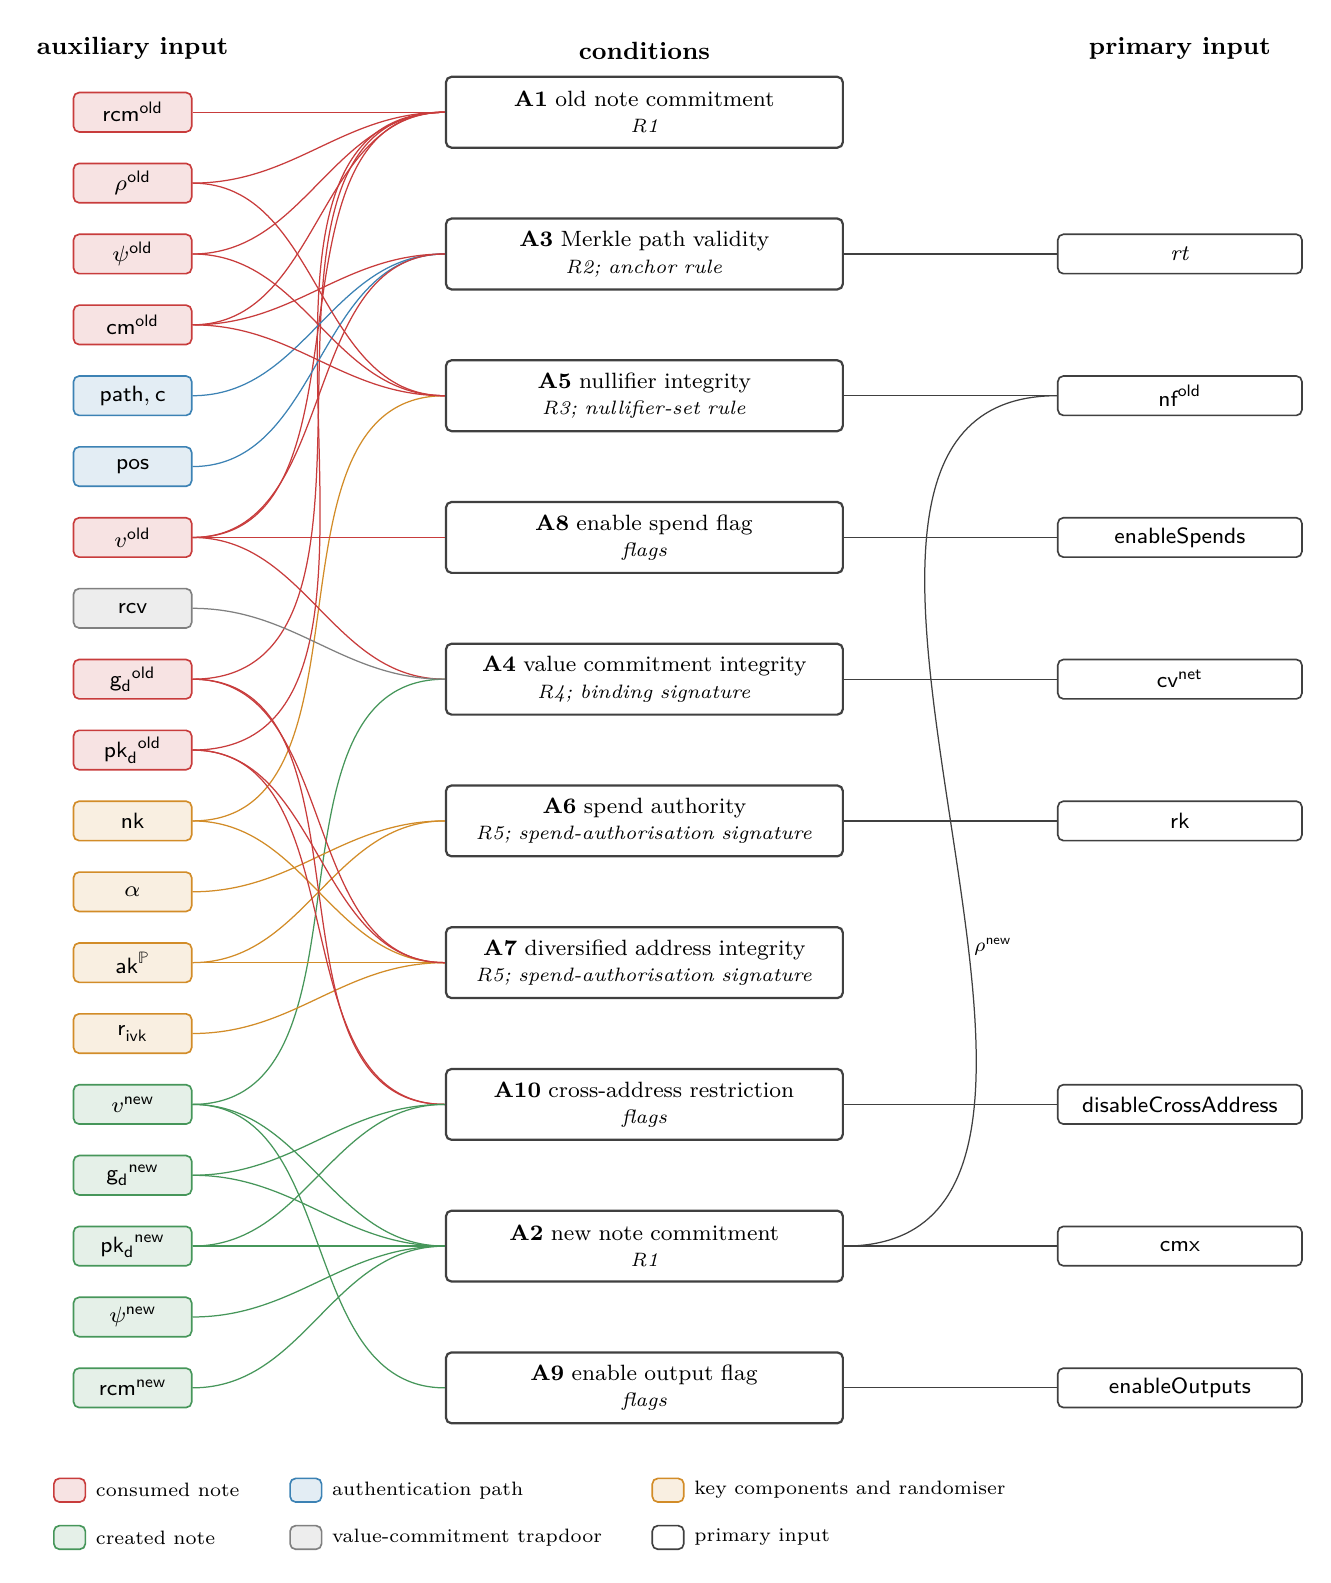
\begin{tikzpicture}[
  font=\footnotesize,
  ax/.style={draw=#1, fill=#1, fill opacity=0.14, text opacity=1,
    line width=0.6pt, rounded corners=2pt, inner sep=1.5pt,
    minimum height=5mm, minimum width=15mm},
  px/.style={draw=darkgray, line width=0.6pt, rounded corners=2pt,
    inner sep=1.5pt, minimum height=5mm, minimum width=31mm},
  cd/.style={draw=darkgray, line width=0.8pt, rounded corners=2pt,
    inner sep=2pt, text width=49mm, align=center, minimum height=9mm,
    fill=white},
  rd/.style={line width=0.45pt, draw=#1},
]
% auxiliary inputs
\node[ax=tierspend] (rcmo) at (0.8,0) {$\rcm^{\mathsf{old}}$};
\node[ax=tierspend] (rhoo) at (0.8,-0.9) {$\rho^{\mathsf{old}}$};
\node[ax=tierspend] (psio) at (0.8,-1.8) {$\psi^{\mathsf{old}}$};
\node[ax=tierspend] (cmo) at (0.8,-2.7) {$\cmsym^{\mathsf{old}}$};
\node[ax=tierin] (path) at (0.8,-3.6) {$\mathsf{path}, \mathsf{c}$};
\node[ax=tierin] (pos) at (0.8,-4.5) {$\mathsf{pos}$};
\node[ax=tierspend] (vo) at (0.8,-5.4) {$v^{\mathsf{old}}$};
\node[ax=gray] (rcv) at (0.8,-6.3) {$\rcv$};
\node[ax=tierspend] (gdo) at (0.8,-7.2) {$\gd^{\mathsf{old}}$};
\node[ax=tierspend] (pkdo) at (0.8,-8.1) {$\pkd^{\mathsf{old}}$};
\node[ax=tierfull] (nk) at (0.8,-9.0) {$\nksym$};
\node[ax=tierfull] (alpha) at (0.8,-9.9) {$\alpha$};
\node[ax=tierfull] (akP) at (0.8,-10.8) {$\aksym^{\PP}$};
\node[ax=tierfull] (rivk) at (0.8,-11.7) {$\rivk$};
\node[ax=tierrecv] (vn) at (0.8,-12.6) {$v^{\mathsf{new}}$};
\node[ax=tierrecv] (gdn) at (0.8,-13.5) {$\gd^{\mathsf{new}}$};
\node[ax=tierrecv] (pkdn) at (0.8,-14.4) {$\pkd^{\mathsf{new}}$};
\node[ax=tierrecv] (psin) at (0.8,-15.3) {$\psi^{\mathsf{new}}$};
\node[ax=tierrecv] (rcmn) at (0.8,-16.2) {$\rcm^{\mathsf{new}}$};
% conditions
\node[cd] (A1) at (7.3,0) {\textbf{A1} old note commitment\\
  {\scriptsize\itshape R1}};
\node[cd] (A3) at (7.3,-1.8) {\textbf{A3} Merkle path validity\\
  {\scriptsize\itshape R2; anchor rule}};
\node[cd] (A5) at (7.3,-3.6) {\textbf{A5} nullifier integrity\\
  {\scriptsize\itshape R3; nullifier-set rule}};
\node[cd] (A8) at (7.3,-5.4) {\textbf{A8} enable spend flag\\
  {\scriptsize\itshape flags}};
\node[cd] (A4) at (7.3,-7.2) {\textbf{A4} value commitment integrity\\
  {\scriptsize\itshape R4; binding signature}};
\node[cd] (A6) at (7.3,-9.0) {\textbf{A6} spend authority\\
  {\scriptsize\itshape R5; spend-authorisation signature}};
\node[cd] (A7) at (7.3,-10.8) {\textbf{A7} diversified address integrity\\
  {\scriptsize\itshape R5; spend-authorisation signature}};
\node[cd] (A10) at (7.3,-12.6) {\textbf{A10} cross-address restriction\\
  {\scriptsize\itshape flags}};
\node[cd] (A2) at (7.3,-14.4) {\textbf{A2} new note commitment\\
  {\scriptsize\itshape R1}};
\node[cd] (A9) at (7.3,-16.2) {\textbf{A9} enable output flag\\
  {\scriptsize\itshape flags}};
% primary inputs
\node[px] (rt) at (14.1,-1.8) {$\mathit{rt}$};
\node[px] (nf) at (14.1,-3.6) {$\nfsym^{\mathsf{old}}$};
\node[px] (es) at (14.1,-5.4) {$\mathsf{enableSpends}$};
\node[px] (cv) at (14.1,-7.2) {$\cvsym^{\mathsf{net}}$};
\node[px] (rk) at (14.1,-9.0) {$\rk$};
\node[px] (dca) at (14.1,-12.6) {$\mathsf{disableCrossAddress}$};
\node[px] (cmx) at (14.1,-14.4) {$\cmx$};
\node[px] (eo) at (14.1,-16.2) {$\mathsf{enableOutputs}$};
\node[font=\small\bfseries, anchor=south] at (0.8,0.55) {auxiliary input};
\node[font=\small\bfseries, anchor=south] at (7.3,0.55) {conditions};
\node[font=\small\bfseries, anchor=south] at (14.1,0.55) {primary input};
% edges from the auxiliary input
\foreach \s/\t/\c in {
    rcmo/A1/tierspend, rhoo/A1/tierspend, psio/A1/tierspend,
    cmo/A1/tierspend, vo/A1/tierspend, gdo/A1/tierspend, pkdo/A1/tierspend,
    path/A3/tierin, pos/A3/tierin, cmo/A3/tierspend, vo/A3/tierspend,
    nk/A5/tierfull, rhoo/A5/tierspend, psio/A5/tierspend, cmo/A5/tierspend,
    vo/A8/tierspend,
    vo/A4/tierspend, vn/A4/tierrecv, rcv/A4/gray,
    akP/A6/tierfull, alpha/A6/tierfull,
    akP/A7/tierfull, nk/A7/tierfull, rivk/A7/tierfull, gdo/A7/tierspend,
    pkdo/A7/tierspend,
    gdo/A10/tierspend, pkdo/A10/tierspend, gdn/A10/tierrecv,
    pkdn/A10/tierrecv,
    gdn/A2/tierrecv, pkdn/A2/tierrecv, vn/A2/tierrecv, psin/A2/tierrecv,
    rcmn/A2/tierrecv,
    vn/A9/tierrecv} {
  \draw[rd=\c] (\s.east) to[out=0, in=180] (\t.west);
}
% edges to the primary input
\foreach \s/\t in {A3/rt, A5/nf, A8/es, A4/cv, A6/rk, A10/dca, A2/cmx,
    A9/eo} {
  \draw[rd=darkgray] (\s.east) to[out=0, in=180] (\t.west);
}
\draw[rd=darkgray] (A2.east) to[out=0, in=180]
  node[pos=0.4, right, font=\scriptsize, inner sep=2pt]
  {$\rho^{\mathsf{new}}$} (nf.west);
% legend
\foreach \c/\t/\x/\y in {tierspend/consumed note/0.0/-17.5,
    tierin/authentication path/3.0/-17.5,
    tierfull/key components and randomiser/7.6/-17.5,
    tierrecv/created note/0.0/-18.1,
    gray/value-commitment trapdoor/3.0/-18.1} {
  \node[ax=\c, minimum width=4mm, minimum height=3mm, inner sep=0pt]
    (lg) at (\x,\y) {};
  \node[anchor=west, font=\scriptsize] at (lg.east) {\t};
}
\node[px, minimum width=4mm, minimum height=3mm, inner sep=0pt]
  (lg) at (7.6,-18.1) {};
\node[anchor=west, font=\scriptsize] at (lg.east) {primary input};
\end{tikzpicture}
\caption{The Action statement of Definition~\ref{def:action}. The auxiliary
input is on the left, coloured by group as in the legend; the primary input
is on the right; conditions A1 to A10 are in the centre, ordered by the side
of the Action they constrain rather than by number. Each condition has an
edge to every variable it reads; the edge from $\nfsym^{\mathsf{old}}$ to A2
carries $\rho^{\mathsf{new}} := \nfsym^{\mathsf{old}}$. Each condition is
tagged with the requirement of \S\ref{sec:intro-req} that it serves, or with
``flags'' for A8 to A10, and, where one exists, with the check outside the
proof that completes it: the anchor rule for A3, the nullifier-set rule for
A5, the binding signature for A4, and the spend-authorisation signature for
A6 and A7.}
\label{fig:action}
\end{figure}

\FloatBarrier
\subsection{The Action circuit and the Halo 2 proof}\label{sec:action-circuit}

The Action statement of Definition~\ref{def:action} is a relation and
prescribes no computation. The \emph{post-NU6.3 Action circuit} is one fixed
PLONKish circuit (\emph{Halo 2 Guide}, \S``PLONKish arithmetisation'') whose
constraints are designed to encode the typing and conditions A1 to A10; that
every satisfying assignment yields a witness of $\Rel_{\mathsf{Action}}$ is
part of Assumption~\ref{ass:ks} below. The same circuit serves every Action.
Its instance is the encoding of the eight primary inputs of
Definition~\ref{def:action}, bound to the proof as in the \emph{Halo 2
Guide}, \S``Instance columns and binding the public statement''; this
instance is the only Orchard-specific part of the proof system constructed in
this volume. Proofs are Halo~2 proofs (\emph{Halo 2 Guide}, \S``The Halo 2
proof system'' and \S``The complete Halo 2 protocol''; protocol
specification, \S``Zero-Knowledge Proving System''; ZIP 229, Abstract): a
PLONKish polynomial interactive oracle proof compiled with the inner-product
polynomial commitment and made non-interactive by the Fiat--Shamir
transform, with no trusted setup.

The circuit's native field is $\F_{p_{\Pallas}}$, the base field of the
Pallas group, so the Pallas point operations of A1 to A10 are arithmetic in
the native field. The proof's polynomial commitments lie in the Vesta group
$\G_{\Vesta}$, the group of points of the curve $y^2 = x^3 + 5$ over
$\F_{p_{\Vesta}}$, which has prime order $p_{\Pallas}$ (\S\ref{sec:prim-fields};
\emph{Math Guide}, \S``Base fields, scalar fields, and the Pasta cycle''); the
committed polynomials therefore have coefficients in $\F_{p_{\Pallas}}$. The
Pallas group carries the protocol's keys, commitments, signatures and note
encryption; the Vesta group carries only the proof's commitments.

The circuit has $2^{11}$ rows and a constraint-degree bound of $9$ across its
gates and its permutation and lookup identities (\emph{Halo 2 Guide},
\S``From statement to circuit: arithmetisation in practice''). Both are cited
constants; in this volume they enter only the Schwartz--Zippel term of the
first supporting analysis below.

Every Action of either pool, whatever it consumes or creates, dummy sides
included, is an instance of the same relation and circuit. The proofs of a
bundle's Actions are aggregated into one proof, encoded once per bundle,
which the verifier checks against the primary inputs of all the bundle's
Actions and the verifying key; each Action carries its own
spend-authorisation signature (protocol specification, \S``Action Transfers
and their Descriptions'' and \S``Action Descriptions'', note on proof
aggregation; ZIP 229, ``Transaction Format''). The verification procedure is
stated in ``Verification of a transaction'' (\S\ref{sec:tx-verify}).

Both pools use the post-NU6.3 circuit and its proving and verifying keys; the
pools are distinguished by their note commitment trees, nullifier sets, value
pool balances and component position in the transaction, not by circuits
(ZIP 229, Abstract, and Rationale, ``Reuse of the Orchard protocol with
minimal changes''). Consensus selects the Action verifying key by network
upgrade (protocol specification, \S``Action Descriptions'', consensus rules).
The key in force for every Action, in either pool and in version~$5$ and
version~$6$ transactions alike, is the post-NU6.3 verifying key, named by
upgrade and not by pool (ZIP 258, ``Consensus rules from~NU6.3
activation'').

\begin{assumption}[Discrete logarithms on Vesta]\label{ass:dl-vesta}
For every classical probabilistic polynomial-time algorithm, given a
generator $G$ of $\G_{\Vesta}$ and $[s]G$ for $s$ uniform in
$\F_{p_{\Pallas}}$, the probability of outputting $s$ is negligible
(\emph{Crypto Guide}, \S``Standing assumptions'', Remark ``Standing
assumptions for the sequel'', item~1, for the Vesta curve). Concretely, the
best known classical attack costs about $2^{126}$ group operations
(\emph{Crypto Guide}, \S``Instantiation on elliptic curves; the Pasta
curves'', Proposition ``The Pasta curves against the criteria''); the level
is cited, not recomputed. The volume uses this assumption only in the
extraction analysis of the inner-product commitment that supports
Assumption~\ref{ass:ks} (the second supporting analysis below).
\end{assumption}

\begin{assumption}[Knowledge soundness of the Action proof]\label{ass:ks}
Let the hash of the Fiat--Shamir transform of the proof system be modelled as
a random oracle. For every efficient adversary $\Adv$ that outputs primary
inputs $\mathsf{pub}_1, \dots, \mathsf{pub}_n$ and an aggregate proof $\pi$,
there is an efficient extractor $\Ext$, with access to $\Adv$ and to its
random-oracle queries, that outputs auxiliary inputs
$\mathsf{aux}_1, \dots, \mathsf{aux}_n$ such that the probability of the
event
\begin{gather*}
  \text{$\pi$ is accepted for $(\mathsf{pub}_1, \dots, \mathsf{pub}_n)$
    under the post-NU6.3 verifying key} \\
  \text{and } (\mathsf{pub}_i, \mathsf{aux}_i) \notin
    \Rel_{\mathsf{Action}} \text{ for some } i
\end{gather*}
is negligible. This is the knowledge-soundness clause of the \emph{Crypto
Guide}'s Definition ``SNARK'' (\S``SNARKs: succinct non-interactive
arguments of knowledge'') for the relation $\Rel_{\mathsf{Action}}$ of
Definition~\ref{def:action}. It includes that every satisfying assignment of
the post-NU6.3 circuit yields a witness of $\Rel_{\mathsf{Action}}$, for
which the specification requires canonical decompositions of the scalar of
A5 and of the scalar $\ivk$ in $[\ivk]\,\gd^{\mathsf{old}}$ (protocol
specification, \S``Action Statement (Orchard)'', note on canonical scalar
decompositions).
\end{assumption}

Assumption~\ref{ass:ks} is an assumption, not a proved result. Its status is
designed but unspecified: bounds exist for the analysed protocol, and no
theorem carries them to the deployed Fiat--Shamir-compiled protocol
(\emph{Halo 2 Guide}, \S``The algebraic group model''). The volume assumes
the property, proves no bound and asserts no loss factor. The two supporting
analyses that follow are cited, not re-proved, and not combined into a bound.

% compute/fields.py:
% [sec:action-circuit] Schwartz--Zippel term deg D/|F| at n = 2^11 rows,
%   degree bound 9, F = F_p_Pallas: deg D < 9 * 2^11 = 18432,
%   term < 18432/p_Pallas = 2^-239.83 < 2^-239
%   (Halo 2 Guide: 'around 2^-240')
\begin{remark}[Supporting analysis (i): a Schwartz--Zippel term]
A non-zero gap polynomial $D$ over $\F_{p_{\Pallas}}$, fixed by the prover's
commitments before the challenge is drawn, vanishes at a uniform challenge
with probability at most $\deg D / p_{\Pallas}$ (\emph{Halo 2 Guide},
\S``Why checking one random point is a proof''). At the Orchard parameters,
$2^{11}$ rows and constraint-degree bound $9$, the constraint expression has
degree below $9 \cdot 2^{11}$, and so does the committed quotient, of $8$
chunks of degree below $2^{11}$, times the vanishing polynomial of degree
$2^{11}$ (\emph{Halo 2 Guide}, \S``The complete Halo 2 protocol'',
Phase~4). Hence $\deg D < 9 \cdot 2^{11} = 18432$, and the term is below
$18432 / p_{\Pallas} < 2^{-239}$. The term bounds one check at one challenge
and is not a security level of the proof: the complete protocol has further
randomised checks, and under the Fiat--Shamir transform an adversary may
retry challenges, one hash query per retry (\emph{Halo 2 Guide},
\S``Removing the verifier: the Fiat--Shamir transform'').
\end{remark}

\begin{remark}[Supporting analysis (ii): extraction for the inner-product
commitment]
The inner-product polynomial commitment, whose commitments lie in
$\G_{\Vesta}$, has an interactive opening protocol that is knowledge-sound
under the discrete-logarithm assumption in that group,
Assumption~\ref{ass:dl-vesta}, with an expected-polynomial-time tree
extractor (\emph{Halo 2 Guide}, \S``The inner-product polynomial
commitment'', Theorem ``Knowledge soundness of IPA''). The
Fiat--Shamir-compiled argument inherits the interactive extraction bound only
up to a loss in the adversary's random-oracle query count (same theorem;
\S``Removing the verifier: the Fiat--Shamir transform''), and the tighter
analyses in the algebraic group model are proved for the analysed protocol,
not for the deployed transcript (\S``The algebraic group model''). No loss
factor is asserted.
\end{remark}

\begin{assumption}[Zero knowledge of the Action proof]\label{ass:zk}
Let the hash of the Fiat--Shamir transform be modelled as a programmable
random oracle. There is an efficient simulator that, given only the primary
inputs $\mathsf{pub}_1, \dots, \mathsf{pub}_n$ of a bundle and programming
the random oracle, outputs an aggregate proof whose distribution is
statistically indistinguishable from that of an honestly generated proof for
any $\mathsf{aux}_1, \dots, \mathsf{aux}_n$ with
$(\mathsf{pub}_i, \mathsf{aux}_i) \in \Rel_{\mathsf{Action}}$ for every $i$:
every distinguisher that makes polynomially many random-oracle queries,
whatever its running time, has negligible advantage. This is zero knowledge
of statistical grade in the non-interactive, random-oracle form of the
\emph{Crypto Guide}'s Definition ``Zero knowledge'' (\S``The simulation
paradigm and zero knowledge'').
\end{assumption}

Assumption~\ref{ass:zk} is an assumption, not a proved result. The
\emph{Halo 2 Guide}, \S``Zero knowledge: hiding the witness in Halo 2'',
records honest-verifier zero knowledge of the interactive protocol and zero
knowledge of its Fiat--Shamir compilation in the programmable random-oracle
model, subject to its composition and Fiat--Shamir hypotheses, without
reproving it. Assumptions~\ref{ass:ks} and~\ref{ass:zk} are the two
assumptions on the Action proof that ``Security'' (\S\ref{sec:security})
composes with the propositions of the preceding sections.

\section{Note encryption}\label{sec:enc}

This section constructs the in-band delivery of a created note: its
plaintext, its encryption to the recipient by one-shot Diffie--Hellman on the
diversified base, the outgoing ciphertext keyed from $\ovk$ and the Action's
own public fields, and the trial decryption and acceptance checks by which a
recipient obtains a note consistent with the published $\cmx$. It states the
two assumptions that note encryption adds, proves decryption correctness,
confidentiality and key privacy of the encryption to the recipient,
confidentiality of the outgoing ciphertext, and the consistency of accepted
notes, and states what each key tier can decrypt.

\subsection{The note plaintext}\label{sec:enc-plaintext}

Every Action carries, beside the extracted commitment $\cmx$ of its created
note, a \emph{note ciphertext} $(\mathsf{epk}^{\star}, C_{\mathsf{enc}},
C_{\mathsf{out}})$. The component $C_{\mathsf{enc}}$ encrypts the plaintext of
the created note so that the holder of the recipient's incoming viewing key
$\ivk$ recovers the note and its memo from the chain alone (protocol
specification, \S``In-band secret distribution (Sapling and Orchard)'' and
\S``Action Descriptions''). The component $C_{\mathsf{out}}$ lets the sender,
or any party that holds the outgoing viewing key $\ovk$ under which it was
formed, recover the same plaintext (\S\ref{sec:enc-out}). The fields
$\mathsf{epk}^{\star}$, $C_{\mathsf{enc}}$ and $C_{\mathsf{out}}$ are not
inputs of the Action statement (Definition~\ref{def:action}), which therefore
does not constrain them; the checks that make a decrypted note consistent
with $\cmx$ are made by the recipient (\S\ref{sec:enc-trial}).

% compute/encodings.py:
% [sec:enc-plaintext] note plaintext = 1 (lead byte) + 11 (d) + 8 (v)
%   + 32 (rseed) + 512 (memo) = 564 bytes
\begin{definition}[Note plaintext]
Let a created note have recipient address $(d, \pkd)$ and value
$v \in \{0, \dots, 2^{64} - 1\}$. Its \emph{note plaintext} is the tuple
$\mathsf{np} := (\mathsf{leadByte}, d, v, \mathsf{rseed}, \mathsf{memo})$,
encoded as the byte string
\[
  \mathsf{leadByte} \,\|\, \mathsf{LEBS2OSP}_{88}(d) \,\|\,
  \mathsf{I2LEOSP}_{64}(v) \,\|\, \mathsf{rseed} \,\|\, \mathsf{memo},
\]
where $\mathsf{leadByte}$ is one byte, the format version of ``The note
seed'' (\S\ref{sec:notes-seed}), equal to $\mathtt{0x03}$ for an
Ironwood-pool output; $d$ is the $88$-bit diversifier of the address
($11$ bytes); $v$ occupies $8$ bytes; $\mathsf{rseed}$ is the $32$-byte note
seed; and $\mathsf{memo}$ is a $512$-byte string chosen by the sender, whose
use is by agreement between sender and recipient (protocol specification,
\S``Note Plaintexts and Memo Fields'' and \S``Encodings of Note Plaintexts
and Memo Fields''). The encoding has the fixed length
$1 + 11 + 8 + 32 + 512 = 564$ bytes, so the length of a ciphertext carries
no information about the plaintext.
\end{definition}

The plaintext omits $\pkd$, $\rho$, $\psi$ and $\rcm$. The recipient
computes $\pkd = [\ivk]\,\gd$, takes $\rho = \nfsym^{\mathsf{old}}$ from the
same Action (``Nullifier chaining'', \S\ref{sec:nf-chaining}), and derives
$\psi$ and $\rcm$ from $\mathsf{rseed}$ (\S\ref{sec:notes-seed}).

For each output the sender draws $\mathsf{rseed}$ uniformly from the $32$-byte
strings, independently of every other output. The ephemeral secret key of
this section is
\[
  \mathsf{esk} = \mathrm{ToScalar}\bigl(\mathsf{PRFexpand}_{\mathsf{rseed}}
    ([\mathtt{0x04}] \,\|\, \mathsf{I2LEOSP}_{256}(\nfsym^{\mathsf{old}}))
  \bigr),
\]
derived in ``The note seed'' (\S\ref{sec:notes-seed}) together with $\psi$
and $\rcm$. The sender redraws $\mathsf{rseed}$ when $\mathsf{esk} = 0$ or
$\cmx = \bot$, so $\mathsf{esk} \in \F_{p_{\Vesta}}^{*}$ (protocol
specification, \S``Sending Notes (Orchard)''; ZIP 2005, ``Changes to the
Protocol Specification'', \S 4.7.3).

\FloatBarrier
\subsection{Encryption to the recipient}\label{sec:enc-encrypt}

% compute/encodings.py:
% [sec:enc-encrypt] C_enc = 564 + 16 (AEAD tag) = 580 bytes
\begin{construction}[Encryption to the recipient]
Let $(d, \pkd)$ be the recipient's address, $\gd = \mathsf{DiversifyHash}(d)$
its diversified base (``Diversified addresses'', \S\ref{sec:keys-addr}), and
$\mathsf{esk}$ as in \S\ref{sec:enc-plaintext}. A star encoding
$P^{\star}$ enters a byte string as the $32$ bytes
$\mathsf{LEBS2OSP}_{256}(P^{\star})$ (\S\ref{sec:prim-fields}), with which it
is identified below. The sender computes the \emph{ephemeral
public key}, the \emph{shared secret} and the \emph{encryption key}
\begin{align*}
  \mathsf{epk} &:= [\mathsf{esk}]\,\gd, \qquad
  s := [\mathsf{esk}]\,\pkd, \\
  K_{\mathsf{enc}} &:= \mathsf{KDF}(s, \mathsf{epk}) :=
    \mathrm{BLAKE2b\text{-}256}\bigl(\texttt{Zcash\_OrchardKDF},\
    s^{\star} \,\|\, \mathsf{epk}^{\star}\bigr),
\end{align*}
with $\mathrm{BLAKE2b\text{-}256}(P, x)$ unkeyed BLAKE2b with a $32$-byte
output and the $16$-byte personalisation $P$, and the ciphertext
$C_{\mathsf{enc}} := \mathsf{Enc}_{K_{\mathsf{enc}}}(\mathsf{np})$. The pair
$\mathsf{Enc}_K$, $\mathsf{Dec}_K$ denotes ChaCha20-Poly1305 encryption and
decryption under the $256$-bit key $K$ with the all-zero $96$-bit nonce and
empty associated data; decryption returns $\bot$ when the tag does not
verify (\emph{Crypto Guide}, \S``The ChaCha20-Poly1305 AEAD'', Construction
``ChaCha20-Poly1305''). The Action publishes the $32$-byte field
$\mathsf{epk}^{\star}$ and $C_{\mathsf{enc}}$, of $564 + 16 = 580$ bytes,
the plaintext and the $16$-byte tag (protocol specification,
\S``Encryption (Sapling and Orchard)'', \S``Orchard Key Agreement'',
\S``Orchard Key Derivation'' and
\href{https://zips.z.cash/protocol/protocol.pdf#concretesym}%
{\S``Symmetric Encryption''}).
\end{construction}

The key agreement is Diffie--Hellman on Pallas: public keys are non-identity
points, private keys lie in $\F_{p_{\Vesta}}^{*}$, and both the derivation of
a public key from a base and the agreement are scalar multiplication
(protocol specification, \S``Orchard Key Agreement''). A consensus rule
requires $\mathsf{epk}^{\star}$ to be the canonical encoding of a
non-identity Pallas point (protocol specification, \S``Action
Descriptions''). The fixed nonce is safe because every key encrypts once:
$K_{\mathsf{enc}}$ depends on the fresh $\mathsf{esk}$ of its output, and the
key of $C_{\mathsf{out}}$ is derived separately (\S\ref{sec:enc-out}). The
scheme is the \emph{Crypto Guide}'s Construction ``DH-based hybrid
public-key encryption'' (\S``Hybrid public-key encryption'') over the
per-address base $\gd$ in place of a fixed generator, as the same volume
records for deployed note delivery (\S``Shielded-note delivery as deployed
hybrid encryption'').

\begin{proposition}[Decryption correctness]\label{prop:dec-correct}
Let $(d, \pkd)$ be an address of the incoming viewing key $\ivk$, so
$\pkd = [\ivk]\,\gd$ (\S\ref{sec:keys-addr}), and let
$\mathsf{epk} = [\mathsf{esk}]\,\gd$ with
$\mathsf{esk} \in \F_{p_{\Vesta}}^{*}$. Then
\[
  [\ivk]\,\mathsf{epk} = [\mathsf{esk}]\,\pkd = s .
\]
Hence the holder of $\ivk$ computes
$K_{\mathsf{enc}} = \mathsf{KDF}([\ivk]\,\mathsf{epk}, \mathsf{epk})$ from the
published $\mathsf{epk}^{\star}$ and obtains
$\mathsf{Dec}_{K_{\mathsf{enc}}}(C_{\mathsf{enc}}) = \mathsf{np}$, and a party
that knows $(\pkd, \mathsf{esk})$ obtains the same shared secret as
$[\mathsf{esk}]\,\pkd$.
\end{proposition}

\begin{proof}
In the cyclic Pallas group $[a]([b]\,P) = [ab]\,P = [b]([a]\,P)$, so
$[\ivk]([\mathsf{esk}]\,\gd) = [\mathsf{esk}]([\ivk]\,\gd) =
[\mathsf{esk}]\,\pkd$. The recipient decodes
$\mathsf{epk} = \mathsf{abst}_{\PP}(\mathsf{epk}^{\star})$, and because the
star encoding is canonical (\S\ref{sec:prim-fields}) it re-encodes to the
published bytes. The function
$\mathsf{KDF}$ is deterministic and both parties apply it to
$(s^{\star}, \mathsf{epk}^{\star})$, so they derive the same
$K_{\mathsf{enc}}$; correctness of ChaCha20-Poly1305 gives
$\mathsf{Dec}_{K_{\mathsf{enc}}}(\mathsf{Enc}_{K_{\mathsf{enc}}}(\mathsf{np}))
= \mathsf{np}$. This is the \emph{Crypto Guide}'s Theorem ``Correctness of
hybrid encryption'' (\S``Hybrid public-key encryption'') over the base
$\gd$.
\end{proof}

\begin{assumption}[The note-encryption hashes as random oracles]%
\label{ass:kdf}
In security arguments the key-derivation function $\mathsf{KDF}$
(BLAKE2b-256 personalised $\texttt{Zcash\_OrchardKDF}$), the function
$\mathsf{PRF}^{\mathsf{ock}}$ (BLAKE2b-256 personalised
$\texttt{Zcash\_Orchardock}$, constructed in \S\ref{sec:enc-out}), and
$\mathsf{PRFexpand}$ on inputs with leading byte $\mathtt{0x04}$, the
derivation of $\mathsf{esk}$ from $\mathsf{rseed}$, are modelled as
independent random oracles (\emph{Crypto Guide}, \S``The random oracle
model'', Definition ``Random oracle''). The PRF assumption
(Assumption~\ref{ass:prf-expand}) does not suffice for the last: it requires
a key unknown to the adversary, whereas the plaintext that $K_{\mathsf{enc}}$
encrypts contains $\mathsf{rseed}$, the key from which $\mathsf{esk}$, and
hence $K_{\mathsf{enc}}$, is derived. On its other inputs
$\mathsf{PRFexpand}$ is used only under Assumption~\ref{ass:prf-expand}. The
assumption is a heuristic about BLAKE2b, not a theorem; every result that
uses $\mathsf{KDF}$, $\mathsf{PRF}^{\mathsf{ock}}$ or the derivation of
$\mathsf{esk}$ names it.
\end{assumption}

\begin{assumption}[Confidentiality and integrity of ChaCha20-Poly1305]%
\label{ass:aead}
For a uniform $256$-bit key that encrypts a single plaintext,
ChaCha20-Poly1305 with the all-zero nonce and empty associated data is
\begin{enumerate}
\item[(a)] \emph{confidential}: the encryptions of any two plaintexts of
  equal length are computationally indistinguishable; and
\item[(b)] \emph{integral}: no efficient adversary without the key outputs a
  ciphertext, other than one it was given, that decrypts to a value other
  than $\bot$.
\end{enumerate}
The \emph{Crypto Guide}'s Theorem ``Security of ChaCha20-Poly1305''
(\S``The ChaCha20-Poly1305 AEAD'') derives both, with explicit bounds, from
the pseudorandomness of ChaCha20. The protocol specification requires
one-time INT-CTXT and IND-CPA security of the scheme, properties~(b)
and~(a) above (\emph{Crypto Guide}, Definitions ``Ciphertext integrity,
INT-CTXT'' and ``CPA security'', \S``Authenticated encryption with
associated data'' and \S``Chosen-plaintext security''; protocol
specification,
\href{https://zips.z.cash/protocol/protocol.pdf#abstractsym}%
{\S``Symmetric Encryption''}). The scheme is not
key-committing: a party that chooses two keys can construct one ciphertext
that decrypts validly under both (\emph{Crypto Guide}, \S``The
ChaCha20-Poly1305 AEAD'', Remark ``Wrong-key rejection and key
commitment''). No result of this volume relies on the tag against a sender
who chooses the key.
\end{assumption}

% compute/fields.py:
% [sec:keys-capabilities] x-coordinates of non-identity Pallas points:
%   (p_Vesta - 1)/2 elements, all < p_Pallas < p_Vesta
% [sec:keys-capabilities] uniform exponent mod p_Vesta lies in that set
%   with probability (p_Vesta - 1)/(2 p_Vesta) = 1/2 - 1/(2 p_Vesta);
%   loss factor 2 p_Vesta/(p_Vesta - 1) = 2 + 2/(p_Vesta - 1)
% [sec:prim-prf] ToScalar (mod p_Vesta): Math Guide bound m/2^512
%   = 2^-258 (1 + e), 0 < e < 2^-128, so < 2^-257
\begin{proposition}[Confidentiality and key privacy of note encryption]%
\label{prop:enc-privacy}
Let a key be generated honestly with $\mathsf{use\_qsk} = \mathsf{false}$. An
efficient adversary receives the address $(d, \pkd)$ of the key at an index
of its choice and data $z$ that an efficient algorithm computes independently
of the key and of $\mathsf{rseed}$; it chooses a value $v$, a memo and
$\rho \in \F_{p_{\Pallas}}$. An output to $(d, \pkd)$ with these values and
$\rho = \nfsym^{\mathsf{old}}$ is formed as in \S\ref{sec:enc-plaintext} and
the construction above, with $\mathsf{rseed}$ uniform, and $\cmx$ is the
extracted commitment of its note. Then the triple
$(\mathsf{epk}^{\star}, C_{\mathsf{enc}}, \cmx)$ is computationally
indistinguishable from $(E^{\star}, C', \cmx)$, where $E$ is a uniform
non-identity Pallas point and $C'$ is the encryption of a fixed $564$-byte
string under an independent uniform key. The hypotheses are
Assumptions~\ref{ass:ddh-pallas}, \ref{ass:kdf}, \ref{ass:aead},
\ref{ass:grouphash-ro} (for $\gd$), \ref{ass:vk-hiding} (for the joint
distribution of $\ivk$ and $d$) and~\ref{ass:prf-expand} (for the dependence
of $\cmx$ on $\mathsf{rseed}$), together with Assumption~\ref{ass:dl-pallas}
for Lemma ``Rejection in key generation'' (\S\ref{sec:keys-viewing}).
\end{proposition}

Since $E$ and $C'$ are computed from neither the plaintext nor the address,
the pair $(\mathsf{epk}^{\star}, C_{\mathsf{enc}})$ reveals neither the
plaintext, $\mathsf{rseed}$ included, nor the recipient's address: given two
addresses of independent keys, the data $z$ may contain the second, and the
ciphertext is indistinguishable from one independent of both. The value
$\cmx$ is included so that the result applies within an Action. Of the
hypotheses only Assumption~\ref{ass:ddh-pallas}, used through the
computational Diffie--Hellman problem that it implies, concerns the one-shot
key agreement between $\mathsf{esk}$ and $\pkd$; Assumptions~\ref{ass:kdf}
and~\ref{ass:aead} concern the hash functions and the cipher. The adversary
is passive: the volume does not claim indistinguishability of encryptions
against an adversary that may also obtain decryptions of ciphertexts of its
choice other than the challenge, before and after receiving it (IND-CCA2),
which the protocol specification, \S``Key Derivation'', requires of the
scheme.

\begin{proof}
The proof is a sequence of games (\emph{Crypto Guide}, \S``Security as a
game'', Remark ``Game-hopping''); each reduction below runs the adversary
and the rest of the game. Let $Q$ be the event that the adversary queries
the oracle of Assumption~\ref{ass:kdf} for $\mathsf{PRFexpand}$ at an input
keyed by $\mathsf{rseed}$.

\emph{Preliminary step.} As in the proof of
Proposition~\ref{prop:capabilities}, the key is replaced by a single draw
without rejection and its triple $(\ask, \nksym, \rivk)$ by independent
uniform elements (Lemma~\ref{lem:prf-independence},
Assumption~\ref{ass:prf-expand}; Lemma ``Rejection in key generation'',
\S\ref{sec:keys-viewing}, Assumptions~\ref{ass:dl-pallas}
and~\ref{ass:grouphash-ro}). Then $(\ivk, \dk)$ is replaced by
$(\CommitIvk_{\rivk'}(\aksym, \nksym), u_1)$
(Assumption~\ref{ass:vk-hiding}; the reduction draws $\ask$ and $\nksym$
itself). Now $d = \mathsf{FF1\text{-}AES256}_{u_1}(\mathrm{LE}_{88}(j))$, and
$\ivk$ is, independently of $d$, $0$ with probability $1/p_{\Vesta}$ and
otherwise uniform on the set $X_{\Pallas}$ of $x$-coordinates of
non-identity points, of $(p_{\Vesta} - 1)/2$ elements, except on the
negligible event $\hat{M} = \bot$ (Lemma ``Distribution of $\ivk$'',
\S\ref{sec:keys-viewing}). The redraw of $\mathsf{rseed}$ is replaced by a
single trial, at the cost of the redraw probability, negligible as in the
proof of Proposition~\ref{prop:cm-derived}.

(1)~By Assumption~\ref{ass:kdf}, $\mathsf{esk}$ is $\mathrm{ToScalar}$ of a
random-oracle output at an input keyed by $\mathsf{rseed}$. It is replaced by
an independent uniform element of $\F_{p_{\Vesta}}^{*}$. The oracle's value
at that input is used nowhere else, so the games are identical until $Q$
occurs; they differ by at most $\Pr[Q]$ in the new game plus the reduction
distance of $\mathrm{ToScalar}$, below $2^{-257}$, and $1/p_{\Vesta}$ for
the value $0$ (\emph{Crypto Guide}, \S``Security as a game'', Remark
``Game-hopping''; \S\ref{sec:prim-prf}).

(2)~The key $K_{\mathsf{enc}}$ is replaced by an independent uniform key.
The games differ only on the event $C$ that the adversary queries the
$\mathsf{KDF}$ oracle at $s^{\star} \,\|\, \mathsf{epk}^{\star}$, and
$s = [\mathsf{esk}]\,\pkd$ solves the computational Diffie--Hellman instance
$(\gd, \pkd, \mathsf{epk})$. This is the game hop of the \emph{Crypto
Guide}'s Theorem ``Passive security of hybrid encryption'' (\S``Hybrid
public-key encryption''), with loss factor the number $q_K$ of
$\mathsf{KDF}$ queries, run over $\gd$. A distinguisher
$\mathcal{D}$ for Assumption~\ref{ass:ddh-pallas} receives
$([a]\,P, [b]\,P, [c]\,P)$ with $a$ uniform on $X_{\Pallas}$ and $b, c$
uniform. It answers each new query of $\GroupHash$ under the domain
$\texttt{z.cash:Orchard-gd}$ with $[t]\,P$ for a fresh uniform $t$,
recorded, a uniform point as in the model of
Assumption~\ref{ass:grouphash-ro}, so that $\gd = [t]\,P$ with $t$ known. It
sets $\pkd := [t]([a]\,P) = [a]\,\gd$, which embeds $a$ as $\ivk$, and
$\mathsf{epk} := [t]([b]\,P) = [b]\,\gd$, which embeds $b$ as
$\mathsf{esk}$; it draws $u_1$ and $\mathsf{rseed}$, computes $d$, $\cmx$ and
$C_{\mathsf{enc}}$ under a uniform key itself, and answers the other oracles
lazily. It then decodes the first $32$ bytes of a uniformly chosen
$\mathsf{KDF}$ query to a point $S$ and outputs $1$ exactly when
$S = [t]([c]\,P)$. The simulation differs from the game only when
$\ivk = 0$ in the game, or $b = 0$ or $t = 0$ in the simulation, of total
probability at most $3/p_{\Vesta}$. On a Diffie--Hellman triple
$\mathcal{D}$ therefore outputs $1$ with probability at least
$\Pr[C]/q_K - 3/p_{\Vesta}$; on a random triple the point $[t]([c]\,P)$ is,
for $t \neq 0$, uniform and independent of the view, and $\mathcal{D}$
outputs $1$ with probability at most $4/p_{\Vesta}$. An algorithm that
computes Diffie--Hellman secrets on Pallas thus decides DDH, and
$\Pr[C] \le q_K\,(\epsilon_{\mathcal{D}} + 7/p_{\Vesta})$ for the advantage
$\epsilon_{\mathcal{D}}$ of $\mathcal{D}$. The exponent embedded as $\ivk$ is
uniform on $X_{\Pallas}$ in Assumption~\ref{ass:ddh-pallas}. Against the
computational Diffie--Hellman problem with a uniform exponent on
$\F_{p_{\Vesta}}$, which lies in $X_{\Pallas}$ with probability
$(p_{\Vesta} - 1)/(2 p_{\Vesta})$ and on those instances gives an exact
simulation, the same reduction loses a factor
$2 p_{\Vesta}/(p_{\Vesta} - 1)$, about $2$ (proof of
Proposition~\ref{prop:capabilities}, part~(d)).

(3)~Now $\mathsf{epk} = [\mathsf{esk}]\,\gd$ with $\mathsf{esk}$ uniform on
$\F_{p_{\Vesta}}^{*}$ is a uniform non-identity point for every generator
$\gd$, and the $\mathsf{KDF}$ context contains no key of the recipient
(\emph{Crypto Guide}, \S``Key privacy'', Remark ``What key privacy buys
upstairs''). The ciphertext $C_{\mathsf{enc}}$ is an encryption under a
uniform key used once, and Assumption~\ref{ass:aead}(a) replaces
$\mathsf{np}$ by the fixed string; the reduction obtains $C_{\mathsf{enc}}$
from its challenger and computes the rest. The last game outputs
$(E^{\star}, C', \cmx)$.

(4)~In the last game $\mathsf{rseed}$ enters the view only through $\cmx$,
that is through $\mathsf{PRFexpand}_{\mathsf{rseed}}$ under the leading bytes
$\mathtt{0x09}$ and $\mathtt{0x0B}$. A distinguisher with oracle access to
$\mathsf{PRFexpand}_{\mathsf{rseed}}$ or to a random function computes $\cmx$
from its oracle, runs the adversary, and outputs $1$ when some key $k$ of a
query at a leading byte $\mathtt{0x04}$ satisfies
$\mathsf{PRFexpand}_k([\mathtt{0x09}] \,\|\, \mathsf{I2LEOSP}_{256}(\rho))$
equal to its oracle's answer at that input. It outputs $1$ with probability
at least $\Pr[Q]$ in the first case. In the second the view depends on that
answer only through $\cmx$, and the trapdoor $\rcm$, $\mathrm{ToScalar}$ of
the independent answer at the $\mathtt{0x0B}$ input, is within $2^{-257}$ of
uniform; by Proposition~\ref{prop:cm}(a), $\cmx$ is therefore independent of
that answer up to $2^{-257} + \epsilon_{\bot}$, for $\epsilon_{\bot}$ the
probability that the hash point of $M(n)$ is $\bot$, negligible as in the
proof of Proposition~\ref{prop:cm-derived}. The distinguisher thus outputs
$1$ with probability at most $q \cdot 2^{-512} + 2^{-257} + \epsilon_{\bot}$,
for $q$ such queries, and $\Pr[Q]$ in the last game is negligible
under Assumption~\ref{ass:prf-expand} (with
Lemma~\ref{lem:prf-independence}). Every reduction of hops~(2) and~(3) draws
$\mathsf{rseed}$ itself and detects $Q$, so each hop changes the probability
of $Q$ by at most its own cost. Hence $\Pr[Q]$ is negligible in the game of
hop~(1) as well, and the sum of the costs of all hops is negligible.

The DDH hybrid of the \emph{Crypto Guide}'s Theorem ``ElGamal is key-private
under DDH'' (\S``Key privacy'') is not used: as stated it embeds a uniform
exponent of $\F_{p_{\Vesta}}$ as the recipient's key, whereas $\ivk$ is not
uniform on $\F_{p_{\Vesta}}$; and the factor-$2$ argument above transfers a
search problem such as computational Diffie--Hellman, not a decision
problem, since on instances outside $X_{\Pallas}$ a distinguisher's output
is unconstrained.
\end{proof}

\FloatBarrier
\subsection{The outgoing ciphertext}\label{sec:enc-out}

% compute/encodings.py:
% [sec:enc-out] C_out = 32 (pk_d*) + 32 (esk) + 16 = 80 bytes
% compute/OUTPUT.md, cited numbers:
% out-plaintext (l_P + 256)/8 = 64 bytes: spec 'Encryption (Sapling and
%   Orchard)'
\begin{construction}[Outgoing ciphertext]
The sender chooses an outgoing viewing key $\ovk$ of its own, such as that of
the address whose note the Action consumes (``Viewing keys'',
\S\ref{sec:keys-viewing}), or $\ovk = \bot$. If $\ovk \neq \bot$, the
\emph{outgoing cipher key} is
\begin{align*}
  \mathsf{ock} &:= \mathsf{PRF}^{\mathsf{ock}}_{\ovk}(\cvsym^{\mathsf{net}},
    \cmx, \mathsf{epk}) \\
  &:= \mathrm{BLAKE2b\text{-}256}\bigl(\texttt{Zcash\_Orchardock},\
    \ovk \,\|\, (\cvsym^{\mathsf{net}})^{\star} \,\|\,
    \mathsf{I2LEOSP}_{256}(\cmx) \,\|\, \mathsf{epk}^{\star}\bigr),
\end{align*}
where $\cvsym^{\mathsf{net}}$ is the Action's net value commitment
(Definition~\ref{def:cv-net}) and $\cmx$ its extracted note commitment
(Definition~\ref{def:notecommit}), and the \emph{outgoing plaintext} is the
$32 + 32 = 64$-byte string
$\mathsf{op} := \pkd^{\star} \,\|\, \mathsf{I2LEOSP}_{256}(\mathsf{esk})$.
If $\ovk = \bot$, the sender draws $\mathsf{ock}$ uniformly from the
$256$-bit strings and $\mathsf{op}$ uniformly from the $64$-byte strings. In
both cases $C_{\mathsf{out}} := \mathsf{Enc}_{\mathsf{ock}}(\mathsf{op})$, of
$64 + 16 = 80$ bytes, and the Action publishes it; with $\ovk = \bot$ no
outgoing viewing key recovers it (protocol specification, \S``Encryption
(Sapling and Orchard)'', \S``Sending Notes (Orchard)'' and
\href{https://zips.z.cash/protocol/protocol.pdf#concreteprfs}%
{\S``Pseudo Random Functions''}).
\end{construction}

\begin{construction}[Recovery with $\ovk$]
For an Ironwood-pool output, the holder of $\ovk$
\begin{enumerate}[label=(\roman*)]
\item computes $\mathsf{ock}$ from $\ovk$ and the Action's public
  $\cvsym^{\mathsf{net}}$, $\cmx$ and $\mathsf{epk}^{\star}$, and
  decrypts $C_{\mathsf{out}}$ under $\mathsf{ock}$ to the outgoing plaintext
  $\mathsf{op}$, rejecting $\bot$;
\item parses $\mathsf{op}$ as a $32$-byte string $b_1$ followed by a
  $32$-byte string $b_2$, and reads $\mathsf{esk}$ as the integer
  $\mathsf{LEOS2IP}_{256}(b_2)$, rejecting $\mathsf{esk} \ge p_{\Vesta}$, and
  $\pkd$ as the point $\mathsf{abst}_{\PP}(b_1)$, rejecting $\bot$ and
  $\mathcal{O}$;
\item computes $s := [\mathsf{esk}]\,\pkd$,
  $K_{\mathsf{enc}} := \mathsf{KDF}(s, \mathsf{epk})$ and
  $\mathsf{np} := \mathsf{Dec}_{K_{\mathsf{enc}}}(C_{\mathsf{enc}})$,
  rejecting $\bot$;
\item rejects unless $\mathsf{leadByte} = \mathtt{0x03}$;
\item with $\rho := \nfsym^{\mathsf{old}}$ of the same Action, rejects unless
  \[
    \mathsf{esk} = \mathrm{ToScalar}\bigl(\mathsf{PRFexpand}_{\mathsf{rseed}}
    ([\mathtt{0x04}] \,\|\, \mathsf{I2LEOSP}_{256}(\rho))\bigr);
  \]
\item computes $\gd := \mathsf{DiversifyHash}(d)$, then $\psi$, then $\rcm$
  under $\mathtt{0x03}$ from $\gd$, $\pkd$, $v$, $\rho$ and $\psi$, by
  steps~(iv) and~(v) of the derivation of \S\ref{sec:notes-seed};
\item rejects if the note commitment of $((d, \pkd), v, \rho, \psi, \rcm)$
  (Definition~\ref{def:notecommit}) is $\bot$ or its $x$-coordinate differs
  from $\cmx$, or if $([\mathsf{esk}]\,\gd)^{\star} \neq
  \mathsf{epk}^{\star}$;
\item otherwise returns the note $((d, \pkd), v, \rho, \psi, \rcm)$ and
  $\mathsf{memo}$.
\end{enumerate}
The order $\gd$ and $\pkd$, then $\psi$, then $\rcm$ is forced because
$\rcm$ depends on all three. The specification's decryption sections still
use the legacy derivation of $\rcm$; ZIP 2005 specifies the reordered
procedure (protocol specification, \S``Decryption using an Outgoing Viewing
Key (Sapling and Orchard)''; ZIP 2005, ``Changes to the Protocol
Specification'', \S 4.20.2 and \S 4.20.3). The specification's further check
that $b_1$ re-encodes $\pkd$ holds for every string that
$\mathsf{abst}_{\PP}$ decodes, the star encoding being canonical
(\S\ref{sec:prim-fields}). For $\pkd$ the specification's procedure rejects
only $\bot$; the rejection of $\mathcal{O}$ in step~(ii) makes the returned
$\pkd$ a transmission key of Definition ``Note'' (\S\ref{sec:notes-note}).
\end{construction}

\begin{remark}[Transplant resistance]
The key $\mathsf{ock}$ is a function of the Action's own
$\cvsym^{\mathsf{net}}$, $\cmx$ and $\mathsf{epk}$. A ciphertext
$C_{\mathsf{out}}$ that a party without $\ovk$ copies into an Action whose
$(\cvsym^{\mathsf{net}}, \cmx, \mathsf{epk})$ differ is decrypted by the
holder of $\ovk$ under a key that, by Assumption~\ref{ass:kdf}, is uniform
and independent of the copied ciphertext; by Assumption~\ref{ass:aead}(b)
that decryption returns $\bot$ except with negligible probability. A copied
$C_{\mathsf{out}}$ is therefore rejected, not attributed to the other
Action.
\end{remark}

\begin{proposition}[Confidentiality of the outgoing ciphertext]
Let the sending key be generated honestly with
$\mathsf{use\_qsk} = \mathsf{false}$. To an efficient party that holds
neither its $\ovk$ nor its $\rivk$, and may hold its $\aksym$, $\nksym$,
$\ivk$ and $\dk$, each ciphertext $C_{\mathsf{out}}$ that the holder of the
key forms is computationally indistinguishable, jointly with every other
public field of its Action, from the encryption of a fixed $64$-byte string
under an independent uniform key. The hypotheses are
Assumptions~\ref{ass:prf-expand}, \ref{ass:vk-hiding}, \ref{ass:kdf},
\ref{ass:aead}, \ref{ass:zk}, \ref{ass:dl-pallas}
and~\ref{ass:grouphash-ro}.
\end{proposition}

\begin{proof}
As in the preliminary step of the proof of
Proposition~\ref{prop:enc-privacy}, the key is replaced by a single draw
without rejection and its triple $(\ask, \nksym, \rivk)$ by independent
uniform elements (Lemma~\ref{lem:prf-independence},
Assumption~\ref{ass:prf-expand}; Lemma ``Rejection in key generation'',
\S\ref{sec:keys-viewing}, Assumptions~\ref{ass:dl-pallas}
and~\ref{ass:grouphash-ro}). After this step, Assumption~\ref{ass:vk-hiding}
makes $\ovk$ indistinguishable from a
uniform $32$-byte string independent of $\ivk$ and $\dk$; the reduction
draws $\ask$ and $\nksym$ itself, obtains $(\ivk, \dk, \ovk)$ from
its challenger, computes every other field, and simulates the Action proof,
whose witness contains $\rivk$, under Assumption~\ref{ass:zk}. Then
$\mathsf{ock}$ is a random-oracle output (Assumption~\ref{ass:kdf}) at an
input that the party queries with negligible probability, hence uniform, and
distinct Actions give distinct inputs, their $\mathsf{epk}$ differing except
with negligible probability, so each $\mathsf{ock}$ encrypts once;
Assumption~\ref{ass:aead}(a) then applies. With $\ovk = \bot$,
$\mathsf{ock}$ is uniform by construction. The ciphertext $C_{\mathsf{out}}$
thus reveals nothing about $(\pkd, \mathsf{esk})$.
\end{proof}

A holder of $\ovk$ recovers, for every output sent under that $\ovk$, the
pair $(\pkd, \mathsf{esk})$, hence the shared secret $[\mathsf{esk}]\,\pkd$
(Proposition~\ref{prop:dec-correct}), $K_{\mathsf{enc}}$, the note plaintext
and the recipient's address $(d, \pkd)$; in this way the sender, or a party
to whom the sender discloses $\ovk$, reads outgoing notes (protocol
specification, \S``Decryption using an Outgoing Viewing Key (Sapling and
Orchard)''). By this route it reads only outputs sent under that $\ovk$.
Detecting the notes sent to the key's own addresses by trial decryption
requires $\ivk$ (\S\ref{sec:enc-trial}), and $\ovk$ yields no $\ivk$
(Proposition~\ref{prop:capabilities}, ``Capability separation'', part~(c),
for keys generated with $\mathsf{use\_qsk} = \mathsf{false}$).

\FloatBarrier
\subsection{Trial decryption and note acceptance}\label{sec:enc-trial}

\begin{construction}[Trial decryption]
No public field of an Action names its recipient, so the holder of an
incoming viewing key attempts every output: it computes
$\mathsf{epk} := \mathsf{abst}_{\PP}(\mathsf{epk}^{\star})$, rejecting
$\bot$, which consensus excludes, then
$s := [\ivk]\,\mathsf{epk}$, $K_{\mathsf{enc}} := \mathsf{KDF}(s,
\mathsf{epk})$ and $\mathsf{np} := \mathsf{Dec}_{K_{\mathsf{enc}}}(
C_{\mathsf{enc}})$ (protocol specification, \S``Decryption using an Incoming
Viewing Key (Sapling and Orchard)''). A result other than $\bot$ is a
\emph{candidate}, not an accepted note.
\end{construction}

The same $\ivk$ serves the outputs of both pools, since keys and addresses
are defined for the Orchard protocol, not for a pool
(\S\ref{sec:keys-capabilities}), and an address does not name a pool (ZIP
326, ``Scanning for Ironwood-pool and Orchard-pool notes''); the pool of an
output is that of the bundle that carries it. For an honestly produced
ciphertext under a key independent of the trial key, decryption returns
$\bot$ except with negligible probability (Assumption~\ref{ass:aead}(b);
\emph{Crypto Guide}, \S``The ChaCha20-Poly1305 AEAD'', Remark ``Wrong-key
rejection and key commitment''); against a sender who chooses the keys the
tag gives no such guarantee.

% compute/encodings.py:
% [sec:notes-seed] pre_rcm = 1 + 32 + 32 + 8 + 32 + 32 = 137 bytes
\begin{construction}[Acceptance of an Ironwood-pool output]
Given a candidate $\mathsf{np} = (\mathsf{leadByte}, d, v, \mathsf{rseed},
\mathsf{memo})$ of an Ironwood-pool output, the recipient accepts only if
every check passes:
\begin{enumerate}[label=(\roman*)]
\item $\mathsf{leadByte} = \mathtt{0x03}$, the recipient's enforcement of the
  lead-byte rule of ``The note seed'' (\S\ref{sec:notes-seed});
\item with $\rho := \nfsym^{\mathsf{old}}$ of the same Action and
  $\underline{\rho} := \mathsf{I2LEOSP}_{256}(\rho)$, the note is re-derived
  in the order
  \begin{align*}
    \gd &:= \mathsf{DiversifyHash}(d), \qquad \pkd := [\ivk]\,\gd, \\
    \psi &:= \mathrm{ToBase}\bigl(\mathsf{PRFexpand}_{\mathsf{rseed}}
      ([\mathtt{0x09}] \,\|\, \underline{\rho})\bigr), \\
    \rcm &:= \mathrm{ToScalar}\bigl(\mathsf{PRFexpand}_{\mathsf{rseed}}
      (\mathsf{pre\_rcm})\bigr),
  \end{align*}
  with the $137$-byte string $\mathsf{pre\_rcm}$ of \S\ref{sec:notes-seed}
  formed from $\gd$, $\pkd$, $v$, $\rho$ and $\psi$;
\item $([\mathsf{esk}]\,\gd)^{\star} = \mathsf{epk}^{\star}$ for
  \[
    \mathsf{esk} := \mathrm{ToScalar}\bigl(\mathsf{PRFexpand}_{\mathsf{rseed}}
    ([\mathtt{0x04}] \,\|\, \underline{\rho})\bigr),
  \]
  a check that ZIP 2005 places directly after the computation of $\gd$;
\item the note commitment $\cmsym'$ of the re-derived note
  (Definition~\ref{def:notecommit}) is not $\bot$ and
  $\Extract_{\PP}(\cmsym') = \cmx$.
\end{enumerate}
The accepted note is $n = ((d, \pkd), v, \rho, \psi, \rcm)$, with
$\mathsf{memo}$ (ZIP 2005, ``Changes to the Protocol Specification'',
\S 4.20.2 and \S 4.20.3; protocol specification, \S``Decryption using an
Incoming Viewing Key (Sapling and Orchard)'' and \S``Note Plaintexts and Memo
Fields'').
\end{construction}

The order in~(ii) is forced because $\rcm$ depends on $\gd$, $\pkd$ and
$\psi$; the recovery with $\ovk$ of \S\ref{sec:enc-out} follows the same
order. The specification's decryption sections still use the legacy
derivation of $\rcm$; ZIP 2005 specifies both reordered procedures. The
specification's check $\rcm < p_{\Vesta}$ holds for every output of
$\mathrm{ToScalar}$.

\begin{remark}[Role of check (iii)]
The Action statement (Definition~\ref{def:action}) does not constrain
$\mathsf{epk}$. Check~(iii) makes the recipient accept only an
$\mathsf{epk}$ formed on the base $\gd$ of the diversifier in the plaintext.
Without it a sender could agree the key with one address of a recipient
while naming the diversifier of another, and link the two addresses by
observing whether the recipient accepts (ZIP 212, ``Motivation'').
\end{remark}

\begin{remark}[Where the Ironwood derivation is checked]
The Action statement takes $\psi$ and $\rcm$ as witnesses and does not check
their derivation from $\mathsf{rseed}$ (Definition~\ref{def:action}). An
accepted Ironwood-pool note has, by checks~(i), (ii) and~(iv), $\psi$ and
$\rcm$ derived under $\mathtt{0x03}$ and the commitment $\cmx$. For a
coinbase output, consensus runs the recovery with $\ovk$ of
\S\ref{sec:enc-out} under the all-zero $\ovk$ (``Chain state and pool
rules'', \S\ref{sec:tx-pools}), which checks the lead byte and the whole
$\mathtt{0x03}$ derivation. For every other output, these recipient checks
are the only check of the $\mathtt{0x03}$ note format.
\end{remark}

Orchard-pool outputs carry lead byte $\mathtt{0x02}$ and use the legacy
trapdoor derivation of the protocol specification, \S``Sending Notes
(Orchard)''; the recipient decrypts them with the same $\ivk$ under that
byte and derivation (\S``Note Plaintexts and Memo Fields''), on which this
volume does not rely.

\begin{proposition}[Consistency of accepted notes]\label{prop:accept}
Let the acceptance procedure accept an Ironwood-pool output with note
$n = ((d, \pkd), v, \rho, \psi, \rcm)$.
\begin{enumerate}
\item[(a)] The note $n$ is addressed to $(d, [\ivk]\,\gd)$, an address of the
  recipient's key; it has $\rho = \nfsym^{\mathsf{old}}$ of the same Action;
  and its $\psi$ and $\rcm$ are derived from its $\mathsf{rseed}$ under
  $\mathtt{0x03}$.
\item[(b)] The extracted commitment of $n$ satisfies
  $\Extract_{\PP}(\NoteCommit_{\rcm}(M(n))) = \cmx$.
\item[(c)] For every efficient sender, which may choose
  $\mathsf{epk}^{\star}$, $C_{\mathsf{enc}}$, $C_{\mathsf{out}}$ and the
  keys under which they are formed, the probability that the recipient
  accepts $n$ while the sender outputs a note $n' \neq n$ with
  $\cmx(n') = \cmx$ is negligible, under the binding of note commitments
  (Proposition~\ref{prop:cm}), hence under Assumptions~\ref{ass:dl-pallas}
  and~\ref{ass:grouphash-ro}. In particular, under Assumption~\ref{ass:ks},
  the committed values and the trapdoor of the created note that an
  extractor recovers from the Action proof, which satisfy condition~A2 of
  the Action statement (Definition~\ref{def:action}), are
  $(\gd, \pkd, v, \rho, \psi)$ and $\rcm$ modulo $p_{\Vesta}$, those of $n$,
  except with negligible probability.
\end{enumerate}
\end{proposition}

\begin{proof}
Parts~(a) and~(b) hold by construction: acceptance requires checks~(i),
(ii) and~(iv), and check~(iv) recomputes the commitment of $n$
deterministically and compares its $x$-coordinate with $\cmx$, whatever the
ciphertext and whichever key decrypted it. The address $(d, [\ivk]\,\gd)$ is
an address of the key because $\mathsf{FF1\text{-}AES256}_{\dk}$ is a
permutation of the $88$-bit strings, so every $d$ is the diversifier of one
index (\S\ref{sec:keys-addr}).

(c)~Consider the algorithm that generates the recipient's key, runs the
sender, runs the acceptance procedure on its output, and outputs $n$ and the
sender's $n'$. When the recipient accepts, $n$ opens $\cmx \neq \bot$ by~(b),
so an $n' \neq n$ with $\cmx(n') = \cmx$ gives two distinct notes with equal
extracted commitments other than $\bot$, which
Proposition~\ref{prop:cm}(b) excludes except with negligible probability.
For the particular case, the extractor of Assumption~\ref{ass:ks} run on the
sender is such a sender-side algorithm, with an opening of the committed
values and a trapdoor in place of a note. Outside the negligible
$\bot$-weakened case of condition~A2, which yields an input on which
$\NoteCommit$ returns $\bot$ (Proposition~\ref{prop:sinsemilla-cr}(iii)),
its opening $(M', \rcm')$ satisfies
$\Extract_{\PP}(\NoteCommit_{\rcm'}(M')) = \cmx$. Step~2 of the proof of
Proposition~\ref{prop:cm}(b), which uses
Proposition~\ref{prop:sinsemilla-cr}(ii) and the fact that
$H_D \neq \mathcal{O}$, then
gives $M' = M(n)$ and $\rcm' \equiv \rcm \pmod{p_{\Vesta}}$ except with
negligible probability, and $M(n)$ determines $(\gd, \pkd, v, \rho, \psi)$
because the encoding is injective. The proof uses neither the integrity of
ChaCha20-Poly1305 nor key commitment, which the scheme lacks
(Assumption~\ref{ass:aead}): a ciphertext valid under two keys yields under
each a candidate that must still pass check~(iv).
\end{proof}

On acceptance the recipient records $n$ with its note position, the index of
$\cmx$ among the leaves of the note commitment tree of the output's pool,
fixed by the order in which the chain appends extracted commitments (``The
Merkle hash and the tree'', \S\ref{sec:tree-hash}; protocol specification,
\S``Note Commitment Trees''). The position determines the authentication
path, which the recipient computes from public data
(Lemma~\ref{lem:paths}) and which, with the opening $n$ of the leaf $\cmx$
(Proposition~\ref{prop:accept}), a later Action consuming $n$ requires
(conditions~A1 and~A3 of Definition~\ref{def:action}).

The key tiers of Proposition~\ref{prop:capabilities} (``Capability
separation'') have the following powers over note ciphertexts, for keys
generated with $\mathsf{use\_qsk} = \mathsf{false}$.

\emph{Incoming tier.} A holder of the incoming viewing key $(\dk, \ivk)$, of
which trial decryption and acceptance use only $\ivk$, detects and reads
every note sent to any address of the key, value and memo included. It
cannot compute the nullifiers of these notes, which require $\nksym$, and
$(\dk, \ivk)$ yields neither $\nksym$ nor $\ask$
(Proposition~\ref{prop:capabilities}(b)). It cannot link a published
nullifier to one of them, for notes with pairwise distinct $\rho$
(Proposition~\ref{prop:nf-unlinkable}), so the nullifier sets alone do not
show it which are consumed; and it cannot authorise a spend.

\emph{Full-viewing tier.} A holder of the full viewing key
$(\aksym, \nksym, \rivk)$ derives $(\dk, \ivk)$ and $\ovk$ (``Viewing keys'',
\S\ref{sec:keys-viewing}). It detects and reads incoming notes as above, and
reads the outputs sent under its $\ovk$ (\S\ref{sec:enc-out}), not those sent
under $\ovk = \bot$ or another outgoing viewing key. With $\nksym$ it
computes the nullifier
$\nfsym = \mathsf{DeriveNullifier}_{\nksym}(\rho, \psi, \cmsym)$ of each
accepted note (Definition~\ref{def:nullifier}) and detects its consumption by
the membership of $\nfsym$ in the nullifier set of the note's pool
(``Nullifier sets'', \S\ref{sec:nf-sets}; protocol specification,
\S``Decryption using an Incoming Viewing Key (Sapling and Orchard)'',
notes). It cannot spend, since it yields no $\ask$
(Proposition~\ref{prop:capabilities}(a)). For each unspent note the owner
thus holds the note, its position, its authentication path and its
nullifier, the consumed-note inputs of an Action
(Definition~\ref{def:action}); spending authority is $\ask$.

\section{Transactions and consensus rules}\label{sec:tx}

This section assembles the public data of an Action and of a bundle, states
the transaction format that carries them, constructs the digest that both
kinds of signature sign and proves in Proposition~\ref{prop:bundle-binding}
which data the signatures fix, states the chain state and the rules of each
pool, and gives the procedures of the sender and of the verifier, with a
worked two-Action payment.

\subsection{Action descriptions and bundles}\label{sec:tx-bundle}

The objects of this subsection are constructed in \S\ref{sec:notes} to
\S\ref{sec:enc}. The subsection fixes their encodings and their grouping; it
redefines neither the Action nor the bundle (Definitions ``Action'' and
``Bundle'', \S\ref{sec:notes-action}). As in \S\ref{sec:enc-encrypt}, a star
encoding $P^{\star}$ enters a byte string as the $32$ bytes
$\mathsf{LEBS2OSP}_{256}(P^{\star})$ and is identified with them.

% compute/encodings.py:
% [sec:tx-format] Action description = 5 x 32 (cv_net, nf, rk, cmx, epk)
%   + 580 + 80 = 820 bytes
\begin{definition}[Action description]
The \emph{Action description} of an Action is the byte string
\[
  (\cvsym^{\mathsf{net}})^{\star} \,\|\, \mathsf{I2LEOSP}_{256}(\nfsym)
  \,\|\, \rk^{\star} \,\|\, \mathsf{I2LEOSP}_{256}(\cmx) \,\|\,
  \mathsf{epk}^{\star} \,\|\, C_{\mathsf{enc}} \,\|\, C_{\mathsf{out}}
\]
of $5 \cdot 32 + 580 + 80 = 820$ bytes, whose fields, in this order, are
those of Table~\ref{tab:tx-action}: the net value commitment of
Definition~\ref{def:cv-net}, the nullifier of the consumed note
(Definition~\ref{def:nullifier}), the randomised validating key of
``Randomised validating keys'' (\S\ref{sec:spendauth-rk}), the extracted
commitment of the created note (Definition~\ref{def:notecommit}), and the
ephemeral public key and the two ciphertexts of ``Encryption to the
recipient'' (\S\ref{sec:enc-encrypt}) and ``The outgoing ciphertext''
(\S\ref{sec:enc-out}) (protocol specification, \S``Action Descriptions''
and \S``Action Description Encoding and Consensus'').
\end{definition}

\begin{table}[tp]
\centering\small
\setlength{\tabcolsep}{5pt}
\begin{tabular}{@{}lp{5.1cm}lrl@{}}
\toprule
Field & Type enforced on parsing & Encoding & Bytes & Constructed in \\
\midrule
$\cvsym^{\mathsf{net}}$ & $\Ep(\F_{p_{\Pallas}})$, the identity admitted
  & $(\cvsym^{\mathsf{net}})^{\star}$ & $32$
  & Definition~\ref{def:cv-net} \\
$\nfsym$ & $\{0, \dots, p_{\Pallas} - 1\}$
  & $\mathsf{I2LEOSP}_{256}(\nfsym)$ & $32$
  & Definition~\ref{def:nullifier} \\
$\rk$ & \raggedright $\Ep(\F_{p_{\Pallas}})$; the identity excluded by a
  separate rule & $\rk^{\star}$ & $32$ & \S\ref{sec:spendauth-rk}
  \tabularnewline
$\cmx$ & $\{0, \dots, p_{\Pallas} - 1\}$
  & $\mathsf{I2LEOSP}_{256}(\cmx)$ & $32$
  & Definition~\ref{def:notecommit} \\
$\mathsf{epk}$ & $\Ep(\F_{p_{\Pallas}}) \setminus \{\mathcal{O}\}$
  & $\mathsf{epk}^{\star}$ & $32$ & \S\ref{sec:enc-encrypt} \\
$C_{\mathsf{enc}}$ & $580$-byte string & itself & $580$
  & \S\ref{sec:enc-encrypt} \\
$C_{\mathsf{out}}$ & $80$-byte string & itself & $80$
  & \S\ref{sec:enc-out} \\
\midrule
\multicolumn{3}{@{}l}{Action description} & $820$ & \\
\bottomrule
\end{tabular}
\caption{The fields of an Action description, in the order of their
encoding, with the type that parsing enforces and the byte length of the
encoding.}
\label{tab:tx-action}
\end{table}

Every field of an Action description must be the canonical encoding of its
type (protocol specification, \S``Action Descriptions''; for $\cmx$ also
\S``Action Description Encoding and Consensus''). Hence $\nfsym$ and $\cmx$
are integers below $p_{\Pallas}$, and neither is checked to be the
$x$-coordinate of a Pallas point; $\mathsf{epk}$ is a non-identity point by
its type; $\rk$ is a point, and the rule of ``Randomised validating keys''
(\S\ref{sec:spendauth-rk}) excludes the identity; and
$\cvsym^{\mathsf{net}}$ may be the identity. The Action's
spend-authorisation signature, of $64$ bytes (``The RedPallas signature
scheme'', \S\ref{sec:spendauth-redpallas}), and its proof are not part of
the Action description. The bundle carries the signatures, one per Action,
and one aggregate proof, whose per-Action instances are in the order of the
Action descriptions (ZIP 229, ``Consensus Rules'').

A bundle of one pool with $n \ge 1$ Actions publishes:
\begin{enumerate}[label=(\roman*)]
\item its $n$ Action descriptions;
\item one anchor $\mathit{rt}$ (``Anchors'', \S\ref{sec:tree-anchors}),
  shared by all $n$ Actions: no Action description carries an anchor, and
  the transaction carries one anchor field for each pool with Actions,
  $\mathsf{anchorOrchard}$ and $\mathsf{anchorIronwood}$;
\item one flags byte (``Bundle flags'', \S\ref{sec:action-flags}), whose
  bit~$0$ is $\mathsf{enableSpends}$ and bit~$1$ $\mathsf{enableOutputs}$,
  and whose bit~$2$ is $\mathsf{enableCrossAddress}$ in
  $\mathsf{flagsIronwood}$ and reserved and $0$ in $\mathsf{flagsOrchard}$;
\item the balancing value $v^{\mathsf{balance}}$ of ``The balancing value''
  (\S\ref{sec:value-balance});
\item one aggregate proof over its $n$ Actions (``The Action circuit and the
  Halo 2 proof'', \S\ref{sec:action-circuit});
\item $n$ spend-authorisation signatures, one per Action;
\item one binding signature (``The binding signature'',
  \S\ref{sec:value-bsig}).
\end{enumerate}
The anchor and the flags are common to all Actions of the bundle and are
encoded once (protocol specification, \S``Action Transfers and their
Descriptions'' and \S``Action Descriptions'', note). A transaction carries
at most one bundle per pool, hence one binding signature for each pool with
Actions (ZIP 229, ``Transaction Format'' and ``Consensus Rules'').
Figure~\ref{fig:bundle} shows each public field with the checks that
consume it.

A bundle that consumes $s$ real notes and creates $o$ real notes has
$n \ge \max(s, o)$ Actions, since every Action consumes exactly one note
and creates exactly one; its $n - s$ consumed sides and $n - o$ created
sides without a real note carry dummy notes of value $0$ (Definition
``Dummy notes'', \S\ref{sec:notes-action}; protocol specification,
\S``Dummy Notes (Orchard)''). When the consumed value exceeds the payment
and the fee, the difference is \emph{change}: an ordinary created note to an
address of the sender, constructed as every other created note.

\begin{figure}[tp]
\centering
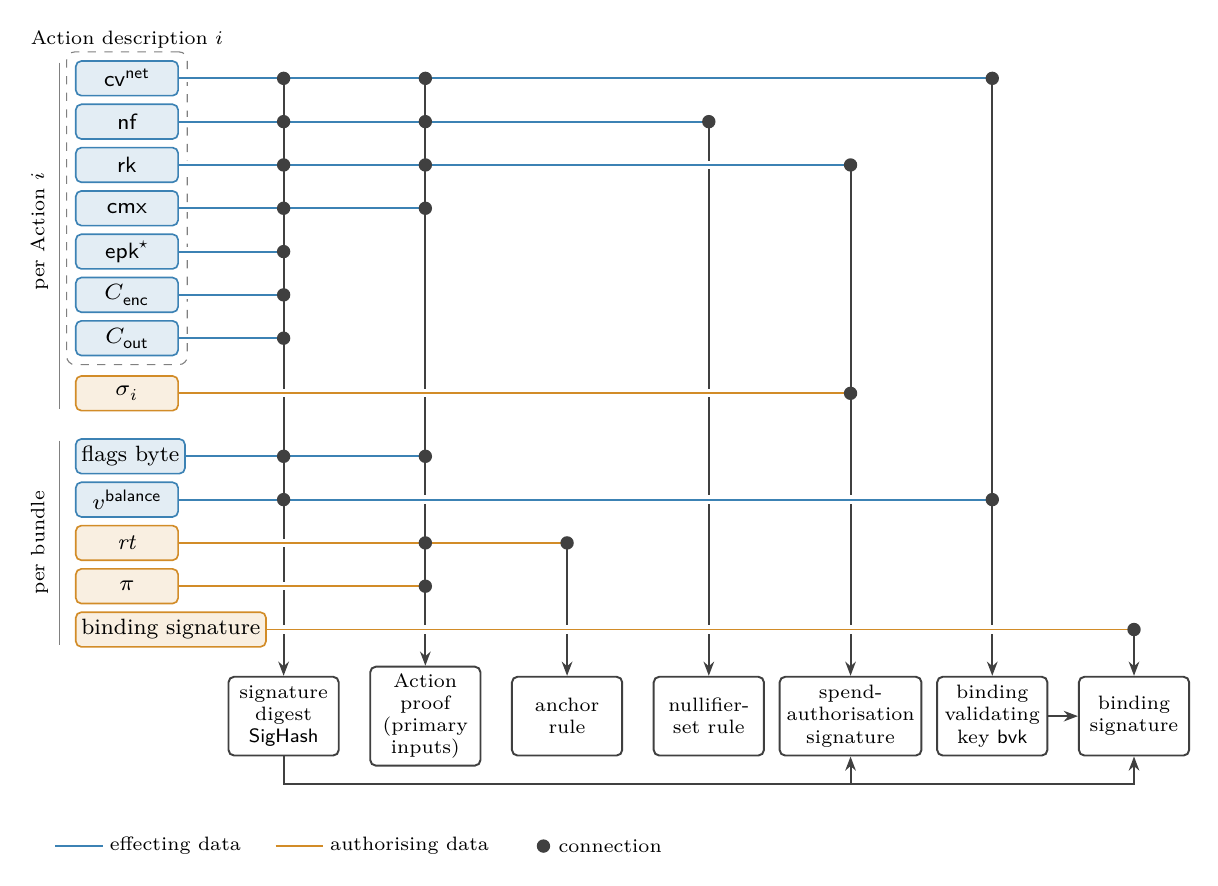
\begin{tikzpicture}[
  font=\footnotesize, >={Stealth[length=1.8mm]},
  fld/.style={draw=#1, fill=#1, fill opacity=0.14, text opacity=1,
    line width=0.6pt, rounded corners=2pt, inner sep=2pt,
    minimum height=4.4mm, minimum width=13mm},
  chk/.style={draw=darkgray, line width=0.7pt, rounded corners=2pt,
    inner sep=2.5pt, align=center, minimum height=10mm,
    minimum width=14mm, font=\scriptsize, fill=white},
  row/.style={line width=0.7pt, draw=#1,
    preaction={draw=white, line width=3pt}},
  bus/.style={->, line width=0.7pt, draw=darkgray},
  jn/.style={circle, fill=darkgray, inner sep=0pt, minimum size=1.7mm},
  lb/.style={font=\scriptsize, inner sep=1pt, align=center},
]
% columns: consumers
\def\ca{2.9}\def\cb{4.7}\def\cc{6.5}\def\cd{8.3}
\def\ce{10.1}\def\cf{11.9}\def\cg{13.7}
\def\ychk{-8.1}
% fields
\foreach \n/\t/\y/\c in {
    cv/{$\cvsym^{\mathsf{net}}$}/0/tierin,
    nf/{$\nfsym$}/-0.55/tierin,
    rk/{$\rk$}/-1.1/tierin,
    cmx/{$\cmx$}/-1.65/tierin,
    epk/{$\mathsf{epk}^{\star}$}/-2.2/tierin,
    ce/{$C_{\mathsf{enc}}$}/-2.75/tierin,
    co/{$C_{\mathsf{out}}$}/-3.3/tierin,
    sg/{$\sigma_i$}/-4.0/tierfull,
    fl/{flags byte}/-4.8/tierin,
    vb/{$v^{\mathsf{balance}}$}/-5.35/tierin,
    rt/{$\mathit{rt}$}/-5.9/tierfull,
    pf/{$\pi$}/-6.45/tierfull,
    bs/{binding signature}/-7.0/tierfull} {
  \node[fld=\c, anchor=west] (\n) at (0.25,\y) {\t};
}
% consumers
\node[chk] (k1) at (\ca,\ychk) {signature\\digest\\$\mathsf{SigHash}$};
\node[chk] (k2) at (\cb,\ychk) {Action\\proof\\(primary\\inputs)};
\node[chk] (k3) at (\cc,\ychk) {anchor\\rule};
\node[chk] (k4) at (\cd,\ychk) {nullifier-\\set rule};
\node[chk] (k5) at (\ce,\ychk) {spend-\\authorisation\\signature};
\node[chk] (k6) at (\cf,\ychk) {binding\\validating\\key $\mathsf{bvk}$};
\node[chk] (k7) at (\cg,\ychk) {binding\\signature};
% buses
\draw[bus] (\ca,0) -- (k1.north);
\draw[bus] (\cb,0) -- (k2.north);
\draw[bus] (\cc,-5.9) -- (k3.north);
\draw[bus] (\cd,-0.55) -- (k4.north);
\draw[bus] (\ce,-1.1) -- (k5.north);
\draw[bus] (\cf,0) -- (k6.north);
\draw[bus] (\cg,-7.0) -- (k7.north);
% rows, each to its rightmost consumer
\foreach \n/\x/\c in {cv/\cf/tierin, nf/\cd/tierin, rk/\ce/tierin,
    cmx/\cb/tierin, epk/\ca/tierin, ce/\ca/tierin, co/\ca/tierin,
    sg/\ce/tierfull, fl/\cb/tierin, vb/\cf/tierin, rt/\cc/tierfull,
    pf/\cb/tierfull, bs/\cg/tierfull} {
  \draw[row=\c] (\n.east) -- (\x,0 |- \n.east);
}
% joins
\foreach \n/\x in {cv/\ca, cv/\cb, cv/\cf, nf/\ca, nf/\cb, nf/\cd,
    rk/\ca, rk/\cb, rk/\ce, cmx/\ca, cmx/\cb, epk/\ca, ce/\ca, co/\ca,
    sg/\ce, fl/\ca, fl/\cb, vb/\ca, vb/\cf, rt/\cb, rt/\cc, pf/\cb,
    bs/\cg} {
  \node[jn] at (\x,0 |- \n.east) {};
}
% digest and bvk to the signatures
\draw[->, line width=0.7pt, darkgray] (k1.south) -- ++(0,-0.35)
  coordinate (bl) -| (k5.south);
\draw[->, line width=0.7pt, darkgray] (bl -| k5.south) -| (k7.south);
\draw[->, line width=0.7pt, darkgray] (k6.east) -- (k7.west);
% groups
\begin{scope}[on background layer]
\node[draw=gray, dashed, rounded corners=3pt, inner sep=3pt,
  fit=(cv) (co)] (box) {};
\end{scope}
\node[lb, anchor=south] at (box.north) {Action description $i$};
\node[lb, rotate=90, anchor=south] at (-0.05,-1.95) {per Action $i$};
\node[lb, rotate=90, anchor=south] at (-0.05,-5.9) {per bundle};
\draw[gray, line width=0.5pt] (0.05,0.2) -- (0.05,-4.2);
\draw[gray, line width=0.5pt] (0.05,-4.6) -- (0.05,-7.2);
% legend
\draw[line width=0.9pt, tierin] (0.0,-9.75) -- (0.6,-9.75);
\node[lb, anchor=west] at (0.65,-9.75) {effecting data};
\draw[line width=0.9pt, tierfull] (2.8,-9.75) -- (3.4,-9.75);
\node[lb, anchor=west] at (3.45,-9.75) {authorising data};
\node[jn] at (6.2,-9.75) {};
\node[lb, anchor=west] at (6.35,-9.75) {connection};
\end{tikzpicture}
\caption{The public data of one bundle and the checks that consume them.
Rows are the fields: per Action~$i$, the net value commitment
$\cvsym^{\mathsf{net}}$, the nullifier $\nfsym$, the randomised validating
key $\rk$, the extracted commitment $\cmx$, the ephemeral key
$\mathsf{epk}^{\star}$ and the ciphertexts $C_{\mathsf{enc}}$ and
$C_{\mathsf{out}}$ of the Action description, and the spend-authorisation
signature $\sigma_i$; per bundle, the flags byte, the balancing value
$v^{\mathsf{balance}}$, the anchor $\mathit{rt}$, the aggregate proof $\pi$
and the binding signature. Each column ends in the check or derived key
that consumes it. A dot joins a field to a column; a row that crosses a
column without a dot is not joined to it. Blue rows are effecting data and
amber rows authorising data (``Transaction digests and signatures'',
\S\ref{sec:tx-sighash}). Every effecting field, the ciphertexts included,
joins the signature digest $\mathsf{SigHash}$, which feeds every
spend-authorisation signature and the binding signature; the anchor and the
proof do not join it (Proposition~\ref{prop:bundle-binding}). The fields
$\nfsym$, $\cmx$, $\cvsym^{\mathsf{net}}$, $\rk$, the flags and
$\mathit{rt}$ are primary inputs of the Action proof; $\mathit{rt}$ also
feeds the anchor rule, $\nfsym$ the nullifier-set rule, $\rk$ the
spend-authorisation signature, and $\cvsym^{\mathsf{net}}$ and
$v^{\mathsf{balance}}$ the binding validating key $\mathsf{bvk}$.}
\label{fig:bundle}
\end{figure}

\FloatBarrier
\subsection{The transaction format}\label{sec:tx-format}

The transaction formats in force are version~$5$, specified in ZIP 225, and
version~$6$, specified in ZIP 229; a transaction of any other version,
version~$4$ included, is invalid (protocol specification, \S``Transaction
Consensus Rules'', as amended by ZIP 2003, ``Specification''; ZIP 259,
Abstract). Of the two Orchard-protocol bundles a version-$5$ transaction can
carry only the Orchard-pool bundle; a transaction with Ironwood-pool Actions
is of version~$6$ (protocol specification, \S``Action Descriptions''). The
Orchard-pool rules of ``Chain state and pool rules'' (\S\ref{sec:tx-pools})
apply to Orchard-pool Actions in both versions (ZIP 229, ``Consensus
Rules''). \emph{Sprout}, Zcash's first shielded protocol, spends its notes
only through \emph{JoinSplit descriptions}, its transfer descriptions, which
only transaction versions $2$ to $4$ carry (protocol specification,
\S``Transaction Encoding and Consensus''); Sprout funds are therefore
unspendable, and their value remains counted as issued, in the sense of the
total issued supply defined in ``Chain state and pool rules''
(\S\ref{sec:tx-pools}) (ZIP 2003, Abstract and ``Interaction with the
proposed Network Sustainability Mechanism''; ZIP 259, Abstract). This
subsection describes version~$6$.

% compute/OUTPUT.md, cited numbers:
% v6 version group 0xD884B698: ZIP 229 'Consensus Rules'
% flagsIronwood bit 2 enableCrossAddress, reserved bits 3..7; flagsOrchard
%   reserved 2..7: ZIP 229 'Consensus Rules'
\begin{construction}[Version-6 transaction]
A version-$6$ transaction consists of the fields of the version-$5$ format
up to and including the Orchard component (ZIP 225), followed by the
Ironwood component. Its first five fields form the header:
\begin{enumerate}[label=(\roman*)]
\item $\mathsf{header}$, whose bit~$31$, the $\mathsf{fOverwintered}$ flag,
  is set and whose bits $0$ to $30$ hold the version, $6$;
\item $\mathsf{nVersionGroupId}$, which must be $\mathtt{0xD884B698}$;
\item $\mathsf{nConsensusBranchId}$, which must equal the consensus branch
  identifier used by the signature digest of ``Transaction digests and
  signatures'' (\S\ref{sec:tx-sighash}), the identifier of the consensus
  branch under which the transaction is validated, where a \emph{consensus
  branch} is a sequence of consecutive blocks under one consensus rule set
  whose first block is the genesis block or follows a block validated under
  older rules, and each network upgrade fixes for the branch that it begins
  a globally unique non-zero $32$-bit \emph{consensus branch identifier}
  (ZIP 200, Terminology and ``Specification'');
\item $\mathsf{lock\_time}$, the transparent lock time, which no rule of
  this volume uses;
\item $\mathsf{nExpiryHeight}$, the \emph{expiry height}.
\end{enumerate}
In version~$6$, bits $0$ and~$1$ of $\mathsf{flagsOrchard}$ are named
$\mathsf{enableSpends}$ and $\mathsf{enableOutputs}$, as in
$\mathsf{flagsIronwood}$, and bits $2$ to~$7$ of $\mathsf{flagsOrchard}$ are
reserved and must be $0$, in version~$5$ and version~$6$ alike (``Bundle
flags'', \S\ref{sec:action-flags}). The Ironwood component has the structure
of the Orchard component, with its own flags, balancing value, anchor, proof
and signatures; both encode each Action as the $820$-byte Action description
of \S\ref{sec:tx-bundle} (ZIP 229, ``Transaction Format'' and ``Consensus
Rules''; protocol specification, \S``Transaction Consensus Rules'').
\end{construction}

\begin{definition}[Coinbase transaction]
A \emph{coinbase transaction} is the first transaction of a block; it
collects the block subsidy, the value newly issued in that block, and the
fees of the block's other transactions. Every block has exactly one
(protocol specification, \S``Coinbase Transactions'').
\end{definition}

% cited constant, not in compute/OUTPUT.md: 499999999, the bound on
%   nExpiryHeight: spec 'Transaction Consensus Rules'; ZIP 203
%   'Specification'
The field $\mathsf{nExpiryHeight}$ is $0$, which disables expiry, or a block
height. The \emph{expiry rule} is: for a transaction other than a coinbase
transaction, $\mathsf{nExpiryHeight}$ is at most $499\,999\,999$, and such a
transaction with $\mathsf{nExpiryHeight} \neq 0$ is invalid in every block
of height greater than $\mathsf{nExpiryHeight}$; the
$\mathsf{nExpiryHeight}$ of a coinbase transaction equals the height of its
block (protocol specification, \S``Transaction Consensus Rules''; ZIP 203,
``Specification''; ZIP 229, ``Transaction Format''). The sender's choice of
the expiry height is stated in ``Construction of a transaction''
(\S\ref{sec:tx-construct}).

% compute/encodings.py:
% [sec:tx-format] Action description = 5 x 32 (cv_net, nf, rk, cmx, epk)
%   + 580 + 80 = 820 bytes
% [sec:tx-format] proof = 2720 + 2272 n bytes (consensus rule); n = 1: 4992,
%   n = 2: 7264
% [sec:tx-format] check only: 2720 = 85 x 32 and 2272 = 71 x 32 (32-byte
%   elements); IPA share = 23 points + 2 scalars = 800 bytes of the 2720;
%   the Halo 2 Guide derives no other part of either constant
% compute/OUTPUT.md, cited numbers:
% 820 bytes per Action; flags 1, balancing value 8, anchor 32, signatures
%   64 bytes; proof 2720 + 2272 n: ZIP 229 'Transaction Format'
% fewer than 2^16 Ironwood Actions: ZIP 229 'Consensus Rules'
% MAX_MONEY = 2.1 x 10^15 zatoshi: spec 'Constants'
% valueBalanceIronwood in [-MAX_MONEY, MAX_MONEY]: spec 'Transaction
%   Consensus Rules'
\begin{definition}[Ironwood component]
Let $n$ be the number of Ironwood-pool Actions of a version-$6$
transaction. The \emph{Ironwood component} is the sequence of the fields of
Table~\ref{tab:tx-ironwood}, in that order. The fields after
$\mathsf{nActionsIronwood}$ are present if and only if $n > 0$, and an
absent $\mathsf{valueBalanceIronwood}$ is taken to be $0$. A count and a
proof length are encoded as \emph{compactSize}, the variable-length integer
encoding of Bitcoin (ZIP 229, ``Transaction Format'').
\end{definition}

\begin{table}[tp]
\centering\small
\setlength{\tabcolsep}{5pt}
\begin{tabular}{@{}llp{7.4cm}@{}}
\toprule
Field & Bytes & Content \tabularnewline
\midrule
$\mathsf{nActionsIronwood}$ & compactSize
  & \raggedright the count $n$ \tabularnewline
$\mathsf{vActionsIronwood}$ & $820\,n$
  & \raggedright the $n$ Action descriptions of \S\ref{sec:tx-bundle}
  \tabularnewline
$\mathsf{flagsIronwood}$ & $1$
  & \raggedright bit~$0$ $\mathsf{enableSpends}$, bit~$1$
  $\mathsf{enableOutputs}$, bit~$2$ $\mathsf{enableCrossAddress}$, bits
  $3$ to~$7$ reserved and $0$ \tabularnewline
$\mathsf{valueBalanceIronwood}$ & $8$
  & \raggedright the balancing value, signed $64$-bit little-endian
  \tabularnewline
$\mathsf{anchorIronwood}$ & $32$
  & \raggedright the anchor $\mathit{rt}$ \tabularnewline
$\mathsf{sizeProofsIronwood}$ & compactSize
  & \raggedright the proof length, $2720 + 2272\,n$ \tabularnewline
$\mathsf{proofsIronwood}$ & $2720 + 2272\,n$
  & \raggedright the aggregate proof \tabularnewline
$\mathsf{vSpendAuthSigsIronwood}$ & $64\,n$
  & \raggedright one spend-authorisation signature per Action, in Action
  order \tabularnewline
$\mathsf{bindingSigIronwood}$ & $64$
  & \raggedright the binding signature \tabularnewline
\bottomrule
\end{tabular}
\caption{The Ironwood component of a version-$6$ transaction with $n$
Ironwood-pool Actions (ZIP 229, ``Transaction Format''). The fields after
the count are present if and only if $n > 0$.}
\label{tab:tx-ironwood}
\end{table}

The consensus rules on the component are: $n < 2^{16}$; if $n > 0$, at least
one of $\mathsf{enableSpends}$ and $\mathsf{enableOutputs}$ of
$\mathsf{flagsIronwood}$ is $1$; bits $3$ to~$7$ of $\mathsf{flagsIronwood}$
are $0$; $\mathsf{valueBalanceIronwood}$ lies in
$\{-\mathsf{MAX\_MONEY}, \dots, \mathsf{MAX\_MONEY}\}$, where
$\mathsf{MAX\_MONEY} = 2.1 \cdot 10^{15}$ zatoshi is a protocol constant
(protocol specification, \S``Constants''); and $\mathsf{proofsIronwood}$
has exactly $2720 + 2272\,n$ bytes (ZIP 229, ``Consensus Rules''; protocol
specification, \S``Transaction Consensus Rules'' and \S``Action Description
Encoding and Consensus''). The flags byte differs from $\mathsf{flagsOrchard}$
only in bit~$2$, which is $\mathsf{enableCrossAddress}$ in
$\mathsf{flagsIronwood}$ and reserved and $0$ in $\mathsf{flagsOrchard}$
(``Bundle flags'', \S\ref{sec:action-flags}). The proof length is the one
that ZIP 229 fixes; the \emph{Halo 2 Guide}, \S``The complete Halo 2
protocol'', paragraph ``Proof size'', describes what its constant and its
per-Action term cover. For one Action the proof has
$2720 + 2272 = 4992$ bytes.

\FloatBarrier
\subsection{Transaction digests and signatures}\label{sec:tx-sighash}

Write $\mathsf{h}(P, x) := \mathrm{BLAKE2b\text{-}256}(P, x)$, unkeyed
BLAKE2b with a $32$-byte output, the $16$-byte personalisation $P$ and the
input $x$ (\S\ref{sec:enc-encrypt}); the personalisation is mixed into the
initialisation vector (\emph{Crypto Guide}, \S``Domain separation and
personalisation''). For a byte string $C$ and $0 \le a \le b \le |C|$, the
string $C[a{:}b]$ consists of the bytes $a$ to $b - 1$ of $C$, counted from
$0$. Every field enters a digest in its encoding of
Table~\ref{tab:tx-action} or Table~\ref{tab:tx-ironwood}, and $\beta$
denotes the $4$-byte little-endian encoding of the consensus branch
identifier.

\begin{definition}[Transaction identifier]
The \emph{transaction identifier} of a version-$6$ transaction is
\[
  \mathsf{txid} := \mathsf{h}\bigl(\texttt{ZcashTxHash\_} \,\|\, \beta,\
    d_{\mathsf{hdr}} \,\|\, d_{\mathsf{tr}} \,\|\, d_{\mathsf{Sap}}
    \,\|\, d_{\mathsf{Orc}} \,\|\, d_{\mathsf{Irw}}\bigr),
\]
the Ironwood digest last, where:
\begin{enumerate}[label=(\roman*)]
\item the \emph{header digest} $d_{\mathsf{hdr}}$ is $\mathsf{h}$ under
  $\texttt{ZTxIdHeadersHash}$ of the $4$-byte little-endian encodings of
  $\mathsf{header}$, $\mathsf{nVersionGroupId}$,
  $\mathsf{nConsensusBranchId}$, $\mathsf{lock\_time}$ and
  $\mathsf{nExpiryHeight}$;
\item the \emph{transparent digest} $d_{\mathsf{tr}}$ and the \emph{Sapling
  digest} $d_{\mathsf{Sap}}$ are those of ZIP 244, ``T.2:
  transparent\_digest'' and ``T.3: sapling\_digest'', the latter with the
  version-$6$ node of ZIP 229; they cover the transparent inputs and
  outputs and the Sapling component, the component of Zcash's second
  shielded protocol;
\item for $n \ge 1$ Ironwood-pool Actions, with the fields of Action~$i$
  indexed by $i$, the \emph{Ironwood digest} is
  \begin{align*}
    d_{\mathsf{Irw}} &:= \mathsf{h}\bigl(\texttt{ZTxIdIronwd\_H\_v6},\
      d_{\mathsf{C}} \,\|\, d_{\mathsf{M}} \,\|\, d_{\mathsf{N}} \,\|\,
      \mathsf{flagsIronwood} \,\|\, \mathsf{valueBalanceIronwood}\bigr),
      \\
    d_{\mathsf{X}} &:= \mathsf{h}\bigl(P_{\mathsf{X}},\
      r^{\mathsf{X}}_1 \,\|\, \cdots \,\|\, r^{\mathsf{X}}_n\bigr)
      \qquad (\mathsf{X} \in \{\mathsf{C}, \mathsf{M}, \mathsf{N}\}),
  \end{align*}
  with the \emph{compact}, \emph{memo} and \emph{non-compact} records and
  personalisations
  \begin{align*}
    r^{\mathsf{C}}_i &:= \nfsym_i \,\|\, \cmx_i \,\|\,
      \mathsf{epk}_i^{\star} \,\|\, C_{\mathsf{enc},i}[0{:}52], &
    P_{\mathsf{C}} &:= \texttt{ZTxIdIrnActCH\_v6}, \\
    r^{\mathsf{M}}_i &:= C_{\mathsf{enc},i}[52{:}564], &
    P_{\mathsf{M}} &:= \texttt{ZTxIdIrnActMH\_v6}, \\
    r^{\mathsf{N}}_i &:= (\cvsym^{\mathsf{net}}_i)^{\star} \,\|\,
      \rk_i^{\star} \,\|\, C_{\mathsf{enc},i}[564{:}580] \,\|\,
      C_{\mathsf{out},i}, &
    P_{\mathsf{N}} &:= \texttt{ZTxIdIrnActNH\_v6};
  \end{align*}
  for $n = 0$ it is
  $d_{\mathsf{Irw}} := \mathsf{h}(\texttt{ZTxIdIronwd\_H\_v6},
  \varepsilon)$;
\item the \emph{Orchard digest} $d_{\mathsf{Orc}}$ has the same structure
  over the Orchard-pool Actions, with $\mathsf{flagsOrchard}$ and
  $\mathsf{valueBalanceOrchard}$, under the personalisation
  $\texttt{ZTxIdOrchardH\_v6}$, with the Action digests personalised
  \[
    P_{\mathsf{C}} = \texttt{ZTxIdOrcActCHash}, \quad
    P_{\mathsf{M}} = \texttt{ZTxIdOrcActMHash}, \quad
    P_{\mathsf{N}} = \texttt{ZTxIdOrcActNHash};
  \]
  without Orchard-pool Actions it is
  $\mathsf{h}(\texttt{ZTxIdOrchardH\_v6}, \varepsilon)$.
\end{enumerate}
(ZIP 244, ``Digests'', ``txid\_digest'', ``T.1: header\_digest'' and ``T.4:
orchard\_digest''; ZIP 229, ``Ironwood component digest'', ``Anchor
commitment (version 6)'' and ``Summary of the resulting digest
structure''.)
\end{definition}

% compute/encodings.py:
% [sec:tx-sighash] C_enc[..52] compact (lead byte, d, v, rseed),
%   C_enc[52..564] memo, C_enc[564..] the 16-byte tag
% [sec:enc-plaintext] note plaintext = 1 (lead byte) + 11 (d) + 8 (v)
%   + 32 (rseed) + 512 (memo) = 564 bytes
% [sec:enc-encrypt] C_enc = 564 + 16 (AEAD tag) = 580 bytes
The ciphertext $C_{\mathsf{enc}}$ is the ChaCha20 encryption of the
$564$-byte note plaintext, byte for byte, followed by the $16$-byte tag
(\emph{Crypto Guide}, \S``The ChaCha20-Poly1305 AEAD'', Construction
``ChaCha20-Poly1305''; ``The note plaintext'', \S\ref{sec:enc-plaintext}).
The offsets therefore split it into the encryption of the $52$-byte prefix
of the plaintext, the lead byte, $d$, $v$ and $\mathsf{rseed}$
($1 + 11 + 8 + 32 = 52$), the encryption of the $512$-byte memo, ending at
$52 + 512 = 564$, and the tag. The empty Ironwood digest differs from the
empty Orchard digest, since the two personalisations differ. Neither pool
digest contains the anchor.

\begin{definition}[Authorising-data digest; effecting and authorising data]
The \emph{authorising-data digest} of a version-$6$ transaction is
\[
  \mathsf{auth} := \mathsf{h}\bigl(\texttt{ZTxAuthHash\_} \,\|\, \beta,\
    a_{\mathsf{tr}} \,\|\, a_{\mathsf{Sap}} \,\|\, a_{\mathsf{Orc}}
    \,\|\, a_{\mathsf{Irw}}\bigr),
\]
where $a_{\mathsf{tr}}$ is the transparent scripts digest and
$a_{\mathsf{Sap}}$ the Sapling authorising-data digest (ZIP 244,
``Authorizing Data Commitment''; ZIP 229), and, for $n \ge 1$
Ironwood-pool Actions,
\begin{align*}
  a_{\mathsf{Irw}} := \mathsf{h}\bigl(\texttt{ZTxAuthIrnwdH\_v6},\
    &\mathsf{proofsIronwood} \,\|\, \mathsf{vSpendAuthSigsIronwood} \\
    &\,\|\, \mathsf{bindingSigIronwood} \,\|\, \mathsf{anchorIronwood}
    \bigr),
\end{align*}
and $a_{\mathsf{Irw}} := \mathsf{h}(\texttt{ZTxAuthIrnwdH\_v6},
\varepsilon)$ for $n = 0$; the Orchard digest $a_{\mathsf{Orc}}$ has the
same structure under $\texttt{ZTxAuthOrchaH\_v6}$. Each Orchard-protocol
anchor is committed if and only if its component has Actions. The
\emph{effecting data} of a transaction are the data under the transaction
identifier digest; its \emph{authorising data} are the proofs, the
signatures, the anchors and the transparent scripts, the data under the
authorising-data digest (ZIP 229, ``Ironwood component digest'' and
``Anchor commitment (version 6)''; ZIP 244, ``Authorizing Data
Commitment'').
\end{definition}

ZIP 244, ``Authorizing Data Commitment'', describes the pair of the
transaction identifier and the authorising-data digest as a commitment to
all data of the transaction. In version~$6$ the anchors are authorising
data so that a transaction can be signed before its anchor is chosen and its
proofs are computed; replacing a bundle's anchor and proof together does not
change the transaction identifier (ZIP 229, Motivation and ``Anchor
commitment (version 6)''). Below the two roots, a node whose directly
hashed input differs between versions $5$ and~$6$ has a version-$6$
personalisation of its own; the roots keep theirs and hash one more child in
version~$6$. The nodes that omit or include an anchor in version~$6$ are
personalised $\texttt{ZTxIdSSpendNH\_v6}$, $\texttt{ZTxAuthSapliH\_v6}$,
$\texttt{ZTxIdOrchardH\_v6}$ and $\texttt{ZTxAuthOrchaH\_v6}$ (ZIP 229,
``Ironwood component digest'' and ``Anchor commitment (version 6)'').

\begin{definition}[Signature digest]
The \emph{signature digest} of a transaction is its digest not associated
with a transparent input, under the hash type $\mathsf{SIGHASH\_ALL}$,
which covers all transparent inputs and outputs:
\[
  \mathsf{SigHash} := \mathsf{h}\bigl(\texttt{ZcashTxHash\_} \,\|\, \beta,\
    d_{\mathsf{hdr}} \,\|\, s_{\mathsf{tr}} \,\|\, d_{\mathsf{Sap}}
    \,\|\, d_{\mathsf{Orc}} \,\|\, d_{\mathsf{Irw}}\bigr),
\]
whose header and shielded children are those of $\mathsf{txid}$ and whose
child $s_{\mathsf{tr}}$ is the transparent signature digest of ZIP 244,
``S.2: transparent\_sig\_digest''. For a coinbase transaction and for a
transaction without transparent inputs, $s_{\mathsf{tr}} = d_{\mathsf{tr}}$,
so $\mathsf{SigHash} = \mathsf{txid}$; otherwise $s_{\mathsf{tr}}$ commits in
addition to the values and scripts of the coins that the transparent inputs
spend. The digest $\mathsf{SigHash}$ is the message of every
spend-authorisation signature and of each pool's binding signature, the
message left as a parameter in ``The RedPallas signature scheme''
(\S\ref{sec:spendauth-redpallas}) (ZIP 244, ``Signature Digest''; ZIP 229,
``Transaction Identifiers, Auth Digests, and Signature Digests''; protocol
specification, \S``Action Descriptions'' and \S``Balance and Binding
Signature (Orchard)'').
\end{definition}

Proposition~\ref{prop:bvk}, which holds for every message, applies to the
binding signature on $\mathsf{SigHash}$.

\begin{remark}[Version 5]
In version~$5$ the root of the transaction identifier has four children,
the header, transparent, Sapling and Orchard digests, under the same root
personalisation. The Orchard digest, under $\texttt{ZTxIdOrchardHash}$,
hashes
\[
  d_{\mathsf{C}} \,\|\, d_{\mathsf{M}} \,\|\, d_{\mathsf{N}} \,\|\,
  \mathsf{flagsOrchard} \,\|\, \mathsf{valueBalanceOrchard} \,\|\,
  \mathsf{anchorOrchard},
\]
with the Action digests of version~$6$, and the
Orchard authorising-data digest, under $\texttt{ZTxAuthOrchaHash}$, covers
the proofs and the signatures only. In version~$5$ the Orchard anchor is
therefore effecting data and fixed by the signatures; the proofs are
authorising data in both versions. A version-$5$ transaction carries
Orchard-pool Actions only (ZIP 244, ``txid\_digest'', ``T.4:
orchard\_digest'' and ``A.3: orchard\_auth\_digest'').
\end{remark}

\begin{figure}[tp]
\centering
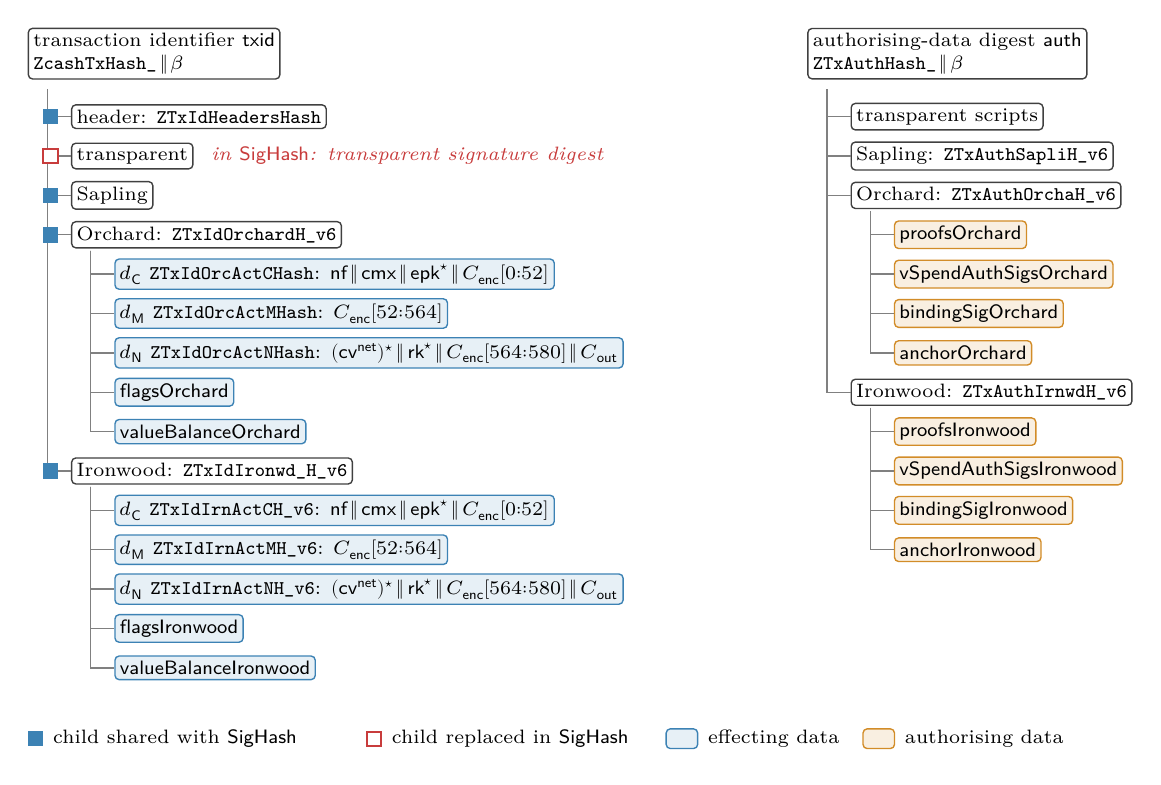
\begin{tikzpicture}[
  font=\scriptsize,
  dg/.style={anchor=west, draw=darkgray, line width=0.5pt,
    rounded corners=1.5pt, inner sep=1.8pt, fill=white, align=left},
  ef/.style={anchor=west, draw=tierin, line width=0.5pt,
    rounded corners=1.5pt, inner sep=1.8pt, fill=tierin,
    fill opacity=0.12, text opacity=1},
  au/.style={anchor=west, draw=tierfull, line width=0.5pt,
    rounded corners=1.5pt, inner sep=1.8pt, fill=tierfull,
    fill opacity=0.14, text opacity=1},
  tr/.style={line width=0.5pt, draw=gray},
  sh/.style={draw=tierin, fill=tierin, line width=0.5pt,
    minimum size=1.8mm, inner sep=0pt},
  nsh/.style={draw=tierspend, fill=white, line width=0.7pt,
    minimum size=1.8mm, inner sep=0pt},
]
% transaction identifier
\node[dg] (T) at (0,0) {transaction identifier $\mathsf{txid}$\\
  $\texttt{ZcashTxHash\_} \,\|\, \beta$};
\foreach \n/\t/\y in {
    th/{header: $\texttt{ZTxIdHeadersHash}$}/-0.8,
    tt/{transparent}/-1.3,
    ts/{Sapling}/-1.8,
    to/{Orchard: $\texttt{ZTxIdOrchardH\_v6}$}/-2.3,
    ti/{Ironwood: $\texttt{ZTxIdIronwd\_H\_v6}$}/-5.3} {
  \node[dg] (\n) at (0.55,\y) {\t};
  \draw[tr] (0.25,-0.45) |- (\n.west);
}
\foreach \pp/\pa/\pb/\pc/\y in {o/OrcActCHash/OrcActMHash/OrcActNHash/-2.3,
    i/IrnActCH\_v6/IrnActMH\_v6/IrnActNH\_v6/-5.3} {
  \node[ef] (\pp c) at (1.1,{\y-0.5}) {$d_{\mathsf{C}}$
    $\texttt{ZTxId\pa}$: $\nfsym \,\|\, \cmx \,\|\, \mathsf{epk}^{\star}
    \,\|\, C_{\mathsf{enc}}[0{:}52]$};
  \node[ef] (\pp m) at (1.1,{\y-1.0}) {$d_{\mathsf{M}}$
    $\texttt{ZTxId\pb}$: $C_{\mathsf{enc}}[52{:}564]$};
  \node[ef] (\pp n) at (1.1,{\y-1.5}) {$d_{\mathsf{N}}$
    $\texttt{ZTxId\pc}$: $(\cvsym^{\mathsf{net}})^{\star} \,\|\,
    \rk^{\star} \,\|\, C_{\mathsf{enc}}[564{:}580] \,\|\,
    C_{\mathsf{out}}$};
  \foreach \kk in {c, m, n} {
    \draw[tr] (0.8,{\y-0.2}) |- (\pp\kk.west);
  }
}
\node[ef] (of) at (1.1,-4.3) {$\mathsf{flagsOrchard}$};
\node[ef] (ov) at (1.1,-4.8) {$\mathsf{valueBalanceOrchard}$};
\node[ef] (if) at (1.1,-7.3) {$\mathsf{flagsIronwood}$};
\node[ef] (iv) at (1.1,-7.8) {$\mathsf{valueBalanceIronwood}$};
\foreach \kk/\y in {of/-2.3, ov/-2.3, if/-5.3, iv/-5.3} {
  \draw[tr] (0.8,{\y-0.2}) |- (\kk.west);
}
% markers: children shared with SigHash
\foreach \n in {th, ts, to, ti} {
  \node[sh] at ([xshift=-2.6mm]\n.west) {};
}
\node[nsh] at ([xshift=-2.6mm]tt.west) {};
\node[anchor=west, text=tierspend, font=\scriptsize\itshape]
  at ([xshift=1mm]tt.east)
  {in $\mathsf{SigHash}$: transparent signature digest};
% authorising-data digest
\node[dg] (A) at (9.9,0) {authorising-data digest $\mathsf{auth}$\\
  $\texttt{ZTxAuthHash\_} \,\|\, \beta$};
\foreach \n/\t/\y in {
    at/{transparent scripts}/-0.8,
    as/{Sapling: $\texttt{ZTxAuthSapliH\_v6}$}/-1.3,
    ao/{Orchard: $\texttt{ZTxAuthOrchaH\_v6}$}/-1.8,
    ai/{Ironwood: $\texttt{ZTxAuthIrnwdH\_v6}$}/-4.3} {
  \node[dg] (\n) at (10.45,\y) {\t};
  \draw[tr] (10.15,-0.45) |- (\n.west);
}
\foreach \pp/\pn/\y in {o/Orchard/-1.8, i/Ironwood/-4.3} {
  \foreach \ff/\kk in {proofs/1, vSpendAuthSigs/2, bindingSig/3,
      anchor/4} {
    \node[au] (\pp\ff) at (11.0,{\y-0.5*\kk}) {$\mathsf{\ff\pn}$};
    \draw[tr] (10.7,{\y-0.2}) |- (\pp\ff.west);
  }
}
% legend
\node[sh] (l1) at (0.1,-8.7) {};
\node[anchor=west] at (l1.east) {child shared with
  $\mathsf{SigHash}$};
\node[nsh] (l2) at (4.4,-8.7) {};
\node[anchor=west] at (l2.east) {child replaced in $\mathsf{SigHash}$};
\node[ef, minimum width=4mm, minimum height=2.5mm] (l3) at (8.1,-8.7) {};
\node[anchor=west] at (l3.east) {effecting data};
\node[au, minimum width=4mm, minimum height=2.5mm] (l4) at (10.6,-8.7) {};
\node[anchor=west] at (l4.east) {authorising data};
\end{tikzpicture}
\caption{The version-$6$ transaction identifier (left) and authorising-data
digest (right) as trees of personalised BLAKE2b-256 nodes, with the Orchard
and Ironwood components expanded (ZIP 244; ZIP 229). Each node hashes the
concatenation of its children, in order, under the personalisation shown;
the string $\beta$ encodes the consensus branch identifier. The Action digests
$d_{\mathsf{C}}$, $d_{\mathsf{M}}$ and $d_{\mathsf{N}}$ hash the listed
fields of every Action of their component, Action after Action; the byte
$\mathsf{flagsIronwood}$ is the Ironwood component's own flags byte. The
header, transparent and Sapling digests are not expanded. The signature
digest $\mathsf{SigHash}$ has the root personalisation and the children of
$\mathsf{txid}$ (filled squares), except the transparent child (open
square), which it replaces by the transparent signature digest. The anchors
and the proofs lie under the authorising-data digest only. By
Proposition~\ref{prop:bundle-binding}, the signatures fix every field under
$\mathsf{txid}$ and no field under the authorising-data digest.}
\label{fig:sighash}
\end{figure}

Figure~\ref{fig:sighash} draws both trees. The binding of the signatures
needs one further assumption, stated at its first use.

\begin{assumption}[Collision resistance of BLAKE2b]\label{ass:blake2b-cr}
No efficient algorithm outputs, except with negligible probability, two
distinct pairs $(P, x)$ and $(P', x')$, each of a $16$-byte personalisation
and an input string, with $\mathsf{h}(P, x) = \mathsf{h}(P', x')$. The notion
is the \emph{Crypto Guide}'s Definition ``Collision resistance''
(\S``Security notions: preimage, second-preimage, and collision
resistance''), read for the unkeyed deployment as that volume's Remark
``Convention: keyed definitions, unkeyed deployments'' (\S``Hash functions
and the random oracle model'', \S``Syntax'') prescribes; the
personalisation is mixed into the initialisation vector (\S``Domain
separation and personalisation''), so the pair $(P, x)$ is the hashed input.
It is used by Proposition~\ref{prop:bundle-binding} and by the
consensus-branch binding below.
\end{assumption}

\begin{proposition}[Bundle binding]\label{prop:bundle-binding}
Let $T$ be a version-$6$ transaction, and for a bundle of $T$, of either
pool, let $\rk_1, \dots, \rk_n$ be the randomised validating keys of its
Actions, $\rk_i = [\rsk_i]\,G^{\mathsf{SpendAuth}}$ with
$\rsk_i = \ask_i + \alpha_i$ as in ``Randomised validating keys''
(\S\ref{sec:spendauth-rk}), where $\ask_i$ is the spend authorising key of
the spending key that authorises Action~$i$. Assume:
\begin{enumerate}
\item[(H)] each $\ask_i$ is uniform on the non-zero scalars $a$ for which
  $[a]\,G^{\mathsf{SpendAuth}}$ has even $y$-coordinate (\S\ref{sec:keys-sk}),
  and every value of the experiment other than a signature by the holder of
  $\ask_i$ is computed from $\aksym^{\PP}_i = [\ask_i]\,G^{\mathsf{SpendAuth}}$
  and from values drawn independently of $\ask_i$;
\item[(S)] the holder of $\ask_i$ signs under $\rsk_i$ only
  $\mathsf{SigHash}(T)$, and signs any other message only under
  $\ask_i + \alpha$ for a fresh randomiser $\alpha$ drawn by
  $\mathsf{GenRandom}$.
\end{enumerate}
An adversary receives $T$ and all other public data, and obtains on request,
for messages of its choice, signatures of the key holders under fresh
randomisers as in~(S); it receives no $\ask_i$ and no $\rsk_i$. Under
Assumptions~\ref{ass:blake2b-cr}, \ref{ass:dl-pallas}
and~\ref{ass:hstar-ro}, the probability that it outputs an accepted
transaction $T'$ that contains an Action description with validating key
$\rk_i$ for some $i$ and whose effecting data differ from those of $T$ is
negligible.

The signatures thus fix the effecting data: every Action's $\nfsym$,
$\cmx$, $\cvsym^{\mathsf{net}}$, $\rk$, $\mathsf{epk}$, $C_{\mathsf{enc}}$
and $C_{\mathsf{out}}$, the number and order of the Actions, each bundle's
flags and balancing value, the header, with the consensus branch identifier
and the expiry height, and the transparent data. They fix neither the anchor
nor the proof of a bundle: for a pair $(\mathit{rt}', \pi')$ such that
$\pi'$ verifies on the primary inputs formed with $\mathit{rt}'$, replacing
$(\mathit{rt}, \pi)$ by $(\mathit{rt}', \pi')$ changes neither the
transaction identifier nor any signed message, so every signature remains
valid, and $\pi'$ binds $\mathit{rt}'$ as a primary input
(Definition~\ref{def:action}).
\end{proposition}

\begin{proof}
Let $E$ be the event that the adversary outputs such a $T'$. On $E$, let
$i$ be the least index for which $T'$ contains an Action description with
key $\rk_i$, and let $\sigma'$ be the spend-authorisation signature that
$T'$ carries for it. Since $T'$ is accepted, $\sigma'$ is valid under
$\rk_i$ on $m' := \mathsf{SigHash}(T')$ (``Randomised validating keys'',
\S\ref{sec:spendauth-rk}). Let $m := \mathsf{SigHash}(T)$, and split $E$
into $E_{=}$, where $m' = m$, and $E_{\neq}$, where $m' \neq m$.

\emph{Case $E_{=}$: a collision.} The digest $\mathsf{SigHash}$ is computed
by the tree of its definition from the effecting data and, when the
transaction has transparent inputs, from the values and scripts of the coins
that they spend. Each node hashes a string from which its children and its
fields are recovered uniquely: its input consists of fixed-length fields and
digests, of concatenations of fixed-length per-Action records whose number
the length determines, or, for transparent outputs, of records whose
variable-length script carries its length; the two nodes that share a
personalisation, the transparent digest and the transparent signature
digest, hash strings of different lengths (ZIP 244, ``TxId Digest'' and
``Signature Digest''). Compare the trees of $T$ and $T'$ from the root,
whose outputs are equal. At a node with equal outputs, either the two
(personalisation, input) pairs differ, a collision of $\mathsf{h}$, or they
agree, and then the node's children have equal outputs and its fields are
equal. The effecting data of $T$ and $T'$ differ, so some field, or some
number of records, differs, and descending along the nodes that cover it
ends in a collision. An algorithm that runs the experiment, which it can
since it samples every key, and performs this descent outputs a collision
with probability $\Pr[E_{=}]$, which is negligible by
Assumption~\ref{ass:blake2b-cr}.

\emph{Case $E_{\neq}$: a forgery.} An algorithm $\mathcal{B}$ plays the
adversary of Proposition~\ref{prop:redpallas-euf}. It receives
$Y = [x]\,G^{\mathsf{SpendAuth}}$ for $x$ uniform on $\F_{p_{\Vesta}}$, with
access to $\mathsf{H}$ and to the signing oracle, and draws $i^{*}$
uniformly from $\{1, \dots, n\}$. If $Y = \mathcal{O}$ or $Y$ has odd
$y$-coordinate, it stops; otherwise, an event of probability
$(p_{\Vesta} - 1)/(2 p_{\Vesta})$, the point $Y$ has the distribution that
(H) gives to $\aksym^{\PP}_{i^{*}}$, and $\mathcal{B}$ sets
$\aksym^{\PP}_{i^{*}} := Y$. It computes every other value of the
experiment as (H) permits, in particular the proof of $T$, whose witness
(Definition~\ref{def:action}) contains $\aksym^{\PP}$ and $\alpha$ but not
$\ask$; it draws every randomiser by $\mathsf{GenRandom}$ itself; it
obtains each signature by the holder of $\ask_{i^{*}}$, on $m$ and on the
adversary's requests, as the oracle's answer on the pair $(\alpha, M)$; and
it produces the other signatures with keys it holds. The adversary's view is
then that of the experiment. On $E_{\neq}$ with $i = i^{*}$, $\mathcal{B}$
outputs $(\rk_{i^{*}}, m', \sigma')$ with the randomiser $\alpha_{i^{*}}$,
of its own choice, as part~(ii) of Proposition~\ref{prop:redpallas-euf}
admits. The oracle answered under the key $\rk_{i^{*}}$ only on $m$, except
when a randomiser drawn for a request equals $\alpha_{i^{*}}$, which has
negligible probability by the lemma on the distance of $\mathsf{GenRandom}$
from uniform (\S\ref{sec:spendauth-rk}); outside that event the output is a
forgery. The index $i^{*}$ is independent of the adversary's view, so
$\mathcal{B}$ forges with probability at least
\[
  \frac{p_{\Vesta} - 1}{2 p_{\Vesta}} \cdot \frac{\Pr[E_{\neq}]}{n}
\]
less a negligible term, where $n < 2^{16}$. By
Proposition~\ref{prop:redpallas-euf}(ii), under
Assumptions~\ref{ass:dl-pallas} and~\ref{ass:hstar-ro}, $\Pr[E_{\neq}]$ is
negligible.

\emph{Anchor and proof.} By the definitions above, the anchor and the proof
of each bundle are inputs of the authorising-data digest and of no node of
$\mathsf{txid}$ or $\mathsf{SigHash}$. Replacing them changes neither, and
every signature, whose message is $\mathsf{SigHash}$, remains valid. The
verifier checks the bundle's proof against the primary inputs formed with
the bundle's anchor field (protocol specification, \S``Action
Descriptions''), now $\mathit{rt}'$, so the modified bundle is accepted only
if $\pi'$ verifies for $\mathit{rt}'$, and the anchor rule then applies to
$\mathit{rt}'$.
\end{proof}

\begin{remark}[Hypothesis (H) for honest keys]
For keys generated with $\mathsf{use\_qsk} = \mathsf{false}$ from uniform
spending keys, hypothesis~(H) holds up to a negligible change in the
probability of every efficiently decidable event, in particular of the event
of Proposition~\ref{prop:bundle-binding}, which an algorithm holding the
keys decides by verifying $T'$ and comparing its effecting data with those
of $T$. By Lemma~\ref{lem:prf-independence} (Assumption~\ref{ass:prf-expand})
the triple $(\ask, \nksym, \rivk)$ is indistinguishable from independent uniform
elements; the sign normalisation of ``The spending key and the spend-side
secrets'' (\S\ref{sec:keys-sk}) maps a uniform non-zero $\ask$ to the
uniform distribution on the set of~(H); and rejection, by Lemma ``Rejection
in key generation'' (\S\ref{sec:keys-viewing}), costs a negligible term under
Assumptions~\ref{ass:prf-expand}, \ref{ass:dl-pallas}
and~\ref{ass:grouphash-ro}. A dummy spend uses such a key (Definition
``Dummy notes'', \S\ref{sec:notes-action}).
\end{remark}

\begin{remark}[Consensus-branch binding]
The consensus branch identifier enters $\mathsf{SigHash}$ twice, in the root
personalisation and in the header digest, and a consensus rule requires
$\mathsf{nConsensusBranchId}$ to equal the identifier of the consensus branch
under which the transaction is validated (protocol specification,
\S``Transaction Consensus Rules''; ZIP 244, ``txid\_digest'' and ``T.1:
header\_digest''). Under any other branch a signed transaction $T$ either
fails that rule or carries another $\mathsf{nConsensusBranchId}$, hence other
effecting data, and Proposition~\ref{prop:bundle-binding} excludes valid
signatures on such a transaction that keeps an Action of $T$, except with
negligible probability. A signed transaction is therefore valid under one
consensus branch only and cannot be carried across the activation of a
network upgrade (ZIP 259, ``Backward compatibility''). That the anchors and
the proofs are authorising data does not affect this binding, since the
header is effecting data.
\end{remark}

\FloatBarrier
\subsection{Chain state and pool rules}\label{sec:tx-pools}

The Orchard pool and the Ironwood pool each have their own chain state: a
note commitment tree (``The Merkle hash and the tree'',
\S\ref{sec:tree-hash}) with its anchors (``Anchors'',
\S\ref{sec:tree-anchors}), a nullifier set (``Nullifier sets'',
\S\ref{sec:nf-sets}) and a chain value pool balance, defined below. An
Action is checked only against the state of its own pool (ZIP 229,
Terminology and Rationale, ``Separate state''; protocol specification,
\S``Nullifier Sets'' and \S``Note Commitment Trees'').

% compute/OUTPUT.md, cited numbers:
% MAX_MONEY = 2.1 x 10^15 zatoshi: spec 'Constants'
\begin{definition}[Chain value pool balances]
The \emph{Ironwood chain value pool balance} of a block chain is the
negation of the sum of the $\mathsf{valueBalanceIronwood}$ fields of all its
transactions, and the \emph{Orchard chain value pool balance} the negation
of the sum of their $\mathsf{valueBalanceOrchard}$ fields, an absent field
counting as $0$. The \emph{total issued supply} is the sum of the balances
of all chain value pools of the protocol specification, \S``Chain Value Pool
Balances'', the transparent pool and the other shielded pools included,
computed without overflow (ZIP 209, Terminology and ``Specification'').
\end{definition}

The consensus rules on the balances are: a block that would make the chain
value pool balance of any pool negative is invalid, and a block that would
make the total issued supply exceed $\mathsf{MAX\_MONEY}$
(\S\ref{sec:tx-format}) is invalid (ZIP 209, ``Specification''; protocol
specification, \S``Chain Value Pool Balances'').

\begin{remark}[Outflow bound]
Fix a pool $P$ and write each of its balancing values as
$v = v^{+} - v^{-}$ with $v^{+} := \max(v, 0)$ and
$v^{-} := \max(-v, 0)$. The chain value pool balance of $P$ is
$\sum v^{-} - \sum v^{+}$, summed over the transactions of the chain, so the
rule that it is non-negative at every block states that at every block the
net value that has left $P$ through positive balancing values, $\sum v^{+}$,
is at most the net value that entered it through negative ones,
$\sum v^{-}$. Value created inside $P$ by a failure of soundness can
therefore leave $P$ only up to the value recorded as having entered it (ZIP
209, ``Specification'').
\end{remark}

The following Orchard-pool rules apply to every transaction, whatever its
version (ZIP 258, ``Consensus rules from~NU6.3 activation''; ZIP 229,
``Consensus Rules'').
\begin{enumerate}[label=(\roman*)]
\item Cross-address transfers are disabled for every Orchard-pool Action:
  bits $2$ to~$7$ of $\mathsf{flagsOrchard}$ are $0$, so every Orchard-pool
  Action has $\mathsf{enableCrossAddress} = 0$ and primary input
  $\mathsf{disableCrossAddress} = 1$ (``Bundle flags'',
  \S\ref{sec:action-flags}), and the verifying key that consensus selects
  for every Action enforces condition A10 of Definition~\ref{def:action}.
  The meaning of A10 and its pool-level effect are those stated at A10 in
  ``The Action statement'' (\S\ref{sec:action-statement}).
\item For every transaction, $\mathsf{valueBalanceOrchard} \ge 0$: net
  value may leave the Orchard pool and never enter it, so the Orchard chain
  value pool balance never increases.
\end{enumerate}
Of the two Orchard-protocol pools, therefore, only the Ironwood pool accepts
net inflow: a \emph{shielding transaction}, one whose transparent inputs
fund a negative balancing value, can place that negative balancing value,
among the Orchard-protocol pools, only in its Ironwood component (ZIP 258,
same section; protocol specification, \S``Shielded Pools and Notes'').

The coinbase transaction of ``The transaction format''
(\S\ref{sec:tx-format}) is subject to the following rules on the shielded
path (protocol specification, \S``Transaction Consensus Rules''; ZIP 229,
``Consensus Rules''; ZIP 258, ``Consensus rules from~NU6.3 activation'').
\begin{enumerate}[label=(\roman*), resume]
\item A coinbase transaction has no Orchard-pool Actions.
\item The bit $\mathsf{enableSpends}$ is $0$ in $\mathsf{flagsOrchard}$ of a
  coinbase transaction of version~$5$ or~$6$ and in $\mathsf{flagsIronwood}$
  of a coinbase transaction of version~$6$. By condition A8 of
  Definition~\ref{def:action}, under Assumption~\ref{ass:ks}, every Action
  of a coinbase transaction has, except with negligible probability, an
  extracted witness with $v^{\mathsf{old}} = 0$: a coinbase transaction
  consumes no note of non-zero value. The rule concerns coinbase
  transactions only; every other transaction may spend Ironwood-pool notes.
\item Every Ironwood-pool output of a coinbase transaction must decrypt to a
  note plaintext by the recovery with $\ovk$ of ``The outgoing ciphertext''
  (\S\ref{sec:enc-out}) under the all-zero outgoing viewing key, the string
  of $32$ zero bytes, so its plaintext is public and its lead byte is
  $\mathtt{0x03}$, the only lead byte that recovery accepts (ZIP 213,
  ``Specification''; ZIP 258, ``Changes to the Protocol Specification'').
\end{enumerate}
Rule~(v) is the only check by consensus of the lead byte of an
Orchard-protocol output. Every Ironwood-pool output uses the note format of
lead byte $\mathtt{0x03}$ (``The note seed'', \S\ref{sec:notes-seed}), and
the Action statement does not check the
derivation of $\rcm$ (Definition~\ref{def:action}, Remark ``What the
statement does not check''); for every other output the lead byte is
encrypted and the recipient enforces it, decryption returning $\bot$ when
the byte is not allowed for the pool (``Trial decryption and note
acceptance'', \S\ref{sec:enc-trial}; protocol specification,
\S``Decryption using an Incoming Viewing Key (Sapling and Orchard)'').

The rules of ZIP 218, ``Shielded pool action limits'', bound per block the
number of Orchard-pool Actions and a shielded budget that counts them
together with the descriptions of the other shielded protocols; they do not
mention Ironwood-pool Actions, which a version-$6$ transaction counts in the
separate field $\mathsf{nActionsIronwood}$ (ZIP 229, ``Transaction
Format''). These are block-level rules, outside the Action statement.

\FloatBarrier
\subsection{Construction of a transaction}\label{sec:tx-construct}

The following procedure extends the single spend of the \emph{Crypto
Guide}'s Example ``An Orchard shielded spend'' (\S``A shielded spend, end to
end'') to a bundle with signatures and balance. Its steps follow the order
of the preceding sections.

\begin{construction}[Ironwood-pool bundle]
The input is the sender's keys; the Ironwood-pool notes to consume, with
their leaf positions; each recipient's address, which its holder derives
from an incoming viewing key (``Diversified addresses'',
\S\ref{sec:keys-addr}) and hands to the sender; the amounts; and the fee.
The sender performs the following steps.
\begin{enumerate}[label=(\arabic*)]
\item \emph{Pairing.} For $s$ consumed and $o$ created notes it forms
  $n \ge \max(s, o)$ Actions (\S\ref{sec:tx-bundle}). A dummy consumed note
  comes from a fresh uniformly random spending key, with value $0$, a
  uniform $\mathsf{rseed}$, $\rho = \Extract_{\PP}$ of a uniform Pallas
  point and an arbitrary authentication path; a dummy created note has
  value $0$ and a random address (Definition ``Dummy notes'',
  \S\ref{sec:notes-action}).
\item \emph{Anchor.} It takes as $\mathit{rt}$ the root of the Ironwood
  tree's final treestate at a recent block, at the depth that ``Anchors''
  (\S\ref{sec:tree-anchors}) recommends, and computes the authentication
  path of each real consumed note from public data
  (Lemma~\ref{lem:paths}).
\item \emph{Created notes.} For each Action it computes $\nfsym^{\mathsf{old}}$
  of the consumed note by Definition~\ref{def:nullifier}, sets
  $\rho^{\mathsf{new}} := \nfsym^{\mathsf{old}}$ (``Nullifier chaining'',
  \S\ref{sec:nf-chaining}), draws a fresh uniform $32$-byte
  $\mathsf{rseed}$, derives $\mathsf{esk}$, $\psi^{\mathsf{new}}$ and
  $\rcm^{\mathsf{new}}$ under lead byte $\mathtt{0x03}$ as in ``The note
  seed'' (\S\ref{sec:notes-seed}), redrawing $\mathsf{rseed}$ when
  $\mathsf{esk} = 0$ or $\cmx = \bot$, and computes $\cmsym^{\mathsf{new}}$
  by Definition~\ref{def:notecommit} and
  $\cmx := \Extract_{\PP}(\cmsym^{\mathsf{new}})$.
\item \emph{Value commitments.} For each Action it draws $\rcv$ uniformly
  from $\F_{p_{\Vesta}}$ and sets
  $\cvsym^{\mathsf{net}} := [v^{\mathsf{old}} - v^{\mathsf{new}}]\,
  V^{\mathsf{Orchard}} + [\rcv]\,R^{\mathsf{Orchard}}$
  (Definition~\ref{def:cv-net}).
\item \emph{Randomised keys.} For each Action it draws $\alpha$ by
  $\mathsf{GenRandom}$ and sets $\rsk := \ask + \alpha$ and
  $\rk := \aksym^{\PP} + [\alpha]\,G^{\mathsf{SpendAuth}}$ (``Randomised
  validating keys'', \S\ref{sec:spendauth-rk}), with $\ask$ and
  $\aksym^{\PP}$ of the consumed note's spending key, the dummy key for a
  dummy spend.
\item \emph{Flags and balance.} It sets $\mathsf{enableSpends} =
  \mathsf{enableOutputs} = 1$, and $\mathsf{enableCrossAddress} = 1$
  whenever some Action's created note pays an expanded receiver other than
  that of its consumed note (condition A10 of
  Definition~\ref{def:action}); it sets
  $v^{\mathsf{balance}} := \sum (v^{\mathsf{old}} - v^{\mathsf{new}})$ over
  the Actions, and chooses the created values so that the fee is the value
  left in the transparent transaction value pool (``The balancing value'',
  \S\ref{sec:value-balance}).
\item \emph{Proof.} It computes one Halo~2 proof over the $n$ instances
  \[
    (\mathit{rt}, \cvsym^{\mathsf{net}}, \nfsym^{\mathsf{old}}, \rk, \cmx,
    \mathsf{enableSpends}, \mathsf{enableOutputs},
    1 - \mathsf{enableCrossAddress})
  \]
  with the witnesses of
  Definition~\ref{def:action} (``The Action circuit and the Halo 2 proof'',
  \S\ref{sec:action-circuit}). By Assumption~\ref{ass:ks} a prover of an
  accepted proof knows, for each Action, a witness satisfying A1 to A10;
  under Assumption~\ref{ass:zk} the proof reveals nothing beyond the
  instances.
\item \emph{Encryption.} For each Action it computes
  $\mathsf{epk} := [\mathsf{esk}]\,\gd$, $C_{\mathsf{enc}}$ and
  $C_{\mathsf{out}}$ as in ``Encryption to the recipient''
  (\S\ref{sec:enc-encrypt}) and ``The outgoing ciphertext''
  (\S\ref{sec:enc-out}).
\item \emph{Header.} It sets the version to $6$,
  $\mathsf{nConsensusBranchId}$ to the identifier of the consensus branch in
  force, and $\mathsf{nExpiryHeight}$ (\S\ref{sec:tx-format}).
\item \emph{Digest.} It computes $\mathsf{SigHash}$ (``Transaction digests
  and signatures'', \S\ref{sec:tx-sighash}).
\item \emph{Spend authorisation.} For each Action it computes the
  spend-authorisation signature under $\rsk$ on $\mathsf{SigHash}$.
\item \emph{Binding signature.} It sets
  $\mathsf{bsk} := \sum \rcv \bmod p_{\Vesta}$ and
  $\mathsf{bvk} := \sum \cvsym^{\mathsf{net}} -
  [v^{\mathsf{balance}}]\,V^{\mathsf{Orchard}}$, checks
  $\mathsf{bvk} = [\mathsf{bsk}]\,R^{\mathsf{Orchard}}$, which the protocol
  specification recommends to the signer, and computes the binding
  signature under $\mathsf{bsk}$ on $\mathsf{SigHash}$ (``The binding
  signature'', \S\ref{sec:value-bsig}).
\end{enumerate}
(Protocol specification, \S``Sending Notes (Orchard)'', \S``Dummy Notes
(Orchard)'',
\href{https://zips.z.cash/protocol/protocol.pdf#spendauthsig}%
{\S``Spend Authorization Signature (Sapling and Orchard)''} and
\S``Balance and Binding Signature (Orchard)''.)
\end{construction}

Steps~(10) to~(12) depend on neither $\mathit{rt}$ nor the proof, which
are authorising data, so signing can precede proving (ZIP 229, Motivation).

% compute/nu7_times.py:
% [sec:tx-construct] default expiry delta 120 blocks x 25 s = 3000 s
%   = 50 min
% compute/OUTPUT.md, cited numbers:
% 120-block default expiry delta, about 50 minutes: ZIP 218 'Default
%   expiry delta'
% 25-second target spacing: ZIP 218 'Block target spacing'
The sender sets $\mathsf{nExpiryHeight}$. ZIP 218, ``Default expiry
delta'', recommends to node implementations that create transactions a
default expiry height $120$ blocks above the current height (ZIP 203,
``Specification''), which at the $25$-second target spacing stated in
``Anchors'' (\S\ref{sec:tree-anchors}) is $120 \times 25 = 3000$ seconds,
$50$ minutes. The consensus rule is the expiry rule of ``The transaction
format'' (\S\ref{sec:tx-format}).

% compute/worked_payment.py:
% [sec:tx-construct] consumed note 700000000 zatoshi = 7 ZEC; payment
%   500000000 zatoshi = 5 ZEC
% [sec:tx-construct] 1 real spend, 2 outputs: 2 Actions, 1 dummy spend,
%   0 dummy outputs; 2 logical actions
% [sec:value-balance] conventional fee = 5000 x max(2, 2) = 10000 zatoshi
%   = 0.0001 ZEC
% [sec:tx-construct] change = 700000000 - 500000000 - 10000 = 199990000
%   zatoshi = 1.9999 ZEC
% [sec:tx-construct] Action 1: v_old = 700000000, v_new = 500000000,
%   v_old - v_new = 200000000 zatoshi
% [sec:tx-construct] Action 2: v_old = 0, v_new = 199990000,
%   v_old - v_new = -199990000 zatoshi
% [sec:tx-construct] valueBalanceIronwood = 200000000 + (-199990000)
%   = 10000 zatoshi = fee (positive: value leaves the Ironwood pool into
%   the transparent tx value pool)
\begin{example}[A two-Action payment]\label{ex:payment}
The example is numeric only in amounts, fees, value differences, the
balancing value, sizes and counts, each the output of a script; every curve
point, field element, hash, ciphertext and signature is named and its
derivation shown, not evaluated. The subscripts $\mathsf{S}$, $\mathsf{R}$
and $\mathsf{D}$ mark the sender's key, the recipient's key and the dummy
spending key.

\emph{Amounts.} The sender holds one Ironwood-pool note
$n^{\mathsf{old}}_1$ of $7$~ZEC, $700\,000\,000$ zatoshi, and pays $5$~ZEC,
$500\,000\,000$ zatoshi, to a recipient's address $\mathsf{addr}_{\mathsf{R}}$.
One real consumed note and two created notes need $\max(1, 2) = 2$ Actions,
hence two logical actions, and the conventional fee of ``The balancing
value'' (\S\ref{sec:value-balance}) is $5000 \cdot \max(2, 2) = 10\,000$
zatoshi. The change is
$700\,000\,000 - 500\,000\,000 - 10\,000 = 199\,990\,000$ zatoshi.
The following table pairs the notes into Actions.

\begin{center}\small
\setlength{\tabcolsep}{5pt}
\begin{tabular}{@{}lll@{}}
\toprule
 & Action $1$ & Action $2$ \\
\midrule
consumed note & $n^{\mathsf{old}}_1$, the sender's & $n^{\mathsf{old}}_2$,
  a dummy \\
spending key & the sender's: $\ask_{\mathsf{S}}$,
  $\aksym^{\PP}_{\mathsf{S}}$, $\nksym_{\mathsf{S}}$
  & the dummy key: $\ask_{\mathsf{D}}$, $\aksym^{\PP}_{\mathsf{D}}$,
  $\nksym_{\mathsf{D}}$ \\
$v^{\mathsf{old}}_i$ & $700\,000\,000$ & $0$ \\
created note & $n^{\mathsf{new}}_1$ to $\mathsf{addr}_{\mathsf{R}}$
  & $n^{\mathsf{new}}_2$, the change, to $\mathsf{addr}_{\mathsf{S}}$ \\
$v^{\mathsf{new}}_i$ & $500\,000\,000$ & $199\,990\,000$ \\
$v^{\mathsf{old}}_i - v^{\mathsf{new}}_i$ & $200\,000\,000$
  & $-199\,990\,000$ \\
\bottomrule
\end{tabular}
\end{center}

The net values sum to
$\mathsf{valueBalanceIronwood} = 200\,000\,000 + (-199\,990\,000) =
10\,000$ zatoshi, the fee. The transaction has no transparent inputs or
outputs, so the fee is the whole value remaining in its transparent
transaction value pool.

\emph{Public fields.} The recipient derives
$\mathsf{addr}_{\mathsf{R}} = (d_{\mathsf{R}}, \pkd{}_{,\mathsf{R}})$ from
its incoming viewing key (``Diversified addresses'', \S\ref{sec:keys-addr})
and gives it to the sender; $\mathsf{addr}_{\mathsf{S}}$ is an address of
the sender's own key. Write $(\gd{}_{,1}, \pkd{}_{,1})$ and
$(\gd{}_{,2}, \pkd{}_{,2})$ for the expanded receivers of
$\mathsf{addr}_{\mathsf{R}}$ and $\mathsf{addr}_{\mathsf{S}}$, and
$\nksym_1 := \nksym_{\mathsf{S}}$, $\nksym_2 := \nksym_{\mathsf{D}}$. For
$i = 1, 2$ the sender computes, from the consumed note's fields
$(\rho^{\mathsf{old}}_i, \psi^{\mathsf{old}}_i, \cmsym^{\mathsf{old}}_i)$,
\begin{align*}
  \nfsym^{\mathsf{old}}_i &:= \mathsf{DeriveNullifier}_{\nksym_i}(
    \rho^{\mathsf{old}}_i, \psi^{\mathsf{old}}_i, \cmsym^{\mathsf{old}}_i)
    && \text{(Definition~\ref{def:nullifier})}, \\
  \rho^{\mathsf{new}}_i &:= \nfsym^{\mathsf{old}}_i
    && \text{(\S\ref{sec:nf-chaining})},
\end{align*}
draws a uniform $\mathsf{rseed}_i$, derives $\mathsf{esk}_i$,
$\psi^{\mathsf{new}}_i$ and $\rcm^{\mathsf{new}}_i$ from $\mathsf{rseed}_i$
under lead byte $\mathtt{0x03}$ (``The note seed'', \S\ref{sec:notes-seed}),
and sets
\begin{align*}
  \cmsym^{\mathsf{new}}_i &:= \NoteCommit_{\rcm^{\mathsf{new}}_i}\bigl(
    \gd{}_{,i}^{\star} \,\|\, \pkd{}_{,i}^{\star} \,\|\,
    \mathrm{LE}_{64}(v^{\mathsf{new}}_i) \,\|\,
    \mathrm{LE}_{255}(\rho^{\mathsf{new}}_i) \,\|\,
    \mathrm{LE}_{255}(\psi^{\mathsf{new}}_i)\bigr), \\
  \cmx_i &:= \Extract_{\PP}(\cmsym^{\mathsf{new}}_i)
\end{align*}
(Definition~\ref{def:notecommit}). With $\rcv_i$ uniform on
$\F_{p_{\Vesta}}$ and $\alpha_i$ drawn by $\mathsf{GenRandom}$,
\begin{align*}
  \cvsym^{\mathsf{net}}_1 &:= [200\,000\,000]\,V^{\mathsf{Orchard}}
    + [\rcv_1]\,R^{\mathsf{Orchard}}, &
  \rk_1 &:= \aksym^{\PP}_{\mathsf{S}} + [\alpha_1]\,G^{\mathsf{SpendAuth}},
    \\
  \cvsym^{\mathsf{net}}_2 &:= [-199\,990\,000]\,V^{\mathsf{Orchard}}
    + [\rcv_2]\,R^{\mathsf{Orchard}}, &
  \rk_2 &:= \aksym^{\PP}_{\mathsf{D}} + [\alpha_2]\,G^{\mathsf{SpendAuth}},
\end{align*}
the negative difference read in $\F_{p_{\Vesta}}$
(Definition~\ref{def:cv-net}; ``Randomised validating keys'',
\S\ref{sec:spendauth-rk}). The anchor $\mathit{rt}$ is the anchor of a
recent Ironwood-pool block, with the authentication path of
$\Extract_{\PP}(\cmsym^{\mathsf{old}}_1)$; the path of the dummy is
arbitrary, since A3 exempts $v^{\mathsf{old}}_2 = 0$. The flags are
$\mathsf{enableSpends} = \mathsf{enableOutputs} = \mathsf{enableCrossAddress}
= 1$, because both created notes pay expanded receivers other than those of
their Actions' consumed notes (A10). One proof $\pi$ covers the instances
$(\mathit{rt}, \cvsym^{\mathsf{net}}_i, \nfsym^{\mathsf{old}}_i, \rk_i,
\cmx_i, 1, 1, 0)$ for $i = 1, 2$. Finally
$\mathsf{epk}_i := [\mathsf{esk}_i]\,\gd{}_{,i}$, $C_{\mathsf{enc},i}$
encrypts the plaintext of $n^{\mathsf{new}}_i$ to its receiver, and
$C_{\mathsf{out},i}$ is formed under the sender's $\ovk$ (``Encryption to
the recipient'', \S\ref{sec:enc-encrypt}; ``The outgoing ciphertext'',
\S\ref{sec:enc-out}).

% compute/worked_payment.py:
% [sec:tx-construct] binding relation: sum(v_old - v_new)
%   - valueBalanceIronwood = 0, so bvk = [bsk]R^Orchard
% [sec:tx-construct]   nActionsIronwood (compactSize): 1 bytes
% [sec:tx-construct]   vActionsIronwood (2 x 820): 1640 bytes
% [sec:tx-construct]   flagsIronwood: 1 bytes
% [sec:tx-construct]   valueBalanceIronwood (int64): 8 bytes
% [sec:tx-construct]   anchorIronwood: 32 bytes
% [sec:tx-construct]   sizeProofsIronwood (compactSize of 7264): 3 bytes
% [sec:tx-construct]   proofsIronwood (2720 + 2272 x 2): 7264 bytes
% [sec:tx-construct]   vSpendAuthSigsIronwood (2 x 64): 128 bytes
% [sec:tx-construct]   bindingSigIronwood: 64 bytes
% [sec:tx-construct] Ironwood component (bundle with its count and length
%   prefixes) = 9141 bytes
\emph{Signatures, balance and size.} The transaction has no transparent
inputs, so $\mathsf{SigHash}$ equals its transaction identifier
(``Transaction digests and signatures'', \S\ref{sec:tx-sighash}). The
spend-authorisation signatures are $\sigma_1$ under
$\rsk_1 = \ask_{\mathsf{S}} + \alpha_1$ and $\sigma_2$ under
$\rsk_2 = \ask_{\mathsf{D}} + \alpha_2$, both on $\mathsf{SigHash}$. The
binding signing key is $\mathsf{bsk} := \rcv_1 + \rcv_2 \bmod p_{\Vesta}$,
and
\begin{align*}
  \mathsf{bvk} &= \cvsym^{\mathsf{net}}_1 + \cvsym^{\mathsf{net}}_2
    - [10\,000]\,V^{\mathsf{Orchard}} \\
  &= [200\,000\,000 - 199\,990\,000 - 10\,000]\,V^{\mathsf{Orchard}}
    + [\mathsf{bsk}]\,R^{\mathsf{Orchard}}
   = [\mathsf{bsk}]\,R^{\mathsf{Orchard}};
\end{align*}
$\mathsf{bindingSigIronwood}$ is the binding signature under $\mathsf{bsk}$
on $\mathsf{SigHash}$. By Table~\ref{tab:tx-ironwood} the Ironwood
component has
\[
  1 + 2 \cdot 820 + 1 + 8 + 32 + 3 + (2720 + 2272 \cdot 2) + 2 \cdot 64
    + 64 = 9141
\]
bytes: the count, the Action descriptions, the flags, the balancing value,
the anchor, the proof length, the proof of $7264$ bytes, the
spend-authorisation signatures and the binding signature.

\emph{The two views.} The verifier receives only the public data: for each
$i$ the Action description $(\cvsym^{\mathsf{net}}_i,
\nfsym^{\mathsf{old}}_i, \rk_i, \cmx_i, \mathsf{epk}_i, C_{\mathsf{enc},i},
C_{\mathsf{out},i})$ and $\sigma_i$, and $\mathit{rt}$, the flags byte with
bits $0$, $1$ and~$2$ set, $\mathsf{valueBalanceIronwood} = 10\,000$, $\pi$
and $\mathsf{bindingSigIronwood}$. It runs the procedure of ``Verification
of a transaction'' (\S\ref{sec:tx-verify}). What these data reveal is the
subject of Theorem~\ref{thm:privacy} in ``Privacy''
(\S\ref{sec:security-privacy}). The recipient trial-decrypts every output
with its incoming viewing key. On output~$1$ it recovers the plaintext
$(\mathtt{0x03}, d_{\mathsf{R}}, 500\,000\,000, \mathsf{rseed}_1,
\mathsf{memo})$, re-derives the note with
$\rho = \nfsym^{\mathsf{old}}_1$ of the same Action, checks
$\mathsf{epk}_1$ and $\cmx_1$, and records the leaf position of $\cmx_1$
(``Trial decryption and note acceptance'', \S\ref{sec:enc-trial}); the
sender recovers the change note of output~$2$ in the same way. Either note
is later consumed by the procedure of this subsection.
\end{example}

\FloatBarrier
\subsection{Verification of a transaction}\label{sec:tx-verify}

Each step of the following procedure is tagged with the requirements whose
soundness part it serves and with the conditions of
Definition~\ref{def:action} that it completes, in the pairing of the
requirement map, Table~\ref{tab:action-req}.

\begin{construction}[Verification]
Given the chain state of each pool, a transaction $T$ in a block is
accepted, as far as its Orchard-protocol components are concerned, if and
only if the following checks pass.
\begin{enumerate}[label=(\arabic*)]
\item \emph{Parsing.} The version of $T$ is $5$ or $6$, with the version
  group identifier of its version, and $\mathsf{nConsensusBranchId}$ equals
  the identifier of the consensus branch in force. Every field of every
  Action description is the canonical encoding of its type
  (Table~\ref{tab:tx-action}): $\cvsym^{\mathsf{net}}$ and $\rk$ are
  points, $\mathsf{epk}$ is a non-identity point, and $\nfsym$ and $\cmx$
  are integers below $p_{\Pallas}$; $\rk \neq \mathcal{O}$; every signature
  encoding is canonical as RedPallas validation requires
  (\S\ref{sec:spendauth-redpallas}); and each component satisfies the rules
  of ``The transaction format'' (\S\ref{sec:tx-format}) on its count, its
  reserved flag bits, its flags, the range of its balancing value and the
  length of its proof. The transaction $T$ has a transparent input, a Spend
  description in its Sapling component or an Orchard-protocol bundle with
  $\mathsf{enableSpends} = 1$, and it has a transparent output, an Output
  description in its Sapling component or an Orchard-protocol bundle with
  $\mathsf{enableOutputs} = 1$, where Spend and Output descriptions are the
  Sapling component's descriptions of a consumed and of a created note.
\item \emph{Proof.} For each pool with Actions, the aggregate proof verifies
  under the post-NU6.3 verifying key of ``The Action circuit and the Halo 2
  proof'' (\S\ref{sec:action-circuit}) on the per-Action primary inputs
  \[
    (\mathit{rt}, \cvsym^{\mathsf{net}}, \nfsym, \rk, \cmx,
    \mathsf{enableSpends}, \mathsf{enableOutputs},
    1 - \mathsf{enableCrossAddress}),
  \]
  with $\mathit{rt}$ and the flags read from the bundle. [R1 to R5, through
  A1 to A10.]
\item \emph{Anchor rule.} Each bundle's $\mathit{rt}$ is the root of its
  pool's final treestate at an earlier block of the chain (``Anchors'',
  \S\ref{sec:tree-anchors}). [R2, with A3.]
\item \emph{Nullifier rule.} No nullifier repeats within $T$ or across the
  transactions of the chain; the nullifiers of each pool are checked against
  that pool's nullifier set (``Nullifier sets'', \S\ref{sec:nf-sets}).
  [R3, with A5.]
\item \emph{Spend authorisation.} Each Action's spend-authorisation
  signature is valid under its $\rk$ on $\mathsf{SigHash}$ (``Randomised
  validating keys'', \S\ref{sec:spendauth-rk}). [R5, with A6 and A7.]
\item \emph{Balance.} For each pool with Actions, the verifier computes
  $\mathsf{bvk} := \sum \cvsym^{\mathsf{net}} -
  [v^{\mathsf{balance}}]\,V^{\mathsf{Orchard}}$ over the pool's Actions and
  checks the binding signature under $\mathsf{bvk}$ on $\mathsf{SigHash}$
  (``The binding signature'', \S\ref{sec:value-bsig}; \emph{Crypto Guide},
  \S``Binding signatures as a proof of knowledge of a discrete
  logarithm''); and the fee, the value remaining in the transparent
  transaction value pool, is non-negative (``The balancing value'',
  \S\ref{sec:value-balance}), a coinbase transaction satisfying instead the
  coinbase rule of the protocol specification, \S``Transaction Consensus
  Rules'', which balances its outputs against the block subsidy and the fees
  of the block's other transactions. [R4, with A4.]
\item \emph{Pool rules.} The rules of ``Chain state and pool rules''
  (\S\ref{sec:tx-pools}), the expiry rule of ``The transaction format''
  (\S\ref{sec:tx-format}) and the capacity rule of each pool's note
  commitment tree (``The Merkle hash and the tree'', \S\ref{sec:tree-hash})
  hold.
\end{enumerate}
(Protocol specification, \S``Transaction Consensus Rules'', \S``Action
Descriptions'', \S``Action Description Encoding and Consensus'',
\S``RedDSA, RedJubjub, and RedPallas'', \S``Action Transfers and their
Descriptions'', \S``Nullifier Sets'', \S``Note Commitment Trees'',
\S``Balance and Binding Signature (Orchard)'' and \S``Transactions and
Treestates''; ZIP 229, ``Consensus Rules''; ZIP 2003, ``Specification'';
ZIP 259, Abstract.) These are the consensus checks on the Orchard-protocol
components of $T$; the remaining rules of
\href{https://zips.z.cash/protocol/protocol.pdf#txnconsensus}%
{\S``Transaction Consensus Rules''}
concern its other components.
\end{construction}

\begin{remark}[Division of the checks]
Under Assumption~\ref{ass:ks} the proof yields, for each Action, a witness
that satisfies Definition~\ref{def:action} for its primary input. Whether
$\mathit{rt}$ is a root that the chain recorded and whether $\nfsym$ is new
are facts about the chain's history, which no proof over one Action's data
attests; the verifier checks them against its state, in steps~(3)
and~(4). Beyond the parsing of step~(1), the fee rule of step~(6) and the
rules of step~(7), validity is thus the conjunction of one proof per bundle,
two kinds of signature and these two checks against chain state; apart from
the coinbase rule~(v) of \S\ref{sec:tx-pools}, no step decrypts or inspects
a note.
\end{remark}

\begin{construction}[State update]
On accepting a block, for each pool: every nullifier of the pool's Actions
enters the pool's nullifier set, so that a later Action that publishes the
same nullifier fails step~(4); every $\cmx$ is appended to the pool's note
commitment tree, in the order of the transactions and, within a
transaction, of the Actions, so that the note's holder can later prove
membership against an anchor whose tree contains it; and the chain value
pool balance of the pool decreases by each transaction's balancing value
(protocol specification, \S``Nullifier Sets'', \S``Transactions and
Treestates'' and \S``Chain Value Pool Balances'').
\end{construction}

The verifier holds no viewing key and decrypts no Orchard-protocol
ciphertext, except for the decryption of Ironwood-pool coinbase outputs
under the all-zero outgoing viewing key that ``Chain state and pool rules''
(\S\ref{sec:tx-pools}) requires, whose plaintexts are public by that rule
(protocol specification, \S``Transaction Consensus Rules''; ZIP 213,
``Specification''). Its input is the transaction's public data and the chain
state; what those data reveal about the private inputs is the subject of
Theorem~\ref{thm:privacy} in ``Privacy'' (\S\ref{sec:security-privacy}).

\section{Security}\label{sec:security}

This section composes the propositions of the preceding sections with the
two assumptions on the Action proof, Assumptions~\ref{ass:ks}
and~\ref{ass:zk}. Theorem~\ref{thm:balance} states conservation per pool;
its proof uses condition A4, the binding signature and
Assumption~\ref{ass:ks}. Lemma~\ref{lem:one-nf} and
Theorem~\ref{thm:no-double-spend} exclude a second consumption of a note,
Corollary~\ref{cor:faerie-gold} the Faerie Gold attack and
Theorem~\ref{thm:spend-authority} a consumption without the spend
authorising key; Theorem~\ref{thm:privacy} states what the public data of a
bundle hide. Theorem~\ref{thm:e2e} collects, under one list of assumptions,
membership soundness, Theorems~\ref{thm:no-double-spend}, \ref{thm:balance}
and~\ref{thm:spend-authority} with Proposition~\ref{prop:bundle-binding},
and Theorem~\ref{thm:privacy}.

Efficient adversaries and negligible functions are those of the
\emph{Crypto Guide}, \S``Adversaries and the security parameter'', and
computational indistinguishability is that of its Definition ``Perfect,
statistical, and computational indistinguishability'' (\S``Distribution
ensembles and indistinguishability''). An adversary interacts with the
honest parties, namely key holders, senders and signers, and with the random
oracles of Assumptions~\ref{ass:grouphash-ro}, \ref{ass:hstar-ro},
\ref{ass:ks}, \ref{ass:zk} and~\ref{ass:kdf}, which are independent of one
another; every reduction simulates the honest parties and the random
oracles. Every result of the section holds except with negligible
probability, and every result that uses a property of key generation is
claimed for keys generated with $\mathsf{use\_qsk} = \mathsf{false}$ (``The
spending key and the spend-side secrets'', \S\ref{sec:keys-sk}).

\begin{definition}[Pools, accepted Actions and witnesses]
\leavevmode
\begin{enumerate}
\item[(a)] A \emph{pool} is the Orchard pool or the Ironwood pool. A
  statement made for each pool uses that pool's note commitment tree,
  anchors, nullifier set and bundle, its balancing value,
  $\mathsf{valueBalanceOrchard}$ or $\mathsf{valueBalanceIronwood}$, and its
  binding signature, $\mathsf{bindingSigOrchard}$ or
  $\mathsf{bindingSigIronwood}$.
\item[(b)] An adversary outputs a \emph{block chain}: a sequence of blocks
  each of whose transactions passes the verification of ``Verification of a
  transaction'' (\S\ref{sec:tx-verify}) against the chain state that the
  state update of that subsection produces from the preceding
  transactions. An Action, or a bundle, of a transaction of that chain is
  \emph{accepted}.
\item[(c)] The \emph{witness} of an accepted Action is the auxiliary input
  that the extractor of Assumption~\ref{ass:ks} outputs for it, applied to
  the Action's bundle as stated below. The Action \emph{consumes} the note
  $(\gd^{\mathsf{old}}, \pkd^{\mathsf{old}}, v^{\mathsf{old}},
  \rho^{\mathsf{old}}, \psi^{\mathsf{old}}, \rcm^{\mathsf{old}})$ of its
  witness and \emph{creates} the note $(\gd^{\mathsf{new}},
  \pkd^{\mathsf{new}}, v^{\mathsf{new}}, \rho^{\mathsf{new}},
  \psi^{\mathsf{new}}, \rcm^{\mathsf{new}})$, with $\rho^{\mathsf{new}} =
  \nfsym^{\mathsf{old}}$ (Definition~\ref{def:action}); the values
  $v^{\mathsf{old}}$ and $v^{\mathsf{new}}$ are read from the witness.
\item[(d)] In this section a note is given by its expanded receiver
  $(\gd, \pkd)$ (Definition ``Flag values and expanded receiver'',
  \S\ref{sec:action-flags}) in place of its address, and its trapdoor
  $\rcm$ acts through its residue modulo $p_{\Vesta}$; two notes are equal
  when these six components are. Its note commitment is
  $\NoteCommit_{\rcm}(M)$ and its extracted commitment is
  $\Extract_{\PP}^{\bot}(\NoteCommit_{\rcm}(M))$, with $M$ the message of
  Definition~\ref{def:notecommit} formed from $(\gd, \pkd, v, \rho, \psi)$.
\item[(e)] A \emph{committed note} of a pool is a note whose extracted
  commitment is a leaf of that pool's note commitment tree.
\end{enumerate}
\end{definition}

Assumption~\ref{ass:ks} is stated for one aggregate proof. For a block
chain it is applied to each bundle, to the algorithm that runs the
adversary, with every honest party and random oracle of the experiment, and
outputs that bundle's primary inputs and proof; the extractors of distinct
bundles are run on the same execution. An oracle that a reduction does not
simulate itself, such as the random oracle $\mathsf{H}$ of
Assumption~\ref{ass:hstar-ro} or a signing oracle, receives each new query
of a rewound run, and a query repeated on the same prefix of a run is
answered as before. By the union bound over the polynomially many bundles,
every witness satisfies Definition~\ref{def:action}, except with negligible
probability. By Remark ``$\bot$-weakened conditions''
(\S\ref{sec:action-statement}), conditions A1, A2, A3 and A7 then hold in
their unweakened forms, without the $\bot$ case, except with negligible
probability, under Assumptions~\ref{ass:dl-pallas} and~\ref{ass:grouphash-ro}.
The results below include these events in their negligible terms.

\begin{remark}[Binding for notes given by expanded receivers]
Step~1 of the proof of Proposition~\ref{prop:cm}(b) shows that the map
$(\gd, \pkd, v, \rho, \psi) \mapsto M$ is injective, and Step~2 reads a note
only through $M$ and its trapdoor. For notes in the sense of~(d) the two
steps therefore show, under Assumptions~\ref{ass:dl-pallas}
and~\ref{ass:grouphash-ro}: no efficient algorithm outputs, except with
negligible probability, two distinct notes with equal extracted commitments
other than $\bot$. In particular a note that opens an extracted commitment
is the only opening that an efficient algorithm finds. The proof of
Proposition~\ref{prop:nf-unique} likewise reads a note only through $M$,
$\rcm$, $\rho$ and $\psi$, and applies to such notes.
\end{remark}

\subsection{Value conservation}\label{sec:security-balance}

% compute/fields.py:
% [sec:security-balance] at most 2^16 - 1 Actions, differences in
%   (-2^64, 2^64), balancing value int64: v_sum in
%   [-1208916596242592319864832, 1208916596242592319864833]
%   (spec's range, verbatim)
% [sec:security-balance] with |balancing value| <= MAX_MONEY instead:
%   |v_sum| <= 1208907374970555465089025; either bound < 2^80
%   < (p_Vesta - 1)/2 (about 2^253), so v_sum = 0 mod p_Vesta implies
%   v_sum = 0
% compute/OUTPUT.md, cited numbers:
% MAX_MONEY = 2.1 x 10^15 zatoshi: spec 'Constants'
% fewer than 2^16 Ironwood Actions: ZIP 229 'Consensus Rules'
% valueBalanceIronwood in [-MAX_MONEY, MAX_MONEY]: spec 'Transaction
%   Consensus Rules'
\begin{lemma}[Modular balance is integer balance]%
\label{lem:modular-balance}
Let $n < 2^{16}$; for $1 \le i \le n$ let $v^{\mathsf{old}}_i$ and
$v^{\mathsf{new}}_i$ be integers in $\{0, \dots, 2^{64} - 1\}$; and let
$v^{\mathsf{balance}}$ be an integer in $\{-\mathsf{MAX\_MONEY}, \dots,
\mathsf{MAX\_MONEY}\}$. If
\[
  \sum_{i=1}^{n} \bigl(v^{\mathsf{old}}_i - v^{\mathsf{new}}_i\bigr)
  \equiv v^{\mathsf{balance}} \pmod{p_{\Vesta}},
\]
then the two sides are equal as integers. The hypotheses hold for every
accepted bundle of either pool: the bound on $n$ and the range of the
balancing value are consensus rules (``The transaction format'',
\S\ref{sec:tx-format}; protocol specification, \S``Transaction Consensus
Rules'', for both pools), and $v^{\mathsf{old}}_i$ and $v^{\mathsf{new}}_i$
are $64$-bit values of the auxiliary input of Definition~\ref{def:action}.
\end{lemma}

\begin{proof}
Let $v^{\mathsf{sum}} := \sum_{i} (v^{\mathsf{old}}_i - v^{\mathsf{new}}_i)
- v^{\mathsf{balance}}$. Each difference has absolute value at most
$2^{64} - 1$, and $\mathsf{MAX\_MONEY} = 2.1 \cdot 10^{15}$ (protocol
specification, \S``Constants''), so
\[
  |v^{\mathsf{sum}}| \le (2^{16} - 1)(2^{64} - 1) + \mathsf{MAX\_MONEY}
  = 1\,208\,907\,374\,970\,555\,465\,089\,025 < 2^{80}.
\]
The hypothesis makes $v^{\mathsf{sum}}$ a multiple of $p_{\Vesta}$, and
$p_{\Vesta} > 2^{254}$ (\S\ref{sec:prim-fields}); the only such multiple of
absolute value below $2^{80}$ is $0$.
\end{proof}

The security argument of the protocol specification, \S``Balance and
Binding Signature (Orchard)'', bounds the balancing value by its signed
$64$-bit encoding instead, which places $v^{\mathsf{sum}}$ in
\[
  \{-1\,208\,916\,596\,242\,592\,319\,864\,832, \dots,
    1\,208\,916\,596\,242\,592\,319\,864\,833\};
\]
that bound is also below $2^{80}$, so the conclusion holds without the range
rule.

\begin{theorem}[Balance]\label{thm:balance}
Under Assumptions~\ref{ass:ks}, \ref{ass:dl-pallas},
\ref{ass:grouphash-ro} and~\ref{ass:hstar-ro}, for each pool, the Ironwood
pool included, every accepted bundle of that pool output by an efficient
adversary, with $n$ Actions and balancing value $v^{\mathsf{balance}}$,
satisfies
\[
  \sum_{i=1}^{n} \bigl(v^{\mathsf{old}}_i - v^{\mathsf{new}}_i\bigr)
    = v^{\mathsf{balance}}
\]
as integers, the values read from the Actions' witnesses, except with
negligible probability. The binding signature checked is that of the same
pool, under the binding validating key $\mathsf{bvk}$ recomputed from that
bundle's net value commitments and balancing value; both pools use the bases
$V^{\mathsf{Orchard}}$ and $R^{\mathsf{Orchard}}$.
\end{theorem}

\begin{proof}
Fix a pool and an efficient adversary $\Adv$. The adversary outputs
polynomially many bundles, and the union bound reduces the claim to the
$j$-th bundle of the pool, for each $j$. Let $\mathcal{B}_j$ be the algorithm
that runs $\Adv$ with the extractors of Assumption~\ref{ass:ks} and outputs
that bundle's net value commitments $\cvsym^{\mathsf{net}}_1, \dots,
\cvsym^{\mathsf{net}}_n$, its balancing value, the pairs
\[
  \bigl(v^{\mathsf{old}}_i - v^{\mathsf{new}}_i,\
    \rcv_i \bmod p_{\Vesta}\bigr) \qquad (1 \le i \le n)
\]
read from the witnesses, the digest $\mathsf{SigHash}$ of its transaction
and the pool's binding signature. Algorithm $\mathcal{B}_j$ is efficient and
forwards the queries of $\Adv$ to $\mathsf{H}$.

(1)~\emph{Openings.} By condition A4 of Definition~\ref{def:action},
$\cvsym^{\mathsf{net}}_i = [v^{\mathsf{old}}_i - v^{\mathsf{new}}_i]\,
V^{\mathsf{Orchard}} + [\rcv_i]\,R^{\mathsf{Orchard}}$, so each output pair
is an opening of $\cvsym^{\mathsf{net}}_i$ in the sense of ``The binding
signature'' (\S\ref{sec:value-bsig}), except with the negligible probability
that a witness fails the definition.

(2)~\emph{Signature.} The bundle is accepted, so its binding signature is
valid on $\mathsf{SigHash}$ under
\[
  \mathsf{bvk} = \sum_{i=1}^{n} \cvsym^{\mathsf{net}}_i
    - [v^{\mathsf{balance}}]\,V^{\mathsf{Orchard}}
\]
in the binding-signature instance of RedPallas, with base
$R^{\mathsf{Orchard}}$ (step~(6) of the verification of
\S\ref{sec:tx-verify}). This key belongs to the pool's own bundle: each
pool's $\mathsf{bvk}$ sums only that pool's net value commitments and
subtracts only its balancing value (\S\ref{sec:value-bsig}).

(3)~\emph{Congruence.} Algorithm $\mathcal{B}_j$ is therefore an efficient
party of the consequence of Proposition~\ref{prop:bvk}: it outputs the net
value commitments and the balancing value of a bundle, openings of every
commitment, and a binding signature under the resulting $\mathsf{bvk}$ on a
message of its choice. The consequence is proved in two steps. The
extraction of Proposition~\ref{prop:redpallas-euf}, in the random-oracle
model for $\mathsf{H}$ (Assumption~\ref{ass:hstar-ro}), yields $b$ with
$\mathsf{bvk} = [b]\,R^{\mathsf{Orchard}}$; if the openings did not balance
modulo $p_{\Vesta}$, part~(ii) of Proposition~\ref{prop:bvk} would turn the
residual $V^{\mathsf{Orchard}}$ component into the discrete logarithm of
$V^{\mathsf{Orchard}}$ to the base $R^{\mathsf{Orchard}}$, which
Assumptions~\ref{ass:dl-pallas} and~\ref{ass:grouphash-ro} exclude. Hence
$\sum_i (v^{\mathsf{old}}_i - v^{\mathsf{new}}_i) \equiv v^{\mathsf{balance}}
\pmod{p_{\Vesta}}$, except with negligible probability.

(4)~\emph{Integers.} The bundle is accepted, so it has $n < 2^{16}$
Actions, its balancing value lies in the range
$\{-\mathsf{MAX\_MONEY}, \dots, \mathsf{MAX\_MONEY}\}$, and the witnessed
values lie in $\{0, \dots, 2^{64} - 1\}$. Lemma~\ref{lem:modular-balance}
turns the congruence into an equality of integers.

The argument uses no property of the pool beyond its own bundle and binding
signature, and applies to the Ironwood pool as to the Orchard pool.
\end{proof}

\subsection{Double-spend resistance}\label{sec:security-double-spend}

\begin{lemma}[One nullifier per note]\label{lem:one-nf}
Under Assumptions~\ref{ass:ks}, \ref{ass:dl-pallas}
and~\ref{ass:grouphash-ro}, except with negligible probability: whenever two
accepted Actions, of either pool, have witnesses whose consumed notes have
the same extracted commitment $\Extract_{\PP}(\cmsym^{\mathsf{old}})$, the
two witnesses consume the same note with the same nullifier deriving key
$\nksym$, and the two Actions publish the same nullifier
$\nfsym^{\mathsf{old}}$. The lemma uses neither $v^{\mathsf{old}}$ nor
condition A3.
\end{lemma}

\begin{proof}
Let $w$ and $w'$ be the two witnesses, primed components belonging to $w'$.
Outside the negligible events of the paragraph after Definition ``Pools,
accepted Actions and witnesses'', both satisfy Definition~\ref{def:action}
with A1 and A7 unweakened. Every step below is carried out by the efficient
algorithm that runs the adversary with the extractors and searches the
accepted Actions for such a pair.

(1)~\emph{The note.} By A1, $\cmsym^{\mathsf{old}} =
\NoteCommit_{\rcm^{\mathsf{old}}}(M^{\mathsf{old}}) \neq \bot$, and likewise
for $w'$. The two consumed notes thus have equal extracted commitments other
than $\bot$, and by Remark ``Binding for notes given by expanded receivers''
they are equal, except with negligible probability. Equal notes have equal
messages and trapdoors modulo $p_{\Vesta}$, hence
$\cmsym^{\mathsf{old}} = \cmsym'^{\mathsf{old}}$.

(2)~\emph{The key.} By A7, $\pkd^{\mathsf{old}} = [\ivk]\,\gd^{\mathsf{old}}$
with $\ivk := \CommitIvk_{\rivk}(\Extract_{\PP}(\aksym^{\PP}), \nksym) \neq
\bot$, and, the notes being equal, $\pkd^{\mathsf{old}} =
[\ivk']\,\gd^{\mathsf{old}}$ likewise. Both values of $\CommitIvk$ are
integers below $p_{\Pallas} < p_{\Vesta}$, read as scalars
(\S\ref{sec:prim-fields}), and $\gd^{\mathsf{old}}$ is a non-identity point
of a group of prime order $p_{\Vesta}$; hence $\ivk = \ivk'$. By the binding
of $\ivk$ to $(\aksym, \nksym)$ (Proposition ``Binding of $\ivk$ to
$(\aksym, \nksym)$'', \S\ref{sec:keys-viewing}), under
Assumptions~\ref{ass:dl-pallas} and~\ref{ass:grouphash-ro},
\[
  \bigl(\Extract_{\PP}(\aksym^{\PP}),\, \nksym,\, \rivk \bmod p_{\Vesta}\bigr)
  = \bigl(\Extract_{\PP}(\aksym'^{\PP}),\, \nksym',\,
    \rivk' \bmod p_{\Vesta}\bigr),
\]
except with negligible probability; in particular $\nksym = \nksym'$.

(3)~\emph{The nullifier.} By A5, $\nfsym^{\mathsf{old}} =
\mathsf{DeriveNullifier}_{\nksym}(\rho^{\mathsf{old}}, \psi^{\mathsf{old}},
\cmsym^{\mathsf{old}})$ (Definition~\ref{def:nullifier}), a function of its
four arguments, which are equal for $w$ and $w'$ by~(1) and~(2). The two
Actions therefore publish the same nullifier. No step uses
$v^{\mathsf{old}}$ or A3.
\end{proof}

\begin{theorem}[No double-spending]\label{thm:no-double-spend}
Under Assumptions~\ref{ass:ks}, \ref{ass:dl-pallas}
and~\ref{ass:grouphash-ro}, for each pool, except with negligible
probability, no committed note of non-zero value is consumed by two accepted
Actions of that pool. The guarantee is per pool: the two pools' nullifiers
are checked against separate sets.
\end{theorem}

\begin{proof}
Let two distinct accepted Actions of one pool consume the same note. Their
consumed notes have the same extracted commitment, so by
Lemma~\ref{lem:one-nf}, except with negligible probability, the two Actions
publish the same nullifier. Both belong to transactions of the adversary's
block chain, and the nullifier rule of ``Nullifier sets''
(\S\ref{sec:nf-sets}), step~(4) of the verification of
\S\ref{sec:tx-verify}, rejects a nullifier of the pool that repeats within a
transaction or across the transactions of the chain. The event therefore
lies in the negligible event of the lemma. The argument uses neither the
value nor the membership of the note and holds for every note; the case of
a committed note of non-zero value is the one that moves value. The
nullifier sets of the two pools are separate (\S\ref{sec:nf-sets}), so the
argument concerns two Actions of one pool only.
\end{proof}

\begin{corollary}[Faerie Gold resistance]\label{cor:faerie-gold}
Under Assumptions~\ref{ass:ks}, \ref{ass:dl-pallas}
and~\ref{ass:grouphash-ro}, except with negligible probability:
\begin{enumerate}
\item[(a)] the notes created by distinct accepted Actions of one pool have
  pairwise distinct elements $\rho$, and are therefore pairwise distinct;
\item[(b)] two distinct notes have distinct nullifiers, whatever their
  nullifier deriving keys: no efficient algorithm outputs two distinct
  notes, with note commitments other than $\bot$, and two keys $\nksym$,
  $\nksym'$, equal or not, under which the two notes have equal nullifiers.
\end{enumerate}
Hence the Faerie Gold attack, as defined in ``Nullifier chaining''
(\S\ref{sec:nf-chaining}), fails within a pool: (a) excludes two Actions
creating the same note, which would carry one nullifier, and (b) excludes
distinct notes sharing a nullifier, so that consuming one note accepted by a
recipient never blocks another. The uniqueness of $\rho$ is pool-local: the
pools' nullifier sets are separate, so one value of $\rho$ may occur once in
each pool.
\end{corollary}

\begin{proof}
(a)~The note that the witness of an accepted Action creates has
$\rho^{\mathsf{new}} = \nfsym^{\mathsf{old}}$ of that Action: the Action
statement fixes $\rho^{\mathsf{new}} := \nfsym^{\mathsf{old}}$ and binds the
created note to the published $\cmx$ by A2 (Definition~\ref{def:action}), so
the chaining rule of \S\ref{sec:nf-chaining} is enforced through
Assumption~\ref{ass:ks}. Distinct accepted Actions of one pool publish
distinct nullifiers, by the nullifier rule (\S\ref{sec:nf-sets}). Their
created notes therefore have distinct $\rho$, and notes with a distinct
component are distinct. The created note is the only opening of $\cmx$ that
an efficient algorithm finds (Remark ``Binding for notes given by expanded
receivers''); a recipient that accepts a note from the Action obtains that
note (Proposition~\ref{prop:accept}(c)) and checks $\rho =
\nfsym^{\mathsf{old}}$ itself (Proposition~\ref{prop:accept}(a)).

(b)~Two distinct notes have distinct note commitments, except with
negligible probability, by the same remark;
Proposition~\ref{prop:nf-unique}, which admits every pair of nullifier
deriving keys, then excludes equal nullifiers.

\emph{Faerie Gold.} Let a recipient accept a note $n'$ from an accepted
Action of a pool, and let $\nfsym'$ be its nullifier under the recipient's
$\nksym$. By~(a) no other accepted Action of the pool creates $n'$, so the
notes that the recipient accepts from distinct Actions are distinct. An
accepted Action of the pool whose witness consumes a note $n \neq n'$
publishes, by A5, the nullifier of $n$ under the witnessed key, which
differs from $\nfsym'$ by~(b). The value $\nfsym'$ therefore enters the
pool's nullifier set only through an Action that consumes $n'$ itself, and
the consumption of another note does not make $n'$ unspendable.

\emph{Pool locality.} The argument of~(a) uses the nullifier set of one pool.
An Orchard-pool Action and an Ironwood-pool Action may publish the same
nullifier and create notes with the same $\rho$; a consumption in one pool
inserts its nullifier into that pool's set only, and so blocks no note of
the other pool (Remark ``Pool locality'', \S\ref{sec:nf-sets}).
\end{proof}

\subsection{Authorisation of spends}\label{sec:security-auth}

\begin{definition}[Spend-authority experiment]
A key holder generates a spending key $\mathsf{sk}$ with
$\mathsf{use\_qsk} = \mathsf{false}$ and derives $(\ask, \nksym, \rivk)$,
$\aksym^{\PP}$ and $\aksym = \Extract_{\PP}(\aksym^{\PP})$ as in ``The
spending key and the spend-side secrets'' (\S\ref{sec:keys-sk}), and $\ivk$
as in ``Viewing keys'' (\S\ref{sec:keys-viewing}). The adversary receives
the full viewing key $(\aksym, \nksym, \rivk)$ but not $\ask$, sees every
public field, may create notes to any address of the key, and may obtain
spend-authorisation signatures: on a query $(\alpha, m)$, with
$\alpha \in \F_{p_{\Vesta}}$ and $m$ a byte string, it receives a RedPallas
signature on $m$ under $\rsk = \ask + \alpha$ in the spend-authorisation
instance, the signing model of Proposition~\ref{prop:redpallas-euf}. A
\emph{note of the key} is a note whose expanded receiver satisfies
$\pkd = [\ivk]\,\gd$ for the key's $\ivk$. The adversary \emph{wins} if it
outputs a block chain with an accepted Action whose witness consumes a note
of the key, of any value, a dummy of value zero included, and whose
spend-authorisation signature is valid under its $\rk$ on a signature
digest $m$, where no query $(\alpha, m)$ had
$\rk = \aksym^{\PP} + [\alpha]\,G^{\mathsf{SpendAuth}}$.
\end{definition}

\begin{theorem}[Spend authority]\label{thm:spend-authority}
For keys generated with $\mathsf{use\_qsk} = \mathsf{false}$, and under
Assumptions~\ref{ass:ks}, \ref{ass:dl-pallas}, \ref{ass:grouphash-ro}
(through the binding of $\CommitIvk$), \ref{ass:hstar-ro}
and~\ref{ass:prf-expand}, no efficient adversary wins the spend-authority
experiment, except with negligible probability.
\end{theorem}

% compute/fields.py:
% [sec:keys-capabilities] uniform exponent mod p_Vesta lies in that set
%   with probability (p_Vesta - 1)/(2 p_Vesta) = 1/2 - 1/(2 p_Vesta);
%   loss factor 2 p_Vesta/(p_Vesta - 1) = 2 + 2/(p_Vesta - 1)
% (the same fraction: (p_Vesta - 1)/2 of the p_Vesta points are
%   non-identity points of even y-coordinate)
\begin{proof}
Let an efficient adversary $\Adv$ win with probability $\epsilon$, and write
$G := G^{\mathsf{SpendAuth}}$.

(1)~\emph{Idealised key.} By Lemma ``Rejection in key generation''
(\S\ref{sec:keys-viewing}), the key is replaced by a single draw from a
uniform $\mathsf{sk}$ without rejection, at a cost negligible under
Assumptions~\ref{ass:prf-expand}, \ref{ass:dl-pallas}
and~\ref{ass:grouphash-ro}. By Lemma~\ref{lem:prf-independence}
(Assumption~\ref{ass:prf-expand}), its triple $(\ask, \nksym, \rivk)$,
before the sign normalisation, is then replaced by independent uniform
elements of $\F_{p_{\Vesta}}$, $\F_{p_{\Pallas}}$ and $\F_{p_{\Vesta}}$, at a
further negligible cost. Both hops apply because the event that $\Adv$ wins
is efficiently decidable from the triple: an algorithm derives the key's
components, runs $\Adv$, answers its signing queries with $\ask$, runs the
extractors on its output and checks the winning condition. After this step
$\nksym$ and $\rivk$ are independent of $\ask$, and, when $\ask \neq 0$,
the sign normalisation makes $\aksym^{\PP}$ a uniform non-identity point of
even $y$-coordinate (Remark ``Hypothesis~(H) for honest keys'',
\S\ref{sec:tx-sighash}). This independence lets the reduction below simulate
the full viewing key from $\aksym^{\PP}$ alone.

(2)~\emph{Reduction.} An algorithm $\mathcal{B}$ plays the adversary of
Proposition~\ref{prop:redpallas-euf}. It receives $Y = [x]\,G$ for $x$
uniform on $\F_{p_{\Vesta}}$, with access to $\mathsf{H}$ and to the signing
oracle. If $Y = \mathcal{O}$ or $Y$ has odd $y$-coordinate, it stops.
Otherwise, an event of probability $(p_{\Vesta} - 1)/(2 p_{\Vesta})$, since
exactly half of the $p_{\Vesta} - 1$ non-identity points have even
$y$-coordinate (\S\ref{sec:prim-fields}, on the star encoding), the point
$Y$ is distributed as $\aksym^{\PP}$ in step~(1) conditioned on
$\ask \neq 0$. Algorithm $\mathcal{B}$ sets $\aksym^{\PP} := Y$ and
$\aksym := \Extract_{\PP}(Y)$, draws $\nksym$ and $\rivk$ uniformly,
computes $\ivk$, and gives $\Adv$ the full viewing key
$(\aksym, \nksym, \rivk)$. It answers each query $(\alpha, m)$ of $\Adv$
with the oracle's signature under $x + \alpha$, forwards the queries of
$\Adv$ to $\mathsf{H}$, and simulates every other honest party and random
oracle. When $\Adv$ outputs a block chain, $\mathcal{B}$ runs the extractors
of Assumption~\ref{ass:ks}, as stated after Definition ``Pools, accepted
Actions and witnesses'', and searches for an Action that meets the winning
condition, all of whose parts it can check; failing one, it stops. For the
Action found, with witness $w$, it determines $\theta \in \{1, -1\}$
with $\aksym^{\PP}_w = [\theta]\,Y$, stopping if there is none, and
outputs the Action's triple $(\rk, m, \sigma)$ together with the witnessed
randomiser $\alpha_w$ and $\theta$.

(3)~\emph{The witnessed key.} Except with negligible probability,
$\aksym^{\PP}_w \in \{Y, -Y\}$. By A7, in its unweakened form,
$\pkd^{\mathsf{old}} = [\ivk_w]\,\gd^{\mathsf{old}}$ with
$\ivk_w := \CommitIvk_{\rivk_w}(\Extract_{\PP}(\aksym^{\PP}_w),
\nksym_w) \neq \bot$, and the consumed note is a note of the key, so
$\pkd^{\mathsf{old}} = [\ivk]\,\gd^{\mathsf{old}}$. As in step~(2) of the
proof of Lemma~\ref{lem:one-nf}, $\ivk_w = \ivk$, and the binding of $\ivk$
to $(\aksym, \nksym)$ gives $\Extract_{\PP}(\aksym^{\PP}_w) = \aksym =
\Extract_{\PP}(Y)$, under Assumptions~\ref{ass:dl-pallas}
and~\ref{ass:grouphash-ro}. By Lemma~\ref{lem:opposite-points},
$\aksym^{\PP}_w \in \{Y, -Y\}$. The statement does not constrain the sign of
the witnessed point (Remark ``Sign of $\aksym^{\PP}$'',
\S\ref{sec:action-statement}), and the proof treats both signs. By A6,
\[
  \rk = \aksym^{\PP}_w + [\alpha_w]\,G = [\theta]\,Y + [\alpha_w]\,G.
\]

(4)~\emph{Forgery.} An answer of the signing oracle to a query
$(\alpha, m')$ has validating key $Y + [\alpha]\,G$ and message $m'$. The
winning condition excludes a query $(\alpha, m)$ with
$\rk = Y + [\alpha]\,G$, so the output triple is not the triple of an oracle
answer: it is a forgery in the sense of
Proposition~\ref{prop:redpallas-euf}. Algorithm $\mathcal{B}$ is efficient,
and forges with probability at least
\[
  \frac{p_{\Vesta} - 1}{2 p_{\Vesta}}\,(\epsilon - \nu)
\]
for a negligible $\nu$, the costs of step~(1) and of the events excluded in
step~(3).

(5)~\emph{Discrete logarithm.} By Proposition~\ref{prop:redpallas-euf}(i),
an algorithm $\mathcal{D}$ runs $\mathcal{B}$ twice on shared coins and
outputs, with at least the probability that part states for the forging
probability of $\mathcal{B}$, a scalar $\rsk^{*}$ with
$\rk = [\rsk^{*}]\,G$ for the $\rk$ of the first run. It outputs
$x' := \theta\,(\rsk^{*} - \alpha_w)$, with $\theta$ and $\alpha_w$
of the first run. By step~(3), $[\theta]\,Y = [\rsk^{*} - \alpha_w]\,G$,
so $x' = x$. For $\theta = 1$ this is part~(ii) of the proposition with
$\alpha^{*} = \alpha_w$; for $\theta = -1$ the same relation gives
$-x = \rsk^{*} - \alpha_w$, so a witnessed point $-\aksym^{\PP}$ is no
easier than $\aksym^{\PP}$: either sign yields $\ask$, the discrete
logarithm of the honest $\aksym^{\PP}$. By Assumption~\ref{ass:dl-pallas}
the probability that $\mathcal{D}$ outputs $x$ is negligible, hence so is the
forging probability of $\mathcal{B}$, and with it $\epsilon$; the loss
factor $2 p_{\Vesta}/(p_{\Vesta} - 1)$ is about $2$.
\end{proof}

% compute/fields.py:
% [sec:prim-prf] GenRandom: H* output mod p_Vesta, H* a random oracle:
%   Math Guide bound m/2^512 = 2^-258 (1 + e), 0 < e < 2^-128, so < 2^-257
% [sec:spendauth-rk] GenRandom hashes 80 uniform bytes (640 bits) to a
%   512-bit H* output; the distance is that of the 512-bit reduction above,
%   not of a 640-bit one
\begin{remark}[Authority without linkability]
An Action publishes $\rk$ and a signature under $\rsk = \ask + \alpha$,
never $\aksym^{\PP}$ or $\aksym$. For $\alpha$ drawn by $\mathsf{GenRandom}$
afresh per Action, Proposition~\ref{prop:rk-unlinkable}
(Assumption~\ref{ass:hstar-ro}) makes the keys $\rk$ of $n$ Actions
independent of their spend validating keys up to statistical distance
$n\,(\delta_{512} + (q_h + n) \cdot 2^{-640})$, with
$\delta_{512} < 2^{-257}$, and makes $(\rsk, \rk)$ distributed as a fresh
key pair; the signature is a function of $\rsk$, the digest and fresh
randomness. The keys $\rk$ of distinct spends of one key are therefore
unlinkable, while Theorem~\ref{thm:spend-authority} shows that an accepted
Action with a valid signature under its $\rk$ still demonstrates knowledge
of $\ask$: from an adversary that produces one for an honestly generated key
without its $\ask$, the reduction of its proof computes $\ask$.
\end{remark}

\subsection{Privacy}\label{sec:security-privacy}

\begin{definition}[Public leakage and privacy preconditions]
The \emph{public leakage} of a bundle is its pool, its number of Actions,
its anchor, its flags and its balancing value; the rest of the transaction,
namely its transparent components, the other pool's bundle and its header
with the expiry height, is public as well. The \emph{private inputs} of a
bundle are, per Action, its witness (Definition~\ref{def:action}), the
plaintext of its created note (``The note plaintext'',
\S\ref{sec:enc-plaintext}), the outgoing viewing key under which its
$C_{\mathsf{out}}$ is formed, or $\bot$, and whether each side is real or a
dummy. The \emph{privacy preconditions} are:
\begin{enumerate}
\item[(P1)] every key involved, namely the key of each consumed note, of
  each recipient, and the key whose $\ovk$ the sender uses, is generated
  honestly with $\mathsf{use\_qsk} = \mathsf{false}$;
\item[(P2)] the bundle is an Ironwood-pool bundle generated by the procedure
  of ``Construction of a transaction'' (\S\ref{sec:tx-construct}): the seed
  $\mathsf{rseed}$ of each created note fresh and uniform, the trapdoor
  $\rcv$ uniform, the randomiser $\alpha$ drawn by $\mathsf{GenRandom}$,
  each real consumed note a note of the pool that the procedure of ``Trial
  decryption and note acceptance'' (\S\ref{sec:enc-trial}) accepted from an
  output of an accepted Action, and dummies as in the protocol
  specification, \S``Dummy Notes (Orchard)'': a dummy consumed note has a
  random spending key, value $0$, $\rho$ the $x$-coordinate of a uniform
  point, a uniform $\mathsf{rseed}$ and an unchecked path, and a dummy
  created note is an ordinary note of value $0$ to an address of a freshly
  generated key;
\item[(P3)] the authentication path is computed locally from public data
  (Lemma~\ref{lem:paths});
\item[(P4)] the adversary holds no viewing key of a key involved (no
  $\nksym$ of a spender, no $\ivk$ of a recipient, no $\ovk$ of the
  sender), and no output is a coinbase output.
\end{enumerate}
Within these preconditions the adversary may choose which notes are consumed
and the recipients' addresses, and may know the consumed notes' contents.
\end{definition}

Under~(P2) the real consumed notes of one key have pairwise distinct
elements $\rho$. An accepted note has $\rho = \nfsym^{\mathsf{old}}$ of the
Action whose output carries it (Proposition~\ref{prop:accept}(a)); one
output yields at most one note under one $\ivk$; and distinct Actions of the
pool publish distinct nullifiers (\S\ref{sec:nf-sets}). The experiment of
the next theorem imposes this property directly.

\begin{theorem}[Privacy of an Action]\label{thm:privacy}
Assume preconditions (P1) to (P4), and let two sequences of private inputs
of one Ironwood-pool bundle have equal public leakage, both satisfy
Definition~\ref{def:action} with the common anchor and flags, and each
Action consume either a leaf of the tree at that anchor not consumed before
or a dummy, and create either a note to an honestly generated address or a
dummy. Under Assumptions~\ref{ass:zk}, \ref{ass:prf-expand},
\ref{ass:vk-hiding}, \ref{ass:poseidon-prf}, \ref{ass:ddh-pallas},
\ref{ass:grouphash-ro}, \ref{ass:kdf}, \ref{ass:aead}
and~\ref{ass:hstar-ro}, with Assumption~\ref{ass:dl-pallas} for Lemma
``Rejection in key generation'' (\S\ref{sec:keys-viewing}) and the redraw of
the note seed (\S\ref{sec:notes-seed}), the public data of the two
bundles (per Action $\cvsym^{\mathsf{net}}$, $\nfsym$, $\rk$, $\cmx$,
$\mathsf{epk}^{\star}$, $C_{\mathsf{enc}}$, $C_{\mathsf{out}}$ and the
spend-authorisation signature; the proof and the binding signature) are
computationally indistinguishable. In particular, beyond its public leakage
an Action reveals nothing about its private inputs, and an Action whose
spend or output side is a dummy is indistinguishable from one whose sides
are real.

Precisely, in the following experiment every efficient adversary has
negligible advantage. Keys are generated as in~(P1), and the adversary
receives addresses of them at indices of its choice. It outputs the leaves
of the Ironwood-pool tree through an anchoring block, the rest of a
transaction, flags, and two specifications of $n$ Actions with equal
balancing values. A specification gives, per Action, a consumed side,
either ``dummy'' or a note at one of these addresses whose extracted
commitment is a leaf; a created side, either ``dummy'' or one of these
addresses with a value and a memo; and the sender's $\ovk$, that of one of
the keys or $\bot$. The consumed leaves of a specification are pairwise
distinct, the consumed notes of one key have pairwise distinct $\rho$, and
the construction of~(P2) yields witnesses of Definition~\ref{def:action}
with the anchor and flags. A challenger builds the bundle of specification
$\beta$, for a uniform bit $\beta$, by that construction and gives the
adversary its public data; the adversary outputs a bit $\beta'$, and its
advantage is $|\Pr[\beta' = 1 \mid \beta = 0] -
\Pr[\beta' = 1 \mid \beta = 1]|$.
\end{theorem}

\begin{proof}
For $\beta \in \{0, 1\}$ let $G^{\beta}_0$ be the experiment with
specification $\beta$. Each of the games $G^{\beta}_1$ to $G^{\beta}_7$
below changes the probability that the adversary outputs $1$ by a
negligible amount (\emph{Crypto Guide}, \S``The hybrid argument'', Lemma
``Hybrid lemma''; each game is reached in polynomially many steps, one key
or one Action at a time), and $G^{0}_7$ and $G^{1}_7$ are identically
distributed. Every reduction runs the experiment with the adversary and
samples every value that its hop does not concern. The keys involved are
those of~(P1), the spending keys of the dummy consumed notes and the keys of
the dummy created notes.

Game $G_1$ (\emph{proof}). The aggregate proof is replaced by the output of the
simulator of Assumption~\ref{ass:zk} on the primary inputs, which are
public; the witnesses satisfy Definition~\ref{def:action} by hypothesis. The
cost is the statistical distance of that assumption. From $G_1$ on, a
witness enters the game only through the public fields computed from its
components.

Game $G_2$ (\emph{keys}). Each key involved is replaced in turn, as in the
preliminary step of the proof of Proposition~\ref{prop:enc-privacy} and
hybrids $H_1$ to $H_3$ of the proof of Proposition~\ref{prop:nf-unlinkable}:
by a single draw without rejection (Lemma ``Rejection in key generation'',
\S\ref{sec:keys-viewing}; Assumptions~\ref{ass:prf-expand},
\ref{ass:dl-pallas} and~\ref{ass:grouphash-ro}); its triple
$(\ask, \nksym, \rivk)$ by independent uniform elements
(Lemma~\ref{lem:prf-independence}); and its triple $(\ivk, \dk, \ovk)$ by
$(\Extract_{\PP}(W), u_1, u_2)$, for a uniform point $W$ and uniform
$32$-byte strings $u_1$ and $u_2$ (Assumption~\ref{ass:vk-hiding}, whose
reduction draws $\ask$ and $\nksym$ itself, and the negligible event that
$\ask = 0$ or that the hash point of $\CommitIvk$ is $\bot$). The hops apply
because after $G_1$ the trapdoor $\rivk$ enters the game only through
$(\ivk, \dk, \ovk)$. From $G_2$ on, the components $\ask$, $\nksym$, $\ivk$,
$\dk$ and $\ovk$ of each key are independent, and $\dk$ and $\ovk$ are
uniform.

Game $G_3$ (\emph{outgoing ciphertexts}). Each $C_{\mathsf{out}}$ is replaced by
the encryption of a fixed $64$-byte string under an independent uniform key,
by Proposition ``Confidentiality of the outgoing ciphertext''
(\S\ref{sec:enc-out}). For $\ovk \neq \bot$, the key $\mathsf{ock}$ is a
value of the random oracle $\mathsf{PRF}^{\mathsf{ock}}$
(Assumption~\ref{ass:kdf}) at an input that begins with the uniform secret
$\ovk$, which $q$ queries of the adversary hit with probability at most
$q \cdot 2^{-256}$. Distinct Actions give distinct inputs, their
$\mathsf{epk}$ differing except with negligible probability, so each
$\mathsf{ock}$ is uniform and encrypts once, and
Assumption~\ref{ass:aead}(a) replaces the plaintext. For $\ovk = \bot$, the
key is uniform by construction and Assumption~\ref{ass:aead}(a) applies
directly.

% compute/fields.py:
% [sec:prim-prf] GenRandom: H* output mod p_Vesta, H* a random oracle:
%   Math Guide bound m/2^512 = 2^-258 (1 + e), 0 < e < 2^-128, so < 2^-257
Game $G_4$ (\emph{randomised keys}). Each randomiser $\alpha_i$ is replaced by a
uniform scalar, at a cost of at most $\delta_{512} + q_h \cdot 2^{-640}$
each, $\delta_{512} < 2^{-257}$, for $q_h$ queries to $\mathsf{H}$ (Lemma
``Distance of GenRandom from uniform'', \S\ref{sec:spendauth-rk};
Assumption~\ref{ass:hstar-ro}). Then $y_i := \rsk_i = \ask + \alpha_i$ is
uniform and independent of $\ask$ and of every other value, and
$\rk_i = [y_i]\,G^{\mathsf{SpendAuth}}$
(Proposition~\ref{prop:rk-unlinkable}(i)); the signature $\sigma_i$ is
computed under $y_i$. From $G_4$ on, no $\ask$ enters the game.

% compute/fields.py:
% [sec:nf-props] uniform residue mod p_Pallas read as a scalar vs uniform
%   scalar mod p_Vesta: distance (p_Vesta - p_Pallas)/p_Vesta
%   = 2^-167.84 < 2^-167
Game $G_5$ (\emph{nullifiers}). For each key that consumes a note in the bundle,
real or dummy, the key $\nksym$ enters $G_4$ only through the nullifiers of
those notes: $G_1$ removed it from the proof and $G_2$ from the viewing
keys. As in hybrids $H_4$ and $H_5$ of the proof of
Proposition~\ref{prop:nf-unlinkable}, $\mathsf{PRF}^{\mathsf{nfOrchard}}_{
\nksym}$ is replaced by a uniformly random function
(Assumption~\ref{ass:poseidon-prf}), and each multiplier of
$K^{\mathsf{Orchard}}$ by a uniform scalar $u_i \in \F_{p_{\Vesta}}$, at a
statistical cost below $2^{-167}$ each; the elements $\rho$ of the consumed
notes of one key are pairwise distinct by the definition of the experiment,
and a dummy consumed note has a key of its own. Each nullifier is then
$\Extract_{\PP}([u_i]\,K^{\mathsf{Orchard}} + \cmsym_i)$, the $x$-coordinate
of a uniform point whatever $\cmsym_i$ is, since
$K^{\mathsf{Orchard}} \neq \mathcal{O}$ except with probability
$1/p_{\Vesta}$ (Assumption~\ref{ass:grouphash-ro}).

Game $G_6$ (\emph{ephemeral keys and note ciphertexts}). For each created note
in turn, real or dummy, $\mathsf{epk}$ is replaced by a uniform non-identity
point and $C_{\mathsf{enc}}$ by the encryption of a fixed $564$-byte string
under an independent uniform key, by steps~(1) to~(4) of the proof of
Proposition~\ref{prop:enc-privacy} (Assumptions~\ref{ass:kdf},
\ref{ass:ddh-pallas}, \ref{ass:aead}, \ref{ass:grouphash-ro}
and~\ref{ass:prf-expand}), which keep $\cmx$. The other public data, the data
$z$ of that proposition, depend after $G_2$ to $G_5$ on the recipient's key only
through the addresses of that key given to the adversary and the outputs to
them. The reduction of step~(2) of that proof embeds the exponent $a$ as the
$\ivk$ of the recipient's key in every such address, computing its transmission
key as $[t]([a]\,P)$ for the diversified base $[t]\,P$ that it programs, and
computes every other output to that key from its own $\mathsf{esk}$; the proof
is otherwise as written.

% compute/fields.py:
% [sec:prim-prf] ToScalar (mod p_Vesta): Math Guide bound m/2^512
%   = 2^-258 (1 + e), 0 < e < 2^-128, so < 2^-257
Game $G_7$ (\emph{note commitments}). For each created note in turn, $\cmx$ is
replaced by the $x$-coordinate of a uniform point. After $G_6$ the seed
$\mathsf{rseed}$ of the note enters the game only through $\psi$ and $\rcm$,
that is through $\cmsym$: step~(1) of $G_6$ replaced $\mathsf{esk}$, and the
ciphertexts no longer depend on the plaintext. The proof of
Proposition~\ref{prop:cm-derived} then places $\cmsym$ within
$\epsilon_{\mathsf{PRF}} + \delta + \epsilon_{\bot}$ of a uniform point,
with $\delta < 2^{-257}$ and $\epsilon_{\mathsf{PRF}}$, $\epsilon_{\bot}$
negligible under Assumptions~\ref{ass:prf-expand}, \ref{ass:dl-pallas}
and~\ref{ass:grouphash-ro}.

\emph{Value commitments and the binding signature.} In $G^{\beta}_7$ every
field other than the net value commitments and the binding signature is
distributed independently of $\beta$: the nullifiers and the extracted
commitments are $x$-coordinates of uniform points, each $\mathsf{epk}$ is a
uniform non-identity point, the ciphertexts encrypt fixed strings under
fresh keys, each $\rk_i$ and $\sigma_i$ come from a fresh key $y_i$, the
proof is simulated from the primary inputs, and the rest of the transaction
is common. The net values $v^{\beta}_i$ of specification $\beta$ enter only
\[
  \cvsym^{\mathsf{net}}_i = [v^{\beta}_i]\,V^{\mathsf{Orchard}}
    + [\rcv_i]\,R^{\mathsf{Orchard}}, \qquad
  \mathsf{bsk} = \sum_{i=1}^{n} \rcv_i,
\]
and, through these, the digest, the primary inputs of the simulator and
$\mathsf{bvk}$. Let $\lambda$ be the discrete logarithm of
$V^{\mathsf{Orchard}}$ to the base $R^{\mathsf{Orchard}}$, which exists
because $R^{\mathsf{Orchard}}$ generates the group (\S\ref{sec:value-cv}).
The map
\[
  (\rcv_i)_{i} \mapsto \bigl(\rcv_i + (v^{0}_i - v^{1}_i)\,\lambda\bigr)_{i}
\]
is a bijection of $\F_{p_{\Vesta}}^{n}$. It carries the net value
commitments of specification~$0$ to those of specification~$1$, and it
preserves $\sum_i \rcv_i$, because $\sum_i v^{0}_i = \sum_i v^{1}_i$, the
common balancing value (step~(6) of the construction of
\S\ref{sec:tx-construct}). The $\rcv_i$ being uniform and independent, the
tuple $(\cvsym^{\mathsf{net}}_1, \dots, \cvsym^{\mathsf{net}}_n,
\mathsf{bsk})$ has the same distribution for both $\beta$, and $G^{0}_7$ and
$G^{1}_7$ are identically distributed. This step is perfect and needs no
reduction; the game is not required to compute $\lambda$.

The advantage of the adversary is therefore at most the sum of the costs of
the hops for $\beta = 0$ and $\beta = 1$, which is negligible. In $G_7$ a
dummy side differs from a real side only through the value in
$\cvsym^{\mathsf{net}}$, so two sequences that differ in whether a side is a
dummy, with equal public leakage, are covered by the same argument.
\end{proof}

\begin{remark}[Non-claims]
Theorem~\ref{thm:privacy} hides nothing of the public leakage: each
bundle's balancing value, so the net amount that each transaction moves
across a pool's boundary is public; each pool's chain value pool balance,
the negation of the sum of its balancing values (``Chain state and pool
rules'', \S\ref{sec:tx-pools}), so a pool hides which notes are held by
whom, never the aggregate value it holds; the number of Actions and the
presence of each component; the flags; the transparent components; the fee;
the anchor, which confines the consumed note to the leaves of the anchored
tree (``Authentication paths'', \S\ref{sec:tree-paths}); and the
transaction's timing and expiry height. Per Action the chain gains one
nullifier and one extracted note commitment, which by the theorem reveal
neither sender, recipient nor amount. The theorem claims nothing for
coinbase outputs, whose outgoing ciphertexts decrypt under the all-zero
$\ovk$ (\S\ref{sec:tx-pools}); nothing against a holder of a viewing key of
a key involved, whose powers are stated in ``Nullifier uniqueness and
unlinkability'' (\S\ref{sec:nf-props}), ``The outgoing ciphertext''
(\S\ref{sec:enc-out}) and ``Trial decryption and note acceptance''
(\S\ref{sec:enc-trial}); nothing for an Orchard-pool bundle, whose created
notes use lead byte $\mathtt{0x02}$ and a derivation on which the volume
does not rely (\S\ref{sec:enc-trial}); and nothing about linkage through
information outside the transaction, such as an address given to several
parties, voluntary disclosures, or wallet and network metadata.
\end{remark}

\subsection{The end-to-end theorem}\label{sec:security-e2e}

\begin{theorem}[End-to-end security]\label{thm:e2e}
Assume, listed once: Assumption~\ref{ass:dl-pallas};
Assumptions~\ref{ass:ks} and~\ref{ass:zk}, with
Assumption~\ref{ass:dl-vesta} in the supporting analysis of
Assumption~\ref{ass:ks}; Assumption~\ref{ass:ddh-pallas};
Assumptions~\ref{ass:prf-expand} and~\ref{ass:poseidon-prf};
Assumption~\ref{ass:vk-hiding}; Assumptions~\ref{ass:kdf}
and~\ref{ass:aead}; Assumption~\ref{ass:blake2b-cr}; and
Assumptions~\ref{ass:grouphash-ro} and~\ref{ass:hstar-ro}, for $\GroupHash$
and $\mathsf{H}$ as random oracles. Clauses~(iv) and~(v) are key-derived and
are claimed for keys generated with $\mathsf{use\_qsk} = \mathsf{false}$;
clauses~(i) to~(iii) use no property of key generation. For each pool, no
efficient adversary achieves any of the following, except with negligible
probability:
\begin{enumerate}
\item[(i)] an accepted Action for which the extractor of
  Assumption~\ref{ass:ks} outputs no witness satisfying
  Definition~\ref{def:action}; or a second opening, other than its
  witnessed created note, of the $\cmx$ of an accepted Action; or an
  accepted Action whose witnessed $v^{\mathsf{old}}$ is non-zero and whose
  consumed note is not a committed note of the pool, a leaf of the tree at
  the Action's anchor (membership soundness) [R1 and R2 soundness];
\item[(ii)] two accepted Actions of the pool consuming one committed note of
  non-zero value [R3 soundness];
\item[(iii)] an accepted bundle whose balancing value differs, as an
  integer, from the sum of its Actions' $v^{\mathsf{old}} -
  v^{\mathsf{new}}$ [R4 soundness];
\item[(iv)] winning the spend-authority experiment of ``Authorisation of
  spends'', that is, an accepted Action consuming a note of an honestly
  generated key without a signature of the key holder, the adversary holding
  the key's full viewing key but not its $\ask$; or an accepted transaction
  that changes the effecting data of a transaction $T$ while retaining one of
  its Actions, where the Actions of $T$ are authorised by holders of honestly
  generated keys who sign as hypothesis~(S) of
  Proposition~\ref{prop:bundle-binding} states [R5];
\item[(v)] for Ironwood-pool bundles, distinguishing the public data of two
  bundles with equal public leakage under preconditions (P1) to (P4) of
  ``Privacy'', in particular a real Action from a dummy one [R1 hiding; R2
  hiding, without identifying the note; R3 hiding, without a public list of
  consumed notes; R4 hiding, without disclosed amounts].
\end{enumerate}
The bracketed tags refer to the requirement map of ``The Action statement''
(\S\ref{sec:action-statement}, Table~\ref{tab:action-req}), which is not
repeated.
\end{theorem}

\begin{proof}
Each clause is a result of this section or of an earlier one.

(i)~The first part is Assumption~\ref{ass:ks}, applied to each bundle as
stated after Definition ``Pools, accepted Actions and witnesses'', with
Remark ``$\bot$-weakened conditions'' (\S\ref{sec:action-statement}) for the
unweakened forms of A1, A2, A3 and A7. By A2 the created note opens $\cmx$,
and by Remark ``Binding for notes given by expanded receivers'' it is the
only opening that an efficient algorithm finds. For
$v^{\mathsf{old}} \neq 0$, condition A3, outside its $\bot$ case, makes the
fold of A3 on $(\Extract_{\PP}(\cmsym^{\mathsf{old}}), \mathsf{pos},
\mathsf{path})$, with the witnessed encodings $\mathsf{c}$, reach the
bundle's anchor $\mathit{rt}$, and the anchor rule, step~(3) of the
verification of \S\ref{sec:tx-verify}, makes $\mathit{rt}$ the anchor of an
earlier block in the pool. By A1, $\cmsym^{\mathsf{old}}$ is a point, so
Proposition~\ref{prop:membership}(iii), which applies to that fold
(\S\ref{sec:action-statement}), gives, under Assumptions~\ref{ass:dl-pallas}
and~\ref{ass:grouphash-ro}, that
$\Extract_{\PP}(\cmsym^{\mathsf{old}})$ is the leaf appended at position
$\mathsf{pos}$, in the anchoring block or earlier: the consumed note is a
committed note of the pool.

(ii)~Theorem~\ref{thm:no-double-spend}.

(iii)~Theorem~\ref{thm:balance}, which adds Assumption~\ref{ass:hstar-ro}.

(iv)~The first part is Theorem~\ref{thm:spend-authority}. The second is
Proposition~\ref{prop:bundle-binding}, under
Assumptions~\ref{ass:blake2b-cr}, \ref{ass:dl-pallas}
and~\ref{ass:hstar-ro}; its hypothesis~(H) holds for honestly generated keys
up to a negligible change in the probability of every efficiently decidable
event, the event of that proposition included, under
Assumptions~\ref{ass:prf-expand}, \ref{ass:dl-pallas}
and~\ref{ass:grouphash-ro} (Remark ``Hypothesis~(H) for honest keys'',
\S\ref{sec:tx-sighash}).

(v)~Theorem~\ref{thm:privacy}.

Clauses~(i) to~(iii) use Assumptions~\ref{ass:ks}, \ref{ass:dl-pallas},
\ref{ass:grouphash-ro} and~\ref{ass:hstar-ro} only, and no property of key
generation; clauses~(iv) and~(v) use honest key generation with
$\mathsf{use\_qsk} = \mathsf{false}$. Each assumption of the list is used by
some clause, and Assumption~\ref{ass:dl-vesta} enters only through the
supporting analysis of Assumption~\ref{ass:ks} (``The Action circuit and the
Halo 2 proof'', \S\ref{sec:action-circuit}).
\end{proof}

\begin{remark}[Nature of the guarantees]
Beyond Assumption~\ref{ass:ks}, every soundness reduction ends in a
discrete-logarithm problem on Pallas: either a non-trivial relation among
values of $\GroupHash$, modelled as a random oracle
(Assumption~\ref{ass:grouphash-ro}), namely Sinsemilla collisions and
$\bot$ outputs (Proposition~\ref{prop:sinsemilla-cr}), with membership
soundness (Proposition~\ref{prop:membership}), the binding of $\NoteCommit$
and of $\CommitIvk$, nullifier uniqueness
(Proposition~\ref{prop:nf-unique}) and the independence of
$V^{\mathsf{Orchard}}$ and $R^{\mathsf{Orchard}}$
(Proposition~\ref{prop:bvk}); or the discrete logarithm of a given point,
in the spend-authority reduction through the RedPallas extraction of
Proposition~\ref{prop:redpallas-euf}. Every extraction from a RedPallas
signature, the binding signature included, holds in the random-oracle model
for $\mathsf{H}$ (Assumption~\ref{ass:hstar-ro}). The digest step of bundle
binding ends instead in a BLAKE2b collision
(Assumption~\ref{ass:blake2b-cr}). Soundness is therefore computational and
conditional on Assumption~\ref{ass:ks}, which ``The Action circuit and the
Halo 2 proof'' (\S\ref{sec:action-circuit}) classifies as designed but
unspecified, with discrete logarithms on Vesta entering only its supporting
analysis; no concrete bound is asserted, since that assumption carries no
loss factor. In clause~(v), the contribution of the proof is statistical
(Assumption~\ref{ass:zk}; \emph{Halo 2 Guide}, \S``Zero knowledge: hiding
the witness in Halo 2''); that of the value commitments with the binding
signature is perfect (the final step of the proof of
Theorem~\ref{thm:privacy}); that of $\rk$ and the spend-authorisation
signatures is statistical in the random-oracle model for $\mathsf{H}$
(game $G_4$ there); and the unlinkability of every other published field is
computational. Assumption~\ref{ass:poseidon-prf} is cryptanalytic, with no
reduction to a standard problem.
\end{remark}

\end{document}
